\documentclass[12pt]{report}

% \DeclareMathVersion{normal}
% \SetMathAlphabet{\mathbf}{normal}{OML}{mdput}{b}{n}
% \SetMathAlphabet{\mathrm}{normal}{OML}{mdput}{m}{n}

\usepackage{graphicx}
\usepackage{subfig}
\usepackage{dcolumn}
\usepackage{array,multirow,adjustbox}

% \usepackage{bm}
\usepackage{mathtools}
\usepackage{braket}
\usepackage{siunitx}

\usepackage[utopia]{mathdesign}
\usepackage[
    OMLmathrm,OMLmathbf,OMLmathsf,OMLmathsfit,
    % rmdefault=cmr,
    % sfdefault=fav
    sfdefault=fav,scaled=0.875
    % sfdefault=fav,scaled=0.75
    % sfdefault=iwona
]{isomath}
\usepackage[doublespacing]{setspace}
\usepackage[width=150mm,top=25mm,bottom=25mm]{geometry}

\graphicspath{ {images/} }

% \usepackage{fancyhdr}
% \pagestyle{fancy}

\usepackage{hyperref}
\hypersetup{
    colorlinks=true,
    linkcolor=blue
}

\NewCommandCopy{\originalleft}{\left}
\renewcommand{\left}{\mathopen{}\mathclose\bgroup\originalleft}
\NewCommandCopy{\originalright}{\right}
\renewcommand{\right}{\aftergroup\egroup\originalright}


\renewcommand{\vec}[1]{\mathsfbfit{#1}}
\newcommand{\state}[1]{\mathbfit{#1}}
\newcommand{\real}[1]{\mathsf{#1}}

\newcommand{\bm}[1]{\vec{#1}}

\NewCommandCopy{\oldpi}{\pi}
\renewcommand{\pi}{\real{\oldpi}}
% \NewCommandCopy{\oldhbar}{\hbar}
% \renewcommand{\hbar}{\real{\oldhbar}}


\newcommand{\rvec}{\vec{r}}
\newcommand{\kvec}{\vec{k}}

\newcommand{\q}{\real{q}}
\newcommand{\e}{\real{e}}
\newcommand{\x}{\real{x}}
\newcommand{\y}{\real{y}}
\newcommand{\z}{\real{z}}

\newcommand{\im}{i}

\newcommand{\pwrt}[2]{\frac{\partial #1}{\partial #2}}
\newcommand{\diff}{\mathrm{d}}




\NewCommandCopy{\oldket}{\ket}
\renewcommand{\ket}[1]{\oldket{\state{#1}}}

\DeclareMathOperator{\atantwo}{atan2}

% \DeclareMathAlphabet{\mathsfup}
% \SetMathAlphabet{\mathbf}{normal}{OML}{mdput}{b}{n}
% \SetMathAlphabet{\mathrm}{normal}{OML}{mdput}{m}{n}

\title{An open source software package to compare and extend effective mass models of the phosphorous donor in silicon}
\author{Luke Pendo}
\date{}

\begin{document}

\pagenumbering{roman}

\begin{titlepage}
    \begin{center}
        \vspace*{1cm}

        \textbf{ 
            An open source software package to compare and extend effective
            mass models of the phosphorous donor in silicon.
        }

        \vfill

        by
        \\
        Luke Pendo
        \\
        January 23, 2024

        \vfill

        \begin{singlespace}
            A dissertation submitted to the faculty of the Graduate School of
            the University at Buffalo, The State University of New York in
            partial fulfillment of the requirements for the degree of

            \vspace{0.5cm}
            Doctor of Philosophy \\
            Department of Physics
        \end{singlespace}
    \end{center}
\end{titlepage}

\addtocounter{page}{1}

\null\vfill
\noindent
\begin{center}
    Copyright by \\
    Luke Pendo \\
    2024 \\
    All Rights Reserved
\end{center}

\newpage

\null\vfill
\noindent
\begin{center}
    \begin{singlespace}
        I dedicate this work to those who have been with me every step of the
        way in this process, holding me up and pushing me forward. I have
        benefited greatly from the support of my father and mother, as well as
        the support of my sister, Katie and my brother-in-law, Jonathan. There
        is of course, a special dedication to be made. Without the endless
        support and love of my wife, Aniqua Hasan, I don't think this
        dissertation would ever have been finished and defended.
    \end{singlespace}
\end{center}
\vfill

\newpage

\chapter*{Acknowledgements}
\addcontentsline{toc}{chapter}{Acknowledgements}
First, I need to acknowledge the steady support of my PhD advising committee. In
my principal advisor, Dr. Xuedong Hu, I found a strong voice to guide me through
the substantial challenges I've had as I've worked to complete this PhD. Dr.
Hu's substantial patience and insight regarding my personal and work habits is a
large part of what brought this dissertation work to completion. I want to thank
Dr. Doreen Wackeroth for her patient enthusiasm and her physics perspective from
outside solid state. Finally, Dr. Jong Han was invaluable for his hard questions
and challenging insights.

The other physics students I've met at UB have been an important source of
perspective and wisdom. Science is inherently a communal and human pursuit. I
especially want to call out the advice from and conversations with Omar
Elsherif, Courtney Fitzgerald, John Truong, Bilal Tariq, Lauren Hay, Xinyu Zhao,
Jiawei Wang, and Zongye Wang.

\chapter*{Abstract}
\addcontentsline{toc}{chapter}{Abstract}

We have put together \emph{Cantankerous Impurity}, an open source software
package to explore the limits of the effective mass model. Evaluating effective
mass models of an isolated phosphorus donor in silicon requires disentangling
various sources of error. In an effort to suppress the error resulting from
state approximation, we construct states using envelope functions expanded in
freely extensible basis sets equipped with tunable parameters. Additionally, a
full consideration of the effect of symmetry is applied to this basis set. This
robust symmetrized basis set allows us, in principle, to compute arbitrarily
precise approximate eigenstates of the effective mass Hamiltonian. We can, in
principle, closely approximate the exact donor electron wavefunction for a broad
class of model potentials, which in turn allows us to evaluate and compare
extant and new effective potential models.

In this dissertation, we'll describe the history of the effective mass model
used to describe the motion of an excess electron around an isolated
substitutional impurity within silicon. We'll use that history to construct a
suite of software that will allow us to explore a very broad class of model
potentials. We reveal and explain some of the features of the software, and
present a few benchmarking results.

All materials related to \emph{Cantankerous Impurity} can be found
\href{https://gitlab.com/cantankerous-impurity/}{online}.

\tableofcontents

\chapter{Context}
\pagenumbering{arabic}
\addtocounter{page}{7}

    \section{Overview of Quantum Computing}
        \subsection{Why quantum computing?}

Interest in quantum computing is high, reaching well beyond academic interest,
with many extant public and private sector projects seeking to develop, display,
and eventually exploit quantum computation. This interest motivates a great deal
of intellectual and economic investment in physics, computation, and information
science. On the commercial side IBM, NTT, Intel, and Toshiba lead the way in
patent applications as of 2020\cite{CommercialLandscape}. Additionally,
governments around the world have invested the equivalent of billions of USD in
initiatives on quantum technologies, such as the European Union, France,
Germany, Japan, Canada, and the US among others\cite{DownToBusiness}.

Attempting to prophesy on the future feasibility of useful quantum computation
is well beyond the scope of this document and the author's knowledge and
abilities, of course. John Preskill, a leading researcher in this field, labels
the current era of quantum computing to be the NISQ era, the era of \emph{noisy
intermediate-scale quantum} computing\cite{PreskillNISQ}. As such we are not
able yet able to leverage quantum computing to accomplish many of the most
referenced applications of quantum computing.

However, the author feels that such global interest in the fundamental ideas of
quantum mechanics and in understanding of computation and information beyond the
classical represents an exciting chance to learn ever more about the deeper
nature of our universe and reality. 

Our understanding of the world is not well posed to process quantum information.
To some degree, this can be reflected in our idea of "measurement" within
quantum mechanics. Consider the Stern-Gerlach experiment\cite{SternGerlach}.
After a stream of silver atoms are passed through an appropriately directed
inhomogenous magnetic field, the path of the silver atoms will be deflected
according to relative orientation between the magnetic field and the atom's
magnetic moment. The path of the atom may be recorded as a spot on the receiving
plate. When the experiment is performed many times two clear clusters of spots
emerge, corresponding respectively to the orientation of the atom's magnetic
moment completely along or against the external magnetic field. This was an
early success of quantum mechanics, as the theory predicted such an outcome
would be seen. Both quantum mechanics and classical mechanics predict that,
prior to the interaction of the silver atom with the external magnetic field,
the atom exists in a state of arbitrary orientation. Classically, an atom in
such a state would have a component of its magnetic moment lying along or
against the external magnetic field. The magnitude of this component is
arbitrary, and so is the degree of deflection. Quantum mechanics, on the other
hand, predicts the arbitrary initial state of the magnetic moment to take the
form of a superposed wavefunction with components lying entirely along or
against the external magnetic field. Such a two-level system is important to
quantum computing, as we will describe later, and is conventionally represented
as
\begin{equation}
    \ket{\state{\Psi}} = \alpha\ket{\state{0}} + \beta\ket{\state{1}}
\end{equation}
As such, the effect of the external magnetic field upon the moment of the atom
is discrete, as should be the position of the atom upon the detector plate. But
when does the superposition of states become one or the other? We can easily
formulate the two recorded positions of the atom on the detector plate as being
in a superposition. Does the resolution of the superposition happen when the
atom interacts with the magnetic field.  Perhaps it occurs in the human eye
recording the spot on the plate, or perhaps even further as result of visual
information processing in the human brain, or perhaps we have to resort to a
semi-mystical idea of a "consciousness" that measures the state of a human's
physical brain?

Such debates are well beyond the scope of this document, the author, and unless
clear experiments can be devised to test the implications of such
interpretations, they are firmly beyond the scope of physics. For our purposes,
we informally term "measurement" as the process by which classical information
is extracted from a quantum system. Perhaps anticipating the adage "shut up and
calculate!" variously attributed to Dirac or Feynman, Von Neumann discussed this
process and concluded that the exact place where the "measurement" takes place
has no impact upon the fundamental mathematics of the theory\cite{VonNeumann}.

Much of quantum computing's promise comes from the idea that quantum information
is a more robust concept then classical information, where an exchange of
information between particles at a point in time allows for more correlation
between those particles' states when later examined than is possible in a
classical setting, as discussed by Bell in his famous paper on Bell's
inequalities\cite{BellTheorem}. This property, known as \emph{entanglement}, can
be interpreted as an exchange of classical information in a nonlocal fashion, or
an example of reality's failure to be governed purely by classical information.
This indescribability of the quantum universe in classical terms may be asserted
in the form of a principle that might be called "counterfactual definiteness" or
in the idea associated with the so-called Everett Many-world hypothesis that
measurement fundamentally doesn't physically exist. A result to a classical
entity that has a single classical outcome has, in fact, many classical outcomes
that exist as part of the superposition of a larger quantum system including the
system at hand, its environment, and the observer. While the present author
subscribes somewhat to the "shut up and calculate!" adage, in the interests of
full disclosure, the present author has found the most conceptually useful
philosophical framework for anchoring his mathematical and physical work to be
Everett's many worlds with decoherence models for wave functions collapse. We
disclose this not to firmly assert a "correct belief" or factional affiliation
but because we want to aid communication with the reader. We anticipate that
while such philosophical sympathies might color our mode of description we
believe the results stand on their own physically and mathematically.

One of the ways in which quantum information might be said to be more robust
than classical information lies in the possibilities of encoding classical
information.  Firstly, quantum particles exist in a superposition of classically
ponderable states. We saw this above when we considered the state of the
Stern-Gerlach particle prior to measurement. To that end, we will formally
define the \emph{qubit}. Quantum error correction as a field recognizes a
difference between the simple physical qubit and the logical qubit. The logical
qubit is an assemblage of associated physical qubits working together to produce
a qubit of information that may be robustly involved in quantum computation
without unacceptable error. We focus in this document on the physical qubit. At
its core the physical qubit is a two-level system that may be described by a
two-term wavefunction of the form introduced above
\begin{equation}
\ket{\Psi}
    =
    \cos\left(\thetaup/2\right)\ket{0} + 
    \sin\left(\thetaup/2\right)\e^{\im\phiup}\ket{1}.
\end{equation}
With $\thetaup \in \left[0,\pi\right)$ and $\phiup \in \left(-\pi,+\pi\right]$
we can compare this to classical physical bits, which are likewise two-level
physical systems, but in the bit the system is either in the state $\ket{0}$ or
$\ket{1}$. We can already see that storing the precise state of a two-level
quantum system in a classical computer will require two complex numbers, or
about $256$ bits of storage. For the qubit and other two-level systems,
asserting a normalization condition and dropping an overall phase factor allows
us to represent a qubit using two real numbers $\thetaup$ and $\phiup$ as above.
Two real numbers are about $128$ bits in most computing systems. Already we can
see a clear difference between qubit and bit, but for one qubit it is not so
difficult to find $128$ spare bits to work with. We might be tempted to imagine
that a system of bits could be represented with two complex numbers for each
qubit. This is not the case. A linear increase in the number of qubits requires
an exponential increase in the number of bits due to the aforementioned
entanglement. The arbitrary states of a two-level quantum system are described
by a wavefunction of the form
\begin{equation}
    \ket{\Psi}
    =
    a_{00}\ket{00}
        +
    a_{01}\ket{01}
        +
    a_{10}\ket{10}
        +
    a_{11}\ket{11}
\end{equation}
which requires four complex numbers. Asserting normalization and arbitrary
overall phase only reduces the representation budget by $128$ bits, and becomes
increasingly irrelevant as system size increases. As we examine the
wavefunctions of larger and larger systems of qubits, we can see that the number
of complex numbers needed to represent the system goes as $\approx 2^{N}$. This
makes many-body systems with many quantum degrees of free very difficult to
simulate classically in general, though perhaps for individual problems
simplifications and analytic shortcuts can be found to reduce the computational
overhead. Still, bespoke solutions to computational expense just swaps computer
workhours for human ones, and generally human work hours are more expensive.

This then, is the most exciting prospect of quantum computing for the present
author. A truly digital, general quantum computer will make entire domains of
problems much more amenable to simulation and free some of those expensive human
workhours to survey much broader swathes of physics and physical understanding.

Beyond the promise of quantum simulation, the quantum computing project is
fundamentally a practical one, with much of its motivation focused on the
applications of a quantum computing device to specific problems. Some of the
well-known algorithms that are use to demonstrate a quantum advantage include
Shor's algorithm\cite{Shor} and Grover's search algorithm\cite{Grover}. Shor's
algorithm is a way to factor numbers, such as $15$ into $3$ and $5$, in
polynomial time. This is far from a trivial application -- easy factoring of
numbers has dramatic practical implications, particularly in RSA
cryptography\cite{RSA}. For RSA cryptography, a key component involves the idea
that the complexity for factoring a number scales expoenentially with the size
of the number. To date, no polynomial time algorithm to factor numbers for
classical computers has not been found. While it is has been proven that
classical polynomial factoring is impossible, it is not expected to be found
anytime in the near future. This is not the case for Shor's algorithm, which can
factor in polynomial time. As easy factoring would break RSA encryption, and as
RSA encryption underlies much of the secure communication over the internet, a
practical implementation of Shor's algorithm would have devasting security
conseqences as a zero day exploit.
        \subsection{Implementing quantum computing}

In 2000, DiVincenzo presented a set of five criteria a physical system would
need to be able to demonstrate to be considered a workable implementation of quantum computing.
\begin{enumerate}
    \item A scalable physical system with well characterized qubits.
    \item The ability to initialize the state of the qubits.
    \item Long relevant decoherence times, much longer than the gate operation
    time.
    \item A "universal" set of quantum gates.
    \item A qubit-specific measurement capability.
\end{enumerate}

The proposal for quantum computing currently seeing the most interest in the
field is superconducting qubits. These qubits use superconducting Josephson
junctions to create and address two-level systems. These two-level systems are
generated, in essence, through anharmonic charge/current quantum oscillations
produced as a result of the nonlinear inductance of the Josephson junction. The
anharmonicity is necessary to lift the equal level spacing between states of the
linear harmonic oscillator. Thus, such anharmonicity allows the levels acting as
$\ket{0}$ and $\ket{1}$ to separately addressed from the other oscillator
levels\cite{UniversalQuantumSimulators,SuperconductingStateOfPlay}. As these
qubits are produced using extant solid state techniques, they can take advantage
of the preexisting techniques and community that has developed around micro- and
nanomanufacturing of silicon for the classical computing industry. However, the
superconducting nature of these qubits require substantial cooling apparatus,
which increases the physical footprint of each qubit substantially. This large
physical footprint makes scalability and practical commercial production
difficult. Additionally, since the qubits are manufactured, their energy levels
and other characteristics are not consistent from qubit to qubit. To ensure
desired and predictable operation of the quantum computer, many control
parameters have calibrated, and the number of control parameters increases
superlinearly as the number of qubits
increases\cite{SnakeOptimizerQuantumControl,SuperconductingCalibrationWithoutReset}.

Another popular proposal involves using ionized atoms laser-cooled and suspended
by electric fields. These ions are held in linear chains. The qubits are encoded
on two atomic levels, with either hyperfine separation in the ground state or
optical energy separation between the atomic ground and first excited state.
Unlike with superconducting qubits, characterization and calibration are not a
potential problem; The properties of each ion are essentially identical. However
the trapped ion qubits display problems with scalability -- it is difficult to
create longer chains of trapped ions. The problem is not with trapping the ions
-- many numbers of ions can be trapped at a time, but such large numbers of ions
do not permit individual addressability and readout. The bottleneck lies in
developing the optical and electronic control of the trapped ions as the chains
increase in size.

In addition to the superconducting and trapped ion qubits, there are more
technologies being explored. Of some interest in the field are qubits hosted in
semiconductor systems without superconductivity, and so without the cooling
requirements of the superconducting qubit. Our interest in this field are
specifically  in the proposals that use systems embedded in silicon crystals.
Silicon is an economically significant material, with it being used in the
construction of integrated circuits. The importance of the integrated circuit as
well as other semiconductor components to modern life cannot easily be
overstated, with electronic devices made up of semiconductor components present
in some fashion in every sector of the world economy. Proposals for quantum
computing that focus on silicon recognize that humanity, as a whole, has
developed substantial skills in understanding and manipulating silicon. The
previous quantum computing proposals come with not-insubstantial requirements
for accessory technologies, with much development time likely required to
reduce the size and both initial and ongoing cost of these secondary components.

Due to the importance and maturity of the extant semiconductor electronics
industry, the requirements for the secondary accessory technologies to create
silicon quantum computers are expected to be much less strenuous as compared to
those of the superconducting and trapped ion qubits. However, silicon quantum
computing still needs to show the ability to satisfy the DiVincenzo criteria. In
particular, groups struggle to make high-fidelity two-qubit gates, which has
implications for scalability. However quantum algorithms have been implemented
on a programming two-qubit processor.
% \cite{Programmable2QubitProcessor}.
        % \input{WhySolidState.tex}
    \section{Historical Narrative of EMA}
        % % % \documentclass[aps, prl, preprint]{revtex4-2} % \documentclass{report}

% % \usepackage{graphicx} % \usepackage{dcolumn} %
% \usepackage{array,multirow,adjustbox} % \usepackage{bm} %
% \usepackage{amsfonts, amssymb, amsmath} % \usepackage{braket} %
% \usepackage{siunitx}

% % % \newcommand{\ket}[1]{\textstyle \left| #1 \right\rangle \displaystyle} % %
% \newcommand{\bra}[1]{\textstyle \left\langle #1 \right| \displaystyle} % %
% \newcommand{\braket}[2]{\textstyle \left\langle #1 \left|  #2
% \right\rangle\right. \displaystyle}

% % \let\originalleft\left % \let\originalright\right %
% \renewcommand{\left}{\mathopen{}\mathclose\bgroup\originalleft} %
% \renewcommand{\right}{\aftergroup\egroup\originalright}

% % \newcommand{\im}{\mathrm{i}} % \newcommand{\e}{\mathrm{e}} %
% \newcommand{\pwrt}[2]{\frac{\partial #1}{\partial #2}} %
% \newcommand{\diff}{\mathrm{d}}

% % \DeclareMathOperator{\atantwo}{atan2}

% % \title{An open source software package to compare and extend effective mass
% models of the phosphorous donor in silicon} % \author{Luke Pendo} % \date{}

% % \begin{document}

\subsection{Kohn-Luttinger and donor states in silicon}

In a 1955 paper\cite{KohnLuttinger1} W. Kohn and J.M Luttinger derived an
expression for how electrons and holes would move in the presence of a localized
perturbation to the periodic field, in particular the periodic fields of the Si
and Ge semiconductors. These semiconductors do not have a simple conduction band
with a single energy minima -- instead they have 6(Si) or 8(Ge) equivalent
minima lying along different directions in $\mathsfbfit{k}$-space. In a later
paper that year\cite{KohnLuttinger2}, Kohn and Luttinger (hereinafter referred
in this section as KL) presented an application of the effective mass theory to
donor states in silicon. An excess electron, bound by an impurity in silicon
with an excess positive charge, becomes trapped in the crystal. Such a system
can be referred to as an electron donor, conventionally just called a donor. In
silicon, the focus is on the Group V substitutional impurities, such as
phosphorous, which feature an outer electron shell that matches the outer shell
of the silicon atom. This allows the phosphorous to participate in the crystal
structure as though it were silicon. The net effect to the system through the
introduction of this impurity is some minor deformation of the lattice at or
near the donor site, and most importantly that such an atom participating in
silicon bonds will have an excess positive charge that isn't satisfied by the
electrons from its crystalline neighbors. This creates the situation above,
where an excess electron is localized in the region of the donor. While deep
donors exist, we limit our focus here to "shallow" donors. We will save further
discussion of "shallowness" and its impact on the definition of the effective
mass approximation in Section \ref{Shallow}.

KL examined a single-valley model of the donor electron wavefunction that went
as so
\begin{equation}
\Psi_{\rvec}^{}
    =
        F_{\rvec}^{}  \e^{\im \kvec_{\q}\cdot\rvec}u_{0\kvec_{\q};\rvec}
\end{equation}
Above $\kvec_{\q}$ is the point in $k$-space where the energy minima of the
lowest conduction band are located. $F$ represents an envelope function that
introduces spatial localization of the wavefunction. We can see that the
wavefunction takes the form of a conduction band wavefunction attenuated and
made a bound state by a leading envelope function factor.

KL did not extend their model to consider intervalley coupling, and so this
model's ground state manifold is 6-fold degenerate. In actuality, intervalley
couplings lift this 6-fold degeneracy to create a 1-fold $A_{1}$ state,
2-fold $E$ state, and a 3-fold $T_{2}$ state, with $A_{1}$, $E$ and $T_{2}$
referring to the particular symmetries of the overall state. For now, we will
table the discussion of multi-valley states. We will return to this topic in the
next section. KL asserted that in the "shallow" limit when the effective mass
approximation can be applied, $F$ will obey the following equation.
\begin{equation}
\left[
        -
    \frac{\hbar^{2}}{2\real{m}_{\parallel}}\frac{\partial^{2}}{\partial\x^{2}}
        -
    \frac{\hbar^{2}}{2\real{m}_{\parallel}}\frac{\partial^{2}}{\partial\y^{2}}
        -
    \frac{\hbar^{2}}{2\real{m}_{\perp}}\frac{\partial^{2}}{\partial\z^{2}}
        -
    \frac{\e^2}{4\pi\epsilon\sqrt{\x^2+\y^2+\z^2}}
\right]
F_{\rvec}^{}
    =
        \real{E} F_{\rvec}^{}
\label{definition:SV-envelope}
\end{equation}
This is a nonseparable partial differential equation, and no closed form exact
solution is known. However, we can make an educated guess as to the form of the
envelope, and KL predicted that the envelope could be approximated as
\begin{equation}
F_{\rvec}^{}
    \approx
F_{\real{a}\real{b};\rvec}^{\prime}
    \equiv
        \frac{1}{\sqrt{\pi \real{a}^{2}\real{b}}}
        \e^{-\sqrt{\frac{\x^2+\y^2}{\real{a}^2}+\frac{\z^{2}}{\real{b}^2}}}.
\label{definition:KL-wavefunction}
\end{equation}
It is convenient to assert the above function is normalized in the
sense that
\begin{equation}
\int\diff\rvec\,\left|F_{\real{a}\real{b};\rvec}^{\prime}\right|^{2} = 1.
\end{equation}
With a trial function such as this, one which includes arbitrary parameters, one
can compute the expectation energy manifold as a function of the arbitrary
parameters. KL formally combined \eqref{definition:SV-envelope} and
\eqref{definition:KL-wavefunction} to create an effective energy function.
\begin{align}
E_{\real{a}\real{b}}
    & = 
        \frac{\hbar^{2}}{2\real{m}_{\parallel}}
        \int\diff\rvec\,
        \tilde{F}_{\real{a}\real{b};\rvec}^{\prime}
        \left[
                -
            \frac{\partial^{2}}{\partial\x^{2}}
                -
            \frac{\partial^{2}}{\partial\y^{2}}
                -
            \real{\gamma}\frac{\partial^{2}}{\partial\z^{2}}
                -
            \frac{\e^2}{4\pi\epsilon\real{r}}
        \right]
        F_{\real{a}\real{b};\rvec}^{\prime}
,\\
    & =
        \frac{\mathfrak{E}\mathfrak{r}^{2}}{3\real{a}^{2}}
        \left[
            2
                +
            \real{\gamma}\left(\frac{\real{a}}{\real{b}}\right)^2
                -
            6
            \left(\frac{\real{a}}{\real{b}}\right)
            \left(\frac{\real{a}}{\mathfrak{r}}\right)
            \frac
            {
                \text{ArcTan}\left(
                    \sqrt{\left(\frac{\real{a}}{\real{b}}\right)^{2}-1}
                \right)
            }
            { \sqrt{\left(\frac{\real{a}}{\real{b}}\right)^{2}-1} }
        \right]
\label{equation:KL-energy}
.
\end{align}

The quantities $\mathfrak{E}$ and $\mathfrak{r}$ are system units. Their
definition and values may be found in Appendix \ref{appendix:units}.
$\real{\gamma} = \real{m}_{\parallel}/\real{m}_{\perp}$ is the effective mass
anisotropy.  We may implement $\real{a}$ and $\real{b}$ as unitful or
dimensionless variational parameters. If a dimensionless representation is
desired, we may take $\real{a},\real{b} \rightarrow \mathfrak{r}\real{a},
\mathfrak{r}\real{b}$. When that is done, the $\mathfrak{r}$ drops out of the
equation above and the minimization problem becomes purely numerical.

It can be shown by applying the calculus of variations to quantum mechanics that
an energy eigenstate is an energetic stationary point in state space, and in
particular is a minimum of energy. If selecting from a parameterized subspace,
the problem goes from the calculus of variations to normal real number calculus.
In the \emph{variational method}, we can extend this principle and suggest that
the best approximation to the energy eigenstate consists of selecting a trial
wavefunction from a parameterized set by optimizing the parameters to minimize
the energy. 

Using a value of $\gamma = 0.207901$, we can minimize \eqref{equation:KL-energy}
by varying $\real{a}$ and $\real{b}$. If we do so, we find
\begin{align}
    \real{E}_{\text{min}} &= -1.5653\mathfrak{E},\\
    \real{a}_{\text{min}} &= 0.74832\mathfrak{r},\\
    \real{b}_{\text{min}} &= 0.43001\mathfrak{r}.
\end{align}
This is a ground state energy of $\real{E}_{\text{min}} = \SI{-31.1}{\meV}$.
Since the KL model does not include intervalley coupling, the model predicts a
six-fold degenerate ground state. In Chapter \ref{chapter:results} we will
explore in greater detail how our software package can directly replicate and
freely extend these results. In particular, we wish to examine the implications
of introducing multi-valley interactions.

In their paper, KL suggest a few more trial wavefunctions to approximate various
excited states of the silicon donor. KL found reasonable, but not exact,
agreement with the excited states. We believe that it is worthwhile to consider
the sources of error within the KL model and procedure, especially as one
considers an approach to improve or replace parts of the model.

As an initial examination, we might consider, compare, and contrast the
following two sources of error. To begin with, Let's consider the effective mass
approximation itself. The singular nature of the positive charge center of the
donor is likely to cause some degree of interband coupling, leading to a degree
of divergence between the predictions of the model and the values obtained via
experiment. However, it seems uncertain to this author what degree of violation
of the EMA is induced by the positive charge center. Additionally, the KL model
neglects intervalley contributions to the expectation energy.

Consider the process proceeding from choosing initial assumptions and model
constructions, all the way to error analysis of the final results. We can
imagine that introducing corrections to the EMA model or using a different model
will introduce a change to that process very early on, likely introducing many
downstream effects. If we were wanting to improve our predictions in a timely
manner, we might instead explore a refinement to the prediction process farther
down stream.

As an example of such a downstream error that might be examined is the error
introduced by the use of a variational wavefunction. A variational wavefunction,
in general, is an approximation. The quality of that approximation depends on
many factors, and so cannot be easily refined to produce high-quality
improvements to the wavefunction.

An alternative we can imagine is to express the wavefunction using a functional
basis spanning the Hilbert space of the system in question. Additionally, we can
imagine this basis itself being equipped with variational parameters allowing
for refinement and optimization. Such an approach, combining a basis
representation of the wavefunction with the variational method, is known as the
\emph{Ritz method}.

We can imagine that resolving these two sources of error will each introduce
very different costs. The error that lies farther upstream in the prediction
process will cost more analytical and software development time. In a broader
collaboration, we can also imagine that such an error will require response from
and delegation of work to more parts of the collaboration, introducing
additional time cost in communication and management. An error farther
downstream in the prediction process, on the other hand, will incur far less
time and work costs. We can also imagine that development of such an improvement
could be isolated to smaller working groups of the collaboration, possibly even
a single individual.

Here the authors assert that here we are beginning to see a distinction in
sources of error between what we are calling \emph{technical} and \emph{model}
error. We will explore in more detail what is meant by our usage of these terms,
but as a starting point we can loosely identify that errors lying farther up the
prediction process are \emph{model} errors while those lying father down the
prediction process are \emph{technical} errors.

The exact line between these two categories is contextual and somewhat
arbitrary, and indeed it might be more philosophically accurate to identify the
two as poles in an interpretational spectrum. Regardless of philosophical or
formal ambiguity, we still find the above a useful distinction. As we identified
earlier, this usefulness is particularly pointed when we consider how error
management will be allocated amongst researchers and technicians in a larger
academic or commercial research collaboration. Even the individual researcher
might find themselves in a collaboration of sorts, even if the only members of
such a collaboration are future and past versions of themself. For now, we will
table the discussion of error analysis or improvement of the KL model and
revisit it as part of the historical narrative of this document.



While we can continue examining the other variational wavefunctions employed by
KL in their exploration of the excited donor states of silicon, we find it
convenient at this juncture to move forward. In the next section, we will
examine a significant improvement upon the bespoke single-state variational
method and discuss how R.A. Faulker used the Ritz method.
        % % % \documentclass[aps, prl, preprint]{revtex4-2}
% % \documentclass{report}

% % \usepackage{graphicx}
% % \usepackage{dcolumn}
% % \usepackage{array,multirow,adjustbox}
% % \usepackage{bm}
% % \usepackage{amsfonts, amssymb, amsmath}
% % \usepackage{braket}
% % \usepackage{siunitx}

% % % \newcommand{\ket}[1]{\textstyle \left| #1 \right\rangle \displaystyle}
% % % \newcommand{\bra}[1]{\textstyle \left\langle #1 \right| \displaystyle}
% % % \newcommand{\braket}[2]{\textstyle \left\langle #1 \left|  #2 \right\rangle\right. \displaystyle}

% % \let\originalleft\left
% % \let\originalright\right
% % \renewcommand{\left}{\mathopen{}\mathclose\bgroup\originalleft}
% % \renewcommand{\right}{\aftergroup\egroup\originalright}

% % \newcommand{\im}{\mathrm{i}}
% % \newcommand{\e}{\mathrm{e}}
% % \newcommand{\pwrt}[2]{\frac{\partial #1}{\partial #2}}
% % \newcommand{\diff}{\mathrm{d}}

% % \DeclareMathOperator{\atantwo}{atan2}

% % \title{An open source software package to compare and extend effective mass models of the phosphorous donor in silicon}
% % \author{Luke Pendo}
% % \date{}

% % \begin{document}

\subsection{Faulkner and the Ritz method}

In a 1969 paper\cite{Faulkner}, R.A. Faulkner took KL's idea and applied the
Ritz method. The Ritz method consists of the observation that a trial function
of the form
\begin{equation}
    \ket{\Psi} = \sum_{i}^{N} c_{i}\ket{\Psi_{i}},
\end{equation}
where $\Psi_{i}$ comes from a finite set of known functions. They are not
required to be orthogonal. The expectation energy of this state has the form
\begin{equation}
\varepsilon
    =
        \frac
        { \sum_{ij}c_{i}^{*}c_{j}\Braket{\Psi_{i} | \hat{H} | \Psi_{j}} }
        { \sum_{ij}c_{i}^{*}c_{j}\braket{\Psi_{i} | \Psi_{j}} }.
\end{equation}
It can be shown that applying the variational method to the $c$ coefficients
generates the following result
\begin{equation}
    \left|\mathcal{H}\bm{c}-\varepsilon\mathcal{S}\bm{c}\right| = 0.
\end{equation}
where
\begin{align}
    \mathcal{H}_{ij} &= \braket{\Psi_{i} | \hat{H} | \Psi_{j}}, \\
    \mathcal{S}_{ij} &= \braket{\Psi_{i} | \Psi_{j}}.
\end{align}
We can state this conclusion another way; namely, the variational method applied
to a state constructed from a finite non-orthogonal basis is equivalent to the
\emph{generalized eigenvalue problem} of the form
\begin{equation}
    \mathcal{H}\bm{c} = \varepsilon\mathcal{S}\bm{c}.
\end{equation}

Faulkner added an additional feature to this model. He added additional
variational parameters to the trial wavefunctions themselves, which allows the
Ritz eigenvalues to be optimized. Working from the same model of the
single-valley equation for the envelope function that KL used, namely
\eqref{defintion:SV-envelope}, Faulkner postulated a trial wavefunction of the
form
\begin{equation}
F_{\bm{r}}
    =
        \sum_{nlm} c_{nlm}\left(\frac{\beta}{\gamma}\right)^{\frac{1}{4}}
        \Psi_{nlm;}\left(
            \alpha_{lm}x,\alpha_{lm}y,
            \alpha_{lm}\left(\beta/\gamma\right)^{1/2}z
        \right)
.
\end{equation}
with $\gamma = m_{\perp} / m_{\parallel}$. Faulkner chose the bound states of
the hydrogen atom as his basis, which we denote as $\Psi_{nlm}$. Faulkner
introduced variational parameters, an overall anisotropy parameter $\beta$ as
well as a radial parameter of the form $r \rightarrow r\alpha_{lm}$. 

This method proved quite effective at matching the energies of the excited
states of donors in both silicon and germanium, but we see three primary
problems with Faulkner's methodology.
\begin{enumerate}
    \item As before, by neglecting the multi-valley effects, the predicted
    ground state is 6-fold degenerate rather then being separated into the
    $A_{1}$, $E$ and $T_{2}$ states.
    \item The bound states of the hydrogen donor do not constitute a complete
    set of functions spanning the separable Hilbert space. This is somewhat
    relieved by allowing the $\alpha$ radial parameter to rescale the hydrogen
    wavefunctions, meaning it can capture smaller features. However, to maintain
    orthonormality, all $\alpha_{ml}$ parameters of functions with the same $m$
    and $l$ are set equal. This limits the degree of angular structure that can
    be present within the function.
    \item We have found it practically difficult to find a single set of
    orthonormal basis functions that converge well to all desired states. In
    fact, we might suggest that the only other such orthonormal complete set
    that might suffice with great efficiency to cover all desired eigenstates is
    the actual energy eigenstates themselves, though we cannot explicitly prove
    this point. For our purposes, we consider joined sets of multiple
    orthonormal bases with independent variational parameters. We term the
    orthonormal subsets the \emph{subbases}. Each subbasis has its own set of
    anisotropic and radial variational parameters. The collected joined
    non-orthonormal set of all basis functions is termed the \emph{superbasis}.
\end{enumerate}

% We can use our basis to compare to Faulkner in the single-valley context. As before we will continue to ignore.
        % % % \documentclass[aps, prl, preprint]{revtex4-2}
% % \documentclass{report}

% % \usepackage{graphicx}
% % \usepackage{dcolumn}
% % \usepackage{array,multirow,adjustbox}
% % \usepackage{bm}
% % \usepackage{amsfonts, amssymb, amsmath}
% % \usepackage{braket}
% % \usepackage{siunitx}

% % % \newcommand{\ket}[1]{\textstyle \left| #1 \right\rangle \displaystyle}
% % % \newcommand{\bra}[1]{\textstyle \left\langle #1 \right| \displaystyle}
% % % \newcommand{\braket}[2]{\textstyle \left\langle #1 \left|  #2 \right\rangle\right. \displaystyle}

% % \let\originalleft\left
% % \let\originalright\right
% % \renewcommand{\left}{\mathopen{}\mathclose\bgroup\originalleft}
% % \renewcommand{\right}{\aftergroup\egroup\originalright}

% % \newcommand{\im}{\mathrm{i}}
% % \newcommand{\e}{\mathrm{e}}
% % \newcommand{\pwrt}[2]{\frac{\partial #1}{\partial #2}}
% % \newcommand{\diff}{\mathrm{d}}

% % \DeclareMathOperator{\atantwo}{atan2}

% % \title{An open source software package to compare and extend effective mass models of the phosphorous donor in silicon}
% % \author{Luke Pendo}
% % \date{}

% % \begin{document}

\subsection{Shindo-Nara and the multi-valley EMA equation}

The first known attempt to extend the single-valley Kohn-Luttinger theory of
silicon donors can be found in an appendix to a 1962 paper by H.
Fritzsche\cite{Fritzsche}. The appendix was authored authored by W. D.
Twose\cite{Twose}. This multi-valley EMA equation was used by some authors as
they explored the best form of the impurity potential to get good quantitative
results that match experiment. In 1976, Shindo and Nara\cite{ShindoNara}
presented a paper that noted the Twose EMA equation made two assumptions in its
derivation, namely
\begin{equation}
    \frac{1}{\left(2\pi\right)^{3}}
    \int\diff\bm{k}\,
    \e^{\im\bm{k}\left(\bm{r}-\bm{r}^{\prime}\right)}u_{\bm{k}_{q}\bm{r}}
    \rightarrow u_{\bm{k}_{q}\bm{r}}.
\end{equation}
and that
\begin{equation}
    u_{\bm{k}_{p}\bm{r}}^{*}u_{\bm{k}_{q}\bm{r}} = 1.
\end{equation}
Even at the time, Twose noted that these assumptions would likely need to be
abandoned as central cell corrections to the impurity potential were introduced,
especially since the strongly real-space localized central corrections would be
quite broad in $\bm{k}$-space.

We shall henceforth refer to Shindo and Nara collectively as SN in this section.
To move beyond the assumptions above, SN introduced and derived a new
multi-valley expression that included the Bloch functions, including their
complicated periodic factors, explicitly. For our own work, we find including as
much detail about the Bloch functions as possible within the initial derivation
of our model to be the most useful way to construct the model. If computational
resources are limited, the Bloch functions can always be approximated by
simplified or truncated forms at a later point in the model derivation or in the
explicit construction of the overlap, Hamiltonian, and Hamiltonian-squared
matrix elements. We replicate this feature within our software, with the ability
to turn on or off the Bloch function contributions selectively.

The equation we derive in Chapter \ref{AnalyticalModel} owes heavily to SN's
derivation, though we expand the derivation by computing an EMA expression for
the Hamiltonian-squared matrix, and by extension, an EMA estimate of the
variance of our approximate energy eigenstates. We hope to use the variance in
the future to provide an additional metric on the quality of our approximate
eigenstates, in addition to spectrum replication.

Another way in which our derivation differs from SN lies in that SN remove
intervalley terms involving the effective kinetic operator. Our own explorations
with the variance of our states suggested dropping these terms introduces
negative variances. While we agree that in computations, we should expect that
these terms will be very small compared to the other contributions, we believe
that these terms should be minimized by an appropriate choice of impurity
potential and center cell correction, rather then being removed entirely. As it
is conventional to drop these terms in most explorations of the EMA, we
implemented a toggle within the code to allow the user to include the
intervalley kinetic terms if desired.
        % % % \documentclass[aps, prl, preprint]{revtex4-2}
% % \documentclass{report}

% % \usepackage{graphicx}
% % \usepackage{dcolumn}
% % \usepackage{array,multirow,adjustbox}
% % \usepackage{bm}
% % \usepackage{amsfonts, amssymb, amsmath}
% % \usepackage{braket}
% % \usepackage{siunitx}

% % % \newcommand{\ket}[1]{\textstyle \left| #1 \right\rangle \displaystyle}
% % % \newcommand{\bra}[1]{\textstyle \left\langle #1 \right| \displaystyle}
% % % \newcommand{\braket}[2]{\textstyle \left\langle #1 \left|  #2 \right\rangle\right. \displaystyle}

% % \let\originalleft\left
% % \let\originalright\right
% % \renewcommand{\left}{\mathopen{}\mathclose\bgroup\originalleft}
% % \renewcommand{\right}{\aftergroup\egroup\originalright}

% % \newcommand{\im}{\mathrm{i}}
% % \newcommand{\e}{\mathrm{e}}
% % \newcommand{\pwrt}[2]{\frac{\partial #1}{\partial #2}}
% % \newcommand{\diff}{\mathrm{d}}

% % \DeclareMathOperator{\atantwo}{atan2}

% % \title{An open source software package to compare and extend effective mass models of the phosphorous donor in silicon}
% % \author{Luke Pendo}
% % \date{}

% % \begin{document}

\subsection{Gamble and a tetrahedral potential}

In a 2015 paper\cite{Gamble}, J.K. Gamble et al. employed the Shindo-Nara EMA
equations for the silicon donor and used Fourier expansions of the Bloch
function. Gamble found that including these contributions from the Bloch
functions necessitates including a tetrahedral model potential as a central cell
correction to the screened Coulomb potential of the excess positive charge of
the substitutional donor atom. This central cell correction, by employing
potential "wings" lying along the bond directions as well as a central
potential, is seen to have the same $T_{d}$ point symmetry as the donor
point-defect system. Gamble applied this tetrahedral model potential and
employed a Ritz basis of Gaussian trial wavefunctions to examine the spatial
energy wavefunctions of the donor electron. A recent direct measurement of the
donor \cite{Salfi} wavefunctions found agreement with the predictions of another
method to model the donor system, that of atomistic tight-binding simulations.
% \cite{AtomisticTB}.

The particular interest here of Gamble et al. was examining the factors under
which a particular EMA model of the donor wavefunction could made to agree with
the tight-binding results and the measured reality. Of particular note, the
Gamble method involved optimization of the parameters of the central cell
correction to fix the resultant energies of the donor model to the
experimentally measured energies.In a 2015 paper\cite{Gamble}, J.K. Gamble et
al. employed the Shindo-Nara EMA equations for the silicon donor and used
Fourier expansions of the Bloch function. Gamble found that including these
contributions from the Bloch functions necessitates including a tetrahedral
model potential of the same symmetry as the donor point-defect system.

To the present author, Gamble et al.'s largest contribution to this work
consisted in recognizing the importance of inclusion of the full Bloch functions
in computations involving the EMA and the importance of symmetry upon the
central cell corrections. As well, the Gamble paper's commentary on the ways in
which small differences or different approximations employed in the EMA model
can lead to very different quantitative predictions inspired the present
author's own research along these lines. It led us to focus instead on capturing
the broader landscape of theories that may exist in a single computational tool.
As well, it inspired us to consider the distinction between \emph{technical}
error, and \emph{model} error. We will define what we mean by these terms below.
However, the distinction is fundamentally prompted by these questions; "Can EMA
models be brought in line with experimental data? If they cannot, what does that
tell us about what models can be used to analyze a shallow donor system?"
        % % % \documentclass[aps, prl, preprint]{revtex4-2}
% % \documentclass{report}

% % \usepackage{graphicx}
% % \usepackage{dcolumn}
% % \usepackage{array,multirow,adjustbox}
% % \usepackage{bm}
% % \usepackage{amsfonts, amssymb, amsmath}
% % \usepackage{braket}
% % \usepackage{siunitx}

% % % \newcommand{\ket}[1]{\textstyle \left| #1 \right\rangle \displaystyle}
% % % \newcommand{\bra}[1]{\textstyle \left\langle #1 \right| \displaystyle}
% % % \newcommand{\braket}[2]{\textstyle \left\langle #1 \left|  #2 \right\rangle\right. \displaystyle}

% % \let\originalleft\left
% % \let\originalright\right
% % \renewcommand{\left}{\mathopen{}\mathclose\bgroup\originalleft}
% % \renewcommand{\right}{\aftergroup\egroup\originalright}

% % \newcommand{\im}{\mathrm{i}}
% % \newcommand{\e}{\mathrm{e}}
% % \newcommand{\pwrt}[2]{\frac{\partial #1}{\partial #2}}
% % \newcommand{\diff}{\mathrm{d}}

% % \DeclareMathOperator{\atantwo}{atan2}

% % \title{An open source software package to compare and extend effective mass models of the phosphorous donor in silicon}
% % \author{Luke Pendo}
% % \date{}

% % \begin{document}

\subsection{Modelling and sources of error}

In the previous section, we discussed a distinction between \emph{technical} and
\emph{model} error. We consider a \emph{technical} error to result from
computation, mathematical, or technical concerns. For example, the error that
may be incurred as a result of employing numerical integration, or the error
that results from using a variational wavefunction, or from truncating an
infinite basis to allow conventional numerical eigensolver methods to be
employed. We expect this error to be, by definition, able to be reduced by the
allocation of more resources. The numerical integrator's error tolerance can be
lowered, or the size of the finite basis can be expanded. These kinds of errors
may not be practical to reduce, but we have designed our software to be scalable
in principle so more resources can be delegated to reduce these technical
errors.

This is to be distinguished from \emph{model} error, which we consider to be
those errors inherent to the set of approximations made in deriving the
Shindo-Nara equations. If the reality of the donor wavefunction is that its
$\bm{k}$-space wavefunction is not confined, in some sense, to the conduction
band minima, we will see significant deviations between the results of the
model and actual experiment as conducted on the donor.

Of course, in some cases, we expect the division between these errors to be
unclear, or possibly subjective. For example, the present author considers the
best effective potential to use within the model to be an open question. It has
been well-known that the screened Coulomb effective potential becomes
increasingly inaccurate in the local environment of the donor, where the
assumptions of the screening from the silicon crystal breaks down. It is thought
by many that this potential model can be corrected by adding a central cell
correction. Finding the best possible effective potential is an example of
reducing technical error. Any errors that remain even when employing this
hypothetic best potential, perhaps due to many-body effects that can't be
represented with a mean field approximation, should be considered an example of model error.

Additionally, by focusing on comparing the EMA wave functions with other methods
and with experiment, Gamble et al. implicitly suggested that additional metrics
are necessary to evaluate a particular model. This inspired us to compute a
Shindo-Nara effective mass equation for the Hamiltonian-squared matrix. This
allows us to estimate the variance of our approximate eigenfunctions, which will
tend towards zero as our states becomes a better approximation for a particular
eigenstate. We can compare and contrast this with the results obtained for the
expectation energy of the same to get better insight into how these states
converge to the exact wavefunctions predicted within the EMA.

\chapter{Analytical Model}
\label{AnalyticalModel}
    \section{Derivation of EMA Energy Functional}
        % \documentclass{report}

% \usepackage{graphicx}
% \usepackage{dcolumn}
% \usepackage{bm}
% \usepackage{amsfonts, amssymb, amsmath}
% \usepackage{braket}


%\begin{document}

\subsection{Localized shallow semiconductor heterostructures in the bulk}
\label{Shallow}
The interruption of the crystalline structure of the semiconductor, as with
impurities or heterostructures, can serve to capture excess electrons within the
semiconductor. We wish to examine the physics of these captured electrons. The
Hamiltonian of such a system may be written as
\begin{equation}
  \left[
    \frac{\hat{\bm{p}}^2}{2 m_e} + \hat{V}^0 + \hat{U} - E
  \right]\ket{\Psi} = 0,
\end{equation}
where $\hat{V}^0$ is the periodic potential of the crystalline lattice. We
introduce $\hat{U}$ as a potential introduced by defects in the lattice such as
that generated by an impurity. $E$ has energy zero at the lowest conduction band
minima.

We understand that, in the absence of defect, the wavefunction resulting from
the periodic crystal potential will be a Bloch function. The acceptable energies
for free electrons occur in discrete bands that may be separated, resulting in
disallowed energies. Each Bloch function is denoted by a wavevector and an index
indicating membership in one of these bands. The space wavefunction of each
Bloch state follows the form
\begin{equation}
\braket{\bm{r} | n\bm{k}}
  =
    \frac{1}{\left(2\pi\right)^{\frac{3}{2}}}
    \mathrm{e}^{\im\bm{k}\cdot\bm{r}}
    u_{n\bm{k}\bm{r}},
\end{equation}
where $u_{n\bm{k}}$ may be a complicated function, but one which always has the
periodicity of the lattice. The Bloch state is the eigenstate of a nearly free
electron traveling through a silicon lattice. As such, the Schr\"{o}dinger
equation of the pure system may be written as
\begin{equation}
\left[\frac{\hat{\bm{p}}^2}{2 m_e} + \hat{V}^0 - E_{n\bm{k}}\right]
\ket{n\bm{k}}
  =
    0
\end{equation}
$\hat{V}^0$ is the periodic potential of silicon and $E_{n\bm{k}}$ is the energy
of a nearly free electron traveling through silicon in the $n$th conduction
band given the wavevector $k$.

We assume that Bloch functions taken from the first Brillouin zone and from all
bands form a complete orthonormal basis to be used to construct the state of an
excess electron bound to an impurity or heterostructure.  As such, we represent
the complete wavefunction as
\begin{equation}
  \ket{\Psi} = \sum_n \int_{BZ} \diff\bm{k} \, A_{n\bm{k}}\ket{n\bm{k}}
\label{definition:bloch-basis:wavefunction}
\end{equation}
with the Bloch states such that
\begin{equation}
  \braket{n\bm{k} | n^{\prime}\bm{k}^{\prime}}
  =
  \delta_{nn^{\prime}}\delta\left(\bm{k}-\bm{k}^{\prime}\right)
\end{equation}
We write the Schr\"{o}dinger equation in the Bloch basis, letting $\hat{U}$ be
the defect potential,
\begin{equation}
\left(E_{n\bm{k}} - E\right)A_{n\bm{k}}
  +
\sum_{n^\prime}\int_{BZ}\diff\bm{k}^\prime\,A_{n^\prime\bm{k}^\prime}
\braket{n\bm{k} | \hat{U} | n^\prime\bm{k}^\prime}
  =
    0
\end{equation}

We can clearly see the role of the defect potential in mixing together different
bands, as well as causing the state to spread through each band. However, this
equation proves difficult to solve directly, since it relies on the interplay
between the Fourier components of the defect potential and the periodic function
$u_{n\bm{k}}$.

To resolve these difficulties we employ a variational method. In the variational
method one calculates $\mathcal{E}\left[\Psi\right]$ from
\begin{equation}
\mathcal{E}\left[\Psi\right]
  = 
    \frac
    { \Bra{\Psi}\frac{\hat{\bm{p}}^2}{2 m_e} + \hat{V}^0 + \hat{U}\Ket{\Psi} }
    { \braket{\Psi | \Psi} },
\label{definition:expectation:energy}
\end{equation}
where the state $\Psi$ is judiciously chosen, with variational
parameters, to solve the problem approximately. Minimization of the
energy with respect to the parameters provides the best possible
approximate solution to the problem using the state
$\Psi$.



\subsection{Shallow one electron states}
At this point, we explicitly restrict our concern to localized ``shallow''
potentials. For our purposes, the ``shallowness'' of a potential depends on its
effect in mixing and occupying the free electron states. Namely, the bound state
of a shallow potential only significantly occupies the lowest conduction band
centered steeply around band minima. As such, the bound state possesses
non-periodic structure that emerges at a scale much longer then the
characteristic wavelength of the Bloch function at the conduction band minima.
The shallowness assumptions leads to a series of conclusions:
\begin{enumerate}
\item The potential does not cause significant band occupation outside the
  lowest conduction band, and so terms $n \ne 0$ may be ignored.
\item The band occupation will mostly occur in ``valleys'' -- the $k$-space
  energy minima of the lowest conduction band, which we will denote as
  $\bm{k}_{q}$. We write the occupation as $A_{0\bm{k}} = \sum_{q}
  A^{(q)}_{\bm{k}}$. Above, the $A^{(q)}_{\bm{k}}$ functions are sharply peaked
  functions centered at the $q$th minimum of the conduction band. We expect that
  the overall form of of these occupation peaks will obey symmetry relations and
  will follow a form corresponding to one of the irreducible representations of
  the symmetry group of the composite Hamiltonian including the $\hat{U}$ term.
  We presume the set containing the $A^{(q)}$ functions is closed under the
  transformations of the relevant symmetry group.
\end{enumerate}
We wish to see the effect of these assumptions upon Eq.
\eqref{definition:expectation:energy}. Since we are considering only the lowest
conduction band, we can drop the explicit band index $n=0$ from our
computations. 

The diagonal part is straightforward, and so we write
\begin{equation}
\mathcal{T}
  \equiv
    \Braket{\Psi | \frac{\hat{\bm{p}}^2}{2 m_e} + \hat{V}^0 | \Psi}
      =
        \int_{BZ}
        \diff\bm{k}\,
        \tilde{A}^{(q)}_{\bm{k}}
        E^{(q^{\prime})}_{\bm{k}}
        A^{(q^{\prime})}_{\bm{k}}.
  \label{element:diagonal}
\end{equation}

Turning our concern to the impurity term in Eq.
\eqref{definition:expectation:energy} yields
\begin{equation}
  \mathcal{U}
  \equiv
  \braket{\Psi | \hat{U} | \Psi}
  =
  \sum_{q,q^\prime}
  \iint_{BZ}\diff\bm{k}\,\diff\bm{k}^\prime\,
  \tilde{A}^{(q)}_{\bm{k}}  A^{(q^\prime)}_{\bm{k}^\prime}
  \braket{\bm{k} | \hat{U} | \bm{k}^\prime},
\end{equation}
where the matrix element is computed as as
\begin{equation}
  \braket{\bm{k} | \hat{U} | \bm{k}^\prime}
  =
  \frac{1}{\left(2\pi\right)^{3}}
  \int \diff\bm{r}\,
  U_{\bm{r}}
  \mathrm{e}^{\im\left(\bm{k}^{\prime} - \bm{k}\right)\cdot\bm{r}}
  \tilde{u}_{\bm{k}\bm{r}}
  u_{\bm{k}^{\prime}\bm{r}}.
\end{equation}
We may express the impurity term as a space integral,
\begin{equation}
  \mathcal{U}
  =
  \int \diff\bm{r}\,
  U_{\bm{r}}
  \tilde{\Psi}^{\left(q^\prime\right)}_{\bm{r}}
  \Psi^{\left(q\right)}_{\bm{r}},
\end{equation}
where $\Psi^{(q)}$ is
\begin{equation}
  \Psi^{(q)}_{\bm{r}}
  =
  \frac{1}{\left(2\pi\right)^{\frac{3}{2}}}
  \int_{BZ}\diff\bm{k}\,
  A^{(q)}_{\bm{k}}
  \mathrm{e}^{\im\bm{k}\cdot\bm{r}}
  u_{\bm{k}\bm{r}}.
\label{definition:bloch-basis:wavefunction:single-valley}
\end{equation}
The significance of the function $\Psi^{(q)}$ as a single-valley term of the
full multi-valley wavefunction is clear when we write the space wavefunction of
the bound electron as a summation over each valley. Utilizing
\eqref{definition:bloch-basis:wavefunction}  and
\eqref{definition:bloch-basis:wavefunction:single-valley} we find
\begin{equation}
  \Psi_{\bm{r}} \equiv \braket{\bm{r} | \Psi} 
  =
  \sum_{q} \Psi^{(q)}_{\bm{r}}.
  \label{equation:wavefunction:multi-valley}
\end{equation}
We expect that the best variational form of function $\Psi^{(q)}$ will be
complicated, mixing together both long- and short-range physics.

Because we expect the $A^{(q)}$ to be very sharply peaked at a particular valley
in the conduction band, we can expand $\Psi^{(q)}$ to partially separate the
long- and short-range scales. In particular, we introduce the "envelope
function" as a shifted inverse truncated transform of the occupation function
\begin{equation}
  \Phi^{(q)}_{\bm{r}}
  \equiv
  \frac{1}{\left(2\pi\right)^{\frac{3}{2}}}
  \int_{BZ}\diff\bm{k}\,
  A^{(q)}_{\bm{k}}
  \mathrm{e}^{\im\left(\bm{k}-\bm{k}_{q}\right)\cdot\bm{r}}
  \label{definition:envelope}
\end{equation}
This is approximately the Fourier transform of $A^{(q)}$ centered on the valley,
and becomes a better approximation the more localized and steeply peaked the
$\bm{k}$-space is. Since we are assuming the occupation function is strongly
peaked in $\bm{k}$-space, the corresponding "envelope function" decays slowly in
real space. In terms of this long-scale envelope function, we can write the
real-space valley wavefunction of the bound electron as
\begin{equation}
  \Psi^{(q)}_{\bm{r}}
  =
  \Phi^{(q)}_{\bm{r}}
  \left( 1 + \varphi^{(q)}_{\bm{r}} \right)
  \mathrm{e}^{\im\bm{k}_{q}\cdot\bm{r}}
  u_{\bm{k}_{q}\bm{r}}^{},
  \label{definition:wavefunction:single-valley}
\end{equation}
where $\varphi^{(q)}$ is such that
\begin{equation}
  \varphi^{(q)}_{\bm{r}}
  \equiv
  \frac
  {
    \int_{BZ}\diff\bm{k}\,
    A^{(q)}_{\bm{k}}
    \mathrm{e}^{\im\left(\bm{k}-\bm{k}_{q}\right)\cdot\bm{r}}
    \left(
      u_{\bm{k}\bm{r}}^{}
      -
      u_{\bm{k}_{q}\bm{r}}^{}
    \right)
  }
  {
    \Phi^{(q)}_{\bm{r}}
    u_{\bm{k}_{q}\bm{r}}
  }.
\end{equation}
We expect $\varphi^{(q)}$ to be quite small, with no zeroth-order contribution
to the integral. While we can expect a first-order contribution, the
localization of $A^{(q)}$ around the minima $\bm{k}_{q}$ will keep this
contribution very small.

The exact form of the potential $\hat{U}$ resulting from deviations of the pure
crystalline structure is still an open question. In this work, we will approach
this question of the form of $\hat{U}$ phenomenologically. We structure our
impurity term such that
\begin{equation}
\mathcal{U}
  =
    \sum_{q,q^\prime}
    \int \diff\bm{r}\,
    \mathrm{e}^{\im\left(\bm{k}_{q^{\prime}}-\im\bm{k}_{q}\right)\cdot\bm{r}}
    U_{\bm{r}}^{(qq^{\prime})}
    u_{\bm{k}_{q}\bm{r}}^{*}
    u_{\bm{k}_{q^{\prime}\bm{r}}}^{}
    \tilde{\Phi}_{\bm{r}}^{(q)}
    \Phi_{\bm{r}}^{\left(q^{\prime}\right)}
\end{equation}
where the $\varphi^{(q)}$ contribution to the integral has been folded into
the potential factor of the integrand as
\begin{equation}
U_{\bm{r}}^{(qq^{\prime})}
  \equiv
    U_{\bm{r}}
    \left( 1 + \varphi_{\bm{r}}^{(q)} \right)^{*}
    \left( 1 + \varphi_{\bm{r}}^{(q^{\prime})} \right).
\end{equation}
This form introduces the idea that the form of the potential may differ for
different combinations of the minima indexed by $q$ and $q^\prime$. In this
work, however, our approach only considers a single effective potential for all
minima combinations. Further work may explore this refinement.

The envelope function also emerges as a convenient way to convert the $k$-space
integral $\mathcal{T}$ to a real-space integral
\begin{equation}
  \mathcal{T}
  =
  \sum_{q,q^\prime}
  \int \diff\bm{r}\,
  \mathrm{e}^{\im\left(\bm{k}_{q^{\prime}}-\bm{k}_{q}\right)\cdot\bm{r}}
  \left\{ \Phi^{(q)}_{\bm{r}} \right\}^{*}
  \left(T\Phi\right)^{(q^{\prime})}_{\bm{r}},
\end{equation}
where we can include the effect of the $E^{(q)}_{\bm{k}}$ band energy as
\begin{equation}
\left(T\Phi\right)^{(q)}_{\bm{r}}
  \equiv
    \frac{1}{\left(2\pi\right)^{\frac{3}{2}}}
    \int_{BZ}\diff\bm{k}\,
    E^{(q)}_{\bm{k}}
    A^{(q)}_{\bm{k}}
    \mathrm{e}^{\im\left(\bm{k}-\bm{k}_{q}\right)\cdot\bm{r}}
\label{expression:kinetic:left}
.
\end{equation}
As we are presuming that the occupation function $A^{(q)}_{\bm{k}}$ is sharply
peaked about the minima of $E^{(q)}_{\bm{k}}$, we can expand the energy around
this minima to lowest order, yielding the following second order expression
\begin{equation}
E^{(q)}_{\bm{k}}
  \approx
    \frac{\hbar^2}{2}
    \left(\bm{k}-\bm{k}_{q}\right)\cdot
    \bm{m}_{q}^{-1}
    \cdot\left(\bm{k}-\bm{k}_{q}\right).
\end{equation}
Inserting this expansion into Eq. \eqref{expression:kinetic:left} we find that
\begin{align}
  \left(T\Phi\right)^{(q)}_{\bm{r}}
  = &
  \frac{1}{\left(2\pi\right)^{\frac{3}{2}}}
  \int_{BZ}\diff\bm{k}\,
  \left\{
    \frac{\hbar^2}{2}
    \left(\bm{k}-\bm{k}_{q}\right)\cdot
    \bm{m}_{q}^{-1}
    \cdot\left(\bm{k}-\bm{k}_{q}\right)
  \right\}
  A^{(q)}_{\bm{k}}
  \mathrm{e}^{\im\left(\bm{k}-\bm{k}_{q}\right)\cdot\bm{r}}
  \notag
  \\
  = &
  \frac{1}{\left(2\pi\right)^{\frac{3}{2}}}
  \int_{BZ}\diff\bm{k}\,
  \left\{
    -\frac{\hbar^2}{2}
    \nabla_{\bm{r}}\cdot \bm{m}_{q}^{-1} \cdot\nabla_{\bm{r}}
  \right\}
  A^{(q)}_{\bm{k}}
  \mathrm{e}^{\im\left(\bm{k}-\bm{k}_{q}\right)\cdot\bm{r}}
  \nonumber
  \\
  = &
  \left\{
    -\frac{\hbar^2}{2}
    \nabla_{\bm{r}}\cdot \bm{m}_{q}^{-1} \cdot\nabla_{\bm{r}}
  \right\}
  \Phi^{(q)}_{\bm{r}}
  \label{opr_func}
\end{align}
This expression is analogous to a kinetic energy operator acting upon the
envelope function, with the quirk that the isotropic inertia mass is replaced
with an effective mass tensor. These effective masses are a result of the
curvature of the conduction band at the minima. We will further explore this
effective mass concept in the context of silicon in the next section.

All together, then, we can restate the above examination succinctly. To wit, our
model of a single electron bound to a "shallow" defect in a crystal is
encompassed in the following equations for the variational wavefunction $\Psi$
and energy $\mathcal{E}$.
\begin{align}
  \Psi_{\bm{r}}
  \approx &
  \sum_{q}
  \Phi^{(q)}_{\bm{r}}
  \mathrm{e}^{\im\bm{k}_{q}\cdot\bm{r}}
  u_{\bm{k}_{q}\bm{r}}^{},
  \label{definition:wavefunction:full}
  \\
  \mathcal{E}
  = &
  \mathcal{T} + \mathcal{U},
  \label{definition:ExpectationEnergy}
  \\
  \mathcal{T}
  \equiv &
  \int \diff\bm{r}\,
  \sum_{q}\sum_{q^{\prime}}
  \mathrm{e}^{\im\left(\bm{k}_{q^{\prime}}-\bm{k}_{q}\right)\cdot\bm{r}}
  \tilde{\Phi^{(q)}}_{\bm{r}}
  \hat{T}^{(q)}
  \left\{ \Phi^{(q^{\prime})}_{\bm{r}}\right\},
  \label{element:kinetic}
  \\
  \hat{T}^{(q)}
  \equiv &
  -\frac{\hbar^2}{2}
  \nabla_{\bm{r}}\cdot \bm{m}_{q}^{-1} \cdot\nabla_{\bm{r}},
  \label{operator:kinetic}
  \\
  \mathcal{U}
  \equiv &
  \int \diff\bm{r}\,
  \sum_{q}\sum_{q^{\prime}}
  \mathrm{e}^{\im\left(\bm{k}_{q^{\prime}}-\bm{k}_{q}\right)\cdot\bm{r}}
  u_{\bm{k}_{q}\bm{r}}^{*}u_{\bm{k}_{q^{\prime}\bm{r}}}^{}
  U_{\bm{r}}
  \tilde{\Phi}_{\bm{r}}^{(q)}
  \Phi_{\bm{r}}^{\left(q^{\prime}\right)}.
\end{align}
In the above, we implicitly assumed that as we are expecting our wavefunction to
be square integrable, it is normalizable and so $\braket{\Psi | \Psi} = 1$. We
also understand that $U_{\bm{r}}$ is not an exact, direct ab-initio expression
of the potential introduced by the crystal defect. Instead we consider a
phenomenological effective potential informed both by ab-initio theoretical
considerations as well as experimental observations.
        \subsection{The generalized eigenvalue problem emerges.}
One of the concerns with the variational method is selection of the
wavefunction. The wavefunction must reflect the form of the actual wavefunction,
though this form may not be known in any detail. In this work, we consider
replacing a single variational wavefunction with a "variational basis". In this
section, we will explore the implications of this expanding the envelope
function with a set of specially selected states. 

Assume there exists a linearly independent countably infinite set of functions
such that
\begin{equation}
  \alpha_{q}\Phi^{(q)}_{\bm{r}}
  =
  \sum_{i} c_{q,i} \phi_{i\bm{r}}.
  \label{expand_def}
\end{equation}
We assume the functions of this set can be normalized. For reasons we will
explore in a later section, we do not assume this set of functions is
orthonormal, but that they do span the function space $L^{2}\left(
\mathbb{R}^{3}\right)$ while remaining linearly independent. We note that $q$
indexes the conduction valley minima of our system. 

We can insert this expansion into our variational model of the donors, yielding
for the effective kinetic term
\begin{equation}
  \mathcal{T}
  =
  \sum_{pq}
  \int \diff\bm{r}\,
  \mathrm{e}^{\im\left(\bm{k}_{q}-\bm{k}_{p}\right)\cdot\bm{r}}
  \left\{
    \sum_{i} c_{p,i} \phi_{i\bm{r}}
  \right\}^{*}
  \hat{T}^{(q)}
  \left\{
    \sum_{j} c_{q,j} \phi_{j\bm{r}}
  \right\}.
\end{equation}
A little reorganization allows to articulate the following structure for this
term,
\begin{equation}
  \mathcal{T}
  =
  \sum_{pq}\sum_{ij} c_{p,i}^{*}c_{q,j}
  \int \diff\bm{r}\,
  \mathrm{e}^{\im\left(\bm{k}_{q}-\bm{k}_{p}\right)\cdot\bm{r}}
  \phi_{i\bm{r}}^{*}
  \hat{T}^{(q)}
  \left\{ \phi_{j\bm{r}} \right\}.
\end{equation}
With little effort, the above equation can be reinterpreted as a vector-matrix
equation, namely
\begin{equation}
  \mathcal{T}
  =
  \bm{c}^{\dagger}\bm{\mathbb{T}}\bm{c},
\end{equation}
where
\begin{equation}
  \left(\bm{\mathbb{T}}\right)_{pi,qj}
  \equiv
  \int \diff\bm{r}\,
  \mathrm{e}^{\im\left(\bm{k}_{q}-\bm{k}_{p}\right)\cdot\bm{r}}
  \phi_{i\bm{r}}^{*}
  \hat{T}^{(q)}
  \left\{ \phi_{j\bm{r}} \right\}.
\end{equation}
Similarly, the potential term can be reformulated as
\begin{equation}
  \mathcal{U}
  =
  \bm{c}^{\dagger}\bm{\mathbb{U}}\bm{c},
\end{equation}
and
\begin{equation}
  \left(\bm{\mathbb{U}}\right)_{pi,qj}
  \equiv
  \int \diff\bm{r}\,
  \mathrm{e}^{\im\left(\bm{k}_{q}-\bm{k}_{p}\right)\cdot\bm{r}}
  u_{\bm{k}_{p}\bm{r}}^{*}u_{\bm{k}_{q}\bm{r}}^{}
  U_{\bm{r}}
  \phi_{i\bm{r}}^{*}
  \phi_{j\bm{r}}
.
\end{equation}
An important observation to make here is how the nonorthogonality of the basis
affects the normalization condition of the eigenstate.
\begin{equation}
  \bm{c}^{\dagger}\bm{\mathbb{S}}\bm{c}
  =
  1
\end{equation}
\begin{equation}
  \left(\bm{\mathbb{S}}\right)_{pi,qj}
  \equiv
  \int \diff\bm{r}\,
  \mathrm{e}^{\im\left(\bm{k}_{q}-\bm{k}_{p}\right)\cdot\bm{r}}
  \phi_{i\bm{r}}^{*}
  \phi_{j\bm{r}}
\end{equation}
These pieces together allow us to restate the problem as a generalized
eigenvalue problem by noting that \ref{definition:ExpectationEnergy} may be
rewritten as
\begin{equation}
  \bm{c}^{\dagger}
  \left(\bm{\mathbb{T}}+\bm{\mathbb{U}}-\mathcal{E}\bm{\mathbb{S}}\right)
  \bm{c}
  =
  0.
  \label{geneig_bridge}
\end{equation}
The linear independence asserted above means that for \ref{geneig_bridge} to be
true it must be the case that
\begin{equation}
  \left(\bm{\mathbb{T}}+\bm{\mathbb{U}}\right)\bm{c}
  =
  \mathcal{E}\bm{\mathbb{S}}\bm{c}
  \label{gen_ev}
\end{equation}
This restatement of our problem is especially amenable to variational
optimization. Solving the eigenvalue problem here automatically optimizes the
expansion coefficients, so no additional optimization beyond the variational
parameters we introduce explicitly into the basis states themselves are
necessary.
        % \documentclass{report}

% \usepackage{graphicx}
% \usepackage{dcolumn}
% \usepackage{bm}
% \usepackage{amsfonts, amssymb, amsmath}
% \usepackage{braket}

%\newcommand{\ket}[1]{\textstyle \left| #1 \right\rangle \displaystyle}
%\newcommand{\bra}[1]{\textstyle \left\langle #1 \right| \displaystyle}
%\newcommand{\braket}[2]{\textstyle \left\langle #1 \left|  #2 \right\rangle\right. \displaystyle}
%\newcommand{\im}{\mathrm{i}}
%\newcommand{\e}{\mathrm{e}}
%\newcommand{\pwrt}[2]{\frac{\partial #1}{\partial #2}}
%\newcommand{\diff}{\mathrm{d}}

%\begin{document}

\subsection{Considering symmetry}

The above analysis can be extended to take symmetry into account. Without
including an analysis of symmetry, the matrices of the generalized matrix
problem will include contributions from many otherwise orthogonal eigenstates.
Additionally, there is no clear way to resolve degenerate eigenstates without
establishing a symmetry representation.

It is useful to more rigorously clarify what is meant by "symmetry" in this
context. We begin by introducing the group of the Hamiltonian. This is a group
consisting of all operators that commute with the Hamiltonian. In the sort of
systems we are considering, as combinations of crystal structure with an
isolated localized structure, we expect the group of these transformations to be
one of the 32 crystallographic point groups of 3-D crystals. However, the
following analysis can be applied to any Hamiltonian with a finite symmetry
group.

Finite groups of quantum mechanical operators are homomorphic to groups of
finite square matrices. We consider irreducible representations of the
Hamiltonian group using unitary matrices. The specific entries of these matrices
are arbitrary as the group structure and properties are left unchanged by a
similarity transformation applied to all elements of the group. Groups and
matrices linked by these similarity transformations are said to be equivalent.
As such, we want to consider a set of inequivalent representations.

Group theory provides useful tools for enumerating, elucidating, and annotating
the irreducible representations of finite groups, especially the 32
crystallographic point groups. Once such a collection of group representations
has been defined, a projection/transfer operator can be defined to aid in
projecting functions onto symmetric subspaces.
\begin{equation}
  \mathcal{P}_{ij}^{\left(\kappa\right)}
  \equiv
  \frac{l_{\kappa}}{L}
  \sum_{\hat{R}}
  \left(\Gamma_{\hat{R}}^{\left(\kappa\right)}\right)_{ij}^{*}
  \hat{R},
\end{equation}
with the effect of these operators being denoted as such
\begin{align*}
  f_{i}^{\left(\kappa\right)}
  & \equiv
  \mathcal{P}_{ii}^{\left(\kappa\right)}f
  =
  \mathcal{P}_{ij}^{\left(\kappa\right)}f_{j}^{\left(\kappa\right)}
\end{align*}
The functions generated by these operators transform according to the symmetry
of the system as
\begin{equation*}
  \hat{R}f_{j}^{\left(\kappa\right)}
  =
  \sum_{i=1}^{l_{\kappa}}
  f_{i}^{\left(\kappa\right)}
  \left(\Gamma_{\hat{R}}^{\left(\kappa\right)}\right)_{ij}^{*}.
\end{equation*}
It can be shown that a function can be broken into symmetric parts, with
\begin{equation*}
  f
  =
  \sum_{\kappa}
  \sum_{i}^{l_{\kappa}}
  f_{i}^{\left(\kappa\right)}.
\end{equation*}

A prevalent example of this sort of symmetrization can be seen when considering
the odd and even parts of a function, namely
\begin{equation*}
  f\left(x\right) = f_{\text{even}} + f_{\text{odd}}
\end{equation*}
where
\begin{equation*}
  f_{\text{even}} = \frac{f\left(x\right) + f\left(-x\right)}{2}
  \quad\quad
  f_{\text{odd}}  = \frac{f\left(x\right) - f\left(-x\right)}{2}.
\end{equation*}

We can invoke this formulation in our construction of the wavefunction. Recall
\ref{symm_wf_w_basis}. We can restate that equation using our symmetrizing
machinery, namely
\begin{equation*}
  \Psi_{\bm{r}}^{\left(\kappa,i\right)}
  =
  \sum_{q} \alpha_{q}^{\left(\kappa,i\right)} \Psi_{\bm{r}}^{\left(q\right)}
  =
  \mathcal{P}_{ii}^{\left(\kappa\right)} \Psi_{\bm{r}}^{\left(q_{0}\right)}
\end{equation*}

Much as before we assume there exists a linearly independent countably infinite
set of functions such that
\begin{equation}
  \Phi^{\left(q_{0}\right)}_{\bm{r}}
  =
  \sum_{k} c_{k} \Phi_{k\bm{r}}.
  \label{expand_def_II}
\end{equation}
Using this form within our wavefunction expression yields
\begin{equation}
  \Psi_{\bm{r}}^{\left(\kappa,i\right)}
  =
  \sum_{k} c_{k}
  \mathcal{P}_{ii}^{\left(\kappa\right)}
  \left\{
    \Phi_{k\bm{r}}
    \left( 1 + \varphi^{\left(q_{0}\right)}_{\bm{r}} \right)
    \mathrm{e}^{\im\bm{k}_{q_{0}}\cdot\bm{r}}
    u_{\bm{k}_{q_{0}}\bm{r}}^{}
  \right\}
\end{equation}
Since the group of the composite Hamiltonian will be a subgroup of the
crystalline Hamiltonian, we expect that the set of valley Bloch functions will
be closed under the action of $\mathcal{P}_{ii}^{\left(\kappa\right)}$. As such,
much as we did before, we can group terms corresponding to the same valley and
write our wavefunction expression as 
\begin{equation}
  \Psi_{\bm{r}}^{\left(\kappa,i\right)}
  =
  \sum_{k} c_{k} \sum_{q} \alpha_{q}^{\left(\kappa,i\right)}
  \Phi_{kq\bm{r}}^{\left(\kappa,i\right)}
  \left( 1 + \varphi^{(q)}_{\bm{r}} \right)
  \mathrm{e}^{\im\bm{k}_{q}\cdot\bm{r}}
  u_{\bm{k}_{q}\bm{r}}^{}.
  \label{symm_wf_w_basis}
\end{equation}
where the coefficients $\alpha_{q}^{\left(\kappa i\right)}$ have been chosen
such that the resulting state $\Psi^{\left(\kappa i\right)}$ belongs to the
$i$-th row of the $\kappa$ symmetry. This can be expressed operationally 
\begin{equation}
  \mathcal{P}_{ii}^{\left(\kappa\right)}
  \left\{
    \Phi_{kq\bm{r}}^{\left(\kappa i\right)}
    \left( 1 + \varphi^{(q)}_{\bm{r}} \right)
    \mathrm{e}^{\im\bm{k}_{q}\cdot\bm{r}}
    u_{\bm{k}_{q}\bm{r}}^{}
  \right\}
  =
  \sum_{q} \alpha_{q}^{\left(\kappa i\right)}
  \Phi_{kq\bm{r}}^{\left(\kappa i\right)}
  \left( 1 + \varphi^{(q)}_{\bm{r}} \right)
  \mathrm{e}^{\im\bm{k}_{q}\cdot\bm{r}}
  u_{\bm{k}_{q}\bm{r}}^{}.
\end{equation}
The exact form of the resulting $\Phi_{kq\bm{r}}^{\left(\kappa i\right)}$
functions will depend upon the groups of the crystalline and composite
Hamiltonians. This form can be explicitly written as
\begin{equation}
  \Phi_{kq\bm{r}}^{\left(\kappa i\right)}
  \propto
  \sum_{\hat{R}|q_{0}\rightarrow q}
  \left(\Gamma_{\hat{R}}^{\left(\kappa\right)}\right)_{ii}^{*}
  \hat{R}
  \Phi_{k\bm{r}}
  \label{symm_basis}
\end{equation}
where the operators $\hat{R}$ are selected such that they transform Bloch
functions corresponding to the $q_{0}$-th valley with crystal momentum $\bm{k} =
\bm{k}_{q_{0}}$ to Bloch functions corresponding to the $q$-th valley with
crystal momentum $\bm{k} = \bm{k}_{q}$.

The importance of the form of Eq. \eqref{symm_wf_w_basis} lies in allowing us to
take advantage of symmetry to make analytical observations and simplifications
that reduce the amount of numerical computation necessary. Let's consider the
generalized eigenvalue problem using the formalism suggested by Eq.
\eqref{symm_wf_w_basis}. We find that the resulting generalized eigenvalue
problem in the new formalism has had almost no change in overall structure,
stated as
\begin{equation}
  \left(\bm{\mathbb{T}}+\bm{\mathbb{U}}\right)\bm{c}
  =
  \mathcal{E}\bm{\mathbb{S}}\bm{c}.
\end{equation}
However, before the column vector $\bm{c}$ consisted of an array of constants,
indexed by valley and basis index. By separating valley and basis mixing in this
way, the components of the new column vector are indexed only by basis state.
The valley physics and symmetry have been offloaded from the purely numerical
eigenvalue solver to being onloaded onto the integral evaluation, which has both
analytic and numerical features. The new definitions of the matrix quantities
under consideration within this formalism are
\begin{align}
\left(\bm{\mathbb{T}}\right)_{ij}
  & \equiv
    \int \diff\bm{r}\,
    \sum_{pq}\alpha_{p}^{*}\alpha_{q}
    \mathrm{e}^{\im\left(\bm{k}_{q}-\bm{k}_{p}\right)\cdot\bm{r}}
    \left\{ \Phi_{i\bm{r}}^{(p)} \right\}^{*}
    \hat{T}^{(q)}
    \left\{ \Phi_{j\bm{r}}^{\left(q\right)} \right\}
  \label{equation:kinetic-general}
,\\
\left(\bm{\mathbb{U}}\right)_{ij}
  & \equiv
    \int \diff\bm{r}\,
    \sum_{pq}\alpha_{p}^{*}\alpha_{q}
    \mathrm{e}^{\im\left(\bm{k}_{q}-\bm{k}_{p}\right)\cdot\bm{r}}
    u_{\bm{k}_{p}\bm{r}}^{*}u_{\bm{k}_{q}\bm{r}}
    U_{\bm{r}}
    \left\{ \Phi_{i\bm{r}}^{(p)} \right\}^{*}
    \Phi_{j\bm{r}}^{\left(q\right)}
\label{equation:potential-general}
,\\
\left(\bm{\mathbb{S}}\right)_{ij}
  & \equiv
    \int \diff\bm{r}\,
    \sum_{pq}\alpha_{p}^{*}\alpha_{q}
    \mathrm{e}^{\im\left(\bm{k}_{q}-\bm{k}_{p}\right)\cdot\bm{r}}
    \left\{\Phi_{i\bm{r}}^{(p)}\right\}^{*}
    \Phi_{j\bm{r}}^{\left(q\right)}.
\label{equation:overlap-general}
\end{align}
We may also define matrix elements for the squared Hamiltonian.
\begin{align}
\left(\bm{\mathbb{TT}}\right)_{ij}
  & \equiv
    \int \diff\bm{r}\,
    \sum_{pq}\alpha_{p}^{*}\alpha_{q}
    \mathrm{e}^{\im\left(\bm{k}_{q}-\bm{k}_{p}\right)\cdot\bm{r}}
    \hat{T}^{(p)}\left\{ \Phi_{i\bm{r}}^{\left(p\right)} \right\}^{*}
    \hat{T}^{(q)}\left\{ \Phi_{j\bm{r}}^{\left(q\right)} \right\}
\label{equation:kinkin-general}
,\\
\left(\bm{\mathbb{UU}}\right)_{ij}
  & \equiv
    \int \diff\bm{r}\,
    \sum_{pq}\alpha_{p}^{*}\alpha_{q}
    \mathrm{e}^{\im\left(\bm{k}_{q}-\bm{k}_{p}\right)\cdot\bm{r}}
    u_{\bm{k}_{p}\bm{r}}^{*}u_{\bm{k}_{q}\bm{r}}
    U_{\bm{r}}^{2}
    \left\{ \Phi_{i\bm{r}}^{(p)} \right\}^{*}
    \Phi_{j\bm{r}}^{\left(q\right)}
\label{equation:potpot-general}
,\\
\left(\bm{\mathbb{UT}}\right)_{ij}
  & \equiv
    \int \diff\bm{r}\,
    \sum_{pq}\alpha_{p}^{*}\alpha_{q}
    \mathrm{e}^{\im\left(\bm{k}_{q}-\bm{k}_{p}\right)\cdot\bm{r}}
    u_{\bm{k}_{p}\bm{r}}^{*}u_{\bm{k}_{q}\bm{r}}
    U_{\bm{r}}
    \left\{ \Phi_{i\bm{r}}^{(p)} \right\}^{*}
    \hat{T}^{(q)}\left\{ \Phi_{j\bm{r}}^{\left(q\right)} \right\}
\label{equation:potkin-general}
,\\
\left(\bm{\mathbb{TU}}\right)_{ij}
  & \equiv
    \int \diff\bm{r}\,
    \sum_{pq}\alpha_{p}^{*}\alpha_{q}
    \mathrm{e}^{\im\left(\bm{k}_{q}-\bm{k}_{p}\right)\cdot\bm{r}}
    u_{\bm{k}_{p}\bm{r}}^{*}u_{\bm{k}_{q}\bm{r}}
    U_{\bm{r}}
    \hat{T}^{(p)}\left\{ \Phi_{i\bm{r}}^{(p)} \right\}^{*}
    \Phi_{j\bm{r}}^{\left(q\right)}
\label{equation:kinpot-general}
.
\end{align}
        % \documentclass{report}

% \usepackage{graphicx}
% \usepackage{dcolumn}
% \usepackage{bm}
% \usepackage{amsfonts, amssymb, amsmath}
% \usepackage{braket}

%\newcommand{\ket}[1]{\textstyle \left| #1 \right\rangle \displaystyle}
%\newcommand{\bra}[1]{\textstyle \left\langle #1 \right| \displaystyle}
%\newcommand{\braket}[2]{\textstyle \left\langle #1 \left|  #2 \right\rangle\right. \displaystyle}
%\newcommand{\im}{\mathrm{i}}
%\newcommand{\e}{\mathrm{e}}
%\newcommand{\pwrt}[2]{\frac{\partial #1}{\partial #2}}
%\newcommand{\diff}{\mathrm{d}}

%\begin{document}

\subsection{Introduction of a variational basis}
One of the concerns with the variational method is selection of the
wavefunction. The wavefunction must reflect the form of the actual wavefunction,
though this form may not be known in any detail. In this work, we consider
replacing a single variational wavefunction with a "variational basis". In this
section, we will introduce, define, and refine this idea. 

To start with, we select a set of functions such that we may expand the envelope
function of a valley as
\begin{equation}
  \Phi^{(q)}_{\bm{r}}
  \equiv
  \sum_{k} c_{k} \Phi_{k\bm{r}}.
\end{equation}
We wish to consider the bound states of our system. As such, we can assume that
the function $F^{(z)}$ is part of the
$L^{2}_{\mathbb{C}}\left(\mathbb{R}^{3}\right)$ function space. It also worth
noting that this function space is also a separable Hilbert space. We seek a set
of orthonormal functions that span this separable Hilbert space. In this work,
we explore two possibilities for our complete basis. While a completely rigorous
mathematically sound interpretation of the following statement is beyond the
scope of this work, I'll state formally that the countable eigenstates of the
Hamiltonian of the isotropic harmonic oscillator form a complete basis for the
separable Hilbert space. As such, an obvious candidate for our orthonormal basis
emerges from the energy eigenstates of the isotropic 3-D harmonic oscillator,
namely
\begin{equation}
  \varphi_{klm;\eta;\bm{r}}
  \propto
  L_{k;\rho^{2}}^{\left(l+\frac{1}{2}\right)}
  \mathrm{e}^{-\frac{\rho^2}{2}}
  \rho^{l}
  Y_{lm;\chi\phi}.
\end{equation}
Above, $L_{k}^{\left(\alpha\right)}$ denotes the generalized Laguerre
polynomials with $k$ being a non-negative integer, and with $Y$ denoting the
spherical harmonics such that $l$ is a non-negative integer and $m$ is an
integer such that $\left|m\right| \le l$. Our polar spherical coordinate $\chi =
z/r = \cos\left(\theta\right)$ is an alternate polar spherical coordinate we
find more convenient to use in this work than $\theta$ directly. As well, $\rho
= r/\eta$ is the radial coordinate rescaled to be dimensionless with $\eta$ as a
unitful constant shared by each state in the basis. We pick this radial scaling
$\eta$ to generate the best representation of our wavefunction. In the isotropic
harmonic oscillator, $\eta = \sqrt{\frac{\hbar}{m\omega}}$ with mass $m$ and
angular frequency $\omega$. In our system, this constant $\eta$ may be optimized
to generate the lowest expectation energy for our system, thus giving it a
variational character.

More generally, we expect the wavefunction of an isolated donor to display some
manner of near spherical or ellipsoidal symmetry. As such one of the building
blocks of our basis set will be the aforementioned spherical harmonics, complete
on $L^{2}_{\mathbb{C}}\left(S^{2}\right)$ where $S^{2}$ is the unit sphere. A
further important observation as we design our basis involves the tensor product
of Hilbert spaces. To wit, for Hilbert spaces $\mathcal{H}_{1}$ and
$\mathcal{H}_{2}$ with orthonormal bases $\left\{\phi_{i}\right\}$ and
$\left\{\eta_{j}\right\}$ respectively, it is true that
$\left\{\phi_{i}\otimes\eta_{j}\right\}$ is an orthonormal basis for
$\mathcal{H}_{1}\otimes\mathcal{H}_{2}$. Articulating the rigorous mathematical
definition of the tensor product of Hilbert spaces is beyond the scope of this
document. It is sufficient for our purposes to keep in mind that we can
construct a basis for $L^{2}_{\mathbb{C}}\left(\mathbb{R}^{3}\right)$ by noting
that this function space is isomorphic to the tensor product space
$L^{2}_{\mathbb{C}}\left(S^{2}\right)
\otimes
L^{2}_{\mathbb{C}}\left(\mathbb{R}^{+},r^2\right)$.

% https://aalexan3.math.ncsu.edu/articles/tensor.pdf
% https://math.stackexchange.com/questions/1653561/how-to-construct-a-complete-set-in-l2-mathbbr3-starting-with-the-spheric

To find a complete basis on $L^{2}_{\mathbb{C}}\left(\mathbb{R}^{3}\right)$
then, we only need to find a complete basis on
$L^{2}_{\mathbb{C}}\left(\mathbb{R}^{+},r^2\right)$. We've already seen such a
set of basis functions emerge in the isotropic harmonic oscillator, namely  
\begin{equation}
  H_{kl;r}
  \propto
  L_{k;r^{2}}^{\left(l+\frac{1}{2}\right)}
  \mathrm{e}^{-\frac{r^2}{2}}
  r^{l}
\end{equation}
However, in addition to this basis, we also want to consider a basis with Slater
exponential decay. The formula for the wavefunctions of the isotropic harmonic
oscillator includes generalized Laguerre polynomials defined in the conventional
way\cite{LaguerrePolynomials}. For our purposes, I note that the Laguerre
polynomial $L_{k;x}^{\left(\alpha\right)}$ is complete over the Hilbert space
$L^{2}\left(\mathbb{R}^{+},x^\alpha\mathrm{e}^{-x}\right)$. For the harmonic
oscillator eigenstates with $x = r^{2}$ and $\alpha = l + \frac{1}{2}$, I note
that $x^{\alpha}\e^{-x}\,\diff{x} \propto r^{2l+2}\e^{-r^{2}}\,\diff{r}$. As
such, the above statement of completeness for the Laguerre polynomials is
equivalent to the completeness of $H_{kl;r}$ on
$L^{2}\left(\mathbb{R}^{+},r^{2}\right)$. 

To arrive at our Slater-decay basis we will once more introduce the associated
Laguerre polynomial as our building block. This time we shall take $x = r$.
We introduce then
\begin{equation}
  G_{kl;r}
  \propto
  L_{k;r}^{\left(2l+2\right)}
  \mathrm{e}^{-\frac{r}{2}}
  r^{l}
\end{equation}
As $L$ above is complete over
$L^{2}\left(\mathbb{R}^{+},r^\alpha\mathrm{e}^{-r}\right)$, then it can be
shown that $G$ is complete over $L^{2}\left(\mathbb{R}^{+},\rho^{2}\right)$. As
a final aside, we took $\alpha$ above to be such that $\alpha = 2l + 2$.
Further discussion on why this choice has been made will be discussed in
the \href{https://gitlab.com/cantankerous-impurity/Documentation/-/tree/core/SUNY--Buffalo/Dissertation/Supplementary%20Materials?ref_type=heads}{Supplementary Materials}.

In short, the two forms above for the radial part of our basis can be combined
and generalized for all positive integer $W$, though we are only concerns with
$W = 1,2$. Appropriately normalized, the combined form is
\begin{equation}
  F_{kl;\eta;r}^{\left(W\right)}
  =
  \sqrt{\frac{W}{\eta^{3}}}
  L_{k;\rho}^{\left(\alpha\right)}
  \mathrm{e}^{-\frac{\rho}{2}}
  \rho^{\frac{l}{W}},
  \quad\quad
  \rho = \left(\frac{r}{\eta}\right)^{W}
\label{naive_wf:radial_part}
.
\end{equation}
with $\alpha = \frac{2l+3-W}{W}$. With $W = 1,2$ the above function will be the
radial part of our basis. Above, we assume that the Laguerre polynomials are
defined conventionally and orthonormalized such that
\begin{equation}
\int\diff{\rho}\
L_{k_{0};\rho}^{\left(\alpha\right)}L_{k_{1};\rho}^{\left(\alpha\right)}
\rho^{\alpha}
\e^{-\rho}
  =
    \delta_{k_{0}k_{1}}
.
\end{equation}

Thus we may write the complete formula for our naive basis states with positive
real $\eta$ acting as a variational parameter.
\begin{equation}
  \Phi_{klm;\eta;\bm{r}}^{\left(W\right)}
  =
  F_{kl;\eta;r}^{\left(W\right)}
  Y_{lm;\chi\phi}.
  \label{basis-1}
\end{equation}
In the above formula, we assume appropriate normalization factors have been
applied to the radial function $F$ and the spherical harmonics $Y$ such that the
resulting basis state $\Phi$ is normalized.

We note that the envelope function with $W = 1$ yielding Slater-exponential
decay bares a strong resemblance to the bound states of the hydrogen atom. As we
consider using our basis states to represent the energy eigenstates of our
system, this is an important point to consider. Of note, there are two points of
divergence between the hydrogenic states and our Slater basis states.

First, we want to be sure that our basis can conveniently represent the
hydrogenic eigenstates. The hydrogenic wavefunctions have the form
\begin{equation}
  \Psi_{nlk}
  \propto
  L_{n-l-1;\rho}^{\left(2l+1\right)}
  \mathrm{e}^{-\frac{\rho}{2}}
  \rho^{l}
  Y_{lm;\chi\phi}
  \quad\quad
  \rho 
  =
  \frac{r}{\eta_{n}}.
\end{equation}
It is trivial to reindex the wave function such that $n = k + l + 1$ and show
that the two set of indices are isomorphic between the hydrogenic states and our
Slater basis states. We note that the Laguerre parameter differs between the
hydrogenic and Slater basis, being $\alpha_{\text{hydro}} = 2l+1$ and
$\alpha_{\text{Slater}} = 2l+2$ respectively. Despite this, it is the case
that $L_{k}^{\left(\alpha\right)} = L_{k}^{\left(\alpha+1\right)} -
L_{k-1}^{\left(\alpha+1\right)}$. In light of the above facts, it is clear that
each hydrogenic wavefunction can be represented by, at most, two states from our
basis given the correct variational scaling factor $\eta$.

Secondly, however, note that the scaling factor $\eta_{n}$ for each hydrogen
state depends on the quantum numbers of the states. It goes as
\begin{equation}
  \eta_{n} = \frac{n}{2}r_{0}
\end{equation}
where 
\begin{equation}
  r_{0} = \frac{4\pi\epsilon_{0}\hbar^{2}}{me^{2}}
\end{equation}
We see a conflict between our complete basis with a single parameter $\eta$ and
the bound hydrogenic states.  A larger orthonormal basis that tends towards
completeness can represent any desired state in principle, of course. In our
experience, however, the computational cost from expanding our orthonormal basis
does not see a worthwhile increase in that basis's power to represent more than
a single desired state.

To resolve this, we introduce the concepts that we will call in this document
the \emph{subbasis} and the \emph{superbasis}. A subbasis is defined to be a
truncated orthonormal basis, tending towards completeness, which has been
variationally optimized to minimize the energy of one particular state.
Therefore, we expect a loose association between a subbasis and an energy
eigenstate. The superbasis is a formed from the union of multiple subbases each
independently optimized to different eigenstates. The superbasis is no longer
orthonormal, as each subbasis is allowed to vary its variational parameters
independently. As well, the superbasis tends towards overcompleteness as more
states are added. For a numerical method such as ours, we do need to be
concerned with numerical instability or intractability introduced by linear
dependence and overcompleteness within the superbasis. Despite this, we find
that the variational procedure applied to each subbasis helps to ameliorate
these problems with numerical instability. As a potential explanation, recall
that each subbasis can be loosely associated with each energy eigenstate, and
these eigenstates are orthogonal to each other. Serendipitously then, it seems
the process of variational optimization mutually orthogonalizes the subbases and
reduces numerical instability.
        % \documentclass{report}

% \usepackage{graphicx}
% \usepackage{dcolumn}
% \usepackage{bm}
% \usepackage{amsfonts, amssymb, amsmath}
% \usepackage{braket}

%\newcommand{\ket}[1]{\textstyle \left| #1 \right\rangle \displaystyle}
%\newcommand{\bra}[1]{\textstyle \left\langle #1 \right| \displaystyle}
%\newcommand{\braket}[2]{\textstyle \left\langle #1 \left|  #2 \right\rangle\right. \displaystyle}
%\newcommand{\im}{\mathrm{i}}
%\newcommand{\e}{\mathrm{e}}
%\newcommand{\pwrt}[2]{\frac{\partial #1}{\partial #2}}
%\newcommand{\diff}{\mathrm{d}}
%
%\begin{document}

\subsection{The silicon effective mass.}
So far the analysis has been somewhat general, applicable to all ``shallow''
potentials in the semiconductor bulk. The system of most interest in this
document is the phosphorous donor in silicon. As such, we want to consider the
meaning of ``effective mass'' in the context of silicon band structure. In
silicon, the six equivalent conduction band minima each lie along one of the
three crystallographic axes, $\hat{x}$, $\hat{y}$, or $\hat{z}$. The
crystal momentum of the Bloch function of each valley may be identified as
\begin{equation}
  \bm{k}_{\pm q} = \pm k_{0}\hat{q}
  \label{def_val}
\end{equation}
where $\hat{q} = \hat{x}, \hat{y}, \hat{z}$ and $k_{0} \approx .85
\left(\frac{2\pi}{a_0}\right)$. We identify $a_{0}$ as the lattice constant of
silicon.

Significantly, each valley is anisotropic. To the second order in the valley at
$\bm{k}_{q} = k_{0}\hat{k}_{q}$, we find that the conduction band energy goes as
\begin{equation}
  E^{(q)}_{\bm{k}}
  \approx 
  \frac{\hbar^2}{2 m_\parallel}\left(k_q - k_0\right)^2
  + \frac{\hbar^2}{2 m_\perp}\left(k_{r}^2 + k_{s}^2\right)
  \label{emin}
\end{equation}
We take $q$, $r$, and $s$ to respectively denote each of the three
crystallographic axes in silicon. The quantities $m_{\parallel}$ and $m_{\perp}$
are defined here from the empirical structure of the silicon conduction band,
and they take the role of an effective and anisotropic mass in the kinetic
expectation energy. As a result of Eq. \eqref{emin} we may define the effective
kinetic energy operator $\hat{T}^{(q)}$ as
\begin{equation}
  \hat{T}^{(q)}
  =
  - \frac{\hbar^2}{2m_\parallel}\frac{\partial^2}{\partial r_{q}^2}
  - \frac{\hbar^2}{2m_\perp}\left(
  \frac{\partial^2}{\partial r_{r}^2}
  + \frac{\partial^2}{\partial r_{s}^2}
  \right),
\end{equation}
which more completely specifies the general differential operator
$\hat{T}^{(q)}$ introduced in Eq. \eqref{opr_func} by specifying the inverse
effective mass tensor of the system under consideration, namely a silicon donor.

We see that the band structure of silicon influences the motion of excess
electrons bound to the shallow impurity, emerging as an ellipsoidal anisotropic
effective mass. Since an electron occupying a particular bandstructure valley is
effectively heavier along the longitudinal axis of the valley, we expect that
the individual components of the complete wavefunction corresponding to each
valley will show a deformation, leading to an expected anisotropic ellipsoidal
structure for the envelope function, rather then the spherical structure that
might be assumed as the solution to a more hydrogenic problem.
        % \documentclass{report}

% \usepackage{graphicx}
% \usepackage{dcolumn}
% \usepackage{bm}
% \usepackage{amsfonts, amssymb, amsmath}
% \usepackage{braket}

%\newcommand{\ket}[1]{\textstyle \left| #1 \right\rangle \displaystyle}
%\newcommand{\bra}[1]{\textstyle \left\langle #1 \right| \displaystyle}
%\newcommand{\braket}[2]{\textstyle \left\langle #1 \left|  #2 \right\rangle\right. \displaystyle}
%\newcommand{\im}{\mathrm{i}}
%\newcommand{\e}{\mathrm{e}}
%\newcommand{\pwrt}[2]{\frac{\partial #1}{\partial #2}}
%\newcommand{\diff}{\mathrm{d}}
%
%\begin{document}

\subsection{Introducing variational anisotropy.}
\label{subsection:variational-anisotropy}

We previously stated in Eq. (\ref{basis-1}) that our variational subbases will
go as 
\begin{equation}
  \Phi_{klm;\eta;\bm{r}}
  \propto
  F_{kl;\eta;r}^{\left(W\right)}
  Y_{lm;\chi\phi}.
\end{equation}
To help capture the anisotropic quality of the wavefunctions introduced by the
anisotropic effective mass, we introduce a scaling along the particular
crystallographic axis. Without loss of generality, we can introduce a scaling
$z\rightarrow \lambda z$ with $\lambda$ playing the role of a second variational
parameter for the subbasis alongside $\eta$. In spherical coordinates, this
scaling takes the form
\begin{align}
  r
  \rightarrow &
  r \vartheta_{\lambda\chi},
  \\
  \chi
  \rightarrow &
  \frac{\lambda\chi}{\vartheta_{\lambda\chi}},
\end{align}
where 
\begin{align}
  \vartheta_{\lambda\chi}
  = &
  \sqrt{ 1 + \left(\lambda^2 - 1\right)\chi^2 },
\end{align}
with $\chi = z/r = \cos\left(\theta\right)$.

This argument can be specialized for the $x$- and $y$-axes as well. To
accomplish this we can define a set of equivalent spherical coordinates
$(\chi_{q},\phi_{q})$ defined in the standard way, but taking another axis as
the zenith. To wit, we have
\begin{align}
  \chi_{x} &\equiv \frac{x}{r} = \sqrt{1-\chi^{2}}\cos\left(\phi\right) \\
  \chi_{y} &\equiv \frac{y}{r} = \sqrt{1-\chi^{2}}\sin\left(\phi\right) \\
  \chi_{z} &\equiv \frac{z}{r} = \chi
\end{align}
\begin{align}
  \phi_{x} &\equiv \atantwo\left(\chi_{z},\chi_{y}\right)\\
  \phi_{y} &\equiv \atantwo\left(\chi_{x},\chi_{z}\right)\\
  \phi_{z} &\equiv \atantwo\left(\chi_{y},\chi_{x}\right) = \phi
\end{align}
where $\atantwo\left(b,a\right) = \text{Arg}\left(a+\im{b}\right)$.

We will need to examine the implications of this introduced anisotropy upon the
symmetry of the wavefunctions, particularly in the context of the symmetry of
the silicon donor. For now, we can state our basis states with both radial and
anisotropic scaling variational parameters as
\begin{equation}
  \Phi_{klm;\eta\lambda;\bm{r}}^{(Wq)}
  =
  F_{lk;\eta\lambda;r\chi_{q}}^{\left(W\right)}
  Y_{lm;\lambda;\chi_{q}\phi_{q}},
  \label{scaled_wf}
\end{equation}
where
\begin{align}
  F_{lk;\eta\lambda;r\chi_{q}}^{\left(W\right)}
  & = 
  F_{lk;\eta_{\lambda;\chi_{q}};r}^{\left(W\right)}
  \quad\quad
  \eta_{\lambda;\chi_{q}}
  =
  \frac{\eta}{\vartheta_{\lambda;\chi_{q}}}
  \label{scaled_wf:radial_part}
  \\
  Y_{lm;\lambda;\chi_{q}\phi_{q}}
  & =
  \sqrt{ \frac{\lambda}{\vartheta_{\lambda;\chi_{q}}^{3}} }
  Y_{
    lm;
    \chi_{\lambda}^{\left(q\right)}
    \phi_{q}
  }
  \quad\quad
  \chi_{\lambda}^{\left(q\right)}
  =
  \frac{\lambda\chi_{q}}{\vartheta_{\lambda;\chi_{q}}}
  \label{scaled_wf:aniso_part}
\end{align}
The additional factors in front of the $F$ and $Y$ functions help to maintain a
degree of independent normalization between the parts of the basis state, and
makes the scaling transformation of some integrals within this project easier,
aiding analytical simplification and helping numerical stability during
computation.
        % \documentclass{report}

% \usepackage{graphicx}
% \usepackage{dcolumn}
% \usepackage{bm}
% \usepackage{amsfonts, amssymb, amsmath}
% \usepackage{braket}

%\newcommand{\ket}[1]{\textstyle \left| #1 \right\rangle \displaystyle}
%\newcommand{\bra}[1]{\textstyle \left\langle #1 \right| \displaystyle}
%\newcommand{\braket}[2]{\textstyle \left\langle #1 \left|  #2 \right\rangle\right. \displaystyle}
%\newcommand{\im}{\mathrm{i}}
%\newcommand{\e}{\mathrm{e}}
%\newcommand{\pwrt}[2]{\frac{\partial #1}{\partial #2}}
%\newcommand{\diff}{\mathrm{d}}

%\begin{document}

\subsection{Symmetry concerns within silicon}
\label{subsection:symm_silicon}

The operations of the point-group symmetry of our system, a silicon donor, can
be conveniently grouped into a few categories. These categories are defined by
their transformation effects upon functions with crystalline Cartesian
coordinate domain. For convenience, we'll denote the function transformation
operators compactly such that $\left(\bar{y}x\bar{z}\right)$ indicates an
operator acting such that $\left(\bar{y}x\bar{z}\right) f_{xyz} =
f_{\bar{y}x\bar{z}}$. For our purposes we recognize 
\begin{itemize}
  \item cyclic permutation e.g. $\left(zxy\right)$,
  \item acyclic swap e.g. $\left(yxz\right)$,
  \item double inversion e.g. $\left(x\bar{y}\bar{z}\right)$.
\end{itemize}
An operation in the point group can be part of two categories. An operator in
two categories will be a member of the double inversion category, as well as
either the cyclic or acyclic category. An example of such is
$\left(\bar{y}x\bar{z}\right)$. These categories form the basis of our
particular representation of the symmetries of silicon. Within our formulation
of the group, most of the representations of the $T_{d}$ point symmetry group of
silicon can be considered as having definite even or odd symmetry under acyclic
swaps and double inversion. For example, functions belonging to the $A_{1},
A_{2}$ representations are invariant under double inversion, but are
respectively classified as even or odd under acyclic swap. In comparison,
functions belonging to the $T_{1}, T_{2}$ representations are odd under double
inversion, but are respectively classified as odd or even under acyclic swap.
Note that $A_{1}, T_{2}$ are even and $A_{2}, T_{1}$ are odd under acyclic swap. The final representation, $E$, is invariant under double inversion, but cannot be said to be simply even or odd under acyclic swaps. 

This categorization of the operators of the point-group of our system allows a further useful observation; namely, we may factor the projection operator based upon these categories. To wit,
\begin{equation}
  \mathcal{P}_{ii}^{\left(\kappa\right)}
  =
  \mathcal{V}_{\kappa,i}
  \mathcal{A}_{z}^{\left(\kappa\right)}
  \mathcal{D}_{z}^{\left(\kappa\right)}
  \mathcal{V}_{\kappa,i}^{\dagger}
  ,
\label{symm-operator}
\end{equation}
where the factored operators have been determined to be
\begin{align}
  \mathcal{V}_{\kappa,i}
  & \equiv
  \alpha_{0}^{\left(\kappa,i\right)}\left(xyz\right)
  + \alpha_{1}^{\left(\kappa,i\right)}\left(yzx\right)
  + \alpha_{2}^{\left(\kappa,i\right)}\left(zxy\right),
  \label{indexing_proj}
  \\
  \mathcal{A}_{z}^{\left(\kappa\right)}
  & \equiv
  \frac{1+\delta_{E\kappa}}{2}
  \left\{
    \left(xyz\right) + \sigma^{\left(\kappa\right)}\left(yxz\right)
  \right\}
  \label{acyclic_proj}
  \\
  \mathcal{D}_{z}^{\left(\kappa\right)}
  & \equiv
  \frac{1}{4}
  \left\{
    \left(xyz\right)
    +
    \left(\bar{x}\bar{y}z\right)
    +
    \omega^{\left(\kappa\right)}
    \left(\bar{x}y\bar{z}\right)
    +
    \omega^{\left(\kappa\right)}
    \left(x\bar{y}\bar{z}\right)
  \right\}
  .
  \label{dblinv_proj}
\end{align}

Above, $\kappa$ denotes the symmetry representation, while $i$ indexes
degenerate states. The $A_{1}$ and $A_{2}$ states are nondegenerate, and do not
require indexing. The $E$ states are doubly degenerate and the $T_{1}$ and
$T_{2}$ states are triply degenerate. With our particular irreducible
representation for the $T$ symmetries, each of the triply degenerate $T$ states
can be indexed by the three valley axes. The values of the $\omega$ and $\sigma$
constants in the expressions above follow from the discussion below. 
% \begin{equation} \omega_{qr}^{\left(\kappa,i\right)}
%   =
%   \omega_{q}^{\left(\kappa,i\right)} \omega_{r}^{\left(\kappa,i\right)}
%   \end{equation}
Namely for the states where $\kappa = A_{1},A_{2},E$ we have $ \omega^{
\left(\kappa\right) } = +1 $ and $\kappa = T_{1},T_{2}$ we have $ \omega^{
\left(\kappa\right) } = -1 $. 
% For $T$ states the value of $\omega_{q}$ varies between the three degenerate $T$
% states as
% \begin{equation}
%   \omega_{q}^{ \left(T_{n}, i\right) }
%   = -\delta_{iq}+\delta_{ir}+\delta_{is}.
% \end{equation}
For $A_{1}, T_{2}$ states we find $\sigma = +1$ and for $A_{2}, T_{1}$ states we
find $\sigma = -1$. The $E$ states have $\sigma = 0$. Finally the valley axis
combination vector given by $\bm{\alpha}$ is determined for $A$, $E$, and $T$
states respectively. We find,
\begin{equation}
  \bm{\alpha}^{\left(A_{n}\right)}
  = \frac{1}{3}\begin{pmatrix} 1 \\ 1 \\ 1 \end{pmatrix},
\end{equation}
\begin{equation}
  \bm{\alpha}^{\left(E,0\right)}
  = \frac{1}{3}\begin{pmatrix} 1 \\ \tau^{2} \\ \tau \end{pmatrix},
\quad\quad
  \bm{\alpha}^{\left(E,1\right)}
  = \frac{1}{3}\begin{pmatrix} 1 \\ \tau \\ \tau^{2} \end{pmatrix},
\end{equation}
and finally,
\begin{equation}
  \bm{\alpha}^{\left(T_{n},x\right)} = \begin{pmatrix} 0 \\ 1 \\ 0\end{pmatrix},
\quad\quad
  \bm{\alpha}^{\left(T_{n},y\right)} = \begin{pmatrix} 0 \\ 0 \\ 1\end{pmatrix},
\quad\quad
  \bm{\alpha}^{\left(T_{n},z\right)} = \begin{pmatrix} 1 \\ 0 \\ 0\end{pmatrix}.
\end{equation}
Above $\tau = \mathrm{e}^{\im\frac{2\pi}{3}}$, one of the third roots of unity.
We will explore further how these symmmetry effects from the silicon media
influence the development of our donor electron's basis state.
        % \documentclass{report}

% \usepackage{graphicx} \usepackage{dcolumn} \usepackage{bm}
% \usepackage{amsfonts, amssymb, amsmath} \usepackage{braket}

%\newcommand{\ket}[1]{\textstyle \left| #1 \right\rangle \displaystyle}
%\newcommand{\bra}[1]{\textstyle \left\langle #1 \right| \displaystyle}
%\newcommand{\braket}[2]{\textstyle \left\langle #1 \left|  #2
%\right\rangle\right. \displaystyle} \newcommand{\im}{\mathrm{i}}
%\newcommand{\e}{\e} \newcommand{\pwrt}[2]{\frac{\partial #1}{\partial #2}}
%\newcommand{\diff}{\mathrm{d}}
%
%\begin{document}

\subsection{Symmetry concerns within the silicon wavefunctions.}

We expect our full wavefunction to have the form
\begin{equation}
\Psi^{\left(\kappa,i\right)}
  =
    \sum_{p}
    \Phi_{p}\mathrm{e}^{\im\bm{k}_{p}\cdot\bm{r}}u_{\bm{k}_{p}\bm{r}}^{}
\label{form:full-symmetric-wavefunction}
\end{equation}
The transformation of the Bloch function terms above is straight-forward, but
the symmetry of the full wavefunction involves symmetrization of the product of
the Bloch and envelope terms. To understand the symmetry properties of the
envelope function requires us to understand the symmetrization of the full
wavefunction.

To understand the symmetrization of our full wavefunction, we apply our
projection symmetrization operator defined in \eqref{symm-operator} to a general
wavefunction. We assert that the full wavefunction is already symmetrized, and
as such, the operator leaves our full wavefunction invariant. In essence, we are
asserting that $\Psi$ is such that
\begin{equation}
  \Psi = \mathcal{P}_{ii}^{\left(\kappa\right)}\Psi.
\end{equation}
By expanding $\Psi$ in terms of the form articulated above in
\eqref{form:full-symmetric-wavefunction} and matching terms we can assert
symmetrization conditions upon the envelope functions.

Our first step involves the following form, namely
\begin{equation}
\mathcal{V}_{\kappa,i}^{\dagger}\Psi
  =
    \left(\alpha_{0}^{\left(\kappa,i\right)}\right)^{*}
    \left(xyz\right)
    \Psi
    +
    \left(\alpha_{1}^{\left(\kappa,i\right)}\right)^{*}
    \left(zxy\right)
    \Psi
    +
    \left(\alpha_{2}^{\left(\kappa,i\right)}\right)^{*}
    \left(yzx\right)
    \Psi.
\end{equation}
It is useful to examine the operators included in $ \mathcal{V} _{\kappa,i}
^{\dagger} $ above. To wit, we can define a set of ancillary functions based off
an initial function. We describe these functions as being "valley indexed" by a
particular crystallographic axis. 
\begin{align}
  f_{z} & \equiv \left(xyz\right)f, \label{idx:z}\\
  f_{x} & \equiv \left(yzx\right)f, \label{idx:x}\\
  f_{y} & \equiv \left(zxy\right)f. \label{idx:y}
\end{align}
It is useful to note these ancillary functions have the following relationships,
\begin{align}
  f_{z} & = \left(zxy\right)f_{x} = \left(yzx\right)f_{y}, \\
  f_{x} & = \left(yzx\right)f_{z} = \left(zxy\right)f_{y}, \\
  f_{y} & = \left(zxy\right)f_{z} = \left(yzx\right)f_{x}.
\end{align}
For ease of nomenclature, we'll call these three transformations
$\left(xyz\right)$, $\left(yzx\right)$, and $\left(zxy\right)$ the indexing
transformations.

Since we've introduced the concept of valley indexed functions, we'll introduce
an additional stipulation upon $\Psi$, namely that
\begin{equation}
  \Psi = c_{z}\psi_{z} + c_{x}\psi_{x} + c_{y}\psi_{y}.
\label{wf_raw}
\end{equation}
Above, the three functions $\psi_{x}$, $\psi_{y}$, and $\psi_{z}$ are arbitrary
but linked by valley indexing relationships introduced in \eqref{idx:z},
\eqref{idx:x}, and \eqref{idx:y}. To be consistent with definition
\eqref{wf_raw} and equation \eqref{form:full-symmetric-wavefunction} we expect
the valley-linked $\psi_{q}$ terms of the full wavefunction to themselves be
constructed from terms involving the product of the envelope and valley-indexed
Bloch functions. We can group those terms by Bloch function axes, and so we
expect the following
\begin{equation}
  \psi_{z} = \psi_{\parallel,z} + \psi_{\perp_{1},x} + \psi_{\perp_{2},y},
\label{single-term:form}
\end{equation}
where 
\begin{equation}
  \psi_{\aleph,q}
    =
    \Phi_{\aleph,+q}
    \theta^{\left(+q\right)}
      +
    \Phi_{\aleph,-q}
    \theta^{\left(-q\right)}
.
\label{single-axis:form0}
\end{equation}
where the Bloch functions $\theta^{\left(q\right)}$ are given as
\begin{equation}
  \theta^{\left(q\right)} 
  =
    \mathrm{e}^{\im\bm{k}_{q}\cdot\bm{r}}
    u_{\bm{k}_{q}\bm{r}}^{}
.
\end{equation}

The indexing relations may be used to construct $\psi_{x}$ and $\psi_{y}$ from
$\psi_{z}$. We may alternatively write the valley-indexed terms of the full
wavefunction as
\begin{equation}
  \psi_{q}
  =
  \psi_{\aleph_{qz},z} + \psi_{\aleph_{qx},x} + \psi_{\aleph_{qy},y}.
\tag{\ref{single-term:form}a}
\label{single-term:form-a}
\end{equation}
with possible values for $\aleph_{qq^{\prime}}$ going as $\aleph_{qq} =
\parallel$, $\aleph_{qr} = \perp_{1}$ for $qr \in \left\{yz,zx,xy\right\}$, and
$\aleph_{qs} = \perp_{2}$ for $qs \in \left\{xz,yx,zy\right\}$.

When we apply the first factor operator of the symmetrization projection
operator to the form in \eqref{wf_raw}, we'll find different results depending
on the particular symmetry we are projecting upon. For $\kappa = A,E$ we can
note the following relation involving the $\alpha$ coefficients, with
\begin{equation}
9\alpha_{1}\alpha_{2} = 1.
\end{equation}
If, in addition to the relationship above, we also note the following relation
\begin{equation}
\mathcal{V}_{\kappa,i}^{\dagger}\psi_{z}
  =
3\alpha_{1}^{\left(\kappa,i\right)}\mathcal{V}_{\kappa,i}^{\dagger}\psi_{x}
  =
3\alpha_{2}^{\left(\kappa,i\right)}\mathcal{V}_{\kappa,i}^{\dagger}\psi_{y}
,
\end{equation}
we may find for a $\kappa = A,E$ state that
\begin{equation}
\mathcal{V}_{\kappa,i}^{\dagger}\Psi
  =
  \left(c_{z}+3c_{x}\alpha_{2}+3c_{y}\alpha_{1}\right)
  \left(
    \alpha_{0}^{\left(\kappa,i\right)}\psi_{z}
    +
    \alpha_{1}^{\left(\kappa,i\right)}\psi_{x}
    +
    \alpha_{2}^{\left(\kappa,i\right)}\psi_{y}
  \right)
  .
\end{equation}
This shows a clear projection form, with a resulting symmetrized function form
multiplied by a overall factor indicating how much of the original function can
be said to "lie along" the symmetrized form. For $\kappa = A,E$ then, we can
take the $c$ coefficients to have the following form, with $ c_{z} = C/3 $, $
c_{x} = C \alpha_{ 1 } $, and $c_{y} = C \alpha_{ 2 } $, where $C$ is a complex
factor useful for normalization. If we define the $c_{q}$ coefficients as such,
we'll find that
\begin{equation}
\mathcal{V}_{\kappa,i}^{\dagger}
\Psi
  =
\Psi
  =
C
\left(
  \alpha_{0}^{\left(\kappa,i\right)}\psi_{z}
  +
  \alpha_{1}^{\left(\kappa,i\right)}\psi_{x}
  +
  \alpha_{2}^{\left(\kappa,i\right)}\psi_{y}
\right)
\label{wf_symm:a}
\end{equation}

In the case of $\kappa = T$, the $\alpha$ go as
\begin{gather}
  \alpha_{0}^{\left(T_{n},i\right)} = \delta_{iz}, \quad\quad
  \alpha_{1}^{\left(T_{n},i\right)} = \delta_{ix}, \quad\quad
  \alpha_{2}^{\left(T_{n},i\right)} = \delta_{iy}.
  % \alpha_{q}^{2} &= \alpha_{q}, \\
  % \alpha_{q}^{*} &= \alpha_{q}, \\
  % \alpha_{q}\alpha_{r} &= \delta_{iq}\delta_{qr}.
\end{gather}
This means application of the $\mathcal{V}^{\dagger}$ operator yields the
following effect upon our wavefunction, namely
\begin{align}
  \mathcal{V}_{T_{n},i}^{\dagger}
  \Psi
  & =
  d_{z}\psi_{z}
  +
  d_{x}\psi_{x}
  +
  d_{y}\psi_{y}
  ,
\label{wf_symm:b}
\\
  d_{z}
  & =
  \delta_{iz}c_{z}
  +
  \delta_{ix}c_{x}
  +
  \delta_{iy}c_{y}
  ,
\\
  d_{x}
  & =
  \delta_{iz}c_{x}
  +
  \delta_{ix}c_{y}
  +
  \delta_{iy}c_{z}
  ,
\\
  d_{y}
  & =
  \delta_{iz}c_{y}
  +
  \delta_{ix}c_{z}
  +
  \delta_{iy}c_{x}
  .
\end{align}
Alternatively, we can state
\begin{align}
  \mathcal{V}_{T_{n},i}^{\dagger}
  \Psi
  & =
  \delta_{iz}\psi_{0}
  +
  \delta_{ix}\psi_{1}
  +
  \delta_{iy}
  \psi_{2}
  ,
\label{wf_symm2}
\\
  \psi_{0} & = c_{z}\psi_{z}+c_{x}\psi_{x}+c_{y}\psi_{y},
\\
  \psi_{1} & = c_{x}\psi_{z}+c_{y}\psi_{x}+c_{z}\psi_{y},
\\
  \psi_{2} & = c_{y}\psi_{z}+c_{z}\psi_{x}+c_{x}\psi_{y}
  .
\end{align}
We see a marked difference between the effect of the
$\mathcal{V}_{T_{n},i}^{\dagger}$ factor operator and the
$\mathcal{V}_{A_{n},i}^{\dagger}$, $\mathcal{V}_{E,i}^{\dagger}$ operators. For
$\kappa = T$, in essence the effect of the valley mixing/rotation factor
operator $\mathcal{V}_{T_{n},i}^{\dagger}$ is to generate a cyclic permutation
of the $c$ coefficients without an overall change of function form. Another way
to interpret the effect of the $\mathcal{V}_{T_{n},i}^{\dagger}$ factor operator
is that it aligns the $z$-axis of the function with the $T$-states' axes of
symmetry. In the case of $\kappa = A,E$ we find that the factor operator
redistributes the weight of each valley.

With appropriate choice of the $\beta$ coefficients below, we can group results for all symmetries in the following form,
\begin{equation}
  \mathcal{V}_{\kappa,i}^{\dagger}
  \Psi
  =
  \beta_{z}^{\left(\kappa,i\right)}\psi_{z}
  +
  \beta_{x}^{\left(\kappa,i\right)}\psi_{x}
  +
  \beta_{y}^{\left(\kappa,i\right)}\psi_{y}.
\label{multi-term_form}
\end{equation}
We can group the terms solely by Bloch axes, which will give us 
\begin{align}
  \mathcal{V}_{\kappa,i}^{\dagger}
  \Psi
  &=
  \psi_{z}^{\prime} + \psi_{x}^{\prime} + \psi_{y}^{\prime},
\label{single-term:form-b}
\\
  \psi_{z}^{\prime}
  &=
  \beta_{z}^{\left(\kappa,i\right)}\psi_{\parallel,z}
  +
  \beta_{y}^{\left(\kappa,i\right)}\psi_{\perp_{1},z}
  +
  \beta_{x}^{\left(\kappa,i\right)}\psi_{\perp_{2},z}
  ,
\label{single-axis:form:z}
\\
  \psi_{x}^{\prime}
  &=
  \beta_{x}^{\left(\kappa,i\right)}\psi_{\parallel,x}
  +
  \beta_{z}^{\left(\kappa,i\right)}\psi_{\perp_{1},x}
  +
  \beta_{y}^{\left(\kappa,i\right)}\psi_{\perp_{2},x}
  ,
\label{single-axis:form:x}
\\
  \psi_{y}^{\prime}
  &=
  \beta_{y}^{\left(\kappa,i\right)}\psi_{\parallel,y}
  +
  \beta_{x}^{\left(\kappa,i\right)}\psi_{\perp_{1},y}
  +
  \beta_{z}^{\left(\kappa,i\right)}\psi_{\perp_{2},y}
  .
\label{single-axis:form:y}
\end{align}
We can rewrite this expression to make the underlying envelope-Bloch product
form explicit.
\begin{align}
\psi_{q}^{\prime}
  &=
    \sum_{\upsilon = +,-}
    \Phi_{\upsilon q}
    \theta^{\left(\upsilon q\right)}
,
\label{single-axis:form1}
\\
  \Phi_{\upsilon z}
  & =
  \beta_{z}^{\left(\kappa,i\right)}\Phi_{\parallel,\upsilon z}
  +
  \beta_{y}^{\left(\kappa,i\right)}\Phi_{\perp_{1},\upsilon z}
  +
  \beta_{x}^{\left(\kappa,i\right)}\Phi_{\perp_{2},\upsilon z},
\\
  \Phi_{\upsilon x}
  & =
  \beta_{x}^{\left(\kappa,i\right)}\Phi_{\parallel,\upsilon x}
  +
  \beta_{z}^{\left(\kappa,i\right)}\Phi_{\perp_{1},\upsilon x}
  +
  \beta_{y}^{\left(\kappa,i\right)}\Phi_{\perp_{2},\upsilon x}
\\
  \Phi_{\upsilon y}
  & =
  \beta_{y}^{\left(\kappa,i\right)}\Phi_{\parallel,\upsilon y}
  +
  \beta_{x}^{\left(\kappa,i\right)}\Phi_{\perp_{1},\upsilon y}
  +
  \beta_{z}^{\left(\kappa,i\right)}\Phi_{\perp_{2},\upsilon y}
\end{align}
It's worth noting that the symmetrizing operators can be extended down through
the layers of definition introduced in \eqref{single-term:form} and
\eqref{single-axis:form0} to the envelope functions $\Phi_{\aleph,\pm q}$
because the operators are linear. We see the $\beta$ coefficients show up in our
expressions above. The value of the $\beta$ coefficients depend upon the value
of the symmetry index $\kappa$ and follow directly from \eqref{wf_symm:a} and
\eqref{wf_symm:b}. There's an important distinction between $\beta$ for $\kappa
= T$ and $\beta$ for $\kappa = A,E$. For the $A,E$ states the coefficients are
not arbitrary, with $\beta_{q} = \alpha_{q}$. For the $T$ states, the value of
$\beta_{q} = d_{q}$ and thus depends upon the value of the $c$ arbitrary
constants. Since the factor operator for $\kappa = T$ does not remix the
valleys, the weight of each valley remains arbitrary. As such we note that the
envelope functions for states with $\kappa = T$ are not linked by the indexing
expressions introduced in \eqref{idx:z}, \eqref{idx:x}, and \eqref{idx:y}. This
is not the case for $\kappa = A,E$. Namely, we find the following
valley-indexing relationships.
\begin{align}
  \Phi_{\upsilon x}
  &=
  3\alpha_{1}^{\left(\kappa,i\right)}\left(yzx\right)
  \Phi_{\upsilon z},
\label{idx:env:xz}
\\
  \Phi_{\upsilon y}
  &=
  3\alpha_{2}^{\left(\kappa,i\right)}\left(zxy\right)
  \Phi_{\upsilon z},
\label{idx:env:yz}
\\
  \Phi_{\upsilon y}
  &=
  3\alpha_{1}^{\left(\kappa,i\right)}\left(yzx\right)
  \Phi_{\upsilon x}.
\label{idx:env:yx}
\end{align}

Over the course of this section, we will determine the necessary properties of
the envelope function to generate the desired symmetry. As we apply the rest of
the projection operator factors to our full wavefunction, we'll explore how the
interplay of the Bloch and envelope functions influences the process of
symmetrization.

Our next step will be to apply $\mathcal{A}_{z}^{\left(\kappa\right)}$ to our
wavefunction. We note that for $\kappa = E$, the operator
$\mathcal{A}_{z}^{\left(E\right)} = \left(xyz\right)$ and so the effect of the
operator is trivial. For $\kappa = A,T$, the effect of this operator upon our
terms are given below.

Without much trouble we can assert that
\begin{equation}
  \mathcal{A}_{z}^{\left(\kappa\right)}\psi_{z}^{\prime} = \psi_{z}^{\prime}.
\end{equation}
Given the linearity of the symmetry transformations, we can achieve this on a
per Bloch function term basis. For the $z$ term it is true that
\begin{equation} 
  \mathcal{A}_{z}^{\left(\kappa\right)}\Phi_{\upsilon z} = \Phi_{\upsilon z}
\label{acyc-z:env-z}
,
\end{equation}
if we also assert of our envelope function terms that
\begin{equation}
\Phi_{\upsilon z}
  =
    \sigma^{\left(\kappa\right)}\left(yxz\right)\Phi_{\upsilon z}
\label{acyc:z}
.
\end{equation}
However, there are subtleties when applying the acyclic operator
$\mathcal{A}_{z}$ to states with Bloch function factors indexed by $x$ and $y$.
Let's consider the following.
\begin{align}
  \mathcal{A}_{z}^{\left(\kappa\right)}
  \Phi_{\upsilon x}\theta^{\left(\upsilon x\right)}
  & =
  \frac
  {
    \Phi_{\upsilon x}
    \theta^{\left(\upsilon x\right)}
    + 
    \left[\sigma^{\left(\kappa\right)}\left(yxz\right)\Phi_{\upsilon x}\right]
    \theta^{\left(\upsilon y\right)}
  }
  {2}
\label{acyc-z:x}
,\\
  \mathcal{A}_{z}^{\left(\kappa\right)}
  \Phi_{\upsilon y}\theta^{\left(\upsilon y\right)}
  & =
  \frac
  {
    \Phi_{\upsilon y}
    \theta^{\left(\upsilon y\right)}
    + 
    \left[\sigma^{\left(\kappa\right)}\left(yxz\right)\Phi_{\upsilon y}\right]
    \theta^{\left(\upsilon x\right)}
  }
  {2}
\label{acyc-z:y}
\end{align}
Here we note that for $\kappa = T$ the envelope functions are not linked by the
indexing relationships. However, we assert that
\begin{equation}
  \mathcal{A}_{z}^{\left(T\right)}
  \left\{ 
    \Phi_{\upsilon x}\theta^{\left(\upsilon x\right)}
      +
    \Phi_{\upsilon y}\theta^{\left(\upsilon y\right)}
  \right\}
= 
  \Phi_{\upsilon x}\theta^{\left(\upsilon x\right)}
    +
  \Phi_{\upsilon y}\theta^{\left(\upsilon y\right)}
.
\label{acyc-z:env-xy}
\end{equation}
Combining \eqref{acyc-z:x} and \eqref{acyc-z:y} with \eqref{acyc-z:env-xy}
yields
\begin{align}
  \Phi_{\upsilon x}
  &=
  \sigma^{\left(\kappa\right)}\left(yxz\right)\Phi_{\upsilon y}
\label{acyc:x-y}
\\
  \Phi_{\upsilon y}
  &=
  \sigma^{\left(\kappa\right)}\left(yxz\right)\Phi_{\upsilon x}
\tag{\ref{acyc:x-y}${}^{\prime}$}
\label{acyc:y-x}
\end{align}
It should be noted that \eqref{acyc:x-y} and \eqref{acyc:y-x} are equivalent. We
can clearly state that for $\kappa = T$ states there exists a relationship
between the $\Phi_{\upsilon x}$ and $\Phi_{\upsilon y}$ envelopes, but no
relationship between these envelopes and the $\Phi_{\upsilon z}$ envelopes can be
derived.

However, we saw above in the indexing relations \eqref{idx:env:xz},
\eqref{idx:env:yz}, and \eqref{idx:env:yx} that relationships exist between the
envelope functions of different valley-indices for $\kappa = A,E$. We also
observe that
\begin{equation}
  \left(yzx\right)\left(yxz\right)\left(yzx\right)
=
  \left(zxy\right)\left(yxz\right)\left(zxy\right)
=
  \left(yxz\right).
\end{equation}
In particular, by combining the indexing relations with the observation above
and utilizing \eqref{acyc:z} it may be shown that
\begin{equation}
\left(yxz\right)\Phi_{\upsilon x}
  =
    3\alpha_{2}^{\left(\kappa,i\right)}\sigma^{\left(\kappa\right)}
    \Phi_{\upsilon y}
\label{acyc:x}
.
\end{equation}
or equivalently 
\begin{equation}
\left(yxz\right)\Phi_{\upsilon y}
  =
    3\alpha_{1}^{\left(\kappa,i\right)}\sigma^{\left(\kappa\right)}
    \Phi_{\upsilon x}
\tag{\ref{acyc:x}${}^{\prime}$}
\label{acyc:y}
.
\end{equation}
Since the $E$-states have a trivial acyclic operator, we'll keep our focus on
the $A$-states. In light of this consideration, we find $
3\alpha_{1}^{\left(A\right)} = 3\alpha_{2}^{\left(A\right)} = 1 $. If this is
true than \eqref{acyc:x-y} is equivalent to \eqref{acyc:x} and \eqref{acyc:y-x}
is equivalent to \eqref{acyc:y}. As such, it is fairly trivial to prove that
\eqref{acyc:z} and \eqref{acyc:x-y} are equivalent relationships for functions
linked by the valley-index relations. We should note here that, for $\kappa = T$
states, \eqref{acyc:z} and \eqref{acyc:x-y} are not equivalent relationships, so
while $\Phi_{\upsilon x}$ and $\Phi_{\upsilon y}$ are linked they are not linked
with $\Phi_{\upsilon z}$.

When constructing our envelope functions we find it convenient to use variations
of the same underlying naive envelope function for all symmetric states. As
such, we require our naive envelope states to satisfy \eqref{acyc:z}. However,
we note that two such naive envelopes may independently satisfy \eqref{acyc:z}
allowing us freedom to construct $\kappa = T$ states where $\Phi_{\upsilon z}$
is independent of $\Phi_{\upsilon x}$ and $\Phi_{\upsilon y}$. In short, for
$\kappa = T$ states we may have $\Phi_{\upsilon z}$ along with $\Phi_{\upsilon
x} = \left(yzx\right)\Phi_{\upsilon z}^{\prime}$ and $\Phi_{\upsilon y} =
\left(zxy\right)\Phi_{\upsilon z}^{\prime}$ where $\Phi_{\upsilon z} \ne
\Phi_{\upsilon z}^{\prime}$ and both are such that
\begin{align}
\sigma^{\left(\kappa\right)}\left(yxz\right)\Phi_{\upsilon z}
  &=
    \Phi_{\upsilon z}
,\\
\sigma^{\left(\kappa\right)}\left(yxz\right)\Phi_{\upsilon z}^{\prime}
  &=
    \Phi_{\upsilon z}^{\prime}
.
\end{align}

Now we should apply the double inversion factor operator $\mathcal{D}_{z}$ to
the wavefunction. To ensure symmetrization we wish to allow
\begin{align}
  \mathcal{D}_{z}^{\left(\kappa\right)}\psi_{q}^{\prime}
  &=
  \psi_{q}^{\prime}
  .
\label{dblinv}
\end{align}
For \eqref{dblinv} to be true for $q = z$, it must be the case that
\begin{equation}
  \Phi_{\upsilon z}
  =
  \left(\frac{\left(xyz\right)+\left(\bar{x}\bar{y}z\right)}{4}\right)
  \Phi_{\upsilon z}
  +
  \omega^{\left(\kappa\right)}
  \left(
    \frac
    { \left(\bar{x}y\bar{z}\right)+\left(x\bar{y}\bar{z}\right) }
    {4}
  \right)
  \Phi_{-\upsilon z}
  .
\label{dblinv:env:z}
\end{equation}
Some further arithmetic work on \eqref{dblinv:env:z} can establish the following
relationships. We can show that
\begin{align}
  \Phi_{\upsilon z}
  & =
  \left(\bar{x}\bar{y}z\right)
  \Phi_{\upsilon z}
  ,
\label{dblinv:z:para}
\\
  \Phi_{-\upsilon z}
  & =
  \omega^{\left(\kappa\right)}
  \left(
    \frac{\left(\bar{x}y\bar{z}\right)+\left(x\bar{y}\bar{z}\right)}{2}
  \right)
  \Phi_{\upsilon z}
  .
\label{dblinv:z:anti}
\end{align}

We saw in \eqref{acyc:x-y} that the presence of $x$-valley terms implies the
presence of $y$-valley terms in our partially symmetrized wavefunction, and vice
versa. Thus, for the valleys perpendicular to $z$ we must have both
\begin{equation}
  \Phi_{\upsilon x}
  =
  \left(
    \frac
    {
      \left(xyz\right)
      +
      \omega^{\left(\kappa\right)}\left(x\bar{y}\bar{z}\right)
    }
    {4}
  \right)
  \Phi_{\upsilon x}
  +
  \left(
    \frac
    {
      \left(\bar{x}\bar{y}z\right)
      +
      \omega^{\left(\kappa\right)}\left(\bar{x}y\bar{z}\right)
    }
    {4}
  \right)
  \Phi_{-\upsilon x}
  ,
\label{dblinv:x}
\end{equation}
and
\begin{equation}
  \Phi_{\upsilon y}
  =
  \left(
    \frac
    {
      \left(xyz\right)
      +
      \omega^{\left(\kappa\right)}\left(\bar{x}y\bar{z}\right)
    }
    {4}
  \right)
  \Phi_{\upsilon y}
  +
  \left(
    \frac
    {
      \left(\bar{x}\bar{y}z\right)
      +
      \omega^{\left(\kappa\right)}\left(x\bar{y}\bar{z}\right)
    }
    {4}
  \right)
  \Phi_{-\upsilon y}
  .
\label{dblinv:y}
\end{equation}
As before we can do some arithmetic work to simplify these expressions. If we
assume that \eqref{dblinv:x} and \eqref{dblinv:y} are both true we find
\begin{align}
  \Phi_{\upsilon x}
  & =
  \omega^{\left(\kappa\right)}
  \left(x\bar{y}\bar{z}\right)
  \Phi_{\upsilon x}
  ,
\label{dblinv:x:para}
\\
  \Phi_{-\upsilon x}
  & =
  \left(
    \frac
    {
      \left(\bar{x}\bar{y}z\right)
      +
      \omega^{\left(\kappa\right)}\left(\bar{x}y\bar{z}\right)
    }
    {2}
  \right)
  \Phi_{\upsilon x}
  ,
\label{dblinv:x:anti}
\end{align}
as well as
\begin{align}
  \Phi_{\upsilon y}
  & =
  \omega^{\left(\kappa\right)}
  \left(\bar{x}y\bar{z}\right)
  \Phi_{\upsilon y}
  ,
\label{dblinv:y:para}
\\
  \Phi_{-\upsilon y}
  & =
  \left(
    \frac
    {
      \left(\bar{x}\bar{y}z\right)
      +
      \omega^{\left(\kappa\right)}\left(x\bar{y}\bar{z}\right)
    }
    {2}
  \right)
  \Phi_{\upsilon y}
  .
\label{dblinv:y:anti}
\end{align}
It is worth noting that if we assume \eqref{acyc:x-y} is true, and if we also
observe that
\begin{equation}
\left(yxz\right)\left(\bar{x}y\bar{z}\right)\left(yxz\right)
  =
    \left(x\bar{y}\bar{z}\right)
.
\end{equation}
then we see that \eqref{dblinv:x:para} is equivalent to \eqref{dblinv:y:para}
and \eqref{dblinv:x:anti} is equivalent to \eqref{dblinv:y:anti}.

As before, for the $\kappa = A,E$ states we can use the indexing relationships
to try to find additional equivalencies between the above relationships. We once
again invoke \eqref{idx:env:xz}, \eqref{idx:env:yz}, and \eqref{idx:env:yx}. In
that spirit, note the following
\begin{align}
  \left(zxy\right)\left(x\bar{y}\bar{z}\right)\left(yzx\right)
&=
  \left(\bar{x}\bar{y}z\right)
\\
\left(yzx\right)\left(\bar{x}y\bar{z}\right)\left(zxy\right)
&=
  \left(\bar{x}\bar{y}z\right)
\end{align}
Applying these relationships to \eqref{dblinv:x:para} and \eqref{dblinv:y:para}
yields
\begin{equation}
  \Phi_{\upsilon z}
  =
  \omega^{\left(\kappa\right)}
  \left(\bar{x}\bar{y}z\right)
  \Phi_{\upsilon z}
  .
\label{dblinv:xy:para}
\end{equation}

For both \eqref{dblinv:z:para} and \eqref{dblinv:xy:para} to be true, it must be
the case that
\begin{equation}
  \omega^{\left(\kappa\right)} = +1.  \label{AE_cond}
\end{equation}
This condition is satisfied for states with $\kappa = A,E$.

We can also examine the relationships between \eqref{dblinv:z:anti},
\eqref{dblinv:x:anti}, and \eqref{dblinv:y:anti}. Examining the symmetry
operators and their products, we assert that
\begin{align}
  \left(zxy\right)\left(\bar{x}\bar{y}z\right)\left(yzx\right)
  & = 
  \left(\bar{x}y\bar{z}\right)
\\
  \left(zxy\right)\left(\bar{x}y\bar{z}\right)\left(yzx\right)
  & = 
  \left(x\bar{y}\bar{z}\right)
\\
  \left(yzx\right)\left(\bar{x}\bar{y}z\right)\left(zxy\right)
  & = 
  \left(x\bar{y}\bar{z}\right)
\\
  \left(yzx\right)\left(x\bar{y}\bar{z}\right)\left(zxy\right)
  & = 
  \left(\bar{x}y\bar{z}\right)
\end{align}
Applying these relationships to \eqref{dblinv:x:anti}, and \eqref{dblinv:y:anti}
we find
\begin{align}
  \Phi_{-\upsilon z}
  & =
  \left(
    \frac
    {
      \left(\bar{x}y\bar{z}\right)
      +
      \omega^{\left(\kappa\right)}
      \left(x\bar{y}\bar{z}\right)
    }
    {2}
  \right)
  \Phi_{\upsilon z}
  ,
\tag{\ref{dblinv:x:anti}a}
\label{dblinv:x:anti-a}
\\
  \Phi_{-\upsilon z}
  & =
  \left(
    \frac
    {
      \left(x\bar{y}\bar{z}\right)
      +
      \omega^{\left(\kappa\right)}
      \left(\bar{x}y\bar{z}\right)
    }
    {2}
  \right)
  \Phi_{\upsilon z}
  ,
\tag{\ref{dblinv:y:anti}a}
\label{dblinv:y:anti-a}
\end{align}
We note that if \eqref{AE_cond} is true, then \eqref{dblinv:z:anti},
\eqref{dblinv:x:anti-a}, and \eqref{dblinv:y:anti-a} are equivalent. 

So far we have found the form of the partially symmetrized wavefunction to
be such that 
\begin{equation}
  \mathcal{D}_{z}^{\left(\kappa\right)}
  \mathcal{A}_{z}^{\left(\kappa\right)}
  \mathcal{V}_{\kappa,i}^{\dagger}\Psi
  =
  \mathcal{V}_{\kappa,i}^{\dagger}\Psi
  .
\tag{\ref{wf_raw}f}
\label{multi-aleph:form1}
\end{equation}
In essence, the process by which we have applied the $\mathcal{A}_{z}$ acyclic
operator and the $\mathcal{D}_{z}$ double inversion operator hasn't altered the
overall structure of our wavefunction, but has exerted conditions upon the
underlying envelope functions.

It can be shown that the application of the final factor operator $\mathcal{V}$
returns the wavefunction to its initial form. To ensure equality we find the
following requirements upon our envelope functions. For the $\kappa = A,E$
states the following requirements are sufficient.
\begin{align}
  \Phi_{\upsilon z}
  &=
  \sigma^{\left(\kappa\right)}\left(yxz\right)\Phi_{\upsilon z}
  .
\tag{\ref{acyc:z}}
\\
  \Phi_{\upsilon z}
  & =
  \left(\bar{x}\bar{y}z\right)
  \Phi_{\upsilon z}
  ,
\tag{\ref{dblinv:z:para}}
\\
  \Phi_{-\upsilon z}
  & =
  \left(
    \frac{\left(\bar{x}y\bar{z}\right)+\left(x\bar{y}\bar{z}\right)}{2}
  \right)
  \Phi_{\upsilon z}
  .
\tag{\ref{dblinv:z:anti}}
\end{align}
Due to the valley mixing of the $A$- and $E$-states the envelope functions of
other valleys may be found from the following indexing relationships.
\begin{align}
  \Phi_{\upsilon x}
  &=
  3\alpha_{1}^{\left(\kappa,i\right)}\left(yzx\right)
  \Phi_{\upsilon z}
  ,
\tag{\ref{idx:env:xz}}
\\
  \Phi_{\upsilon y}
  &=
  3\alpha_{2}^{\left(\kappa,i\right)}\left(zxy\right)
  \Phi_{\upsilon z}
  .
\tag{\ref{idx:env:yz}}
\end{align}

For the $\kappa = T$ states, the symmetry picks out a longitudinal axis, with
the other axes being perpendicular. The longitudinal envelope functions are
independent of the transverse envelope functions. We can state the requirements
on these envelope functions as such. For the longitudinal envelopes we see
\begin{align}
  \Phi_{\upsilon z}
  &=
  \sigma^{\left(\kappa\right)}\left(yxz\right)\Phi_{\upsilon z}
  .
\tag{\ref{acyc:z}}
\\
  \Phi_{\upsilon z}
  & =
  \left(\bar{x}\bar{y}z\right)
  \Phi_{\upsilon z}
  ,
\tag{\ref{dblinv:z:para}}
\\
  \Phi_{-\upsilon z}
  & =
  -
  \left(
    \frac{\left(\bar{x}y\bar{z}\right)+\left(x\bar{y}\bar{z}\right)}{2}
  \right)
  \Phi_{\upsilon z}
  .
\tag{\ref{dblinv:z:anti}}
\end{align}
The transverse envelopes are independent of the longitudinal envelopes, but not
independent of each other. The relationship between the transverse envelopes
follows 
\begin{equation}
  \Phi_{\upsilon x}
  =
  \sigma^{\left(\kappa\right)}\left(yxz\right)\Phi_{\upsilon y}.
\tag{\ref{acyc:x-y}}
\end{equation}
The transverse envelopes must also follow
\begin{align}
  \Phi_{\upsilon x}
  & =
  \omega^{\left(\kappa\right)}
  \left(x\bar{y}\bar{z}\right)
  \Phi_{\upsilon x}
  ,
\tag{\ref{dblinv:x:para}}
\\
  \Phi_{-\upsilon x}
  & =
  \left(
    \frac
    {
      \left(\bar{x}\bar{y}z\right)
      -
      \left(\bar{x}y\bar{z}\right)
    }
    {2}
  \right)
  \Phi_{\upsilon x}
  .
\tag{\ref{dblinv:x:anti}}
\end{align}
        % \documentclass{report}

% \usepackage{graphicx} \usepackage{dcolumn} \usepackage{bm}
% \usepackage{amsfonts, amssymb, amsmath} \usepackage{braket}

%\newcommand{\ket}[1]{\textstyle \left| #1 \right\rangle \displaystyle}
%\newcommand{\bra}[1]{\textstyle \left\langle #1 \right| \displaystyle}
%\newcommand{\braket}[2]{\textstyle \left\langle #1 \left|  #2
%\right\rangle\right. \displaystyle} \newcommand{\im}{\mathrm{i}}
%\newcommand{\e}{\e} \newcommand{\pwrt}[2]{\frac{\partial #1}{\partial #2}}
%\newcommand{\diff}{\mathrm{d}}
%
%\begin{document}

\subsection{Silicon envelope functions and single axis wavefunctions.}

With this discussion on the overall wavefunction and its implications upon the
envelope functions in mind, we examine our envelope function basis. In appendix
\ref{appendix:transformations} we explored the transformation properties of the
state defined below,
\begin{equation}
  \phi_{klm;\eta\lambda;\bm{r}}^{(Wq)}
  =
  F_{lk;\eta\lambda;r\chi_{q}}^{\left(W\right)}
  P_{lm;\lambda;\chi_{q}}
  Q_{m;\phi_{q}}
  ,
\end{equation}
where each part may be defined as below. The naive radial part is defined in
\ref{subsection:variational-anisotropy} in equation
\eqref{scaled_wf:radial_part}
\begin{equation}
  F_{kl;\eta;r}^{\left(W\right)}
  =
  \sqrt{\frac{W}{\eta^{3}}}
  L_{k;\rho^{W}}^{\left(\alpha\right)}
  \mathrm{e}^{-\frac{\rho^{W}}{2}}
  \rho^{l},
  \quad\quad
  \rho = \frac{r}{\eta}
  .
  \tag{\ref{naive_wf:radial_part}}
\end{equation}
In the equation above, $l$ and $k$ are nonnegative integers and $\eta > 0$ is a
variational radial scaling parameter. The function $L$ is a generalized Laguerre
polynomial of $k$-th order and $\alpha = \frac{2l + 3 - W}{W}$. We expect $W =
1$ or $2$.

When variational anisotropy $\chi_{q} \rightarrow \lambda \chi_{q}$ is
introduced, we can define a new "radial" function as follows, by introducing a
scaling of the radial parameter that goes as $r \rightarrow r
\vartheta_{\lambda\chi_{q}}$. This emerges as a modification of the radial
parameters $\eta$ with angular dependence. We may write it as
\begin{equation}
  F_{lk;\eta\lambda;r\chi_{q}}^{\left(W\right)}
  = 
  F_{lk;\eta_{\lambda\chi_{q}};r}^{\left(W\right)}
  \quad\quad
  \eta_{\lambda;\chi_{q}}
  =
  \frac{\eta}{\vartheta_{\lambda\chi_{q}}}
  .
  \tag{\ref{scaled_wf:radial_part}}
\end{equation}
The "longitudinal" part can be defined as below, with the function $P$ being the
associated Legendre polynomials with degree $l$ and order $m$. $m$ is
nonnegative and $l$ is an integer such that $l \ge m$.
\begin{equation}
  P_{lm;\lambda;\chi_{q}}
  =
  \sqrt{ \frac{\lambda}{\vartheta_{\lambda\chi_{q}}^{3}} }
  P_{lm;\chi_{\lambda}^{\left(q\right)}}
  .
  \tag{\ref{scaled_wf:long_part}}
\end{equation}
The azimuthal part of the envelope basis function are unaffected by the
introduction of the variational anisotropy. As discussed in Appendix
\ref{appendix:transformations} the standard definition of the spherical
harmonics has been changed to better accommodate the symmetry of our system.
\begin{equation}
Q_{m\zeta;\phi_{q}}
  \coloneqq
    \delta_{m0}
    \left( 1 - \delta_{\zeta\bar{1}} \right)
    % \left( \frac{ 1 + \zeta }{ 2 } \right)
    +
    \left(1-\delta_{m0}\right)
    \left(
      \frac{ \e^{\im m \phi_{q}} + \zeta\e^{-\im m \phi_{q}} }{  \sqrt{2} }
    \right)
\tag{\ref{scaled_wf:azim_part}}
.
\end{equation}
As before $m$ is a nonnegative integer. We consider $\zeta$ complex such that
$\left|\zeta\right| = 1$.

We define the following as our \emph{naive envelope basis function} with
anisotropy included as follows,
\begin{equation}
\phi_{klm\zeta;\eta\lambda;\bm{r}}^{(Wq)}
  \coloneqq
    F_{lk;\eta\lambda;r\chi_{q}}^{\left(W\right)}
    P_{lm;\lambda;\chi_{q}}
    Q_{m\zeta;\phi_{q}}
,
\label{env:naive}
\end{equation}
Earlier, we introduced the concept of valley-indexing. We see of course that
naive basis function $\phi^{\left(z\right)}$ can be directly indexed by $z$, as
can any arbitrary function. However, we should also note that the combination of
rotated functions $\phi^{\left(x\right)} \pm
\sigma\left(yxz\right)\phi^{\left(y\right)}$ can also be indexed by $z$ in the
same sense as $\phi^{\left(z\right)}$. As such, we shall consider the following
generic form for our valley-indexed envelope function.
\begin{equation}
  \Phi_{\upsilon q}
  \coloneqq
  a_{z}^{\left(q\right)}
  \phi_{ \zeta_{z}^{\left(q\right)} }^{\left(z\right)}
    +
  a_{x}^{\left(q\right)}
  \phi_{ \zeta_{x}^{\left(q\right)} }^{\left(x\right)}
    +
  a_{y}^{\left(q\right)}
  \phi_{ \zeta_{y}^{\left(q\right)} }^{\left(y\right)}
\label{env:full:q}
\end{equation}  
We can examine the effect of the transformations that form the $\mathcal{A}_{z}$
and $\mathcal{D}_{z}^{\left(\kappa\right)}$ factor operators upon our naive
envelope basis function defined in \eqref{env:naive}. For such a basis function,
we previously elucidated in Appendix \ref{appendix:transformations} the effects
of the transformations under consideration. To wit, for the $z$-index we found
\begin{align}
  \zeta\im^{-m}
  \phi_{ \left(-1\right)^{m}\zeta^{*} }^{\left(z\right)}
  & =
    \left(yxz\right)
    \phi_{ \zeta }^{\left(z\right)}
\tag{\ref{acyc:z-state:z}}
,\\
\zeta\left(-1\right)^{l+m}
\phi_{ \zeta^{*} }^{\left(z\right)}
& =
    \left(x\bar{y}\bar{z}\right)
    \phi_{ \zeta }^{\left(z\right)},
\tag{\ref{dblinv:x-state:z}}
\\
  \left(-1\right)^{m}
  \phi_{ \zeta }^{ \left(z\right) }
  & =
    \left(\bar{x}\bar{y}z\right)
    \phi_{ \zeta }^{\left(z\right)}
\tag{\ref{dblinv:z-state:z}}
,\\
  \zeta\left(-1\right)^{l}
  \phi_{ \zeta^{*} }^{\left(z\right)}
  & =
    \left(\bar{x}y\bar{z}\right)
    \phi_{ \zeta }^{\left(z\right)}
\tag{\ref{dblinv:y-state:z}}
.
\end{align}
For the $y$-index functions we found
\begin{align}
  \zeta\im^{-m}
  \phi_{ \left(-1\right)^{m}\zeta^{*} }^{\left(x\right)}
  & =
    \left(yxz\right)
    \phi_{ \zeta }^{\left(y\right)}
\tag{\ref{acyc:z-state:y}}
,\\
  \zeta\left(-1\right)^{l}
  \phi_{ \zeta^{*} }^{\left(y\right)}
  & =
    \left(x\bar{y}\bar{z}\right)
    \phi_{ \zeta }^{\left(y\right)},
\tag{\ref{dblinv:x-state:y}}
\\
  \zeta\left(-1\right)^{l+m}
  \phi_{ \zeta^{*} }^{\left(y\right)}
  & =
    \left(\bar{x}\bar{y}z\right)
    \phi_{ \zeta }^{\left(y\right)}
\tag{\ref{dblinv:z-state:y}}
,\\
  \left(-1\right)^{m}
  \phi_{ \zeta }^{\left(y\right)}
  & =
      \left(\bar{x}y\bar{z}\right)
      \phi_{ \zeta }^{\left(y\right)}
\tag{\ref{dblinv:y-state:y}}
.
\end{align}
Finally, for the $x$-index functions we found
\begin{align}
\zeta\im^{-m}
\phi_{ \left(-1\right)^{m}\zeta^{*} }^{\left(y\right)}
  & =
    \left(yxz\right)
    \phi_{ \zeta }^{\left(x\right)}
\tag{\ref{acyc:z-state:x}}
,\\
\left(-1\right)^{m}
\phi_{ \zeta }^{\left(x\right)}
  & =
    \left(x\bar{y}\bar{z}\right)
    \phi_{ \zeta }^{\left(x\right)},
\tag{\ref{dblinv:x-state:x}}
\\
\zeta\left(-1\right)^{l}
\phi_{ \zeta^{*} }^{\left(x\right)}
  & =
    \left(\bar{x}\bar{y}z\right)
    \phi_{ \zeta }^{\left(x\right)}
\tag{\ref{dblinv:z-state:x}}
,\\
\zeta\left(-1\right)^{l+m}
\phi_{ \zeta^{*} }^{\left(x\right)}
  & =
    \left(\bar{x}y\bar{z}\right)
    \phi_{ \zeta }^{\left(x\right)}
\tag{\ref{dblinv:y-state:x}}
.
\end{align}

In the previous section, we determined that our $z$-indexed envelope functions
must obey these conditions,
\begin{align}
  \Phi_{\lambda z}
  & =
  \sigma^{\left(\kappa\right)}\left(yxz\right)\Phi_{\lambda z}
  ,
\tag{\ref{acyc:z}}
\\
  \Phi_{\lambda z}
  & =
  \left(\bar{x}\bar{y}z\right)
  \Phi_{\lambda z}
  .
\tag{\ref{dblinv:z:para}}
\end{align}
For $\kappa = A,E$ the envelope functions valley-indexed by $x$ and $y$ may be
found from the $z$- indexed function via \eqref{idx:env:xz} and
\eqref{idx:env:yz}. For $\kappa = T$ we also need to define independent $x$- and
$y$-indexed envelopes. They will follow these relationships.
\begin{align}
\Phi_{\upsilon x}
  &=
    \sigma^{\left(\kappa\right)}\left(yxz\right)\Phi_{\upsilon y}
\tag{\ref{acyc:x-y}}
,\\
\Phi_{\upsilon x}
  & =
    -
    \left(x\bar{y}\bar{z}\right)
    \Phi_{\upsilon x}
\tag{\ref{dblinv:x:para}}
,\\
\Phi_{\upsilon y}
  &=
    \sigma^{\left(\kappa\right)}\left(yxz\right)\Phi_{\upsilon x}
\tag{\ref{acyc:y-x}}
,\\
\Phi_{\upsilon y}
  & =
    -
    \left(\bar{x}y\bar{z}\right)
    \Phi_{\upsilon y}
\tag{\ref{dblinv:y:para}}
.
\end{align}
It can be shown quite directly that \eqref{acyc:x-y} and \eqref{acyc:y-x} are
equivalent. Additionally, if \eqref{acyc:x-y} is true then it can be shown that
that \eqref{dblinv:x:para} and \eqref{dblinv:y:para} are also equivalent. As
such, we can examine the implications of just \eqref{acyc:x-y} and
\eqref{dblinv:x:para}.

Let's start by exploring the implications of \eqref{acyc:z} and
\eqref{dblinv:z:para} upon \eqref{env:full:q} for $q = z$. In particular we can
set $\zeta_{z}^{\left(z\right)} = \sigma \im^{+m}$. This yields
\begin{align}
  \left(yxz\right)
  \phi_{ \sigma\im^{+m} }^{\left(z\right)}
  & =
    \sigma
    \phi_{ \sigma\im^{+m} }^{\left(z\right)}
,\\
  \left(\bar{x}\bar{y}z\right)
  \phi_{ \sigma\im^{+m} }^{\left(z\right)}
  & =
    \left(-1\right)^{m}
    \phi_{ \sigma\im^{+m} }^{ \left(z\right) }
.
\end{align}
For $\kappa = A,T$ we can satisfy equation \eqref{acyc:z} if we set $\sigma =
\sigma^{\left(\kappa\right)}$. For $\kappa = E$ we recall that
$\sigma^{\left(\kappa\right)} = 0$. For $E$-states we can take $\sigma = \pm 1$
as a free index, similar to $m$, $l$, and $k$. We note that
\eqref{dblinv:z:para} can only be satisfied for $\Phi^{\left(z\right)}$ when $m$
is even. When $m$ is odd, we are unable to construct an appropriate envelope
function from $\Phi_{ \sigma\im^{+m} }^{\left(z\right)}$. As such, we'll set
\begin{equation}
  a_{z}^{\left(z\right)}
    \rightarrow
  \left(\frac{1+\left(-1\right)^{m}}{2}\right)a_{z}^{\left(z\right)}
\label{state:z-a:z-constraint}
\end{equation}
Moving forward, we consider the implications of \eqref{dblinv:z:para} and
\eqref{acyc:z} upon the $x$- and $y$-indexed functions. To begin, let's examine
the implications of \eqref{dblinv:z:para} and \eqref{acyc:z} upon our
$x,y$-indexed naive envelopes, namely
\begin{align}
  \left(\bar{x}\bar{y}z\right)
  \phi_{ \left(-1\right)^{l} }^{\left(x\right)}
  & =
    \phi_{ \left(-1\right)^{l} }^{\left(x\right)}
,\\
  \left(\bar{x}\bar{y}z\right)
  \phi_{ \left(-1\right)^{l+m} }^{\left(y\right)}
  & =
    \phi_{ \left(-1\right)^{l+m} }^{\left(y\right)}
,\\
  \sigma\left(yxz\right)
  \phi_{ \left(-1\right)^{l} }^{\left(x\right)}
  & =
    \sigma\left(-1\right)^{l}\im^{-m}
    \phi_{ \left(-1\right)^{l+m} }^{\left(y\right)}
  ,\\
  \sigma\left(yxz\right)
  \phi_{ \left(-1\right)^{l+m} }^{\left(y\right)}
  & =
    \sigma\left(-1\right)^{l+m}\im^{-m}
    \phi_{ \left(-1\right)^{l} }^{\left(x\right)}
.
\end{align}
Above, we set $\zeta_{x}^{\left(z\right)}= \left(-1\right)^{l}$ and
$\zeta_{y}^{\left(z\right)}= \left(-1\right)^{l+m}$. At this juncture we find it
convenient to define the following constant,
\begin{equation}
  \Omega \coloneqq \sigma\omega\left(-1\right)^{l+m}\im^{+m}.
\end{equation}
Next, consider the following function. 
\begin{equation}
  \phi_{\sigma}^{\left(yx\right)}
  =
    \phi_{ \left(-1\right)^{l} }^{\left(x\right)}
    +
    \omega\Omega
    \phi_{ \left(-1\right)^{l+m} }^{\left(y\right)}
    .
\label{env:long:z:1}
\end{equation}
This function obeys \eqref{dblinv:z:para} and \eqref{acyc:z} with no caveats.
\begin{align}
  \phi_{\sigma}^{\left(yx\right)}
  & =
    \sigma
    \left(yxz\right)
    \phi_{\sigma}^{\left(yx\right)}
  ,
\\
  \phi_{\sigma}^{\left(yx\right)}
  & =
    \left(\bar{x}\bar{y}z\right)
    \phi_{\sigma}^{\left(yx\right)}
    .
\end{align}
We note that if we set our coefficients in \eqref{env:full:q} for $q = z$ to go
as 
\begin{align}
  a_{x}^{\left(z\right)}
    &\rightarrow
  a_{xy}^{\left(z\right)},
\\
  a_{y}^{\left(z\right)}
    &\rightarrow
    \omega\Omega
  a_{xy}^{\left(z\right)},
\end{align}
we find that our $+z$ envelope functions goes as
\begin{equation}
  \Phi_{+z}
    =
      a_{z}^{\left(z\right)}
      \left(\frac{1+\left(-1\right)^{m}}{2}\right)
      \phi_{ \sigma\im^{+m} }^{\left(z\right)}
        +
      a_{xy}^{\left(z\right)}
      \phi_{\sigma}^{\left(yx\right)}
\end{equation}
Note that the coefficients $a^{\left(z\right)}$ in $\Phi_{+z}$ above remain
arbitrary. As such, for our purposes we find it convenient within our software
methodology to treat these terms as different states within our basis. To that
end, we can write our $z$-indexed envelope functions as
\begin{align}
  \Phi_{\parallel_{0},+z;\sigma}
    &\coloneqq
      \left(\frac{1+\left(-1\right)^{m}}{2}\right)
      \phi_{ \sigma\im^{+m} }^{\left(z\right)}
\label{envelope:longitudinal:z:0}
,\\
  \Phi_{\parallel_{1},+z;\sigma}
    &\coloneqq
      \phi_{ \left(-1\right)^{l} }^{\left(x\right)}
      +
      \sigma\im^{+m}\left(-1\right)^{l+m}
      \phi_{ \left(-1\right)^{l+m} }^{\left(y\right)}
\label{envelope:longitudinal:z:1}
.
\end{align}
Recall that for $\kappa = A,T$ the index $\sigma = \pm 1$ is set by the
symmetry, while for $\kappa = E$ it is a free index.

Moving forward, we can utilize \eqref{dblinv:z:anti} as a definition. Namely, we
can define the negative valley index envelope functions as
\begin{equation}
  \Phi_{-z}
  \coloneqq
    \omega^{\left(\kappa\right)}
    \left(
      \frac{\left(\bar{x}y\bar{z}\right)+\left(x\bar{y}\bar{z}\right)}{2}
    \right)
    \Phi_{+z}
    .
\end{equation}
Applying these to our envelope basis functions yields
\begin{align}
\Phi_{\parallel_{0},-z;\sigma}
  &\coloneqq
    \omega
    \left(
      \frac
      {
        \left(\bar{x}y\bar{z}\right)
        +
        \left(x\bar{y}\bar{z}\right)
      }
      {2}
    \right)
    \Phi_{\parallel_{0},+z;\sigma}
      =
        \sigma\omega\im^{+m}\left(-1\right)^{l+m}
        \Phi_{\parallel_{0},+z;\sigma}
,\\
\Phi_{\parallel_{1},-z;\sigma}
  &\coloneqq
    \omega
    \left(
      \frac
      {
        \left(\bar{x}y\bar{z}\right)
        +
        \left(x\bar{y}\bar{z}\right)
      }
      {2}
    \right)
    \Phi_{\parallel_{1},+z;\sigma}
      =
        \omega
        \left(-1\right)^{m}
        \Phi_{\parallel_{1},+z;\sigma}
.
\end{align}
Having defined our $z$-indexed envelope function we can introduce
\emph{single-axis} wavefunctions, combining the single axis wavefunctions of
opposite valleys lying along one axis. To that end, we can introduce the
following \emph{axial Bloch function},
\begin{equation}
\Theta^{\left(q\right)}_{\xi}
  =
    \theta^{\left(+q\right)} + \xi \theta^{\left(-q\right)}
\end{equation}
We write our $z$-axis wavefunction, including the axial Bloch functions.
\begin{align}
\psi_{\parallel_{0},\sigma\omega}^{\left(z\right)}
  & \coloneqq
    \left(\frac{1+\left(-1\right)^{m}}{2}\right)
    \Phi_{\parallel_{0},+z;\sigma}
    \Theta^{\left(z\right)}_{\sigma\omega\im^{+m}\left(-1\right)^{l+m}}
\label{single-axis:longitudinal:z:0}
,\\
\psi_{\parallel_{1},\sigma\omega}^{\left(z\right)}
  & \coloneqq
    \Phi_{\parallel_{1},+z;\sigma}
    \Theta^{\left(z\right)}_{\omega\left(-1\right)^{m}}
.
\label{single-axis:longitudinal:z:1}
\end{align}
This forms the core of the definition of our single axis states for $\kappa = A,
E$, as we can find the $x$- and $y$-axis single axis states using the cyclic
transformations given in \eqref{idx:env:xz} and \eqref{idx:env:yz}.

However, for the $\kappa = T$ states, the $x$- and $y$-indexed perpendicular
envelope functions cannot be found from the $z$-indexed longitudinal envelope
function. We invoke \eqref{acyc:x-y} and \eqref{dblinv:x:para} to specify
conditions upon our perpendicular envelopes and again utilize \eqref{env:full:q}
as our general form. With this in mind we will explore the qualities of forms
suitable for transverse $\Phi_{+x}$ and $\Phi_{+y}$. In particular, let's
consider the effect of the operator used in \eqref{dblinv:x:para} upon our naive
envelope functions.
\begin{align}
\omega\left(x\bar{y}\bar{z}\right)
\phi_{ \zeta_{x}^{\left(x\right)} }^{\left(x\right)}
  & =
    \omega\left(-1\right)^{m}
    \phi_{ \zeta_{x}^{\left(x\right)} }^{\left(x\right)}
\tag{\ref{dblinv:x-state:x}a}
\label{dblinv:x-state:x-a}
,\\
\omega\left(x\bar{y}\bar{z}\right)
\phi_{ \zeta_{y}^{\left(x\right)} }^{\left(y\right)}
    & =
    \omega\zeta_{y}^{\left(x\right)} \left(-1\right)^{l}
    \phi_{ \left\{\zeta_{y}^{\left(x\right)}\right\}^{*} }^{\left(y\right)}
\tag{\ref{dblinv:x-state:y}a}
,\\
\omega\left(x\bar{y}\bar{z}\right)
\phi_{ \zeta_{z}^{\left(x\right)}  }^{\left(z\right)}
    & =
      \omega\zeta_{z}^{\left(x\right)}\left(-1\right)^{l+m}
      \phi_{ \left\{\zeta_{z}^{\left(x\right)}\right\}^{*} }^{\left(z\right)}
\tag{\ref{dblinv:x-state:z}a}
.
\end{align}
In light of the above information, to ensure we satisfy \eqref{dblinv:x:para}
for the terms in $\Phi_{+x}$ we set $ \zeta_{z}^{\left(x\right)} =
\omega\left(-1\right)^{l+m} $ and $ \zeta_{y}^{\left(x\right)} =
\omega\left(-1\right)^{l} $. However, none of the above conditions defining the
envelope functions determine $\zeta_{x}^{\left(x\right)}$.  Since the $\zeta$
indices for the other functions have been determined at this point, we may drop
the upper and lower valley indices on $\zeta_{x}^{\left(x\right)}$ without
ambiguity. It is convenient for our purposes, with some loss of generality, to
have this arbitrary $\zeta$ real, so that $\zeta = \pm 1$. We will see how this
simplifies the expression of the $\psi_{-x}$ and $\psi_{-y}$, in particular
allowing the Bloch and envelope functions to be factored apart from each other.
We do this to simplify the integration expression, helping both analytical and
numerical computation of the integrals required to compute the Hamiltonian
matrix elements. We can also note that for \eqref{dblinv:x-state:x-a} it must be
the case for the $x$-indexed term that $\omega\left(-1\right)^{m} = 1$ or
$\Phi^{\left(x\right)} = 0$. This can be accomplished by the same strategy as in
\eqref{state:z-a:z-constraint}. In light of the above discussion, we can state
the $+x$ envelope as 
\begin{equation}
\Phi_{+x}
  =
    a_{x}
    \left(\frac{1+\omega\left(-1\right)^{m}}{2}\right)
    \phi_{ \zeta }^{\left(x\right)}
      +
    a_{y}
    \phi_{ \omega\left(-1\right)^{l} }^{\left(y\right)}
      +
    a_{z}
    \phi_{ \omega\left(-1\right)^{l+m} }^{\left(z\right)}
.
\end{equation}
We note that since the coefficients in this expression are shared between the
$x$- and $y$-valley indexed envelope, the upper valley index on these
coefficients are superfluous and can be dropped. In fact, much as we did for the
longitudinal envelopes in the equations \eqref{envelope:longitudinal:z:0} and
\eqref{envelope:longitudinal:z:1} we can separate out our basis functions.
\begin{align}
\Phi_{\perp_{0},+x;\zeta\omega}
  &\coloneqq
    \left(\frac{1+\omega\left(-1\right)^{m}}{2}\right)
    \phi_{ \zeta }^{\left(x\right)}
,\\
\Phi_{\perp_{1},+x;\omega}
  &\coloneqq
    \phi_{ \omega\left(-1\right)^{l} }^{\left(y\right)}
,\\
\Phi_{\perp_{2},+x;\omega}
  &\coloneqq
    \phi_{ \omega\left(-1\right)^{l+m} }^{\left(z\right)}
\end{align}

Now, to find $\Phi_{-x}$ we apply our $x$-indexed opposite valley operator to
the $\Phi_{+x}$ envelope basis states. We tabulate the effect of the operator on
the naive envelope basis states below.
\begin{align}
\zeta\left(-1\right)^{l}
\left( \frac{ 1+\omega\left(-1\right)^{m} }{ 2 } \right)
\phi_{ \zeta^{*} }^{\left(x\right)}
  & =
    \left(
      \frac
      { \left(\bar{x}\bar{y}z\right) + \omega\left(\bar{x}y\bar{z}\right) }
      { 2 }
    \right)
    \phi_{ \zeta }^{\left(x\right)}
\tag{\ref{dblinv:z-state:x}+\ref{dblinv:y-state:x}}
,\\
\omega\left(-1\right)^{m}
\phi_{ \omega\left(-1\right)^{l} }^{\left(y\right)}
  & =
    \left(
      \frac
      { \left(\bar{x}\bar{y}z\right) + \omega\left(\bar{x}y\bar{z}\right) }
      { 2 }
    \right)
    \phi_{ \omega\left(-1\right)^{l} }^{\left(y\right)}
\tag{\ref{dblinv:z-state:y}+\ref{dblinv:y-state:y}}
,\\
\left(-1\right)^{m}
\phi_{ \omega\left(-1\right)^{l+m} }^{ \left(z\right) }
  & =
    \left(
      \frac
      { \left(\bar{x}\bar{y}z\right) + \omega\left(\bar{x}y\bar{z}\right) }
      { 2 }
    \right)
    \phi_{ \omega\left(-1\right)^{l+m} }^{\left(z\right)}
\tag{\ref{dblinv:z-state:z}+\ref{dblinv:y-state:z}}
.
\end{align}
As such, we find the following for $\Phi_{-x}$
\begin{align}
\Phi_{\perp_{0},-x;\zeta\omega}
& \coloneqq
  \left(
    \frac
    {
      \left(\bar{x}\bar{y}z\right)
      +
      \omega
      \left(\bar{x}y\bar{z}\right)
    }
    {2}
  \right)
  \Phi_{\perp_{0},+x;\zeta\omega}
  = 
  \zeta\left(-1\right)^{l}
  \Phi_{\perp_{0},+x;\zeta\omega}
,\\
\Phi_{\perp_{1},-x;\omega}
& \coloneqq
  \left(
    \frac
    {
      \left(\bar{x}\bar{y}z\right)
      +
      \omega
      \left(\bar{x}y\bar{z}\right)
    }
    {2}
  \right)
  \Phi_{\perp_{1},+x;\omega}
  =
  \omega\left(-1\right)^{m}
  \Phi_{\perp_{1},+x;\omega}
,\\
\Phi_{\perp_{2},-x;\omega}
& \coloneqq
  \left(
    \frac
    {
      \left(\bar{x}\bar{y}z\right)
      +
      \omega
      \left(\bar{x}y\bar{z}\right)
    }
    {2}
  \right)
  \Phi_{\perp_{2},+x;\omega}
=
  \left(-1\right)^{m}
  \Phi_{\perp_{2},+x;\zeta\omega}
.
\end{align}
We may now define our single axial $x$-axis wavefunctions, going as
\begin{align}
\psi^{\left(x\right)}_{\perp_{0},\zeta\omega}
  &=
    \left(\frac{1+\omega\left(-1\right)^{m}}{2}\right)
    \phi_{ \zeta }^{\left(x\right)}
    \Theta_{ \zeta\left(-1\right)^{l} }^{\left(x\right)}
,\\
\psi^{\left(x\right)}_{\perp_{1},\omega}
  &=
    \phi_{ \omega\left(-1\right)^{l} }^{\left(y\right)}
    \Theta_{ \omega\left(-1\right)^{m} }^{\left(x\right)}
,\\
\psi^{\left(x\right)}_{\perp_{2},\omega}
  &=
    \phi_{ \omega\left(-1\right)^{l+m} }^{\left(z\right)}
    \Theta_{ \left(-1\right)^{m} }^{\left(x\right)}
.
\end{align}

We can take \eqref{acyc:y-x} as definitional for $\psi^{\left(y\right)}$, namely
\begin{equation}
\psi_{\aleph,\sigma\omega}^{\left(y\right)}
  \coloneqq
    \sigma\left(yxz\right)\psi_{\aleph,\omega}^{\left(x\right)}
\end{equation}
To further this analysis let's examine the effect of the acyclic swap upon our
naive envelope functions. This yields
\begin{align}
\sigma\left(yxz\right)
\phi_{ \zeta }^{\left(x\right)}
  & =
    \zeta\omega\left(-1\right)^{l}\Omega
    \phi_{ \left(-1\right)^{m}\zeta }^{\left(y\right)}
\tag{\ref{acyc:z-state:x}}
,\\
\sigma\left(yxz\right)
\phi_{ \omega\left(-1\right)^{l} }^{\left(y\right)}
  & =
    \Omega
    \phi_{ \omega\left(-1\right)^{l+m} }^{\left(x\right)}
\tag{\ref{acyc:z-state:y}a}
,\\
\sigma\left(yxz\right)
\phi_{ \omega\left(-1\right)^{l+m} }^{\left(z\right)}
  & =
    \left(-1\right)^{m}\Omega
    \phi_{ \omega\left(-1\right)^{l} }^{\left(z\right)}
\tag{\ref{acyc:z-state:z}a}
.
\end{align}
Considering the above expressions involving our naive envelope basis functions
yield the following expressions for our $y$-indexed perpendicular single-axis wavefunctions.
\begin{align}
\psi^{\left(y\right)}_{\perp_{0},\zeta\omega}
  &=
    \zeta\omega\left(-1\right)^{l}\Omega
    \left(\frac{1+\omega\left(-1\right)^{m}}{2}\right)
    \phi_{ \omega\zeta }^{\left(y\right)}
    \Theta_{ \zeta\left(-1\right)^{l} }^{\left(y\right)}
,\\
\psi^{\left(y\right)}_{\perp_{1},\omega}
  &=
    \Omega
    \phi_{ \omega\left(-1\right)^{l+m} }^{\left(x\right)}
    \Theta_{ \omega\left(-1\right)^{m} }^{\left(y\right)}
,\\
\psi^{\left(y\right)}_{\perp_{2},\omega}
  &=
    \left(-1\right)^{m}\Omega
    \phi_{ \omega\left(-1\right)^{l} }^{\left(z\right)}
    \Theta_{ \left(-1\right)^{m} }^{\left(y\right)}
.
\end{align}

% [THIS WILL BE UPDATED BUT I DON'T WANT TO DELETE IT.]
% \begin{align}
%   \psi_{\perp_{0}}^{\left(T,z\right)}
%     &=
%       \left(\frac{1-\left(-1\right)^{m}}{2}\right)
%       \left(
%         \phi_{\zeta}^{\left(x\right)}
%         \Theta^{\left(x\right)}_{\zeta\left(-1\right)^{l}}
%         -
%         \zeta\sigma\im^{+m}
%         \phi_{-\zeta}^{\left(y\right)}
%         \Theta^{\left(y\right)}_{\zeta\left(-1\right)^{l}}
%       \right)
% ,\\
%   \psi_{\perp_{1}}^{\left(T,z\right)}
%     &=
%       \phi_{-\left(-1\right)^{l}}^{\left(y\right)}
%       \Theta^{\left(x\right)}_{-\left(-1\right)^{m}}
%       +
%       \Omega
%       \phi_{-\left(-1\right)^{l+m}}^{\left(x\right)}
%       \Theta^{\left(y\right)}_{-\left(-1\right)^{m}}
% ,\\
%   \psi_{\perp_{2}}^{\left(T,z\right)}
%     &=
%       \phi_{-\left(-1\right)^{l+m}}^{\left(z\right)}
%       \Theta^{\left(x\right)}_{\left(-1\right)^{m}}
%       +
%       \left(-1\right)^{m}\Omega
%       \phi_{-\left(-1\right)^{l}}^{\left(z\right)}
%       \Theta^{\left(y\right)}_{\left(-1\right)^{m}}
% .
% \end{align}
% Above we recall that for $\kappa = T$ states, $\omega^{\left(T\right)} =
% -1$.
        % \documentclass{report}

% \usepackage{graphicx}
% \usepackage{dcolumn}
% \usepackage{bm}
% \usepackage{amsfonts, amssymb, amsmath}
% \usepackage{braket}

%\newcommand{\ket}[1]{\textstyle \left| #1 \right\rangle \displaystyle}
%\newcommand{\bra}[1]{\textstyle \left\langle #1 \right| \displaystyle}
%\newcommand{\braket}[2]{\textstyle \left\langle #1 \left|  #2 \right\rangle\right. \displaystyle}
%\newcommand{\im}{\mathrm{i}}
%\newcommand{\e}{\mathrm{e}}
%\newcommand{\pwrt}[2]{\frac{\partial #1}{\partial #2}}
%\newcommand{\diff}{\mathrm{d}}

%\begin{document}

\subsection{ Full symmetrized wavefunction, including envelope function
    anisotropy }
\label{section:full_wavefunctions}

This section is a collection of information derived in previous sections, and is
collected here to make referencing of the form of our wavefunctions for various
symmetries swift and convenient for users and maintainers of the software.

We have a few preliminaries to define. We may start with what we in this
document call the \emph{axial Bloch function}. In our system, the Bloch
functions we are most concerned are the six energy minima of the conduction band
of bulk silicon. Each lies along a particular crystallographic $k$-space axis,
which may be labeled $x$, $y$, and $z$. We denote the location in $k$-space where each minima is located as follows
\begin{equation}
    \bm{k}_{\pm q} = \pm \eta_{\text{Si}}k_{0}\hat{q},
\end{equation}
where
\begin{equation}
    k_{0} = \frac{2\pi}{a_{\text{Si}}}.
\end{equation}
Above $a_{\text{Si}} = \SI{.5431020511}{\nano\metre}$ is the lattice parameter of the silicon crystal, and $\eta_{\text{Si}} \approx .85$.

We use the following notation to describe one of these valley Bloch functions
\begin{align}
\Theta^{\left(\pm q\right)}
    &\coloneqq
        \e^{\im \bm{k}_{\pm q}\cdot\bm{r}}
        u_{\bm{k}_{\pm q}\bm{r}}
,\\
    &=
        \e^{\im \eta_{\text{Si}}k_{0}r\chi_{q}}
        u_{\bm{k}_{\pm q}\bm{r}}
.
\end{align}
In the previous section we found that our choice of envelope function
basis, along with certain parameters specifying functions within that basis,
allowed us to factor the envelope function from the Bloch functions of opposite
valleys. These factored out Bloch function summations have the following form
\begin{equation}
    \Theta^{\left(q\right)}_{\xi}
    =
        \Theta^{\left(+q\right)}
            +
        \xi
        \Theta^{\left(-q\right)}.
\end{equation}
We describe this form as the \emph{axial Bloch function}.

There is a feature of notation below we should discuss; previously, we defined
the $m$ index of functions in our basis to extend over the nonnegative integers.
Because some of the basis functions must be set to zero depending on the parity
of $m$, we introduce new notation to reflect this. Namely, $m_{e}$ extends over
the nonegative even integers, including zero. Whereas, $m_{o}$ should be
understood to extend over the nonnegative odd integers. When invoked without
subscript, $m$ retains its original domain of all nonnegative integers.

Now, as we build up our multi-valley wavefunctions we consider what we will
describe here as the \emph{$z$-longitudinal single-axis basis wavefunctions}.
These wavefunction terms are longitudinal in the sense that they only include
parts of the full wavefunction with only $z$-axial Bloch functions used in their
construction. We found that, for $\left(\kappa,i\right) = \left(A_{n},0\right)$,
$\left(E,i\right)$, and $\left(T_{n},z\right)$ the $z$-longitudinal single-axis
basis wavefunctions to go as
\begin{align}
    \psi_{\parallel_{0},m_{e}lk\sigma\omega}^{\left(z\right)}
        & \coloneqq
            \phi_{klm_{e}\zeta}^{(z)}
            \Theta^{\left(z\right)}
            _{\sigma\omega\left(-1\right)^{l+m_{e}/2}}
\tag{\ref{envelope:longitudinal:z:0}+\ref{single-axis:longitudinal:z:0}}
,\\
    \psi_{\parallel_{1},mlk\sigma\omega}^{\left(z\right)}
        & \coloneqq
            \left\{
                \phi_{klm\zeta_{0}}^{(x)}
                +
                \sigma\left(-1\right)^{l+m}\im^{+m}
                \phi_{klm\zeta_{1}}^{(y)}
            \right\}
            \Theta^{\left(z\right)}
            _{\omega\left(-1\right)^{m}}
\tag{\ref{envelope:longitudinal:z:1}+\ref{single-axis:longitudinal:z:1}}
.
\end{align}
These $z$-longitudinal functions were constructed from the \emph{naive envelope
basis function} denoted by lowercase $\phi$ with suitable azimuthal constants
$\zeta$ as given below. 
\begin{align}
    \zeta
        & =
            \sigma\left(-1\right)^{m_{e}/2}
,\\
    \zeta_{0}
        &=
            \left(-1\right)^{l}
\quad
    \zeta_{1}
        =
            \left(-1\right)^{l+m}
.
\end{align}

We have enough information now to construct the full wavefunctions for the
$\kappa = A,E$ symmetries. For those states, we will need $q$-longitudinal
single-axis wavefunctions for $q = x, y$ as well as $q = z$. Fortunately, we can
invoke \eqref{idx:env:xz} and \eqref{idx:env:yz} to find the single-axis
wavefunctions for the $x$ and $y$ axes. The relevant cyclic transformations go
simply as $\psi^{\left(x\right)} = \left(yzx\right)\psi^{\left(z\right)}$ and
$\psi^{\left(y\right)} = \left(zxy\right)\psi^{\left(z\right)}$. These
transformations straightforwardly swap the $z$ index in the above expressions
for the $x$ and $y$ expressions respectively. Following this line of reasoning
and using the equations mentioned above we can state the forms of the full $A$,
$E$ wavefunctions to be
\begin{align}
    \Psi_{\varrho,mlk}^{\left(A_{n}\right)}
        &=
            \frac{1}{3}
            \psi_{\varrho,mlk\sigma^{\left(A_{n}\right)}\left(+1\right)}
            ^{\left(z\right)}
                +
            \frac{1}{3}
            \psi_{\varrho,mlk\sigma^{\left(A_{n}\right)}\left(+1\right)}
            ^{\left(x\right)}
                +
            \frac{1}{3}
            \psi_{\varrho,mlk\sigma^{\left(A_{n}\right)}\left(+1\right)}
            ^{\left(y\right)}
\label{wavefunction:A}
,\\
    \Psi_{\varrho,mlk\sigma}^{\left(E,0\right)}
        &=
            \frac{1}{3}
            \psi_{\varrho,mlk\sigma\left(+1\right)}^{\left(z\right)}
                +
            \frac{\tau}{3}
            \psi_{\varrho,mlk\sigma\left(+1\right)}^{\left(x\right)}
                +
            \frac{\tau^{2}}{3}
            \psi_{\varrho,mlk\sigma\left(+1\right)}^{\left(y\right)}
\label{wavefunction:E:0}
,\\
    \Psi_{\varrho,mlk\sigma}^{\left(E,1\right)}
        &=
            \frac{1}{3}
            \psi_{\varrho,mlk\sigma\left(+1\right)}^{\left(z\right)}
                +
            \frac{\tau^{2}}{3}
            \psi_{\varrho,mlk\sigma\left(+1\right)}^{\left(x\right)}
                +
            \frac{\tau}{3}
            \psi_{\varrho,mlk\sigma\left(+1\right)}^{\left(y\right)}
\label{wavefunction:E:1}
.
\end{align}
Above $\tau = -\frac{1}{2} + \im\frac{\sqrt{3}}{2}$, one of the third roots of
unity. The $A$-type states are nondegenerate, so we drop the degeneracy index
above. We retain the degeneracy index for the doubly degenerate $E$-type states.
While $\sigma$ is a good quantum number for the $A$ and $T$ states, it is not
for the $E$ states. As such, since our basis respects this symmetry, we should
include contributions from both $\sigma=-1$ and $\sigma=+1$ when considering
$\kappa = E$. When necessary we can treat $\sigma$ as a basis index like $m$,
$l$, or $k$. Finally, we introduce a $\varrho = \parallel_{0}, \parallel_{1}$
index that we will describe here as the single-axis functional form index.

For the $A$ and $E$ symmetries, only $q$-longitudinal single valley terms are
necessary to construct the full multi-valley wavefunction. In essence the idea
of a "$z$-longitudinal" or "$z$-transverse" single-axis wavefunction is
irrelevant for these symmetries -- the three axes are all present in the
wavefunction, and are in some sense interchangeable. As we will see, however,
for $T$ symmetries this distinction between longitudinal and transverse in
relation to a given valley is relevant. In the previous section we were able to
find an expression for transverse forms for $\kappa = T_{n}$ states. The
$T$-states are triply degenerate, and each degeneracy may be valley indexed. If
we consider the $\left(\kappa, i\right) = \left(T_{n},q\right)$ state, we can
define $q$-longitudinal wavefunction terms to be those that include the
$q$-valley axial Bloch functions, while $q$-transverse wavefunction terms are
defined as those which include axial Bloch functions with valleys perpendicular
to $q$.

To wit, we found these \emph{$z$-transverse single-axis basis wavefunctions} to
be
\begin{align}
\Psi_{\perp_{0},m_{o}lk\zeta}^{\left(T_{n},z\right)}
    &=
        \phi_{m_{o}lk\zeta}^{\left(x\right)}
        \Theta^{\left(x\right)}_{\zeta\left(-1\right)^{l}}
        -
        \zeta\sigma^{\left(T_{n}\right)}\im^{+m}
        \phi_{m_{o}lk\bar{\zeta}}^{\left(y\right)}
        \Theta^{\left(y\right)}_{\zeta\left(-1\right)^{l}}        
,\\
\Psi_{\perp_{1},mlk}^{\left(T_{n},z\right)}
    &=
        % \phi_{mlk\left(-1\right)^{l+1}}^{\left(y\right)}
        \phi_{mlk\bar{\zeta}_{0}}^{\left(y\right)}
        \Theta^{\left(x\right)}_{\left(-1\right)^{m+1}}
        -
        \sigma^{\left(T_{n}\right)}\left(-1\right)^{l+m}\im^{+m}
        % \phi_{mlk\left(-1\right)^{l+m+1}}^{\left(x\right)}
        \phi_{mlk\bar{\zeta}_{1}}^{\left(x\right)}
        \Theta^{\left(y\right)}_{\left(-1\right)^{m+1}}        
,\\
\Psi_{\perp_{2},mlk}^{\left(T_{n},z\right)}
    &=
        \phi_{mlk\bar{\zeta}_{1}}^{\left(z\right)}
        \Theta^{\left(x\right)}_{\left(-1\right)^{m}}
        -
        \sigma^{\left(T_{n}\right)}\left(-1\right)^{l}\im^{+m}
        \phi_{mlk\bar{\zeta}_{0}}^{\left(z\right)}
        \Theta^{\left(y\right)}_{\left(-1\right)^{m}}
.
\end{align}
It should be made clear that in transverse forms, by definition, the valley
index of the Bloch functions functions are perpendicular to the valley index of
the degeneracy index. As we examine the naive envelope basis functions, it is
clear that various valley indices are used above and that which valley index is
used for the naive functions depends upon which form index $\perp_{0}$,
$\perp_{1}$, and $\perp_{2}$ is used. This is similar to the 


We can articulate longitudinal forms for the multi-valley wavefunction with
$\kappa = T_{n}$ built up from the \emph{$z$-longitudinal single-axis basis
wavefunction} we introduced earlier. Namely, for $\rho = \parallel_{0},
\parallel_{1}$ we find
\begin{equation}
    \Psi_{\varrho,mlk}^{\left(T_{n},z\right)}
        =
            \psi_
            {\varrho,mlk\sigma^{\left(T_{n}\right)}\left(-1\right)}
            ^{\left(z\right)}
.
\end{equation}

Above, we articulated wavefunctions for the states of $\left(\kappa,i\right) =
\left(T_{n},z\right)$. For the other degenerate states, $\left(T_{n},x\right)$
and $\left(T_{n},y\right)$, we can once again use the appropriate cyclic
transformations to swap valley axes.

% ------------------------------------------------------------------------------

We will summarize the findings of the preceding chapter here. To that end, we
will articulate a condensed form to collate all information required to specify
a particular state within a wider basis. We apply the following notational
nicety; by writing the symbol $\mathtt{I}$ in a fixed-width typewrite font, we
are denoting a single arbitrary basis state term of our full multi-valley
wavefunction. In particular, we imagine that $\mathtt{I}$ may function as a
label for the particular state, and as an subscript on a quantity denoting
membership in the collection of properties associated with the $\mathtt{I}$
state. We expect $\mathtt{I}$ to include all primary quantities necessary to
define a particular basis state. Information we might expect to be contained in
this structure would include the $\left(\kappa,i\right)$ (symmetry and
degeneracy), and $\varrho$ (single-axis function form) indices. It would also
necessarily include the full or implicit definitions of the naive envelope basis
functions in the form of discrete indices and continuous parameters. This
definition consists of the collection of discrete free parameters such as the
$m$, $l$, and $k$ indices, the $\eta$ and $\lambda$ continuous free parameters,
and the derived $\zeta$ acyclic transformation index. For convenience we can
imagine that, in addition to the necessary primary independent parameters, the
collection will also include derived secondary quantities used to construct the
full wavefunction, such the $\Omega$ index used in the axial Bloch functions. 

It should be made clear that the exact composition of elements in the collection
$\mathtt{I}$ is not static insofar as the number and nature of the values may
vary between different possible basis states we wish to explore. The structure
of $\mathtt{I}$ and will depend upon the type of symmetry denoted by $\kappa$
and the envelope function form denoted by $\varrho$. For example, all functions
include the $k$, $l$, and $m$ free discrete indices associated with the naive
envelope functions. For most states, $0\le m\le l$, and $0\le k$ are indices and
may take on arbitrary integer values satisfying the given constraints. However,
states using the $\parallel_{0}$ envelope function form do not include states
with odd $m$. Comparatively, states of the $\kappa = T_{n}$ symmetry using the
$\perp_{0}$ envelope function form only include states with $m$ odd but also
include the free index $h = \pm 1$ in addition to $\left(mlk\right)$. Similarly,
states with the $\kappa = E$ type of symmetry also require four independent
indices, where $\sigma = h$ than having its value determined by the symmetry
index $\kappa$ as it would be for the $\kappa = A_{n},T_{n}$ states.

We introduce this construct $\mathtt{I}$ as useful notation for denoting the
source of information and properties used within the analysis and software of
Cantankerous Impurity. For example, in this document it will see use in formulae
to compute the matrix elements of the Hamiltonian and overlap matrices. However,
we feel the primary value of introducing $\mathtt{I}$ lies in the manner in
which it will help guide and structure later software design. More precise and
rigorous definition of $\mathtt{I}$, if required, can be found in the relevant
software documentation.

We can articulate the following form for the multi-valley basis functions as a
combination of the so-called single-axis basis functions defined earlier in this
document.
\begin{equation}
\Psi_{\mathtt{I}}
    =
    \sum_{p}
        \left(\bm{\alpha}_{\mathtt{I}}\right)_{p}
        \psi_{\mathtt{I}}^{\left(p\right)}
,
\end{equation}
where $\alpha$ above has the same values as defined in subsection
\ref{subsection:symm_silicon}. We identify the set of indices
$p=\left(0,1,2\right)$ as given in that section with the valley-indices as
defined above going as $p=\left(z,x,y\right)$ respectively. Briefly, we may
reiterate that
\begin{equation}
\bm{\alpha}_{A_{n}}
    =
        \frac{1}{3}\left(1,1,1\right)
,
\end{equation}
as well as
\begin{align}
\bm{\alpha}_{\left(E,0\right)}
    &=
        \frac{1}{3}\left(1,\tau,\tau^{2}\right)
,&
\bm{\alpha}_{\left(E,1\right)}
    &=
        \frac{1}{3}\left(1,\tau^{2},\tau\right)
,
\end{align}
and
\begin{equation}
\bm{\alpha}_{\left(T_{n},i\right)}
    =
        \left(\delta_{ix},\delta_{iy},\delta_{iz}\right)
.
\end{equation}
As articulated previously for all multi-valley states there are multiple
independent constructions possible. Following the convention established earlier
in the document, we denote which construction is used with the state form index
$\varrho$. For most states, there are only two constructions of the single
valley basis possible, which we denote with $\varrho = \parallel_{0}$, or
$\varrho = \parallel_{1}$. For $\kappa = T_{n}$ there are five such
constructions possible. We denote the additional form indices using $\perp_{0}$,
$\perp_{1}$, and $\perp_{2}$. We refer to the $\parallel$ forms as
\emph{longitudinal} and the $\perp$ forms as \emph{transverse}, but the
distinction only exists and is only relevant for $T_{n}$ states.

%-------------------------------------------------------------------------------

% Another way we can articulate the multi-valley wavefunction is directly as the
% summation 
% \begin{equation}
% \Psi_{\mathtt{I}}
%     =
%     \sum_{q}
%         \left(\bm{\alpha}_{\mathtt{I}}\right)_{q}
%         \Phi_{\mathtt{I}}^{\left(p\right)}
%         \Theta_{ \Omega_\mathtt{I} }^{\left(q\right)}
% .
% \end{equation}

% \begin{equation}
% \Phi_{\mathtt{I}}^{\left(p\right)}
%     =
%     \sum_{p}
%         \left(\bm{\beta}_{\mathtt{I}}\right)_{pq}
%         \phi_{ 
%             \left(mlk\right)_{\mathtt{I}}
%             \left(\zeta_{\mathtt{I}}\right)_{pq} 
%         }^{\left(p\right)}
% \end{equation}



% The relevant values of $\bm{\beta}_{\mathtt{I}}$ and $\zeta_{\mathtt{I}}$



% \begin{equation}
% \xi
%     =
%         \sigma\left(-1\right)^{l+m}\im^{+m}
% \end{equation}


% where
% \begin{align}
% \bm{\beta}_{A_{n},\parallel_{0}}
% \bm{\beta}_{\left(E,0\right),\parallel_{0}}
% \bm{\beta}_{\left(E,1\right),\parallel_{0}}
% \bm{\beta}_{\left(T_{n},x\right),\parallel_{0}}
% &=
%     \hat{\bm{I}}_{3}
% ,
% \bm{\beta}_{A_{n},\parallel_{0}}
% \bm{\beta}_{\left(E,0\right),\parallel_{0}}
% \bm{\beta}_{\left(E,1\right),\parallel_{0}}
% &=
%     \hat{\bm{I}}_{3}
% ,
% \end{align}





% \begin{align}
% \bm{\beta}_{\left(T_{n},x\right),\parallel_{0}}
%     &=
%         \begin{pmatrix}
%             1 & 0 & 0 \\
%             0 & 0 & 0 \\
%             0 & 0 & 0
%         \end{pmatrix}
% ,
% \end{align}

% \begin{align}
% \bm{\beta}_{\left(T_{n},y\right),\parallel_{0}}
%     &=
%         \begin{pmatrix}
%             0 & 0 & 0 \\
%             0 & 1 & 0 \\
%             0 & 0 & 0
%         \end{pmatrix}
% ,
% \end{align}


% \begin{align}
% \bm{\beta}_{\left(T_{n},z\right),\parallel_{0}}
%     &=
%         \begin{pmatrix}
%             0 & 0 & 0 \\
%             0 & 0 & 0 \\
%             0 & 0 & 1
%         \end{pmatrix}
% ,
% \end{align}


% \begin{align}
% \zeta_{\parallel_{0}}
%     &=
%         \xi\left(-1\right)^{l+m}
% ,&
% \Omega_{\parallel_{0}}
%     &=
%         \omega\xi\left(-1\right)^{m}
% ,
% \end{align}




% \pagebreak






% \begin{align}
% \bm{\beta}_{A_{n},\parallel_{1}}
% \bm{\beta}_{\left(E,0\right),\parallel_{1}}
% \bm{\beta}_{\left(E,0\right),\parallel_{1}}
%     &=
%         \frac{1}{3}
%         \begin{pmatrix}
%             0   & \xi & 1   \\
%             1   & 0   & \xi \\
%             \xi & 1   & 0
%         \end{pmatrix}
% ,
% \end{align}



% \begin{align}
% \bm{\beta}_{\left(T_{n},x\right),\parallel_{1}}
%     &=
%         \begin{pmatrix}
%             0   & 0 & 0 \\
%             1   & 0 & 0 \\
%             \xi & 0 & 0
%         \end{pmatrix}
% ,
% \end{align}

% \begin{align}
% \bm{\beta}_{\left(T_{n},y\right),\parallel_{1}}
%     &=
%         \begin{pmatrix}
%             0 & \xi & 0 \\
%             0 & 0   & 0 \\
%             0 & 1   & 0
%         \end{pmatrix}
% ,
% \end{align}


% \begin{align}
% \bm{\beta}_{\left(T_{n},z\right),\parallel_{1}}
%     &=
%         \begin{pmatrix}
%             0 & 0 & 1   \\
%             0 & 0 & \xi \\
%             0 & 0 & 0
%         \end{pmatrix}
% ,
% \end{align}

% \begin{align}
% \left(\zeta_{\parallel_{1}}\right)_{p\left(p+1\right)}
%     &=
%         \left(-1\right)^{l}
% ,&
% \left(\zeta_{\parallel_{1}}\right)_{p\left(p+2\right)}
%     &=
%     \left(-1\right)^{l+m}
% ,&
% \Omega_{\parallel_{1}}
%     &=
%         \omega\left(-1\right)^{m}
% ,
% \end{align}





% \pagebreak





% \begin{align}
% \left(\zeta_{\perp_{0}}\right)_{p\left(p+1\right)}
%     &=
%         h
% ,&
% \left(\zeta_{\perp_{0}}\right)_{p\left(p+2\right)}
%     &=
%         -h
% ,&
% \Omega_{\perp_{0}}
%     &=
%         h\left(-1\right)^{m}
% ,
% \end{align}
    



% \begin{align}
% \left(\zeta_{\perp_{1}}\right)_{p\left(p+1\right)}
%         &=
%             -\left(-1\right)^{l}
%     ,&
% \left(\zeta_{\perp_{1}}\right)_{p\left(p+2\right)}
%         &=
%             -\left(-1\right)^{l+m}
% \end{align}


% \begin{align}
% \left(\zeta_{\perp_{2}}\right)_{p\left(p+1\right)}
%     &=
%         -\left(-1\right)^{l+m}
%     ,&
% \left(\zeta_{\perp_{2}}\right)_{p\left(p+2\right)}
% &=
%     -\left(-1\right)^{l}
% \end{align}




    










% \begin{align}
%     \bm{\beta}_{\left(T_{n},z\right),\perp_{0}}
%         &=
%             \begin{pmatrix}
%                 1 & 0 & 0 \\
%                 0 & -\zeta\xi\left(-1\right)^{l+m} & 0 \\
%                 0 & 0 & 0
%             \end{pmatrix}
%     ,&
%     \bm{\beta}_{\left(T_{n},z\right),\perp_{1}}
%         &=
%             \begin{pmatrix}
%                 0 & -\xi & 0   \\
%                 1 & 0 & 0 \\
%                 0 & 0 & 0
%             \end{pmatrix}
%     ,&
%     \bm{\beta}_{\left(T_{n},z\right),\perp_{2}}
%         &=
%             \begin{pmatrix}
%                 0 & 0 & 0   \\
%                 0 & 0 & 0 \\
%                 1 & -\xi\left(-1\right)^{m} & 0
%             \end{pmatrix}
%     ,
% \end{align}


% \begin{align}
%     \bm{\beta}_{\left(T_{n},x\right),\perp_{0}}
%         &=
%             \begin{pmatrix}
%                 0 & 0 & 0 \\
%                 0 & 1 & 0 \\
%                 0 & 0 & -\zeta\xi\left(-1\right)^{l+m} \\
%             \end{pmatrix}
%     ,&
%     \bm{\beta}_{\left(T_{n},x\right),\perp_{1}}
%         &=
%             \begin{pmatrix}
%                 0 & 0 & 0   \\
%                 0 & 0 & -\xi \\
%                 0 & 1 & 0
%             \end{pmatrix}
%     ,&
%     \bm{\beta}_{\left(T_{n},x\right),\perp_{2}}
%         &=
%             \begin{pmatrix}
%                 0 & 1 & -\xi\left(-1\right)^{m} \\
%                 0 & 0 & 0                       \\
%                 0 & 0 & 0
%             \end{pmatrix}
%     ,
% \end{align}


% \begin{align}
%     \bm{\beta}_{\left(T_{n},y\right),\perp_{0}}
%         &=
%             \begin{pmatrix}
%                 -\zeta\xi\left(-1\right)^{l+m} & 0 & 0 \\
%                 0                          & 0 & 0 \\
%                 0                          & 0 & 1 \\
%             \end{pmatrix}
%     ,&
%     \bm{\beta}_{\left(T_{n},y\right),\perp_{1}}
%         &=
%             \begin{pmatrix}
%                 0    & 0 & 1 \\
%                 0    & 0 & 0 \\
%                 -\xi & 0 & 0
%             \end{pmatrix}
%     ,&
%     \bm{\beta}_{\left(T_{n},y\right),\perp_{2}}
%         &=
%             \begin{pmatrix}
%                 0                       & 0 & 0 \\
%                 -\xi\left(-1\right)^{m} & 0 & 1 \\
%                 0                       & 0 & 0
%             \end{pmatrix}
%     ,
% \end{align}













Another way we can articulate the multi-valley wavefunction is directly as the
summation 
% \begin{equation}
% \Psi_{\mathtt{I}}
%     =
%     \sum_{pq\in\left(xyz\right)}
%         \left(\bm{\beta}_{\mathtt{I}}\right)_{pq}
%         \phi_{ 
%             \left(mlk\right)_{\mathtt{I}}
%             \left(\zeta_{\mathtt{I}}\right)_{pq} 
%         }^{\left(p\right)}
%         \Theta_{ \Omega_\mathtt{I} }^{\left(q\right)}
% .
% \end{equation}
\begin{equation}
\Psi_{\mathtt{I}}
    =
        \sum_{q}
            \Phi_{\mathtt{I}}^{\left(q\right)}
            \Theta_{ \Omega_\mathtt{I} }^{\left(q\right)}
.
\end{equation}
% The relevant values of $\bm{\beta}_{\mathtt{I}}$ and $\zeta_{\mathtt{I}}$


\begin{equation}
\Phi_{\mathtt{I}}^{\left(q\right)}
    =
        \sum_{p}
            \left(\bm{\beta}_{\mathtt{I}}\right)_{pq}
            \phi_{ 
                \left(mlk\right)_{\mathtt{I}}
                \left(\zeta_{\mathtt{I}}\right)_{pq} 
            }^{\left(p\right)}
.
\end{equation}



\begin{equation}
\xi
    =
        \sigma\left(-1\right)^{l+m}\im^{+m}
\end{equation}


where
\begin{align}
\left(\bm{\beta}_{\left(\kappa,i\right),\parallel_{0}}\right)_{pq}
    &=
        \left(\bm{\alpha}_{\left(\kappa,i\right)}\right)_{q}
        \delta_{pq}
,&
\zeta_{\parallel_{0}}
    &=
        \xi\left(-1\right)^{l+m}
,&
\Omega_{\parallel_{0}}
    &=
        \omega\xi\left(-1\right)^{m}
,
\end{align}




\pagebreak






\begin{align}
\bm{\beta}_{A_{n},\parallel_{1}}
    &=
        \frac{1}{3}
        \begin{pmatrix}
            0   & \xi & 1   \\
            1   & 0   & \xi \\
            \xi & 1   & 0
        \end{pmatrix}
,
\end{align}

\begin{align}
\bm{\beta}_{\left(E,0\right),\parallel_{1}}
    &=
        \frac{1}{3}
        \begin{pmatrix}
            0       & \tau^{2}\xi & 1   \\
            \tau    & 0           & \xi \\
            \tau\xi & \tau^{2}    & 0
        \end{pmatrix}
,
\end{align}

\begin{align}
\bm{\beta}_{\left(E,0\right),\parallel_{1}}
    &=
        \frac{1}{3}
        \begin{pmatrix}
            0           & \tau\xi & 1   \\
            \tau^{2}    & 0       & \xi \\
            \tau^{2}\xi & \tau    & 0
        \end{pmatrix}
,
\end{align}



\begin{align}
\bm{\beta}_{\left(T_{n},x\right),\parallel_{1}}
    &=
        \begin{pmatrix}
            0   & 0 & 0 \\
            1   & 0 & 0 \\
            \xi & 0 & 0
        \end{pmatrix}
,
\end{align}

\begin{align}
\bm{\beta}_{\left(T_{n},y\right),\parallel_{1}}
    &=
        \begin{pmatrix}
            0 & \xi & 0 \\
            0 & 0   & 0 \\
            0 & 1   & 0
        \end{pmatrix}
,
\end{align}


\begin{align}
\bm{\beta}_{\left(T_{n},z\right),\parallel_{1}}
    &=
        \begin{pmatrix}
            0 & 0 & 1   \\
            0 & 0 & \xi \\
            0 & 0 & 0
        \end{pmatrix}
,
\end{align}

\begin{align}
\left(\zeta_{\parallel_{1}}\right)_{\left(q+1\right)q}
    &=
        \left(-1\right)^{l}
,&
\left(\zeta_{\parallel_{1}}\right)_{\left(q+2\right)q}
    &=
        \left(-1\right)^{m}
        \left(\zeta_{\parallel_{1}}\right)_{q\left(q+1\right)}
,&
\Omega_{\parallel_{1}}
    &=
        \omega\left(-1\right)^{m}
,
\end{align}





\pagebreak





\begin{align}
\left(\zeta_{\perp_{0}}\right)_{\left(q+1\right)\left(q+1\right)}
    &=
        h
,&
\left(\zeta_{\perp_{0}}\right)_{\left(q+2\right)\left(q+2\right)}
    &=
        \left(-1\right)^{m}
        \left(\zeta_{\perp_{0}}\right)_{\left(q+1\right)\left(q+1\right)}
,&
\Omega_{\perp_{0}}
    &=
        h\left(-1\right)^{m}
,
\end{align}
    



\begin{align}
\left(\zeta_{\perp_{1}}\right)_{\left(q+1\right)\left(q+2\right)}
        &=
            -\left(-1\right)^{l}
    ,&
\left(\zeta_{\perp_{1}}\right)_{\left(q+2\right)\left(q+1\right)}
        &=
            \left(-1\right)^{m}
            \left(\zeta_{\perp_{1}}\right)_{\left(q+1\right)\left(q+2\right)}
\end{align}


\begin{align}
\left(\zeta_{\perp_{2}}\right)_{q\left(q+1\right)}
    &=
        -\left(-1\right)^{l+m}
,&
\left(\zeta_{\perp_{2}}\right)_{q\left(q+2\right)}
&=
    \left(-1\right)^{m}
    \left(\zeta_{\perp_{2}}\right)_{q\left(q+1\right)}
\end{align}




    










\begin{align}
    \bm{\beta}_{\left(T_{n},z\right),\perp_{0}}
        &=
            \begin{pmatrix}
                1 & 0 & 0 \\
                0 & -\zeta\xi\left(-1\right)^{l+m} & 0 \\
                0 & 0 & 0
            \end{pmatrix}
    ,&
    \bm{\beta}_{\left(T_{n},z\right),\perp_{1}}
        &=
            \begin{pmatrix}
                0 & -\xi & 0   \\
                1 & 0 & 0 \\
                0 & 0 & 0
            \end{pmatrix}
    ,&
    \bm{\beta}_{\left(T_{n},z\right),\perp_{2}}
        &=
            \begin{pmatrix}
                0 & 0 & 0   \\
                0 & 0 & 0 \\
                1 & -\xi\left(-1\right)^{m} & 0
            \end{pmatrix}
    ,
\end{align}


\begin{align}
    \bm{\beta}_{\left(T_{n},x\right),\perp_{0}}
        &=
            \begin{pmatrix}
                0 & 0 & 0 \\
                0 & 1 & 0 \\
                0 & 0 & -\zeta\xi\left(-1\right)^{l+m} \\
            \end{pmatrix}
    ,&
    \bm{\beta}_{\left(T_{n},x\right),\perp_{1}}
        &=
            \begin{pmatrix}
                0 & 0 & 0   \\
                0 & 0 & -\xi \\
                0 & 1 & 0
            \end{pmatrix}
    ,&
    \bm{\beta}_{\left(T_{n},x\right),\perp_{2}}
        &=
            \begin{pmatrix}
                0 & 1 & -\xi\left(-1\right)^{m} \\
                0 & 0 & 0                       \\
                0 & 0 & 0
            \end{pmatrix}
    ,
\end{align}


\begin{align}
    \bm{\beta}_{\left(T_{n},y\right),\perp_{0}}
        &=
            \begin{pmatrix}
                -\zeta\xi\left(-1\right)^{l+m} & 0 & 0 \\
                0                          & 0 & 0 \\
                0                          & 0 & 1 \\
            \end{pmatrix}
    ,&
    \bm{\beta}_{\left(T_{n},y\right),\perp_{1}}
        &=
            \begin{pmatrix}
                0    & 0 & 1 \\
                0    & 0 & 0 \\
                -\xi & 0 & 0
            \end{pmatrix}
    ,&
    \bm{\beta}_{\left(T_{n},y\right),\perp_{2}}
        &=
            \begin{pmatrix}
                0                       & 0 & 0 \\
                -\xi\left(-1\right)^{m} & 0 & 1 \\
                0                       & 0 & 0
            \end{pmatrix}
    ,
\end{align}









In short, we imagine 




we can imagine the collection $\mathtt{I}$ includes at least 3, and
sometimes 4, discrete free parameters. We can denote those parameters by
$\left(mlkh\right)$ with h representing the value of the fourth discrete free
parameters if present and ignored otherwise.To fully define the complete
multi-valley 




\begin{align}
\Psi_{\varrho,mlk}^{\left(A_{n}\right)}
    &=
        \frac{1}{3}
        \psi_{\varrho,mlk\sigma^{\left(A_{n}\right)}\left(+1\right)}
        ^{\left(z\right)}
            +
        \frac{1}{3}
        \psi_{\varrho,mlk\sigma^{\left(A_{n}\right)}\left(+1\right)}
        ^{\left(x\right)}
            +
        \frac{1}{3}
        \psi_{\varrho,mlk\sigma^{\left(A_{n}\right)}\left(+1\right)}
        ^{\left(y\right)}
\label{wavefunction:A}
,\\
\Psi_{\varrho,mlk\sigma}^{\left(E,0\right)}
    &=
        \frac{1}{3}
        \psi_{\varrho,mlk\sigma\left(+1\right)}^{\left(z\right)}
            +
        \frac{\tau}{3}
        \psi_{\varrho,mlk\sigma\left(+1\right)}^{\left(x\right)}
            +
        \frac{\tau^{2}}{3}
        \psi_{\varrho,mlk\sigma\left(+1\right)}^{\left(y\right)}
\label{wavefunction:E:0}
,\\
\Psi_{\varrho,mlk\sigma}^{\left(E,1\right)}
    &=
        \frac{1}{3}
        \psi_{\varrho,mlk\sigma\left(+1\right)}^{\left(z\right)}
            +
        \frac{\tau^{2}}{3}
        \psi_{\varrho,mlk\sigma\left(+1\right)}^{\left(x\right)}
            +
        \frac{\tau}{3}
        \psi_{\varrho,mlk\sigma\left(+1\right)}^{\left(y\right)}
\label{wavefunction:E:1}
.\\
\Psi_{\varrho,mlk}^{\left(T_{n},q\right)}
    &=
        \delta_{qz}
        \psi_{\varrho,mlk\sigma^{\left(T_{n}\right)}\left(-1\right)}
        ^{\left(z\right)}
            +
        \delta_{qx}
        \psi_{\varrho,mlk\sigma^{\left(T_{n}\right)}\left(-1\right)}
        ^{\left(x\right)}
            +
        \delta_{qy}
        \psi_{\varrho,mlk\sigma^{\left(T_{n}\right)}\left(-1\right)}
        ^{\left(y\right)}
\label{wavefunction:T:q}
.
\end{align}
\begin{align}
\psi_{\parallel_{0},m_{e}lk\sigma\omega}^{\left(z\right)}
        & \coloneqq
            \phi_{klm_{e}\zeta}^{(z)}
            \Theta^{\left(z\right)}
            _{\sigma\omega\left(-1\right)^{l+m_{e}/2}}
\tag{\ref{envelope:longitudinal:z:0}+\ref{single-axis:longitudinal:z:0}}
,\\
\psi_{\parallel_{1},mlk\sigma\omega}^{\left(z\right)}
    & \coloneqq
        \left\{
            \phi_{klm\zeta_{0}}^{(x)}
            +
            \sigma\left(-1\right)^{l+m}\im^{+m}
            \phi_{klm\zeta_{1}}^{(y)}
        \right\}
        \Theta^{\left(z\right)}
        _{\omega\left(-1\right)^{m}}
\tag{\ref{envelope:longitudinal:z:1}+\ref{single-axis:longitudinal:z:1}}
.
\end{align}


\begin{align}
\Psi_{\perp_{0},m_{o}lk\zeta}^{\left(T_{n},z\right)}
    &=
        \phi_{m_{o}lk\zeta}^{\left(x\right)}
        \Theta^{\left(x\right)}_{\zeta\left(-1\right)^{l}}
        -
        \zeta\sigma^{\left(T_{n}\right)}\im^{+m}
        \phi_{m_{o}lk\bar{\zeta}}^{\left(y\right)}
        \Theta^{\left(y\right)}_{\zeta\left(-1\right)^{l}}        
,\\
\Psi_{\perp_{1},mlk}^{\left(T_{n},z\right)}
    &=
        % \phi_{mlk\left(-1\right)^{l+1}}^{\left(y\right)}
        \phi_{mlk\bar{\zeta}_{0}}^{\left(y\right)}
        \Theta^{\left(x\right)}_{\left(-1\right)^{m+1}}
        -
        \sigma^{\left(T_{n}\right)}\left(-1\right)^{l+m}\im^{+m}
        % \phi_{mlk\left(-1\right)^{l+m+1}}^{\left(x\right)}
        \phi_{mlk\bar{\zeta}_{1}}^{\left(x\right)}
        \Theta^{\left(y\right)}_{\left(-1\right)^{m+1}}        
,\\
\Psi_{\perp_{2},mlk}^{\left(T_{n},z\right)}
    &=
        \phi_{mlk\bar{\zeta}_{1}}^{\left(z\right)}
        \Theta^{\left(x\right)}_{\left(-1\right)^{m}}
        -
        \sigma^{\left(T_{n}\right)}\left(-1\right)^{l}\im^{+m}
        \phi_{mlk\bar{\zeta}_{0}}^{\left(z\right)}
        \Theta^{\left(y\right)}_{\left(-1\right)^{m}}
.
\end{align}

% \begin{align}
%     \Psi_{\perp_{0},m_{o}lk\zeta}^{\left(T_{n},z\right)}
%         &=
%             \Phi_{\perp_{0},m_{o}lk\zeta}^{\left(x\right)}
%             \Theta^{\left(x\right)}_{\Omega}
%             -
%             \zeta\sigma^{\left(T_{n}\right)}\im^{+m}
%             \Phi_{\perp_{0},m_{o}lk\zeta}^{\left(y\right)}
%             \Theta^{\left(y\right)}_{\Omega}
%     ,&
%     \Omega
%         &=
%             \zeta\left(-1\right)^{l}
%     ,\\
%     \Psi_{\perp_{1},mlk}^{\left(T_{n},z\right)}
%         &=
%             % \phi_{mlk\left(-1\right)^{l+1}}^{\left(y\right)}
%             \Phi_{\perp_{1},mlk}^{\left(x\right)}
%             \Theta^{\left(x\right)}_{\Omega}
%             -
%             \sigma^{\left(T_{n}\right)}\left(-1\right)^{l}\im^{-m}
%             % \phi_{mlk\left(-1\right)^{l+m+1}}^{\left(x\right)}
%             \Phi_{\perp_{1},mlk}^{\left(y\right)}
%             \Theta^{\left(y\right)}_{\Omega}
%     ,&
%     \Omega
%         &=
%             \left(-1\right)^{m+1}
%     ,\\
%     \Psi_{\perp_{2},mlk}^{\left(T_{n},z\right)}
%         &=
%             \Phi_{\perp_{2},mlk}^{\left(x\right)}
%             \Theta^{\left(x\right)}_{\Omega}
%             -
%             \sigma^{\left(T_{n}\right)}\left(-1\right)^{l}\im^{+m}
%             \Phi_{\perp_{2},mlk}^{\left(u\right)}
%             \Theta^{\left(y\right)}_{\Omega}
%     &
%     \Omega
%         &=
%             \left(-1\right)^{m}
%     .
% \end{align}


% \begin{equation}
% \psi_{\mathtt{I}}^{\left(p\right)}
%     =
%     \sum_{qr}
%         \beta_{qr}^{\left(\varrho,p\right)}
%         \phi_{\mathtt{I}}^{\left(q\right)}
%         \Theta_{\mathtt{I}}^{\left(r\right)}
% .
% \end{equation}


% We define the following as our \emph{naive envelope basis function} with
% anisotropy included as follows,
% \begin{equation}
%   \Phi_{klm;\zeta;\eta\lambda;\bm{r}}^{(Wq)}
%   \coloneqq
%   F_{lk;\eta\lambda;r\chi_{q}}^{\left(W\right)}
%   P_{lm;\lambda;\chi_{q}}
%   Q_{m\zeta;\phi_{q}}
%   ,
% \tag{\ref{env:naive}}
% \end{equation}


% ------------------------------------------------------------------------------

\begin{align}
\mathcal{H}
    &=
        \int \diff \bm{r}\,
        \left(\Psi_{\mathtt{L}}\right)^{\dagger}
        \hat{U}_{\bm{r}}\,
        \Psi_{\mathtt{R}}
,\\
    &=
        \int \diff \bm{r}\,
        \left\{
            \sum_{q_{\mathtt{L}}}
            \Phi_{\mathtt{L}}^{\left(q_{\mathtt{L}}\right)}
            \Theta_{ \Omega_\mathtt{L} }^{\left(q_{\mathtt{L}}\right)}
        \right\}^{\dagger}
        \hat{U}_{\bm{r}}\,
        \left\{
            \sum_{q_{\mathtt{R}}}
            \Phi_{\mathtt{R}}^{\left(q_{\mathtt{R}}\right)}
            \Theta_{ \Omega_\mathtt{R} }^{\left(q_{\mathtt{R}}\right)}
        \right\}
,\\
    &=
        \int \diff \bm{r}\,
        \sum_{q_{\mathtt{L}}}
        \sum_{q_{\mathtt{R}}}
            \tilde{\Phi_{\mathtt{L}}}^{\left(q_{\mathtt{L}}\right)}
        \hat{U}_{\bm{r}}\,
        \Phi_{\mathtt{R}}^{\left(q_{\mathtt{R}}\right)}
        \Theta_{ \Omega_\mathtt{L} }^{\left(-q_{\mathtt{L}}\right)}
        \Theta_{ \Omega_\mathtt{R} }^{\left(+q_{\mathtt{R}}\right)}
,\\
    &=
        \mathcal{H}_{\parallel}
            +
        \mathcal{H}_{\perp}
.
\end{align}

\begin{align}
\mathcal{H}_{\parallel}
    &=
        \int \diff \bm{r}\,
        \sum_{q=x,y,z}
            \Phi_{\mathtt{L}}^{\left(q\right)*}
            \hat{U}_{\bm{r}}\,
            \Phi_{\mathtt{R}}^{\left(q\right)}
            \Theta_{ \Omega_\mathtt{L} }^{\left(-q\right)}
            \Theta_{ \Omega_\mathtt{R} }^{\left(q\right)}
,\\
    &=
        \int \diff \bm{r}\,
        \varphi_{\parallel}
        \Theta_{ \Omega_\mathtt{L} }^{\left(-z\right)}
        \Theta_{ \Omega_\mathtt{R} }^{\left(z\right)}
.
\end{align}
\begin{align}
\varphi_{\parallel}
    &=
        \Phi_{\mathtt{L}}^{\left(z\right)*}
        \hat{U}_{\bm{r}}\,
        \Phi_{\mathtt{R}}^{\left(z\right)}
            +
        \left(zxy\right)
        \Phi_{\mathtt{L}}^{\left(x\right)*}
        \hat{U}_{\bm{r}}\,
        \Phi_{\mathtt{R}}^{\left(x\right)}
            +
        \left(yzx\right)
        \Phi_{\mathtt{L}}^{\left(y\right)*}
        \hat{U}_{\bm{r}}\,
        \Phi_{\mathtt{R}}^{\left(y\right)}
,\\
    &=
        \sum_{p_{\mathtt{L}},p_{\mathtt{R}}}
            \left(
                \bm{\beta}^{\left(z\right)}_{p_{\mathtt{L}}p_{\mathtt{R}}}
                \hat{U}_{xyz}
                \phi_{zz}^{\left(p_{\mathtt{L}}p_{\mathtt{R}}\right)}
                    +
                \bm{\beta}^{\left(x\right)}_{p_{\mathtt{L}}p_{\mathtt{R}}}
                \hat{U}_{zxy}
                \phi_{xx}^{\left(p_{\mathtt{L}}p_{\mathtt{R}}\right)}
                    +
                \bm{\beta}^{\left(y\right)}_{p_{\mathtt{L}}p_{\mathtt{R}}}
                \hat{U}_{yzx}
                \phi_{yy}^{\left(p_{\mathtt{L}}p_{\mathtt{R}}\right)}
            \right)
.
\end{align}

\begin{align}
\bm{\beta}_{p_{\mathtt{L}}p_{\mathtt{R}}}
^{\left(z-\Delta\right)}
    &=
        \left(\bm{\beta}_{\mathtt{L}}\right)
        _{\left(p_{\mathtt{L}}-\Delta\right)\left(z-\Delta\right)}^{*}
        \left(\bm{\beta}_{\mathtt{R}}\right)
        _{\left(p_{\mathtt{R}}-\Delta\right)\left(z-\Delta\right)}
,\\
\phi_{\left(z-\Delta\right)\left(z-\Delta\right)}
^{\left(p_{\mathtt{L}}p_{\mathtt{R}}\right)}
    &=
        \tilde{\phi}_{
            \mathtt{L},
            \left(\zeta_\mathtt{L}\right)
            _{\left(p_{\mathtt{L}}-\Delta\right)\left(z-\Delta\right)}
        }^{\left(p_{\mathtt{L}}\right)}
        \phi_{
            \mathtt{R},
            \left(\zeta_\mathtt{R}\right)
            _{\left(p_{\mathtt{R}}-\Delta\right)\left(z-\Delta\right)}
        }^{\left(p_{\mathtt{R}}\right)}
,\\
\zeta_{\left(z-\Delta\right)\left(z-\Delta\right)}
^{\left(p_{\mathtt{L}}p_{\mathtt{R}}\right)}
    &=
        \left(\zeta_\mathtt{L}\right)
        _{\left(p_{\mathtt{L}}-\Delta\right)\left(z-\Delta\right)}^{*}
        \left(\zeta_\mathtt{R}\right)
        _{\left(p_{\mathtt{R}}-\Delta\right)\left(z-\Delta\right)}
.
\end{align}

\begin{align}
% \varphi_{\parallel}
%     &=
%         \varphi_{\parallel,zz}
%             +
%         \varphi_{\parallel,xx}
%             +
%         \varphi_{\parallel,yy}
%             +
%         \sum_{p_{\mathtt{L}},p_{\mathtt{R}}}
%         \left(
%             \left(\bm{\beta}_{\mathtt{L}\mathtt{R}}\right)^{\left(z\right)}
%             _{p_{\mathtt{L}}p_{\mathtt{R}}}
%             \hat{U}_{xyz}
%                 +
%             \left(\bm{\beta}_{\mathtt{L}\mathtt{R}}\right)^{\left(x\right)}
%             _{p_{\mathtt{L}}p_{\mathtt{R}}}
%             \hat{U}_{zxy}
%                 +
%             \left(\bm{\beta}_{\mathtt{L}\mathtt{R}}\right)
%             _{p_{\mathtt{L}}p_{\mathtt{R}}}
%             ^{\left(y\right)}
%             \hat{U}_{yzx}
%         \right)
%         \tilde{\phi}_{\mathtt{L}}^{\left(p_{\mathtt{L}}\right)}
%         \phi_{\mathtt{R}}^{\left(p_{\mathtt{R}}\right)}
% ,\\
\varphi_{\parallel,zz}
    &=
        \bm{\beta}^{\left(z\right)}_{zz}
        \hat{U}_{xyz}
        \phi_{zz}^{\left(zz\right)}
            +
        \bm{\beta}^{\left(x\right)}_{zz}
        \hat{U}_{zxy}
        \phi_{xx}^{\left(zz\right)}
            +
        \bm{\beta}^{\left(y\right)}_{zz}
        \hat{U}_{yzx}
        \phi_{yy}^{\left(zz\right)}
,\\
\varphi_{\parallel,xx}
    &=
        \bm{\beta}^{\left(z\right)}_{xx}
        \hat{U}_{xyz}
        \phi_{zz}^{\left(xx\right)}
            +
        \bm{\beta}^{\left(x\right)}_{xx}
        \hat{U}_{zxy}
        \phi_{xx}^{\left(xx\right)}
            +
        \bm{\beta}^{\left(y\right)}_{xx}
        \hat{U}_{yzx}
        \phi_{yy}^{\left(xx\right)}
,\\
\varphi_{\parallel,yy}
    &=
        \bm{\beta}^{\left(z\right)}_{yy}
        \phi_{zz}^{\left(yy\right)}
        \hat{U}_{xyz}
            +
        \bm{\beta}^{\left(x\right)}_{yy}
        \hat{U}_{zxy}
        \phi_{xx}^{\left(yy\right)}
            +
        \bm{\beta}^{\left(y\right)}_{yy}
        \hat{U}_{yzx}
        \phi_{yy}^{\left(yy\right)}
\end{align}









    

\begin{align}
\left(yxz\right)\varphi_{\parallel,zz}
    &=
        \bm{\beta}^{\left(z\right)}_{zz}
        \left(\zeta_{zz}^{\left(zz\right)}\hat{U}_{yxz}\right)
        \phi_{zz}^{\left(zz\right)}
        +
        \left(
            \bm{\beta}^{\left(y\right)}_{zz}
            \zeta_{yy}^{\left(zz\right)}
            \hat{U}_{xzy}
        \right)
        \phi_{xx}^{\left(zz\right)}
            +
        \left(
            \bm{\beta}^{\left(x\right)}_{zz}
            \zeta_{xx}^{\left(zz\right)}
            \hat{U}_{zyx}
        \right)
        \phi_{yy}^{\left(zz\right)}
,\\
\left(yxz\right)\varphi_{\parallel,xx}
    &=
        \bm{\beta}^{\left(z\right)}_{xx}
        \hat{U}_{yxz}
        \phi_{zz}^{\left(xx\right)}
            +
        \bm{\beta}^{\left(x\right)}_{xx}
        \hat{U}_{zyx}
        \phi_{xx}^{\left(xx\right)}
            +
        \bm{\beta}^{\left(y\right)}_{xx}
        \hat{U}_{xzy}
        \phi_{yy}^{\left(xx\right)}
,\\
\left(yxz\right)\varphi_{\parallel,yy}
    &=
        \bm{\beta}^{\left(z\right)}_{yy}
        \hat{U}_{yxz}
        \phi_{zz}^{\left(yy\right)}
            +
        \bm{\beta}^{\left(x\right)}_{yy}
        \hat{U}_{zyx}
        \phi_{xx}^{\left(yy\right)}
            +
        \bm{\beta}^{\left(y\right)}_{yy}
        \hat{U}_{xzy}
        \phi_{yy}^{\left(yy\right)}
\end{align}
    


\begin{align}
\left(\frac{\left(xyz\right)+\left(yxz\right)}{2}\right)\varphi_{\parallel,zz}
    &=
        \bm{\beta}^{\left(z\right)}_{zz}
        \left(
            \frac{\hat{U}_{xyz} + \zeta_{zz}^{\left(zz\right)}\hat{U}_{yxz}}{2}
        \right)
        \phi_{zz}^{\left(zz\right)}
        +
        \left(\frac{
                \bm{\beta}^{\left(x\right)}_{zz}
                \hat{U}_{zxy}
                    +
                \bm{\beta}^{\left(y\right)}_{zz}
                \zeta_{yy}^{\left(zz\right)}
                \hat{U}_{xzy}
        }{2}\right)
        \phi_{xx}^{\left(zz\right)}
            +
        \left(\frac{
            \bm{\beta}^{\left(y\right)}_{zz}
            \hat{U}_{yzx}
                +
            \bm{\beta}^{\left(x\right)}_{zz}
            \zeta_{xx}^{\left(zz\right)}
            \hat{U}_{zyx}
        }{2}
        \right)
        \phi_{yy}^{\left(zz\right)}
% ,\\
\end{align}













\begin{align}
\mathcal{H}_{\perp}
    &=
        \int \diff \bm{r}\,
        \sum_{q=x,y,z}
        \left[
            \left\{
                \Phi_{\mathtt{L}}^{\left(q\right)}
            \right\}^{\dagger}
            \hat{U}_{\bm{r}}\,
            \Phi_{\mathtt{R}}^{\left(q+1\right)}
            \Theta_{ \Omega_\mathtt{L} }^{\left(-q\right)}
            \Theta_{ \Omega_\mathtt{R} }^{\left(q+1\right)}
                +
            \left\{
                \Phi_{\mathtt{L}}^{\left(q\right)}
            \right\}^{\dagger}
            \hat{U}_{\bm{r}}\,
            \Phi_{\mathtt{R}}^{\left(q-1\right)}
            \Theta_{ \Omega_\mathtt{L} }^{\left(-q\right)}
            \Theta_{ \Omega_\mathtt{R} }^{\left(q-1\right)}
        \right]
,\\
%     &=
%         \int \diff \bm{r}\,
%         \left[
%             \hat{U}_{\bm{r}}\,
%             \Phi_{\mathtt{L}}^{\left(x\right)*}
%             \Phi_{\mathtt{R}}^{\left(y\right)}
%                 +
%             \left(zxy\right)
%             \hat{U}_{\bm{r}}\,
%             \Phi_{\mathtt{L}}^{\left(y\right)*}
%             \Phi_{\mathtt{R}}^{\left(z\right)}
%                 +
%             \left(yzx\right)
%             \hat{U}_{\bm{r}}\,
%             \Phi_{\mathtt{L}}^{\left(z\right)*}
%             \Phi_{\mathtt{R}}^{\left(x\right)}
%         \right]
%         \Theta_{ \Omega_\mathtt{L} }^{\left(-x\right)}
%         \Theta_{ \Omega_\mathtt{R} }^{\left(y\right)}
%                 +
%         \left[
%             \hat{U}_{\bm{r}}\,
%             \Phi_{\mathtt{L}}^{\left(y\right)*}
%             \Phi_{\mathtt{R}}^{\left(x\right)}
%                 +
%             \left(zxy\right)
%             \hat{U}_{\bm{r}}\,
%             \Phi_{\mathtt{L}}^{\left(z\right)*}
%             \Phi_{\mathtt{R}}^{\left(y\right)}
%                 +
%             \left(yzx\right)
%             \hat{U}_{\bm{r}}\,
%             \Phi_{\mathtt{L}}^{\left(x\right)*}
%             \Phi_{\mathtt{R}}^{\left(z\right)}
%         \right]
%         \Theta_{ \Omega_\mathtt{L} }^{\left(-y\right)}
%         \Theta_{ \Omega_\mathtt{R} }^{\left(x\right)}
% ,\\
%     &=
%         \int \diff \bm{r}\,
%         \left\{
%             \left(yxz\right)\left[
%                 \hat{U}_{\bm{r}}\,
%                 \Phi_{\mathtt{L}}^{\left(x\right)*}
%                 \Phi_{\mathtt{R}}^{\left(y\right)}
%                     +
%                 \left(zxy\right)
%                 \hat{U}_{\bm{r}}\,
%                 \Phi_{\mathtt{L}}^{\left(y\right)*}
%                 \Phi_{\mathtt{R}}^{\left(z\right)}
%                     +
%                 \left(yzx\right)
%                 \hat{U}_{\bm{r}}\,
%                 \Phi_{\mathtt{L}}^{\left(z\right)*}
%                 \Phi_{\mathtt{R}}^{\left(x\right)}
%             \right]
%                 +
%             \left[
%                 \hat{U}_{\bm{r}}\,
%                 \Phi_{\mathtt{L}}^{\left(y\right)*}
%                 \Phi_{\mathtt{R}}^{\left(x\right)}
%                     +
%                 \left(zxy\right)
%                 \hat{U}_{\bm{r}}\,
%                 \Phi_{\mathtt{L}}^{\left(z\right)*}
%                 \Phi_{\mathtt{R}}^{\left(y\right)}
%                     +
%                 \left(yzx\right)
%                 \hat{U}_{\bm{r}}\,
%                 \Phi_{\mathtt{L}}^{\left(x\right)*}
%                 \Phi_{\mathtt{R}}^{\left(z\right)}
%             \right]
%         \right\}
%         \Theta_{ \Omega_\mathtt{L} }^{\left(-y\right)}
%         \Theta_{ \Omega_\mathtt{R} }^{\left(x\right)}
% ,\\
    &=
        \int \diff \bm{r}\,
        \left(\varphi_{\perp,0}+\left(yxz\right)\varphi_{\perp,0}\right)
        \Theta_{ \Omega_\mathtt{L} }^{\left(-y\right)}
        \Theta_{ \Omega_\mathtt{R} }^{\left(x\right)}
.
\end{align}
\begin{align}
\varphi_{\perp,0}
    &=
        \hat{U}_{\bm{r}}\,
        \Phi_{\mathtt{L}}^{\left(y\right)*}
        \Phi_{\mathtt{R}}^{\left(x\right)}
            +
        \left(zxy\right)
        \hat{U}_{\bm{r}}\,
        \Phi_{\mathtt{L}}^{\left(z\right)*}
        \Phi_{\mathtt{R}}^{\left(y\right)}
            +
        \left(yzx\right)
        \hat{U}_{\bm{r}}\,
        \Phi_{\mathtt{L}}^{\left(x\right)*}
        \Phi_{\mathtt{R}}^{\left(z\right)}
,\\
        % \left(yxz\right)
        % \left\{
        %     \hat{U}_{\bm{r}}
        %         +
        %     \left(zxy\right)
        %     \hat{U}_{\bm{r}}
        %         +
        % \right\}
        % \Phi_{\mathtt{L}}^{\left(x\right)*}
        % \Phi_{\mathtt{R}}^{\left(y\right)}        
        %     +
        % \left(zyx\right)
        % \hat{U}_{\bm{r}}\,
        % \Phi_{\mathtt{L}}^{\left(y\right)*}
        % \Phi_{\mathtt{R}}^{\left(z\right)}
        %     +
        % \left(xzy\right)
        % \hat{U}_{\bm{r}}\,
        % \Phi_{\mathtt{L}}^{\left(z\right)*}
        % \Phi_{\mathtt{R}}^{\left(x\right)}
        %     +
        % \hat{U}_{\bm{r}}\,
        % \Phi_{\mathtt{L}}^{\left(y\right)*}
        % \Phi_{\mathtt{R}}^{\left(x\right)}
        %     +
        % \left(zxy\right)
        % \hat{U}_{\bm{r}}\,
        % \Phi_{\mathtt{L}}^{\left(z\right)*}
        % \Phi_{\mathtt{R}}^{\left(y\right)}
        %     +
        % \left(yzx\right)
        % \hat{U}_{\bm{r}}\,
        % \Phi_{\mathtt{L}}^{\left(x\right)*}
        % \Phi_{\mathtt{R}}^{\left(z\right)}
\varphi_{\perp,1}
    &=
        \hat{U}_{\bm{r}}\,
        \Phi_{\mathtt{L}}^{\left(x\right)*}
        \Phi_{\mathtt{R}}^{\left(y\right)}
            +
        \left(zxy\right)
        \hat{U}_{\bm{r}}\,
        \Phi_{\mathtt{L}}^{\left(y\right)*}
        \Phi_{\mathtt{R}}^{\left(z\right)}
            +
        \left(yzx\right)
        \hat{U}_{\bm{r}}\,
        \Phi_{\mathtt{L}}^{\left(z\right)*}
        \Phi_{\mathtt{R}}^{\left(x\right)}
.
\end{align}
    %     \item Symmetry concerns
    %     \begin{enumerate}
    %         \item Symmetrizing potential
    %         \item Symmetry and computation of matrix element integrals
    %     \end{enumerate}
    %     \item Considering the effective mean field potential.
    %     \begin{enumerate}
    %         \item Statically screened Coulomb potential
    %         \item Dynamically screened Coulomb potential
    %         \item Center-cell corrections
    %         \begin{enumerate}
    %             \item Symmetry and bond distortion
    %             \item Potential cutoff and exchange-correlation
    %         \end{enumerate}
    %     \end{enumerate}
    % \end{enumerate}

\chapter{Computational Description}
    \section{Overall Program Flow}
    \label{section:overall}
        % % \documentclass[aps, prl, preprint]{revtex4-2}
% \documentclass{report}

% \usepackage{graphicx}
% \usepackage{subfig}
% \usepackage{dcolumn}
% \usepackage{array,multirow,adjustbox}
% \usepackage{bm}
% \usepackage{amsfonts, amssymb, amsmath}
% \usepackage{mathtools}
% \usepackage{braket}
% \usepackage{siunitx}

% % \newcommand{\ket}[1]{\textstyle \left| #1 \right\rangle \displaystyle}
% % \newcommand{\bra}[1]{\textstyle \left\langle #1 \right| \displaystyle}
% % \newcommand{\braket}[2]{\textstyle \left\langle #1 \left|  #2 \right\rangle\right. \displaystyle}

% \let\originalleft\left
% \let\originalright\right
% \renewcommand{\left}{\mathopen{}\mathclose\bgroup\originalleft}
% \renewcommand{\right}{\aftergroup\egroup\originalright}

% \newcommand{\im}{\mathrm{i}}
% \newcommand{\e}{\mathrm{e}}
% \newcommand{\pwrt}[2]{\frac{\partial #1}{\partial #2}}
% \newcommand{\diff}{\mathrm{d}}

% \DeclareMathOperator{\atantwo}{atan2}

% \title{An open source software package to compare and extend effective mass models of the phosphorous donor in silicon}
% \author{Luke Pendo}
% \date{}

\subsection{Overall Program Flow and Structure}
\label{subsection:program-flow}

This software, \href{https://gitlab.com/cantankerous-impurity/}{Cantankerous
Impurity} has been designed to be easily configurable to the end user. In
essence, the user may specify one or more \emph{subbases} as a set of
$\left(mlk\right)$ tuples along with a radial parameter $\eta$ and an
anisotropic parameter $\lambda$. Multiple subbases, with independent radial and
anisotropic parameters for each subbases, may be collected together as a
\emph{superbasis}. Finally the user designates a radial character $W$ for the
whole superbasis, being either $W = 1$ (Slater) or $W = 2$ (Gaussian).

The potential model is very flexible as well, going as
\begin{equation}
    \tilde{\mathcal{U}}_{\left\{\bm{r}\right\}}
    \coloneqq
        \mathfrak{E}^{\mathfrak{s}}
        \sum_{i}
        \left(\frac{r}{\mathfrak{r}}\right)^{\mathfrak{d}_{i}}
        \mathcal{U}_{i\left\{\Omega\right\}}
        \e^{
            -\tilde{\alpha}_{i\left\{\Omega\right\}}
            \frac{r}{\mathfrak{r}}
        }
        \e^{
            -\beta_{i\left\{\Omega\right\}}
            \left(\frac{r}{\mathfrak{r}}\right)^{2}
        }
\tag{\ref{definition:potential:general}}
.
\end{equation}
For each term of the potential, the user specifies $\mathfrak{d}\in\mathbb{R}$
such that  $\mathfrak{d} > -2$ as $\mathfrak{d} \le 2$ leads to a divergent
integral and make computation of the matrix elements impossible. The user also
specifies, for each term of the potential model, the solid-angle functions
$\mathcal{U}_{\left\{\Omega\right\}}$, $\tilde{\alpha}_{\left\{\Omega\right\}}$,
and $\beta_{\left\{\Omega\right\}}$. To make sure that symmetry is respected by
the user-defined potential model, we intend to make a set of easy to use
function builder tools. At time of writting, these tools are still under
development, but as more information becomes available, it will be reported in
the
\href{https://gitlab.com/cantankerous-impurity/Documentation/-/tree/core/SUNY--Buffalo/Dissertation/Supplementary%20Materials?ref_type=heads}{Supplementary Materials}.

Since we are endeavoring to develop variance as a metric to evaluate our
approximate eigenstates, the code must also be able to generate the terms of the
potential squared, ideally without extra work on the part of the user. This also features in our generic potential form, which is easy to square.

\begin{figure}
    \centering
    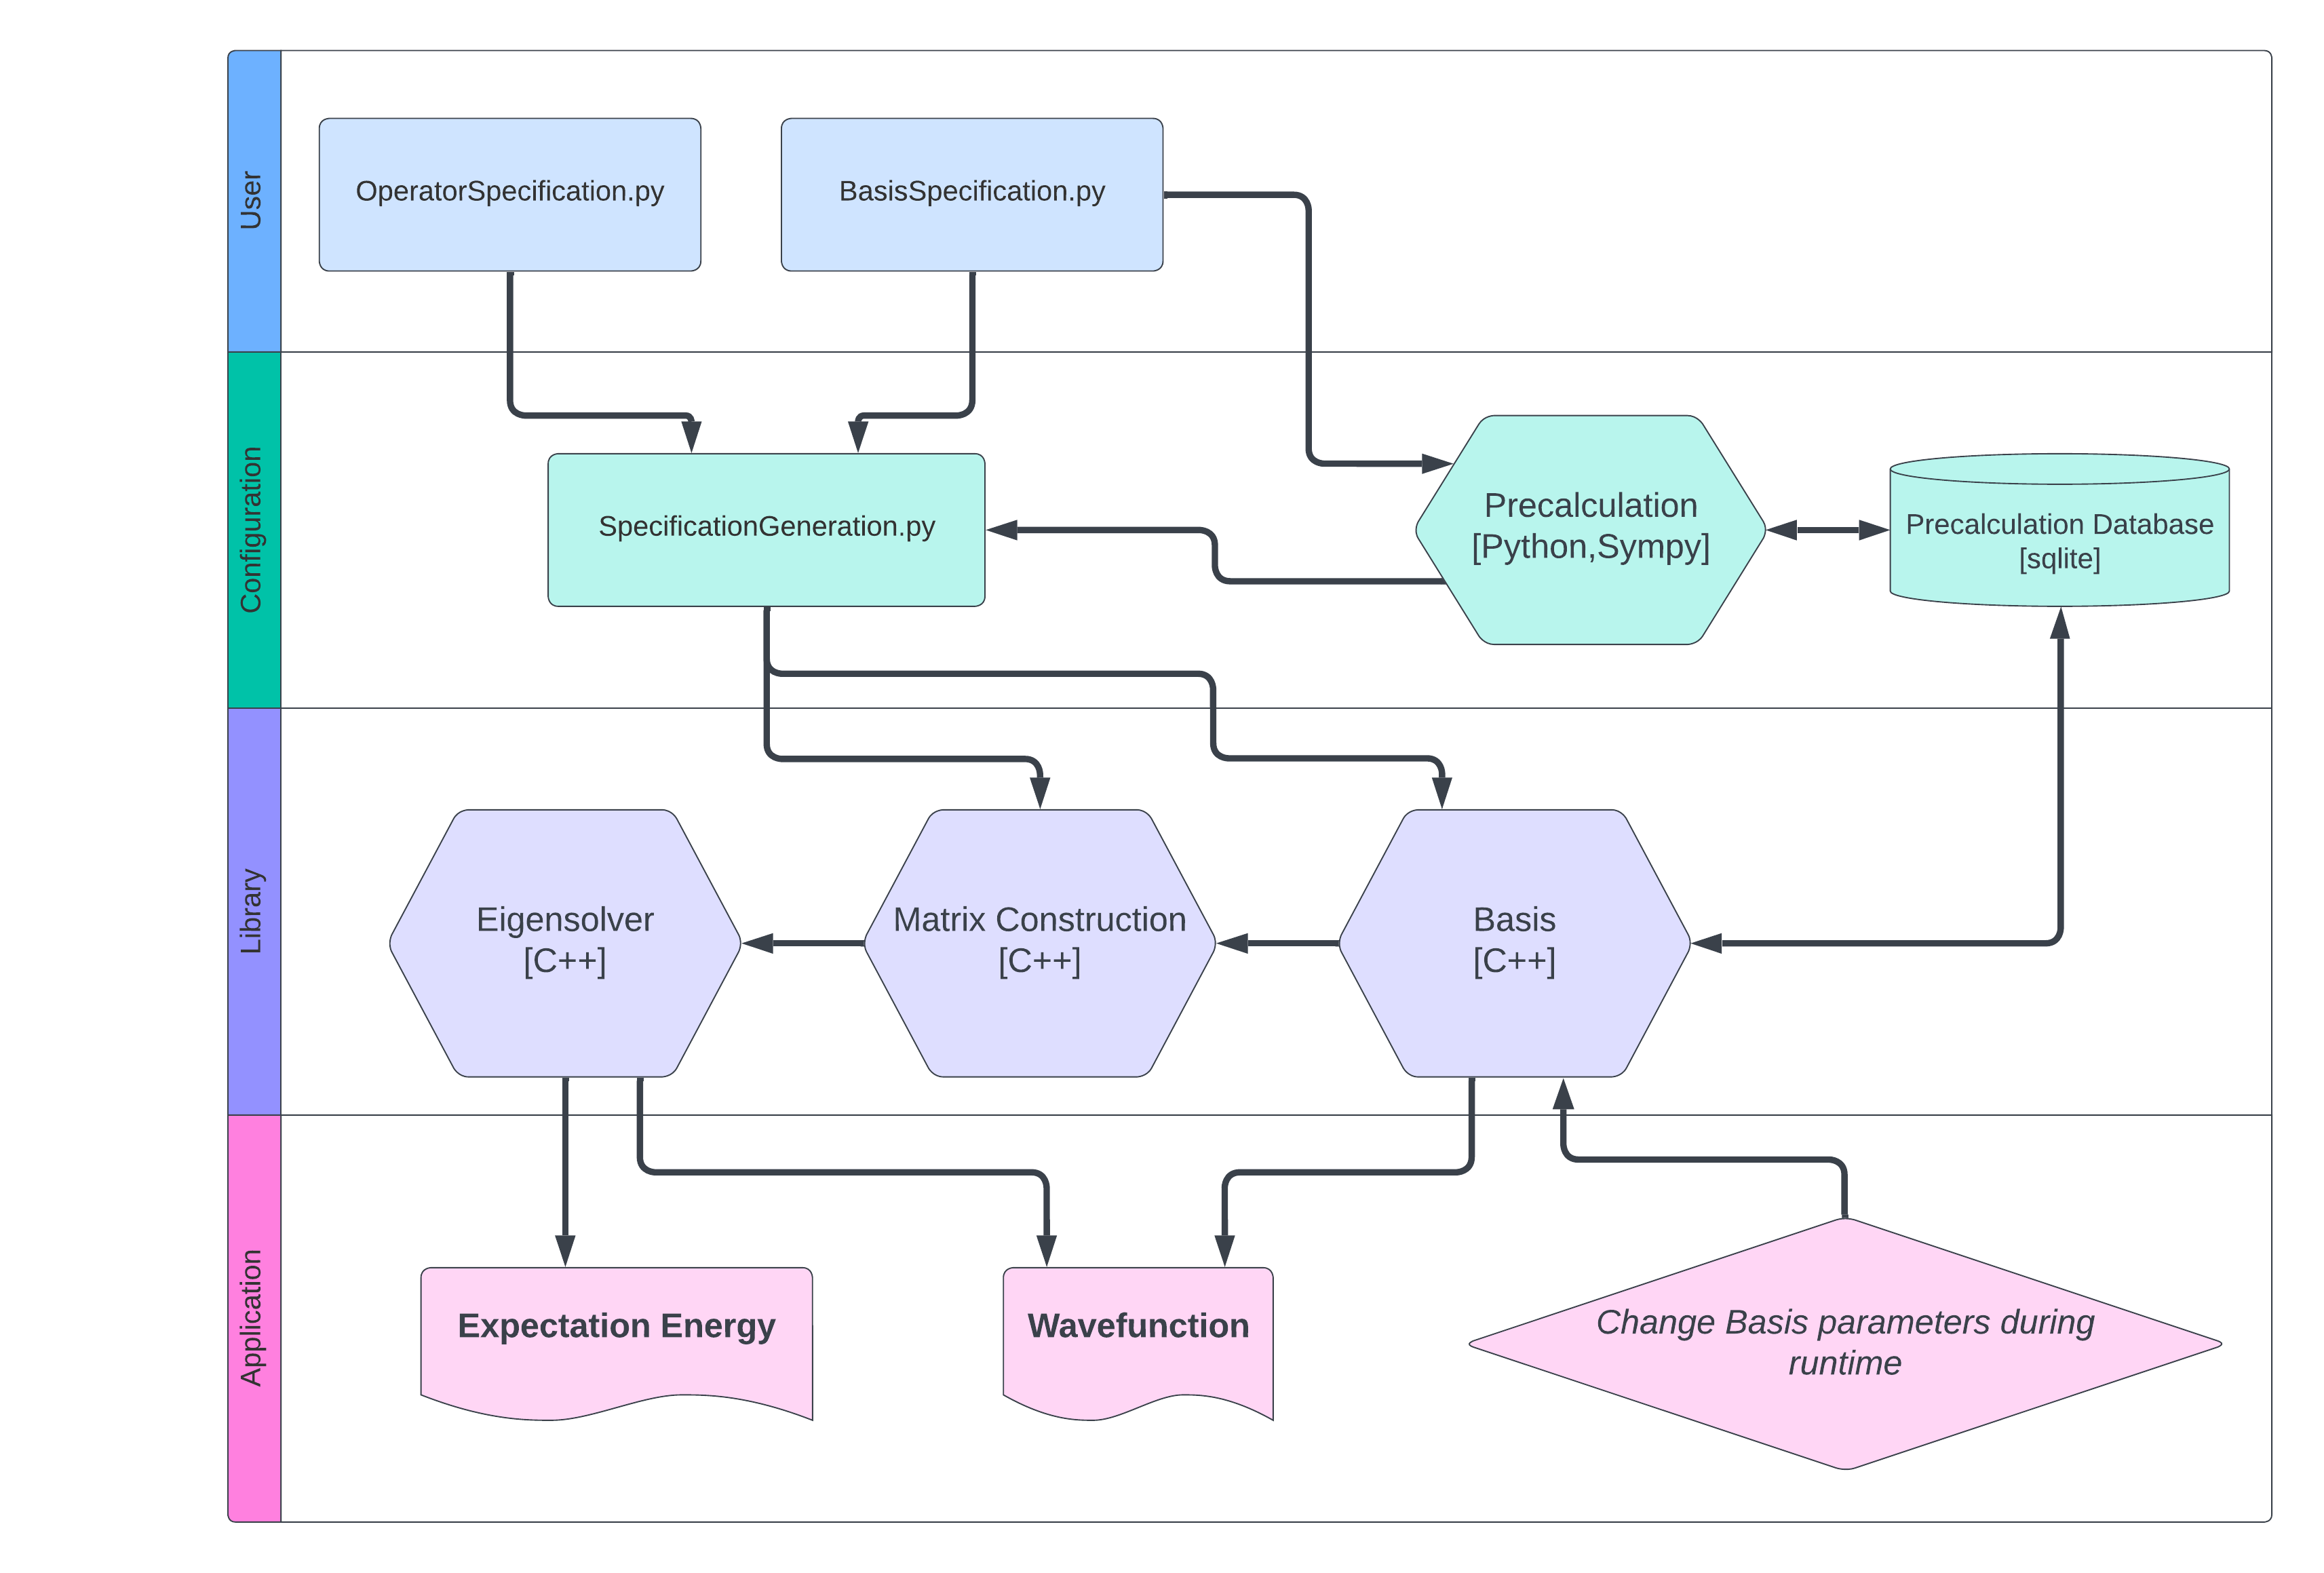
\includegraphics[width=150mm]{
        CantankerousImpuritySoftwareStructure_ver2.png
    }
    \caption{Overall Cantankerous Impurity structure.}
\label{flowchart}
\end{figure}

In figure \ref{flowchart} we present a map of the flow and structure of
Cantankerous Impurity.
    \section{Precalculation}
    \label{section:precalculation}
        % % \documentclass[aps, prl, preprint]{revtex4-2}
% \documentclass{report}

% \usepackage{graphicx}
% \usepackage{dcolumn}
% \usepackage{array,multirow,adjustbox}
% \usepackage{bm}
% \usepackage{amsfonts, amssymb, amsmath}
% \usepackage{braket}
% \usepackage{siunitx}

% % \newcommand{\ket}[1]{\textstyle \left| #1 \right\rangle \displaystyle}
% % \newcommand{\bra}[1]{\textstyle \left\langle #1 \right| \displaystyle}
% % \newcommand{\braket}[2]{\textstyle \left\langle #1 \left|  #2 \right\rangle\right. \displaystyle}

% \let\originalleft\left
% \let\originalright\right
% \renewcommand{\left}{\mathopen{}\mathclose\bgroup\originalleft}
% \renewcommand{\right}{\aftergroup\egroup\originalright}

% \newcommand{\im}{\mathrm{i}}
% \newcommand{\e}{\mathrm{e}}
% \newcommand{\pwrt}[2]{\frac{\partial #1}{\partial #2}}
% \newcommand{\diff}{\mathrm{d}}

% \DeclareMathOperator{\atantwo}{atan2}

% \begin{document}

The most unique feature of Cantankerous Impurity, as far as it is known to the
author, is the use of the exact Laguerre polynomials in our basis functions without truncations. As such, we wish to devote some time to discussion of the computations use of these polynomials entails.

For our purposes, we have defined the \emph{precalculated coefficients} in
Appendix \ref{appendix:elements} as a set of numbers that must be computed
analytically to get accurate results, and are important parts of the integrands
used to compute the matrix elements. These computations of analytical numbers
are potentially time consume; as such, we have chosen to assemble these
coefficients as needed when the program is compiled. The precalculated
coefficients are then stored in a database and called into active memory at the
start of the program run. Only those coefficients needed to represent the
user-designated \emph{sub-} and \emph{superbasis} states are loaded into active
memory. As this database persists from run to run, recompiling the program to
change various physical or technical parameters does not necessitate adding to
the database. This is only required if states with new discrete indices are
added to the basis being considered.

We note many of these values we are computing must be stored as exact analytical
values. For this reason, we have implemented much of this code within SymPy,
storing our values as SymPy objects which represent exact quantities and may be
manipulated according to the rules of conventional computer algebra implemented
within SymPy. We will also find that the collection of values we are computing
and storing have coefficients that don't make conventional rectangular storage
easy. As such, much of these arrays of values are implemented as Python
dictionaries, allowing easy association between a particular set of coefficients
and the desired analytical SymPy object.

As derived in Appendix \ref{appendix:elements}, these coefficients go as
\begin{align}
\mathfrak{A}_{\mathfrak{d}\left(su\right)_{01}w}
    &=
        \left(-1\right)^{u_{0}+u_{1}+w}
        \Gamma\left[
            \frac{\mathfrak{h}_{\mathfrak{d}\left(s\right)_{01}}}{W}+w
        \right]
        \mathfrak{A}_{\left(su\right)_{01}w}^{\prime}
\tag{\ref{appendix:elements:precalc-coeffs-0}}
,\\
\mathfrak{A}_{\left(su\right)_{01}w}^{\prime}
    &=
        \sum
        _{ v = \text{Max}\left[0,\mathfrak{K}_{0}+u_{1}-w\right] }
        ^{ \text{Min}\left[
            \mathfrak{K}_{0}-u_{0},\mathfrak{K}_{0}+\mathfrak{K}_{1}-w
        \right] }
        \mathfrak{A}_{\left(su\right)_{0}v}^{\prime\prime}
        \mathfrak{A}
        _{\left(su\right)_{1}\left(\mathfrak{K}_{0}+\mathfrak{K}_{1}-v-w\right)}
        ^{\prime\prime}
\tag{\ref{appendix:elements:precalc-coeffs-1}$^{\prime}$}
,\\
\mathfrak{A}_{suv}^{\prime\prime}
    &=
        \frac{1}{\sqrt{k!\left(k+\mathfrak{l}\right)!}}
        \begin{pmatrix}\mathfrak{K}\\u\end{pmatrix}
        \begin{pmatrix}\mathfrak{K}-u\\v\end{pmatrix}
        \left(k+\mathfrak{l}\right)^{\underline{v}}
        \left(1 + \mathfrak{u}\mathfrak{I}_{sv}\right)
.
\tag{\ref{appendix:elements:precalc-coeffs-2}$^{\prime}$}
\end{align}
The primed equations above and below feature minor modifications to their forms
as compared to the versions attested in Appendix \ref{appendix:elements} but as
the changes are straightforward, we do not anticipate this will generate
confusion. We show in Appendix \ref{appendix:elements} that
\begin{align}
\mathfrak{I}_{sv}
    &=
        \frac
        { \mathfrak{H}_{sv}^{\prime} }
        {\left(k+\mathfrak{l}+2-v\right)\left(k+\mathfrak{l}+1-v\right)}
            -
        1
\tag{\ref{appendix:elements:precalc-coeffs-3}}
,\\
\mathfrak{H}_{sv}^{\prime}
    &=
        \sum_{t=0}^{\text{Min}\left[v,3+\delta_{s\bar{1}}\right]}
        v^{t}
        \mathfrak{G}_{st}
\tag{\ref{appendix:elements:precalc-coeffs-4}}
,\\
\mathfrak{G}_{st}
    &=  
        g_{kl,s\left(1+\delta_{s\bar{1}}-t\right)}
        \sqrt
        {
            \frac{ \left(k+1+\delta_{s\bar{1}}-t\right)! }{ k! }
            \frac
            { \left(k+\mathfrak{l}+2-t\right)! }
            { \left(k+\mathfrak{l}\right)! }
        }
\tag{\ref{appendix:elements:precalc-coeffs-5}}
.
\end{align}
As mentioned in Appendix \ref{appendix:elements}, the formulae to find the
values of $g_{kl,st}$ are cumbersome to write and derive. The formulae for these
coefficients may be found in the
\href{https://gitlab.com/cantankerous-impurity/Documentation/-/tree/core/SUNY--Buffalo/Dissertation/Supplementary%20Materials?ref_type=heads}{Supplementary Materials}.

When the appropriate values of the coefficients $g$ are used we may write
\begin{align}
\mathfrak{I}_{\bar{1}v}
    & =
        -(k+1+v)(k+2+v)+2v-1
        +
        \delta_{W,1}\mathfrak{I}_{\bar{1}v}^{\prime}
,\\
\mathfrak{I}_{\bar{1}v}^{\prime}
    & =
        \frac{6v(k+2-v)}{\alpha+1-v}
            +
        \frac{12v(v-1)}{\alpha+2-v}
,\\
\mathfrak{I}_{0v}
    & =
        k+v
            +
        \frac
        {2v\left(k-\delta_{W,1}\left(v-1\right)+\delta_{W,2}v\right)}
        {\alpha+1-v}
            +
        \delta_{W,1}\frac{4(v-1)v}{\alpha+2-v}
,\\
\mathfrak{I}_{1v}
    & =
        k-x
            +
        \frac{2x(2x(k+\delta_{W,2}-x)+\delta_{W,1})}{\alpha+1-x}
            +
        \frac{4x(-k+x-\delta_{W,2})(x-1)}{\alpha+2-x}
.
\end{align}
So let's consider what information is required to know from each state to know
which precalculated coefficients to precalculate. To calculate
$\mathfrak{I}_{sv}$ we need to specify a given set of $ \left(W;kl\right) $. Once
we know those three pieces of information, we know that the coefficients to
calculate for $\mathfrak{I}_{sv}$ have $ 0 \le v \le k + 1 + \delta_{s\bar{1}}$
and $ s \in \left\{-1,0,+1\right\}$.

We introduce the following notational convention. In this section, \emph{bolded}
quantities represent sequences or arrays of objects. These objects themselves
depend upon certain quantities we can use to denote to identify a particular
entry of the array, which we will consider to be \emph{array indices}. Any
remaining quantities necessary to compute the values of a given array will be
called \emph{array parameters}. As array indices are conventionally denoted as
subscripts, we will denote parameters as superscripts. Of course, the
distinction between these two concepts is somewhat arbitrary, and depends upon
the requirements to implement the structures in code. In the following
discussion, any particular choice to identify as a value as a array index or
array parameter should be considered provisional, and ultimately dependent upon
the code's final production implementation. Finally, it is possible to imagine
multidimensional arrays constructed as an array or arrays, or as a
concatenation of arrays. In that case, we can imagine an array parameter in the
subarray becoming an array index in the larger superarray.

When we define each bold symbol, we will use set notation to identify and give
the limits of the array indices. For $\bm{\mathfrak{I}}$ we give
\begin{equation}
\bm{\mathfrak{I}}^{\left(W;kl\right)}
    \coloneqq
        \left\{
            \mathfrak{I}_{sv}
                |
            s = -1,0,1 \text{ and }
            0 \le v \le k + 1 + \delta_{s\bar{1}}
        \right\}
\end{equation}

So for the basis specified by the user, the precalculation coefficient checker
must determine if $ \bm{\mathfrak{I}}^{\left(W;kl\right)} $ has been calculated
for all $ \left( W; lk \right) $ present in the specification of the user's
basis. We expect that, while it is possible that a user may wish to have a
subbasis or superbasis that employs a mix of $W = 1$ and $W = 2$, we expect the
likelihood of such an event to be low. Right now our program doesn't implement
mixing states of different $W$, and we require the user to specify if their
overall superbasis uses $W = 1$ (Slater) or $W = 2$ (Gaussian) envelope
functions exclusively. A positive integer $W \ne 1,2$ is possible, but well
beyond the scope of the current software.

As we move up the computation chain, our next goal will be to calculate
$\mathfrak{A}^{\prime\prime}$. This coefficient, like before, depends on the
$\left(W;kl\right)$ quantities from only one state. However, this coefficient
will have two forms depending on whether the kinetic toggle $\mathfrak{u} =
0$ or $\mathfrak{u}=1$. 

To simplify this, we may consider the following
\begin{equation}
\mathfrak{A}_{suv}^{\prime\prime\left(\mathfrak{j}\right)}
    \coloneqq
        \left(
            \frac{1}{\sqrt{k!}}
            \begin{pmatrix}k + \mathfrak{j}\\u\end{pmatrix}
            \begin{pmatrix}k + \mathfrak{j} - u\\v\end{pmatrix}
        \right)
        \frac
        {\left(k+\mathfrak{l}\right)^{\underline{v}}}
        {\sqrt{\left(k+\mathfrak{l}\right)!}}
.
\end{equation}
Above, we grouped factors of the formula to point out places where defining and
memoizing relevant subfunctions used to compute the coefficients would be very
useful. For example we can consider the function
\begin{equation}
\mathcal{V}_{x,v}
    \coloneqq
        \frac{\left(x\right)^{\underline{v}}}{\sqrt{x!}}.
\end{equation}
We note that we can use $\mathcal{V}_{k+\mathfrak{l},v}$ when computing part of
the above equation. We can expect integer $x=k+2l+2$ when $W = 1$ and
half-integer $x=k+l+\frac{1}{2}$ when $W = 2$. It is clear that multiple
particular combinations of $\left(W;kl\right)$ could correspond to the same
value of $k + \mathfrak{l}$. Memoizing a function is a computer science term
that describes implementing a function with the ability to record and recall
some aspect of past computations, such as return values or earlier internal
states. This can be quite convenient when optimizing or trying to speed up a
computation, such as those of the precalculated coefficients. In this document
we are most interested in the broader program structure and flow. While we will
not often describe the fine details of specific computations, such as a specific
definition and memoizing scheme for useful subfunctions, we note that some
notational and stylistic choices in the following sections are made to make
clear opportunities to optimize computation with memoization. 

Above, $\mathfrak{A}^{\prime\prime\left(\mathfrak{j}\right)}$ will have
$\mathfrak{j} = 0, 1, 2$. The value of $\mathfrak{j}$ determines the limits of
$s$, $u$, and $v$. When $\mathfrak{j} = 0$ it must be that $\mathfrak{u} = 0$ so
$\mathfrak{K} = k$ and $s = 0$. Taking into account the possible values of
$\mathcal{A}^{\prime\prime}$ given a particular value of $\mathfrak{j}$, we can
compute the following arrays of values. 

An important accessory set to define is the set of values $\left(u,v\right)$ to
run over as indices. We also wish to define a set that includes the possible
tuples $\left(s,u\right)$ for a given $\mathfrak{u} = 0, 1$. Let us define
\begin{align}
\bm{\mathfrak{S}}^{\left(\mathfrak{u}\right)}
    &\coloneqq
        \left\{
            s \in \mathbb{Z}
                |
            -\mathfrak{u} \le s \le +\mathfrak{u}
        \right\}
,\\
\bm{\mathfrak{U}}^{\left(\mathfrak{K}\right)}
    &\coloneqq
        \left\{ u \in \mathbb{Z} | 0 \le u \le \mathfrak{K} \right\}
,\\
\bm{\mathfrak{V}}^{\left(\mathfrak{K}\right)}
    &\coloneqq
        \left\{
            \left(u,v\right)
                |
            u \in \bm{\mathfrak{U}}^{\left(\mathfrak{K}\right)}
                    \text{ and }
            v \in \bm{\mathfrak{U}}^{\left(\mathfrak{K}-u\right)}
        \right\}
.
\end{align}
This provides a convenient short-hand we can refer to at points later in this
documentation. Note that $\bm{\mathfrak{V}}^{\left(\mathfrak{K}\right)}$ is not
a conventional rectangular array, as the limits of the trailing dimension $v$
depends on the value of the leading dimension $u$. This will be true of many of
the arrays generated for this section.

Our array of the $\bm{\mathfrak{A}} _{ W;kl } ^{ \prime\prime } $ values with
indices $s, u, v$, and $\mathfrak{u}$ may be define as
\begin{equation}
\bm{\mathfrak{A}}_{W;kl}^{\prime\prime}
    \coloneqq
        \left\{
            \mathfrak{A}
            _{suv}
            ^{\prime\prime\left(\mathfrak{u}+\delta_{s\bar{1}}\right)}
                |
            \left(u,v\right)
                \in
            \bm{\mathfrak{V}}^{\left(k+\mathfrak{u}+\delta_{s\bar{1}}\right)}
                \text{ and }
            \mathfrak{u} \in \left\{ 0,1 \right\}
                \text{ and }
            s \in \mathfrak{S}^{\left(\mathfrak{u}\right)}
        \right\}
.
\end{equation}
Since we expect every use of the code to include operators with both $
\mathfrak{u} = 0 $ and $ \mathfrak{u} = 1 $ both will be needed during each
program run. As such, we treat it as an array index rather then an array
parameter depending upon the user's operator specification.

Up to now, we've been dealing with precalculated coefficients that depend only
upon parameters from a single state in the basis. As we move forward to the
coefficients that depend upon pairs of states, we can exploit some of the
symmetry property of the coefficients. We note it may be shown that
\begin{equation}
\mathfrak{A}
_{\left(su\mathfrak{u}\right)_{0}\left(su\mathfrak{u}\right)_{1}w}
^{\left(W;\left(lk\right)_{0}\left(lk\right)_{1}\right)}
    =
        \mathfrak{A}
        _{\left(su\mathfrak{u}\right)_{1}\left(su\mathfrak{u}\right)_{0}w}
        ^{\left(W;\left(lk\right)_{1}\left(lk\right)_{0}\right)}
\end{equation}
This symmetric behavior allows us to roughly half the number of precalculated
coefficients with an efficient implementation. Since two different sets of
indices map to the same final value, it's necessary to have a consistent rule to
be able map either of the two possibilities to the same final value without
repeating the storage of that value unnecessarily. This is equivalent to
assigning an ordering scheme to each possible set of $\left(kl\right)$
indices.In general, we do not presume a "canonical" ordering to the possible
values of $\left(kl\right)$ a user may use to construct a basis. Instead, the
database itself keeps an list specifying the order of $\left(kl\right)$ as they
are added. We expect that changes to the order of states within the basis made
by the user within the configuration phase of deployment to be invisibly handled
by the Precalculation module. More details may be found in the forthcoming
Supplementary Materials.

In this document, we won't pay too much attention to the state order. It is
sufficient to realize that, for given pair of states, our code implementation
will ensure that the appropriate values are calculated and dispatched
appropriately as efficiently as necessary. In any case, now that we are
considering the two-state precalculated coefficients, it's worthwhile to define
accessory sets of indices that go as
\begin{align}
\bm{\mathfrak{W}}^{\left(\mathfrak{u}\right)}
    &=
        \left\{
            \left(s,u\right)
                |
            s \in \mathfrak{S}^{\left(\mathfrak{u}\right)}
                \text{ and }
            u
                \in 
            \mathfrak{U}^{\left(k+\mathfrak{u}+\delta_{s_{0\bar1}}\right)}
        \right\}
,\\
\bm{\mathfrak{Y}}^{\left(\mathfrak{u}\right)}
    &=
        \left\{
            \left(\left(s,u\right)_{01}, w^{\prime}+u_{0}+u_{1}\right)
                |
            \left(s,u\right)_{01}
                \in
            \bm{\mathfrak{W}}^{\left(\mathfrak{u}\right)_{01}}
                \text{ and }
            w^{\prime}
                \in
            \bm{\mathfrak{U}}
            _{
                \mathfrak{K}_{0}
                    +
                \mathfrak{K}_{1}
            }
        \right\}
.
\end{align}
where we recall that, for a given basis state, $\mathfrak{K} = k + \mathfrak{u}
+ \delta_{s\bar{1}}$.

The final step necessary to calculate the general precalculated coefficients is
\begin{equation}
\mathfrak{A}
_{\left(su\right)_{01}w}
^{\left(W\mathfrak{d};\left(lks\right)_{0}\left(lks\right)_{1}\right)}
    =
        \left(-1\right)^{u_{0}+u_{1}+w}
        \Gamma\left[
            \frac{\mathfrak{h}_{\mathfrak{d}\left(s\right)_{01}}}{W}+w
        \right]
        \mathfrak{A}_{\left(su\right)_{01}w}^{\prime}
\tag{\ref{appendix:elements:precalc-coeffs-0} }
\end{equation}
We note that $\mathfrak{h}_{\mathfrak{d}\left(s\right)_{01}} = l_{0} + l_{1}
-\delta_{W1}\left(\mathfrak{u}_{0}+\mathfrak{u}_{1}\right) + \mathfrak{d} + 3$.
This is straightforward to calculate from $
\mathfrak{A}_{\left(su\right)_{01}w}^{\prime} $ with one caveat. Up till now,
the precalculated coefficients haven't depended upon the potential model.
However, with the introduction of $\mathfrak{d}$ into the formulae, we will need
knowledge of the user-made operator specification. Thus, both the basis and the
potential model need to be specified at compile time. We make no assumptions
about $\mathfrak{d}$ other than $\mathfrak{d}\in\mathbb{R}$ and $\mathfrak{d} >
-2$ as $\mathfrak{d} \le 2$ makes the matrix element integrals divergent.

Finally, the summations found in the integrand of our matrix elements will
simplify when certain conditions are met, something we expect will emerge in
most use cases of the software. One of the difficulties in using the terms of
the Laguerre polynomials emerges in these cases, as we end up needing to compute
the summation of sequences of alternating sign. Even using the Kahan summation
algorithm, we find these summations are very ill-conditioned when computed using
floating point numbers. As such, rather then computing these summations in the
matrix element integrand, we compute coefficients that may be used in  the
simplified sums. To wit, for each $\mathfrak{A}$ we must also compute the
following values.

\begin{align}
\mathfrak{A}_{\left(s\right)_{01}uw}
    &=
        \left[ \sum_{u=0}^{\mathfrak{K}} \right]_{01}
        \delta_{u,u_{0}+u_{1}}
        \left(-1\right)^{u_{0}}
        \mathfrak{A}_{\left(su\right)_{01}w}
,\\
\mathfrak{A}_{\left(s\right)_{01}uw}^{\prime}
    &=
        \left[ \sum_{u=0}^{\mathfrak{K}} \right]_{01}
        \delta_{u,u_{0}+u_{1}}
        \mathfrak{A}_{\left(su\right)_{01}w}
,\\
\mathfrak{A}_{\left(s\right)_{01}w}
    &=
        \mathfrak{A}_{\left(s0\right)_{01}w}
,\\
\mathfrak{a}_{\left(s\right)_{01}u}
    &=
        \left[ \sum_{u=0}^{\mathfrak{K}} \right]_{01}
        \sum_{w=u}^{\mathfrak{K}_{0}+\mathfrak{K}_{1}}
        \delta_{u,u_{0}+u_{1}}
        \left(-1\right)^{u_{0}}
        \mathfrak{A}_{\left(su\right)_{01}w}
,\\
\mathfrak{a}_{\left(s\right)_{01}u}^{\prime}
    &=
        \left[ \sum_{u=0}^{\mathfrak{K}} \right]_{01}
        \sum_{w=u}^{\mathfrak{K}_{0}+\mathfrak{K}_{1}}
        \delta_{u,u_{0}+u_{1}}
        \mathfrak{A}_{\left(su\right)_{01}w}
,\\
\mathfrak{a}_{\left(s\right)_{01}}
    &=
        \sum_{w=u}^{\mathfrak{K}_{0}+\mathfrak{K}_{1}}
        \mathfrak{A}_{\left(s0\right)_{01}w}
.
\end{align}
    

\chapter{Benchmarking}
\label{chapter:results}
    \section{Statically screened Coulomb potential}
        % % % \documentclass[aps, prl, preprint]{revtex4-2}
% % \documentclass{report}

% % \usepackage{graphicx}
% % \usepackage{dcolumn}
% % \usepackage{array,multirow,adjustbox}
% % \usepackage{bm}
% % \usepackage{amsfonts, amssymb, amsmath}
% % \usepackage{braket}
% % \usepackage{siunitx}

% % % \newcommand{\ket}[1]{\textstyle \left| #1 \right\rangle \displaystyle}
% % % \newcommand{\bra}[1]{\textstyle \left\langle #1 \right| \displaystyle}
% % % \newcommand{\braket}[2]{\textstyle \left\langle #1 \left|  #2 \right\rangle\right. \displaystyle}

% % \let\originalleft\left
% % \let\originalright\right
% % \renewcommand{\left}{\mathopen{}\mathclose\bgroup\originalleft}
% % \renewcommand{\right}{\aftergroup\egroup\originalright}

% % \newcommand{\im}{\mathrm{i}}
% % \newcommand{\e}{\mathrm{e}}
% % \newcommand{\pwrt}[2]{\frac{\partial #1}{\partial #2}}
% % \newcommand{\diff}{\mathrm{d}}

% % \DeclareMathOperator{\atantwo}{atan2}

% % \title{An open source software package to compare and extend effective mass models of the phosphorous donor in silicon}
% % \author{Luke Pendo}
% % \date{}

% % \begin{document}

\subsection{Exploring Single Eigenstates, Single-Valley}

The first feature of our program we want to explore is a benchmarking against
the single-valley Kohn-Luttinger and Faulkner results. Below we present plots of
a single subbasis as we sweep the radial and anisotropic variational parameters
of that subbasis. In the single state basis, our program generates results
identical to what Kohn-Luttinger found for their ground states. However, as we
increase the size of the basis the energy surface flattens. This is to be
expected as the basis coefficients themselves are variational parameters that
are set by the process of computing the solution to the generalized eigenvalue
problem. In short, as the basis size increases, the number of variational
parameters set by the eigensolver increases, while the number of free parameters
per subbasis stays the same. This means the importance of the free variational
parameters decreases.

\begin{figure}
\centering
\subfloat[Basis: (0,0,0)]
{
    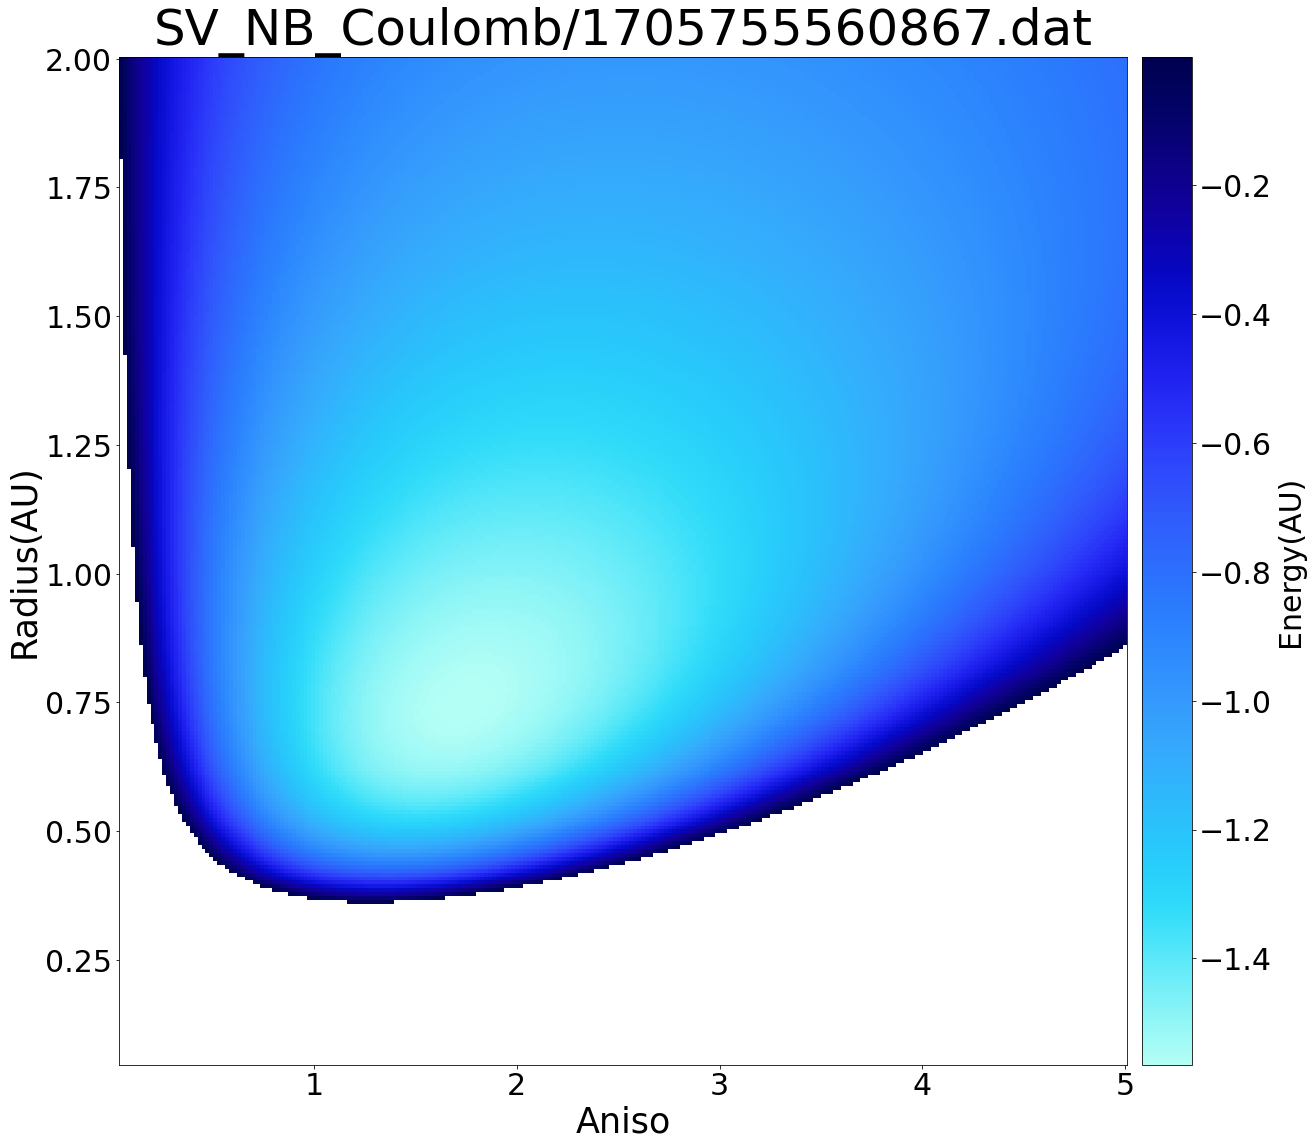
\includegraphics[width=64mm]{1705755560867.png}
}
\subfloat[Basis: (0,0,0),(0,0,1),(0,0,2)]
{
    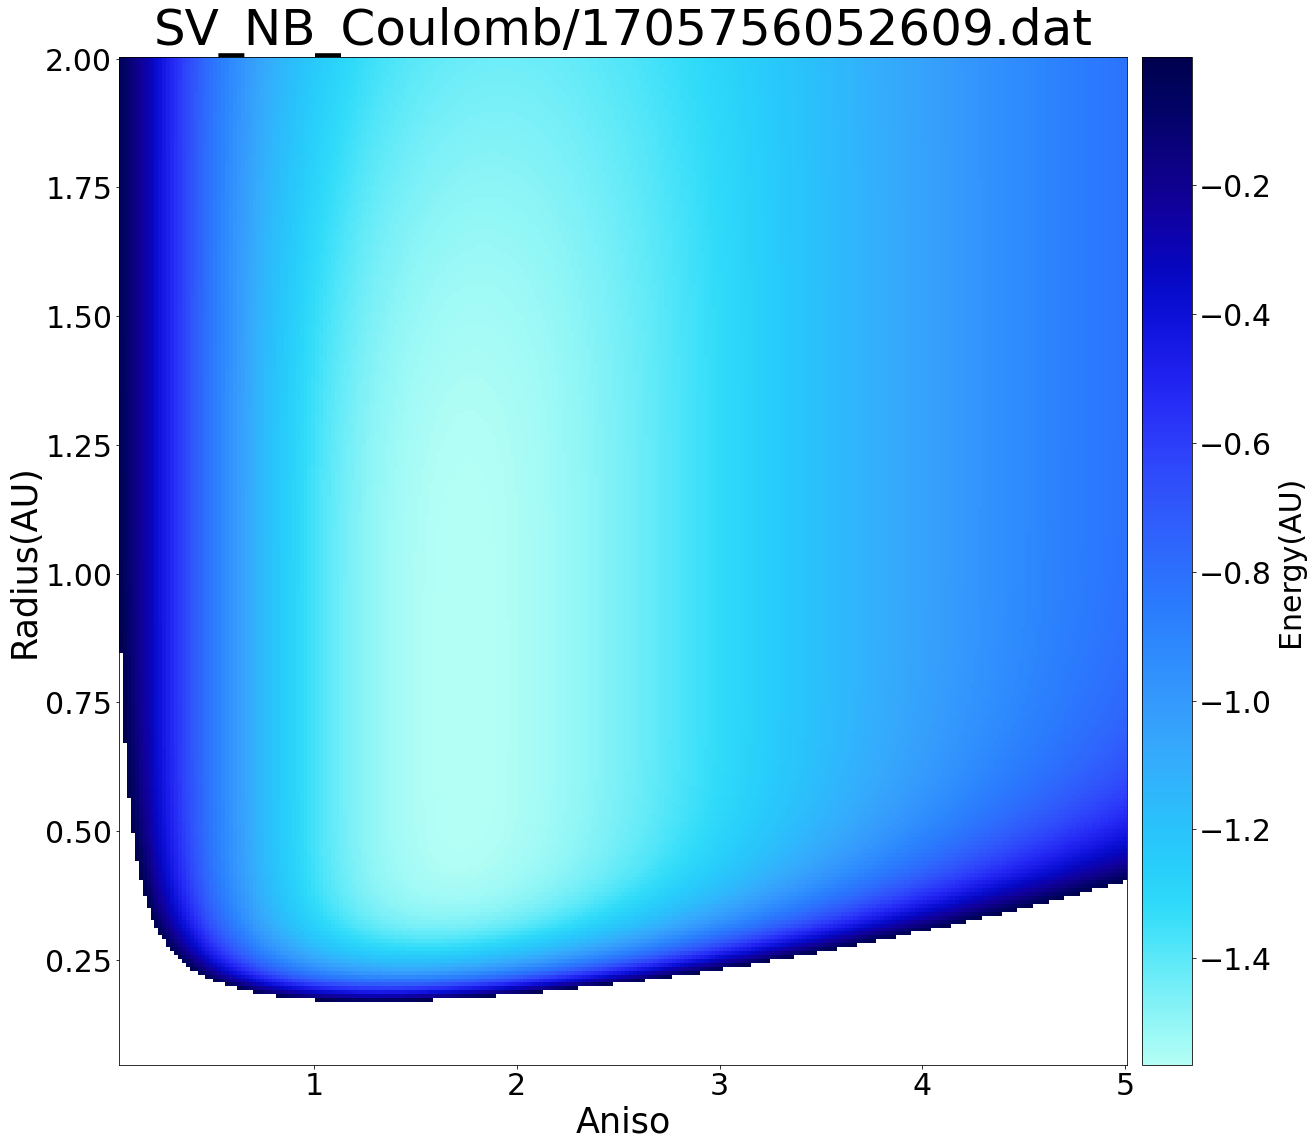
\includegraphics[width=64mm]{1705756052609.png}
}
\hspace{0mm}
\subfloat[Basis: (0,0,0),(0,2,0),(0,4,0)]
{
    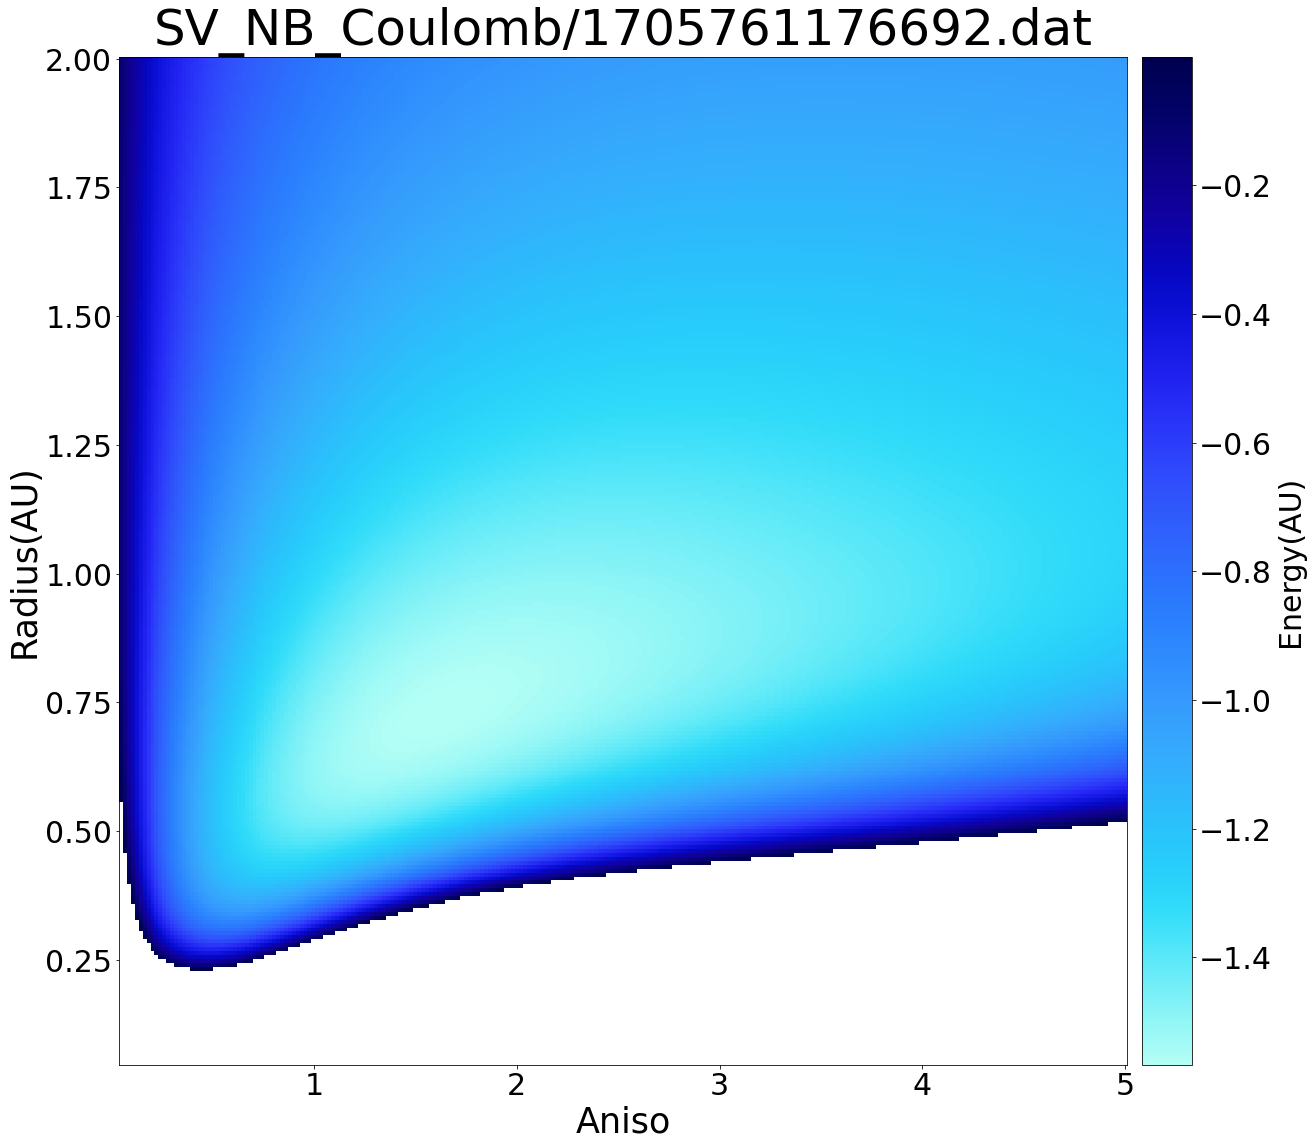
\includegraphics[width=64mm]{1705761176692.png}
}
\subfloat[Basis: (0,0,0),(0,0,1),(0,0,2),(0,2,0),(0,2,0),(0,4,0)]
{
    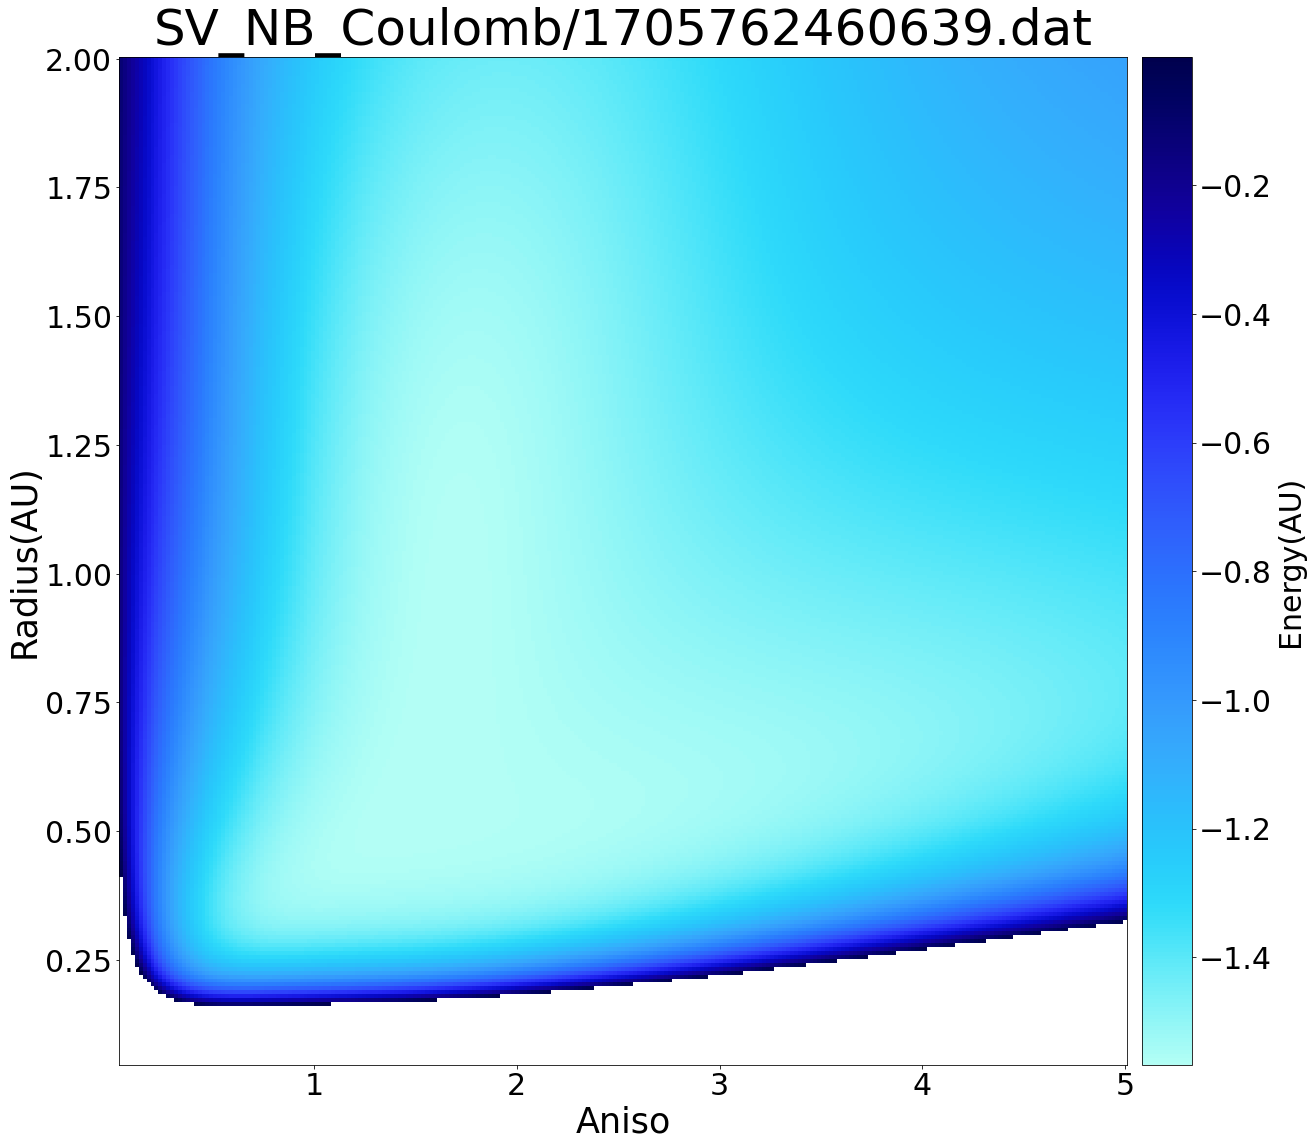
\includegraphics[width=64mm]{1705762460639.png}
}
\hspace{0mm}
\subfloat[Basis: (12 states) \newline $0\le k\le 2,l=\{0,2,4,6\},m=\{0\}$]
{
    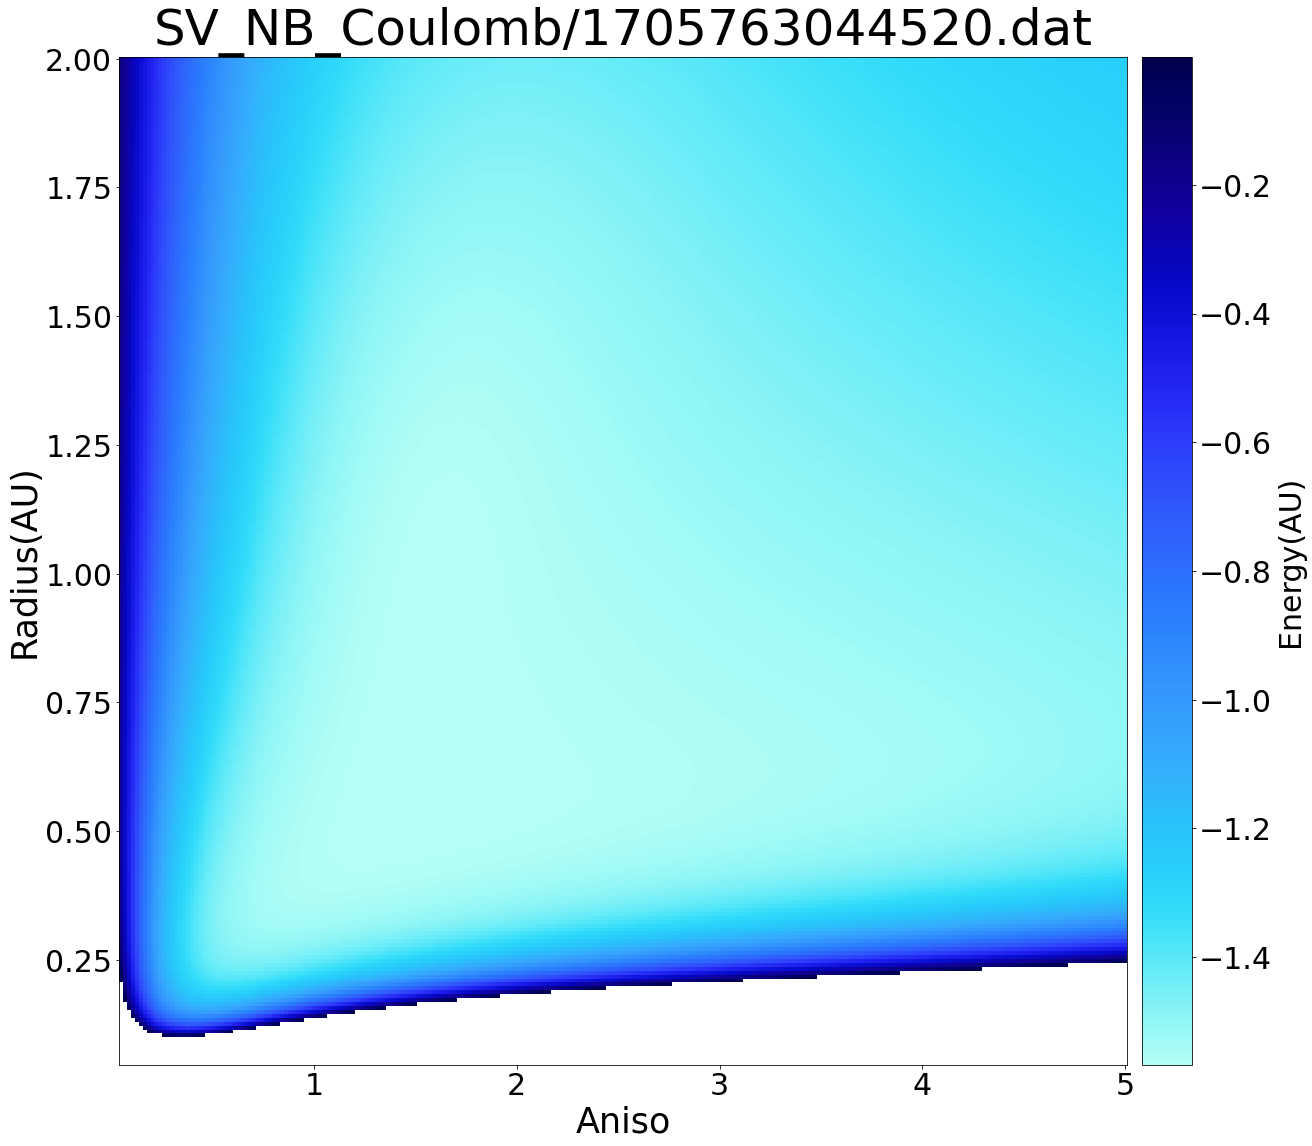
\includegraphics[width=64mm]{1705763044520.png}
}
\subfloat[Basis: (16 states) \newline $0\le k \le 3,l=\{0,2,4,6\},m=\{0\}$]
{
    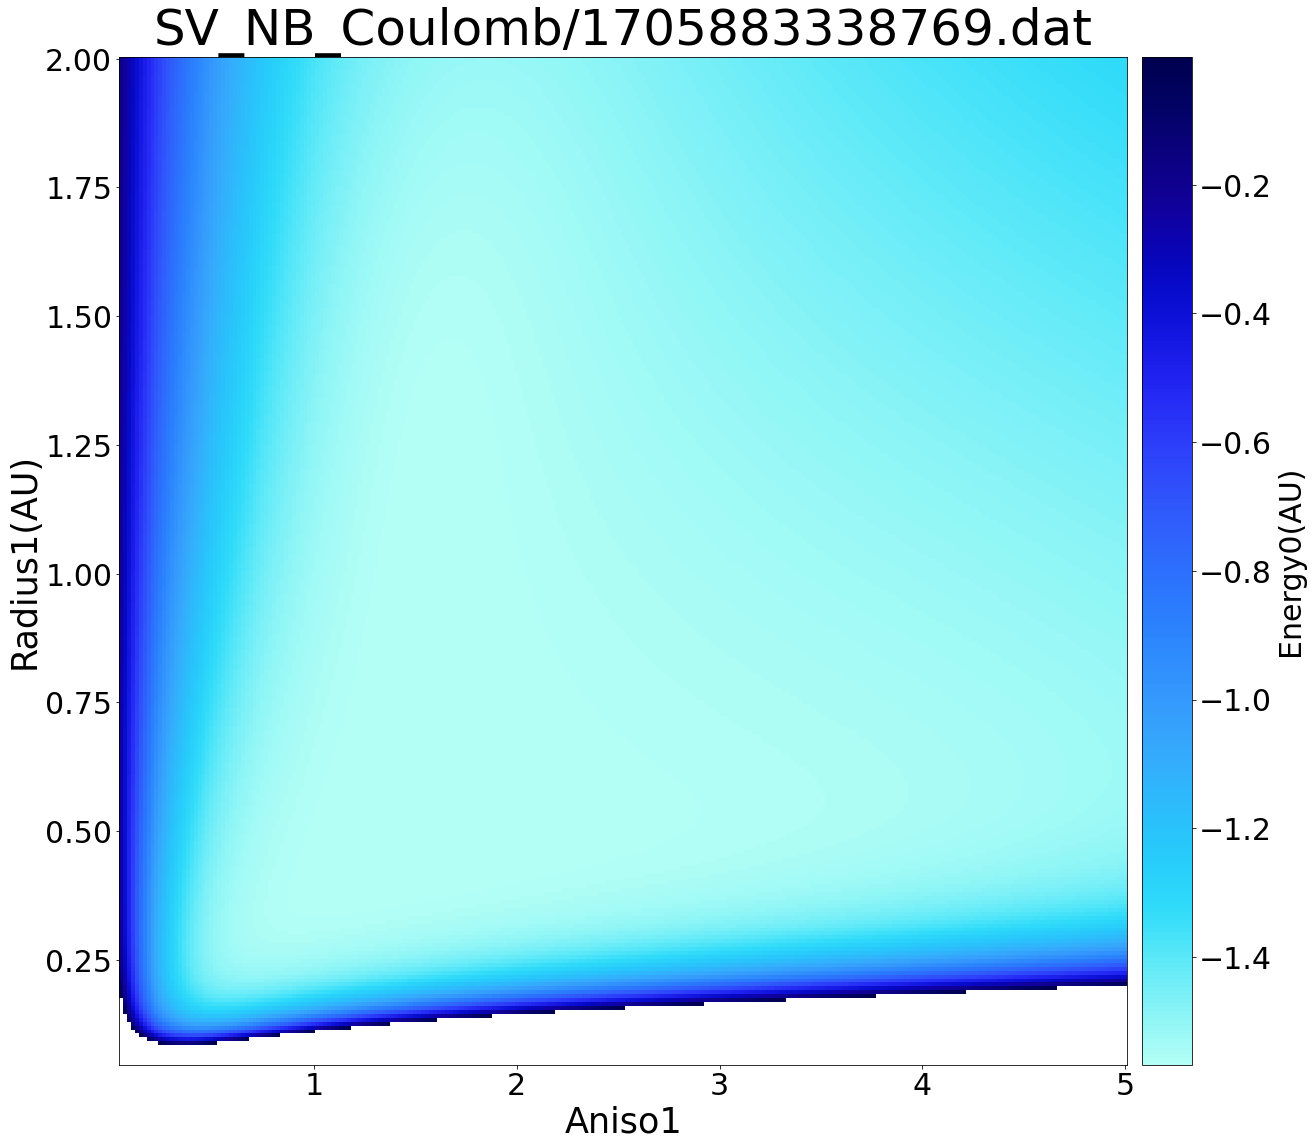
\includegraphics[width=64mm]{1705883338769.png}
}
\caption{This figure shows the effect of basis size on the related variational problem. As the basis size increases, the energy surface becomes less sensitive to changes in the radial and anisotropic parameters within a certain neighborhood of the parameter space.}
\label{sv-basis-size}
\end{figure}

Benchmarking of this software is on-going, especially as regards to the
multi-valley states. In particular, there are still ambiguities in regards to
the use of the Bloch functions within Cantankerous Impurity. Further
benchmarking results can be found in the \href{https://gitlab.com/cantankerous-impurity/Documentation/-/tree/core/SUNY--Buffalo/Dissertation/Supplementary%20Materials?ref_type=heads}{Supplementary Materials}.



\chapter{Potential for future work}

\appendix
\chapter*{Appendix}
\addcontentsline{toc}{chapter}{Appendices}
\renewcommand{\thesection}{\Alph{section}}
\renewcommand{\theequation}{\Alph{section}.\arabic{equation}}
    \section{System units}
    \label{appendix:units}
        % \subsection{Atomic units}
For explicit numerical work, it is convenient to use a unitless formulation. In
much the same way as is done in the standarnd treatment of the hydrogen atom
problem, we introduce the unitful constants $\mathfrak{E}$ for energy and $\mathfrak{r}$ for
length. We define these constants such that
\begin{equation}
  \mathfrak{E}
  \equiv
  \frac{\hbar^2}{2 m_\perp \mathfrak{r}^2}
  =
  \frac{e^2}{8\pi \epsilon \mathfrak{r}}.
\end{equation}
Using this relationship and solving for the length and energy directly we find
\begin{align}
  \mathfrak{r}
  & =
  \frac{4\pi \epsilon \hbar^2}{m_\perp e^2},
  \\
  \mathfrak{E}
  & =
  % \frac{m_\perp e^4}{32\pi^2\epsilon^2\hbar^2}.
  \frac{m_\perp e^4}{2\left(4\pi\epsilon\hbar\right)^{2}}.
\end{align}
Please note that above $m_{\perp}$ and $\epsilon$ are not fundamental physical
constants. $m_{\perp}$ is the transverse effective mass of the bound silicon
donor electron, not the full electron mass. As such, $m_{\perp} \approx .1905
m_{e}$. Additionally, it seems as though there is some question as to the best
value for the dielectric constant of silicon $\epsilon$. If we take $\epsilon =
\eta \epsilon_{0}$ with $\eta$ as a dimensionless parameter we have
\begin{align}
\mathfrak{r} &= .2778\eta\>\si{\nano\metre}, \\
\mathfrak{E} &= \frac{2592}{\eta^{2}}\>\si{\milli\electronvolt}.
\end{align}

For a commonly quoted value of the silicon dielectric $\epsilon =
11.4\epsilon_{0}$, we have explicitly
\begin{align}
\mathfrak{r} &= \SI{3.17}{\nano\metre}, \\
\mathfrak{E} &= \SI{19.9}{\milli\electronvolt}.
\end{align}
        \pagebreak
    \section{Transformations}
    \label{appendix:transformations}
        Our underlying scaled basis function was defined in Eq. \eqref{scaled_wf} as
\begin{equation}
  \phi_{klm;\eta\lambda;\bm{r}}^{(Wq)}
  =
  F_{lk;\eta\lambda;r\chi_{q}}^{\left(W\right)}
  Y_{lm;\lambda;\chi_{q}\phi_{q}}.
\end{equation}
We will examine the transformation qualities of this function, and identify a
construction with particular transformation properties that will systematize
constructing the full envelope-valley wavefunctions.



\begin{align}
  F_{lk;\eta\lambda;r\chi_{q}}^{\left(W\right)}
  & = 
  \left(\frac{\vartheta_{\lambda;\chi_{q}}}{\eta}\right)^{\frac{3}{2}}
  F_{lk;\eta_{\lambda\chi_{q}};r}^{\left(W\right)}
  \quad\quad
  \eta_{\lambda;\chi_{q}}
  =
  \frac{\eta}{\vartheta_{\lambda;\chi_{q}}}
  \tag{\ref{scaled_wf:radial_part}}
  \\
  Y_{lm;\lambda;\chi_{q}\phi_{q}}
  & =
  \sqrt{ \frac{\lambda}{\vartheta_{\lambda;\chi_{q}}^{3}} }
  Y_{
    lm;
    \chi_{\lambda}^{\left(q\right)}
    \phi_{q}
  }
  \quad\quad
  \chi_{\lambda}^{\left(q\right)}
  =
  \frac{\lambda\chi_{q}}{\vartheta_{\lambda;\chi_{q}}}
  \tag{\ref{scaled_wf:aniso_part}}
\end{align}




We note that much like the $T$ states, our basis states may be indexed by the
crystallographic axes. To clarify, we expect the following relationships to hold
for functions indexed by the crystallographic axes,
\begin{align}
  f^{\left(x\right)}
  & =
    \left(yzx\right)f^{\left(z\right)},
  \\
  f^{\left(y\right)}
  & =
    \left(zxy\right)f^{\left(z\right)},
  \\
  f^{\left(y\right)}
  & =
    \left(yzx\right)f^{\left(x\right)}.
\end{align}
We note that these three transformations $\left(xyz\right)$, $\left(yzx\right)$,
and $\left(zxy\right)$ are part of the factored projection operator defined in
\eqref{indexing_proj}. For ease of nomenclature, we'll call these the indexing
transformations. We see of course that $\Phi^{\left(z\right)}$ can be indexed by
$z$. However, we should also note that the combination $\Phi^{\left(x\right)}
\pm \Phi^{\left(y\right)}$ can also be indexed by $z$ in the sense established
above. We will explore this further below.

After the introduction of the anisotropic scaling, the "radial" part
$F^{\left(q\right)}$ of the basis state is no longer isotropic, and gains a
dependence upon a valley-indexed coordinate $\chi_{q}$. As such, it will be
expected to transform under the action some of the symmetry transformations.
This is true for the indexing transformations. However, $\chi_{q}$ emerges in
the function $F$ only to the second order. As such, $F$ is invariant under the
action of double inversions. Finally, as $F$ depends only upon one
valley-indexed coordinates, it is invariant under acyclic swaps. To present this
argument clearly and schematically, we will list the effects of the double
inversion and acyclic swap below for $F$,
\begin{equation}
  F^{\left(z\right)}
  =
    \left(\bar{x}\bar{y}z\right)F^{\left(z\right)}
  =
    \left(\bar{x}y\bar{z}\right)F^{\left(z\right)}
  =
    \left(x\bar{y}\bar{z}\right)F^{\left(z\right)}
  =
    \left(yxz\right)F^{\left(z\right)}.
\end{equation}

We see that the symmetry contributions of the "radial" part of the basis state
are still simple and mostly invariant, even with the introduction of the
anisotropic scaling. Conversely the spherical harmonics $Y$, as might also have
been expected, have the most significant impacts upon symmetry. The spherical
harmonics are straightforwardly seperable in longitudinal and azimuthal
coordinates as
\begin{equation}
  Y_{lm;\chi\phi}
  \propto
  P_{lm;\chi}
  \e^{\im m \phi}
\end{equation}
where the $P$ functions are identified as the associated Legendre polynomials in
$\chi = z/r = \cos\left(\theta\right)$. When introducing the variational
anisotropy, we redefined the "spherical harmonics" as
\begin{equation}
Y_{lm;\lambda;\chi_{q}\phi_{q}}
=
\sqrt{ \frac{\lambda}{\vartheta_{\lambda;\chi_{q}}^{3}} }
Y_{
  lm;
  \chi_{\lambda}^{\left(q\right)}
  \phi_{q}
}
\quad\quad
\chi_{\lambda}^{\left(q\right)}
=
\frac{\lambda\chi_{q}}{\vartheta_{\lambda;\chi_{q}}}
\end{equation}
We note that this form can still be "seperated" by coordinates, focusing on the
valley-indexed coordinates $\chi_{q}$ and $\phi_{q}$. We consider
\begin{equation}
  Y_{lm;\lambda;\chi_{q}\phi_{q}}
  =
  P_{lm;\lambda;\chi_{q}}
  Q_{m;\phi_{q}}.
\end{equation}
where the "longitudinal" part of the stretched spherical harmonics can be
identified as
\begin{equation}
  P_{lm;\lambda;\chi_{q}}
  =
  \sqrt{ \frac{\lambda}{\vartheta_{\lambda;\chi_{q}}^{3}} }
  P_{lm;\chi_{\lambda}^{\left(q\right)}}.
  \label{scaled_wf:long_part}
\end{equation}



% We introduced variational anisotropy to our basis states, defined a set of
% "radial" and "solid angle" functions in \eqref{scaled_wf:radial_part} and
% \eqref{scaled_wf:aniso_part}. The functions defined in those equations utilize
% anisotropic analogues to those coordinates. We can further factor the effective
% "solid angle" function to separate the effective "longitudinal" and "azimuthal"
% coordinates. To wit, we have
% \begin{equation}
%   P_{lm;\lambda;\chi_{q}}
%   =
%   \sqrt{ \frac{\lambda}{\vartheta_{\lambda;\chi_{q}}^{3}} }
%   P_{lm;\chi_{\lambda}^{\left(q\right)}},
%   \label{long_def}
% \end{equation}
% and
% \begin{equation}
%   Q_{m\zeta;\phi_{q}}
%   \equiv
%   \delta_{m0}
%   \left( 1 - \delta_{\zeta\bar{1}} \right)
%   % \left( \frac{ 1 + \zeta }{ 2 } \right)
%   +
%   \left(1-\delta_{m0}\right)
%   \left(
%     \frac{ \e^{\im m \phi_{q}} + \zeta\e^{-\im m \phi_{q}} }{  \sqrt{2} }
%   \right),
%   \label{azi_def}
% \end{equation}



The "longitudinal" function $P^{\left(q\right)}$ defined above in Eq.
\eqref{scaled_wf:long_part} can be valley-indexed much as the "radial" function
$F$ was indexed above. Further, we list the effects of the double inversion and
acyclic swap below,
\begin{align}
  P^{\left(z\right)}
  & =
    \left(\bar{x}\bar{y}z\right)P^{\left(z\right)},
  \\
  \left(-1\right)^{l+m}P^{\left(z\right)}
  & =
    \left(\bar{x}y\bar{z}\right)P^{\left(z\right)}
  =
    \left(x\bar{y}\bar{z}\right)P^{\left(z\right)},
  \\
  P^{\left(z\right)}
  & =
    \left(yxz\right)P^{\left(z\right)}.
  \label{azi_def}
\end{align}
From this set of equations, we can see that the behavior of $P$ is very similiar
to that of $F$, with both being straightforwardly described by the
transformation equations. Another way to state this is to say that $F$ and $P$
are both eigenstates of the transformations in the set $\mathcal{S} = \left\{
\left(\bar{x}\bar{y}z\right), \left(\bar{x}y\bar{z}\right),
\left(x\bar{y}\bar{z}\right), \left(yxz\right) \right\}$.

The standard definition of the azimuthal part of the spherical harmonics would
have $Q_{m;\phi_{q}} = \e^{\im m \phi_{q}}$ where $m$ is an integer.
Unfortunately, it can be shown that the azimuthal function $\e^{ \im m\phi }$ is
not an eigenstate of the transformations in $\mathcal{S}$. To wit,
\begin{align}
  \left(-1\right)^{m}\e^{\im m \phi}
  & =
    \left(\bar{x}\bar{y}z\right)
    \e^{\im m \phi},
  \\
  \left(-1\right)^{m}\e^{-\im m \phi}
  & =
    \left(\bar{x}y\bar{z}\right)
    \e^{\im m \phi},
  \\
  \e^{-\im m \phi}
  & =
    \left(x\bar{y}\bar{z}\right)
    \e^{\im m \phi},
  \\
  \im^{m}\e^{-\im m \phi}
  & =
    \left(yxz\right)
    \e^{\im m \phi}.
\end{align}
While $\e^{\im m \phi}$ is an eigenstate of $\left(\bar{x}\bar{y}z\right)$, for
the other transformations we have $\e^{\im m \phi} \rightarrow \e^{-\im m \phi}$
and so it cannot be an eigenstate of the remaining transformations in
$\mathcal{S}$.

To somewhat resolve this, we introduce the following useful construction to find
the highly symmetric states we seek,
% \begin{equation}
%   Q_{m\zeta;\phi_{q}}
%   \equiv
%   \frac{ \e^{\im m \phi_{q}} + \zeta\e^{-\im m \phi_{q}} }
%   { \left(1+\zeta\right)\delta_{m0} + \sqrt{2}\left(1-\delta_{m0}\right) },  
% \end{equation}
\begin{equation}
  Q_{m\zeta;\phi_{q}}
  \equiv
  \delta_{m0}
  \left( 1 - \delta_{\zeta\bar{1}} \right)
  % \left( \frac{ 1 + \zeta }{ 2 } \right)
  +
  \left(1-\delta_{m0}\right)
  \left(
    \frac{ \e^{\im m \phi_{q}} + \zeta\e^{-\im m \phi_{q}} }{  \sqrt{2} }
  \right),
  \label{scaled_wf:azim_part}
\end{equation}
where $m$ is a nonnegative integer and $\left|\zeta\right| = 1$. Applying the  same set of transformations yields the following relationships
\begin{align}
  \left(-1\right)^{m}Q_{\zeta}^{\left(z\right)}
  & =
    \left(\bar{x}\bar{y}z\right)
    Q_{\zeta}^{\left(z\right)},
  \\
  \left(-1\right)^{m}\zeta Q_{\zeta^{*}}^{\left(z\right)}
  & =
    \left(\bar{x}y\bar{z}\right)
    Q_{\zeta}^{\left(z\right)},
  \\
  \zeta Q_{\zeta^{*}}^{\left(z\right)}
  & =
    \left(x\bar{y}\bar{z}\right)
    Q_{\zeta}^{\left(z\right)},
  \\
  \zeta\im^{-m}Q_{\left(-1\right)^{m}\zeta^{*}}^{\left(z\right)}
  & =
    \left(yxz\right)
    Q_{\zeta}^{\left(z\right)}.
\end{align}
For real $\zeta$ and even $m$ this form of $Q$ works well. In particular,  we
can assert $\sigma = \pm 1$ when $\zeta = \sigma\im^{m}$. We can also identify a
double inversion eigenvalue $\omega = \zeta = \sigma\im^{m}$. For odd $m$,
however, we find that the $Q$ functions are not eigenstates under the action of
most of the operators of $\mathcal{S}$. Judicious choice of $\zeta$ can
ameliorate this effect for some of the transformations, not all. For example,
asserting that $\zeta$ is real allows us to assert that $Q$ is an eigenfunctiion
of $\left(x\bar{y}\bar{z}\right)$ and $\left(\bar{x}y\bar{z}\right)$. For $Q$ to
be an eigenstate of $\left(yxz\right)$, if $m$ is odd then $\zeta$ must be
purely imaginary. Thus there seems to be no choice of $\zeta$ that ensures $Q$
is an eigenstate of all transformations in $\mathcal{S}$, so long as $Q^{
\left(z\right) } = Q_{ ml\zeta;\phi_{z} }$. However, as mentioned above, we must
consider combinations of the form $ \Phi^{ \left(x\right) } \pm \Phi^{
\left(y\right) } $ as candidates.

For this composite form, we would replicate the analysis above. This time we'll
examine envelope functions indexed by $x$ and $y$ instead of $z$ directly. The
"radial" part $F^{ \left(q\right) }$ will go as 
\begin{equation}
  F^{\left(q\right)}
  =
    \left(\bar{x}\bar{y}z\right)F^{\left(q\right)}
  =
    \left(\bar{x}y\bar{z}\right)F^{\left(q\right)}
  =
    \left(x\bar{y}\bar{z}\right)F^{\left(q\right)}
\end{equation}
for any choice of $q = x,y,z$. However, for the acyclic swap we find
\begin{align}
  F^{\left(y\right)}
  & =
    \left(yxz\right)F^{\left(x\right)},
  \\
  F^{\left(x\right)}
  & =
    \left(yxz\right)F^{\left(y\right)},
\end{align}
and we see the effect of the acyclic swap is to swap the valley axis indices $y
\leftrightarrow x$.


Similiarily, we can examine the "longitudinal" part $P^{\left(q\right)}$ and
find the following relationships. For the double inversion operators of
$\mathcal{S}$ acting on $P^{\left(x\right)}$
\begin{align}
  P^{\left(x\right)}
  & =
    \left(x\bar{y}\bar{z}\right)P^{\left(x\right)},
  \\
  \left(-1\right)^{l+m}P^{\left(x\right)}
  & =
    \left(\bar{x}\bar{y}z\right)P^{\left(x\right)}
  =
    \left(\bar{x}y\bar{z}\right)P^{\left(x\right)},
\end{align}
and acting on $P^{\left(y\right)}$
\begin{align}
  P^{\left(y\right)}
  & =
    \left(\bar{x}y\bar{z}\right)P^{\left(y\right)},
  \\
  \left(-1\right)^{l+m}P^{\left(y\right)}
  & =
    \left(\bar{x}\bar{y}z\right)P^{\left(y\right)}
  =
    \left(x\bar{y}\bar{z}\right)P^{\left(y\right)}.
\end{align}
The effect of the double inversion operators of $\mathcal{S}$ upon $P$ can be
summarized as such; if the double inversion operator includes an inversion of
the coordinate $q$ valley-indexed by $P^{\left(q\right)}$, that operator
acts to multiply $P^{\left(q\right)}$ by the factor $\left(-1\right)^{m+l}$.

The effects of the acyclic operator on $P$ are the same as on the "radial" $F$,
swapping the valley axis index of the function.
\begin{align}
  P^{\left(y\right)}
  & =
    \left(yxz\right)P^{\left(x\right)},
  \\
  P^{\left(x\right)}
  & =
    \left(yxz\right)P^{\left(y\right)}.
\end{align}

Moving onto the "azimuthal" part, we find the following relationships. For the
double inversion, we group the equations by effect. Important to understanding
the effects is the idea of cyclic order. For our purposes, in cyclic order $x$
preceeds $y$ which preceeds $z$ which preceeds $x$ to close the cycle. When the
double inversion involves the valley index of operand and the coordinate
preceeding the valley index in cyclic order, we see the following effect.
\begin{align}
  \zeta Q_{\zeta^{*}}^{\left(y\right)}
  & =
    \left(\bar{x}\bar{y}z\right)
    Q_{\zeta}^{\left(y\right)},
  \\
  \zeta Q_{\zeta^{*}}^{\left(x\right)}
  & =
    \left(\bar{x}y\bar{z}\right)
    Q_{\zeta}^{\left(x\right)}.
\end{align}
The following effect holds for operators inverting the valley index and the
coordinate following the valley index in cyclic order.
\begin{align}
  \left(-1\right)^{m}\zeta Q_{\zeta^{*}}^{\left(y\right)}
  & =
    \left(x\bar{y}\bar{z}\right)
    Q_{\zeta}^{\left(y\right)},
  \\
  \left(-1\right)^{m}\zeta Q_{\zeta^{*}}^{\left(x\right)}
  & =
    \left(\bar{x}\bar{y}z\right)
    Q_{\zeta}^{\left(x\right)}.
\end{align}
Finally, when the double inversion operator doesn't include the valley indexed
by the operand, we see
\begin{align}
  \left(-1\right)^{m}Q_{\zeta}^{\left(y\right)}
  & =
    \left(\bar{x}y\bar{z}\right)
    Q_{\zeta}^{\left(y\right)},
  \\
  \left(-1\right)^{m}Q_{\zeta}^{\left(x\right)}
  & =
    \left(x\bar{y}\bar{z}\right)
    Q_{\zeta}^{\left(x\right)}.
\end{align}
We note that some of the double inversion operator transformations involve
complex conjugation of $\zeta$.

Considering the effect of the acyclic swap we find 
\begin{align}
  \zeta\im^{-m}Q_{\left(-1\right)^{m}\zeta^{*}}^{\left(x\right)}
  & =
    \left(yxz\right)
    Q_{\zeta}^{\left(y\right)},
  \\
  \zeta\im^{-m}Q_{\left(-1\right)^{m}\zeta^{*}}^{\left(y\right)}
  & =
    \left(yxz\right)
    Q_{\zeta}^{\left(x\right)}.
\end{align}
As such, we can construct an eigenstate of the acyclic swap by combining $Q_{
\zeta }^{ \left(y\right) }$ and $Q_{ \left(-1\right)^m \zeta^{*} }^{
\left(x\right) }$. This is consistent with our earlier observation that
functions valley indexed by $x$ and $y$ can be combined in a way to generate a
function that can be described as being indexed by $z$ rather then $x$ and $y$.
However, to reduce computational and numerical complexity, we do not introduce a
symmetrization for each part, $F$, $P$, and $Q$, of the basis function. We have
chosen to symmetrize the full naive variational basis function. In short, we are
defining our envelope basis functions as 
\begin{equation}
    \phi_{ \zeta }^{\left(q\right)}
    =
    F^{\left(q\right)}P^{\left(q\right)}Q_{ \zeta }^{\left(q\right)}.
\end{equation}
We can examine the effects of 
\begin{align}
  \left(-1\right)^{m}
  \phi_{ \zeta }^{\left(z\right)}
  & =
      \left(\bar{x}\bar{y}z\right)
      \phi_{ \zeta }^{\left(z\right)},
\label{dblinv:z-state:z}
\\
  \zeta\left(-1\right)^{l}
  \phi_{ \zeta^{*} }^{\left(z\right)}
  & =
      \left(\bar{x}y\bar{z}\right)
      \phi_{ \zeta }^{\left(z\right)},
\label{dblinv:y-state:z}
\\
  \zeta\left(-1\right)^{l+m}
  \phi_{ \zeta^{*} }^{\left(z\right)}
  & =
      \left(x\bar{y}\bar{z}\right)
      \phi_{ \zeta }^{\left(z\right)},
\label{dblinv:x-state:z}
\\
  \zeta\im^{-m}
  \phi_{ \left(-1\right)^{m}\zeta^{*} }^{\left(z\right)}
  & =
      \left(yxz\right)
      \phi_{ \zeta }^{\left(z\right)}.
\label{acyc:z-state:z}
\end{align}

\begin{align}
  \zeta\left(-1\right)^{l+m}
  \phi_{ \zeta^{*} }^{\left(y\right)}
  & =
      \left(\bar{x}\bar{y}z\right)
      \phi_{ \zeta }^{\left(y\right)},
\label{dblinv:z-state:y}
\\
  \left(-1\right)^{m}
  \phi_{ \zeta }^{\left(y\right)}
  & =
      \left(\bar{x}y\bar{z}\right)
      \phi_{ \zeta }^{\left(y\right)},
\label{dblinv:y-state:y}
\\
  \zeta\left(-1\right)^{l}
  \phi_{ \zeta^{*} }^{\left(y\right)}
  & =
      \left(x\bar{y}\bar{z}\right)
      \phi_{ \zeta }^{\left(y\right)},
\label{dblinv:x-state:y}
\\
  \zeta\im^{-m}
  \phi_{ \left(-1\right)^{m}\zeta^{*} }^{\left(x\right)}
  & =
      \left(yxz\right)
      \phi_{ \zeta }^{\left(y\right)}.
\label{acyc:z-state:y}
\end{align}
    
\begin{align}
  \zeta\left(-1\right)^{l}
  \phi_{ \zeta^{*} }^{\left(x\right)}
  & =
      \left(\bar{x}\bar{y}z\right)
      \phi_{ \zeta }^{\left(x\right)},
\label{dblinv:z-state:x}
\\
  \zeta\left(-1\right)^{l+m}
  \phi_{ \zeta^{*} }^{\left(x\right)}
  & =
      \left(\bar{x}y\bar{z}\right)
      \phi_{ \zeta }^{\left(x\right)},
\label{dblinv:y-state:x}
\\
  \left(-1\right)^{m}
  \phi_{ \zeta }^{\left(x\right)}
  & =
      \left(x\bar{y}\bar{z}\right)
      \phi_{ \zeta }^{\left(x\right)},
\label{dblinv:x-state:x}
\\
  \zeta\im^{-m}
  \phi_{ \left(-1\right)^{m}\zeta^{*} }^{\left(y\right)}
  & =
  \left(yxz\right)
  \phi_{ \zeta }^{\left(x\right)}.
\label{acyc:z-state:x}
\end{align}
        \pagebreak
    \section{Calculation of matrix elements I: Setup}
    \label{appendix:elements}
        \input{MatrixElementsSetup.tex}
        \pagebreak
    \section{Calculation of matrix elements II: Analytical results}
    \label{appendix:elements}
        

Now, as we build up our multi-valley wavefunctions we consider what we will
describe here as the \emph{longitudinal single-axis basis wavefunction}. We
found that, for $\left(\kappa,i\right) = \left(A_{n},0\right)$,
$\left(E,i\right)$, and $\left(T_{n},z\right)$ the part of the wavefunction
lying along the $z$-axial Bloch function have the following forms
\begin{align}
    \psi_{\parallel_{0},m_{e}lk\sigma}^{\left(\kappa,z\right)}
        & \coloneqq
        \Phi_{\parallel_{0},m_{e}lk\sigma}^{\left(\kappa,z\right)}
        \eta^{\left(z\right)}_{\Omega^{\left(\kappa\right)}_{m_{e}l\sigma}}
\tag{\ref{single-axis:longitudinal:z:0}a}
,\\
    \psi_{\parallel_{1},mlk\sigma}^{\left(\kappa,z\right)}
        & \coloneqq
        \Phi_{\parallel_{1},mlk\sigma}^{\left(\kappa,z\right)}
        \eta^{\left(z\right)}_{\omega^{\left(\kappa\right)}\left(-1\right)^{m}}
\tag{\ref{single-axis:longitudinal:z:1}a}
.
\end{align}
The envelope basis functions associated with the basis wavefunctions above are constructed from our naive envelope basis functions and go as follows
\begin{align}
    \Phi_{\parallel_{0},m_{e}lk\sigma}^{\left(\kappa,z\right)}
        &=
            \phi_{klm_{e}\sigma;\left(-1\right)^{m_{e}/2}}^{(z)}
,\\
    \Phi_{\parallel_{1},mlk\sigma}^{\left(\kappa,z\right)}
        &=
          \phi_{klm\sigma;\left(-1\right)^{l}}^{(x)}
          +
          \omega^{\left(\kappa\right)}\Omega^{\left(\kappa\right)}_{ml\sigma}
          \phi_{klm\sigma;\left(-1\right)^{l+m}}^{(y)}
\tag{\ref{env:long:z:1}a}
.
\end{align}
Above we introduced the following constant.
\begin{equation}
\Omega^{\left(\kappa\right)}_{ml\sigma}
    \coloneqq
        \sigma\omega^{\left(\kappa\right)}
        \left(-1\right)^{l+m}\im^{+m}.
\end{equation}








A quick word on a notational brevity introduced above. We denote the two basis
states above by the subscripts $0$ and $1$. Each index on the wavefunction
belongs to that wavefunction, and should properly be subscripted by this label.
Since the author suspects that will introduce an untenable amount of cognitive
load within the reader, we use the convention that terms or tuples surrounded by
parentheses subscripted by $0$ and $1$ individually or $01$ together are
understood to have indices that are likewise subscripted by that index. As an
example, consider below.
\begin{equation}
\left(
    \tilde{\Psi}
    _{\varrho,mlk\xi}^{\left(\kappa,q\right)\left(\mathfrak{u}\right)}
\right)_{0}
    =
        \tilde{\Psi}
        _{
            \varrho_{0},m_{0}l_{0}k_{0}
            \xi_{0}}^{\left(\kappa_{0},q_{0}\right)\left(\mathfrak{u}_{0}\right)
        }
\end{equation}
We also extend this convention to superscripted or subscripted indices of
functions, namely
\begin{equation}
\tilde{\mathcal{V}}_{\parallel\left\{\bm{r}\right\}}
^{\left(\kappa,i\right)_{01}}
    =
        \tilde{\mathcal{V}}_{\parallel\left\{\bm{r}\right\}}
        ^{\left(\kappa_{0},i_{0},\kappa_{1},i_{1}\right)}
\end{equation}
This also serves as an example to show how parenthesis subscripted by $01$
should be interpreted. Finally, terms surrounded by brackets subscripted by $01$
are understood to be repeated, first with the subscript $0$ and then with
subscript $1$. Often, this means the repeated symbols inside the bracket are to
be multiplied together, for example
\begin{equation}
\left[
    \tilde{\Psi}
    _{\varrho,mlk\xi}^{\left(\kappa,q\right)\left(\mathfrak{u}\right)}
\right]_{01}
    =
        \tilde{\Psi}
        _{
            \varrho_{0},m_{0}l_{0}k_{0}
            \xi_{0}}
                ^{\left(\kappa_{0},q_{0}\right)\left(\mathfrak{u}_{0}\right)
        }
        \tilde{\Psi}
        _{
            \varrho_{1},m_{1}l_{1}k_{1}
            \xi_{1}}
                ^{\left(\kappa_{1},q_{1}\right)\left(\mathfrak{u}_{1}\right)
        }
.
\end{equation}

In the interests of making use of this software as flexible as possible, we
employ a potential of the form
\begin{equation}
\tilde{\mathcal{U}}_{\left\{\bm{r}\right\}}
    \coloneqq
        \mathfrak{E}^{\mathfrak{s}}
        \sum_{i}
        \left(\frac{r}{\mathfrak{r}}\right)^{\mathfrak{d}_{i}}
        \mathcal{U}_{i\left\{\Omega\right\}}
        \e^{
            -\tilde{\alpha}_{i\left\{\Omega\right\}}
            \frac{r}{\mathfrak{r}}
        }
        \e^{
            -\beta_{i\left\{\Omega\right\}}
            \left(\frac{r}{\mathfrak{r}}\right)^{2}
        }
\label{definition:potential:general}
\end{equation}
Above we introduce the integration "variable" $\left\{\Omega\right\}$. This
symbol denotes a solid angle functional dependence and we consider it
interchangeable with an expression using our angular spherical coordinates,
namely that $\left\{\Omega\right\} = \left\{\chi\phi\right\}$. As well,
$\mathfrak{E}$ represents the energy scale of our system and $\mathfrak{r}$
represents the length scale. Both have been defined in Appendix
\ref{appendix:units}. While we described the expression above as a "potential",
we see that by judicious choice of the constants (such as $\mathfrak{s}$,
$\mathfrak{d}$ and $\mathfrak{U}$) and functions (such as $\mathcal{U}$,
$\tilde{\alpha}$ and $\beta$) above this expression can be used for both the
overlap and Hamiltonian squared matrix elements in addition to the regular
Hamiltonian elements. We consider the potential above to be "complex" and apply
a tilde because while we expect the overall potential to be nondispersive and
real it is possible for individual terms to have complex coefficients and
functional dependence, depending upon how that potential is formulated.






We can start to simplify our integration by taking advantage of the cyclic
nature of the single-axis wavefunction. To wit, we may expand the full
wavefunctions in the matrix element formula and group by similar pairs of
valley-indices. Further we may exploit the transformation properties of the
single-axis wavefunction by using the cyclic transformations as a change of
integration variables to show that several terms of the integrand may be "folded
back over" each other. To that end, we may write
\begin{equation}
\left(\mathcal{M}\right)_{01}
    =
        \left(\mathcal{M}\right)_{\parallel,01}
            +
        \left(\mathcal{M}\right)_{\perp,01}
\end{equation}
where
\begin{equation}
\left(\mathcal{M}\right)_{\parallel,01}
    =
        \int_{-\pi}^{+\pi}\diff\phi
        \int_{-1}^{+1}\diff\chi
        \int_{0}^{\infty} r^2\diff{r}
        \,
        \left(
            \tilde{\psi}
            _{\varrho,mlk\xi}^{\left(\kappa,z\right)\left(\mathfrak{u}\right)}
        \right)_{0}^{*}
        \tilde{\mathcal{V}}_{\parallel\left\{\bm{r}\right\}}
        ^{\left(\kappa,i\right)_{01}}
        \left(
            \tilde{\psi}
            _{\varrho,mlk\xi}^{\left(\kappa,z\right)\left(\mathfrak{u}\right)}
        \right)_{1},
\end{equation}
and
\begin{equation}
\left(\mathcal{M}\right)_{\perp,01}
    =
        \int_{-\pi}^{+\pi}\diff\phi
        \int_{-1}^{+1}\diff\chi
        \int_{0}^{\infty} r^2\diff{r}
        \,
        \left(
            \tilde{\psi}
            _{\varrho,mlk\xi}^{\left(\kappa,y\right)\left(\mathfrak{u}\right)}
        \right)_{0}^{*}
        \tilde{\mathcal{V}}_{\perp\left\{\bm{r}\right\}}
        ^{\left(\kappa,i\right)_{01}}
        \left(
            \tilde{\psi}
            _{\varrho,mlk\xi}^{\left(\kappa,x\right)\left(\mathfrak{u}\right)}
        \right)_{1} .       
\end{equation}
The expressions denoted by $\tilde{\mathcal{V}}$ are the original general
potential form "folded over" together after change of integration variables
using the $T_{d}$ symmetry operations. These new forms may be compactly
expressed as below.
\begin{equation}
\tilde{\mathcal{V}}_{\parallel\left\{\bm{r}\right\}}
^{\left(\kappa,i\right)_{01}}
    \coloneqq
        \left\{\bm{\alpha}^{\left(\kappa,i\right)_{0}}\right\}^{\dagger}
        \begin{pmatrix}
            \tilde{\mathcal{U}}_{\left\{xyz\right\}} & 0 & 0 \\
            0 & \tilde{\mathcal{U}}_{\left\{zxy\right\}} & 0 \\
            0 & 0 & \tilde{\mathcal{U}}_{\left\{yzx\right\}} \\
        \end{pmatrix}
        \bm{\alpha}^{\left(\kappa,i\right)_{1}}
,
\end{equation}
and
\begin{equation}
\tilde{\mathcal{V}}_{\perp\left\{\bm{r}\right\}}
^{\left(\kappa,i\right)_{01}}
    \coloneqq
        \left\{\bm{\alpha}^{\left(\kappa,i\right)_{0}}\right\}^{\dagger}
        \begin{pmatrix}
            0
            & \xi_{0}\xi_{1}\tilde{\mathcal{U}}_{\left\{xzy\right\}}
            & \tilde{\mathcal{U}}_{\left\{zxy\right\}}
        \\
            \tilde{\mathcal{U}}_{\left\{yzx\right\}}
            & 0
            & \xi_{0}\xi_{1}\tilde{\mathcal{U}}_{\left\{yxz\right\}}
        \\
            \xi_{0}\xi_{1}\tilde{\mathcal{U}}_{\left\{zyx\right\}}
            & \tilde{\mathcal{U}}_{\left\{xyz\right\}}
            & 0
        \\
        \end{pmatrix}
        \bm{\alpha}^{\left(\kappa,i\right)_{1}}
,
\end{equation}
We note that we haven't a priori set $\kappa_{0} = \kappa_{1}$, because we wish
to examine and include, in addition to the potential of the system, other
external potentials such as applied electric fields that might break the
symmetry and allowing mixing of states with different $\kappa$. For our purposes
here, we note that while a general potential of the form we gave for
$\tilde{\mathcal{U}}$ does not have any particular sense of symmetry, it is well
known that general functions can be written as a sum of functions of definite
symmetry. To wit,
\begin{equation}
\tilde{\mathcal{U}}
    =
    \tilde{\mathcal{U}}^{\left(A_{1}\right)}
        +
    \tilde{\mathcal{U}}^{\left(A_{2}\right)}
        +
    \tilde{\mathcal{U}}^{\left(E,0\right)}
        +
    \tilde{\mathcal{U}}^{\left(E,1\right)}
        +
    \sum_{q=x,y,z}
    \left(
        \tilde{\mathcal{U}}^{\left(T_{1},q\right)}
            +
        \tilde{\mathcal{U}}^{\left(T_{2},q\right)}
    \right)
\end{equation}
We examine such selection rules and how they might simplify the above
expressions for $\tilde{\mathcal{V}}$ in the
\href{https://gitlab.com/cantankerous-impurity/Documentation/-/tree/core/SUNY--Buffalo/Dissertation/Supplementary%20Materials?ref_type=heads}{Supplementary Materials}. In any case, for this
derivation we only consider potentials of a given symmetry. The process of
resolving a general potential into symmetric components doesn't significantly
alter the underlying summation structure of the potential we defined in
\eqref{definition:potential:general} and so we will continue to use it. To that
end, we write
\begin{equation}
\tilde{\mathcal{V}}_{\aleph\left\{\bm{r}\right\}}
^{\left(\kappa^{\prime},j\right)\left(\kappa,i\right)_{01}}
    =
        \mathfrak{E}^{\mathfrak{s}}
        \sum_{i}
            \left(\frac{r}{\mathfrak{r}}\right)^{\mathfrak{d}_{i}}
            \mathcal{V}_{i\left\{\chi,\phi\right\}}
            \e^{
                -\tilde{\alpha}_{i\left\{\chi,\phi\right\}}
                \frac{r}{\mathfrak{r}}
            }
            \e^{
                -\beta_{i\left\{\chi,\phi\right\}}
                \left(\frac{r}{\mathfrak{r}}\right)^{2}
            }
\label{definition:potential:symmetrize}
.
\end{equation}

We may employ this form within our integration formula. One of the computational
benefits of the potential form we have chosen is that we may complete the radial
integration analytically, which we have seen will simplify the numerical
computational complexity of the integration over the solid angle degrees of
freedom.
\begin{align}
\left(\mathcal{M}\right)_{\aleph,01}^{\left(\varkappa,j\right)}
    &=
        \int_{-\pi}^{+\pi}\diff\phi
        \int_{-1}^{+1}\diff\chi
        \int_{0}^{\infty} r^2\diff{r}
        \,
        \xi_{0}
        \left[
            \tilde{\psi}
            _{
                \varrho,mlk\xi}^{\left(\kappa,q_{\aleph}\right)
                \left(\mathfrak{u}\right)
            }
        \right]_{01}
        \tilde{\mathcal{V}}_{\aleph\left\{\bm{r}\right\}}
        ^{\left(\kappa^{\prime},j\right)\left(\kappa,i\right)_{01}}
,\\
    &=
        \int_{\mathcal{S}_{0}}\diff\Omega
        \,
        \sum_{i}
        \sum_{s_{0}=-\mathfrak{u}_{0}}^{s_{0}=+\mathfrak{u}_{0}}
        \sum_{s_{1}=-\mathfrak{u}_{1}}^{s_{1}=+\mathfrak{u}_{1}}
        \mathfrak{C}
            _{i\left(ml;\eta\lambda,s\right)_{01}}
            ^{\left(\mathfrak{u}\right)_{01}}
        \mathcal{I}_{i\left(s\right)_{01}\left\{\Omega\right\}}
,\\
\mathfrak{C}
    _{i\left(ml;\eta\lambda,s\right)_{01}}
    ^{\left(\mathfrak{u}\right)_{01}}
    &\coloneqq
        \xi_{0}
        \mathfrak{E}^{\mathfrak{u}_{0}+\mathfrak{u}_{1}+\mathfrak{s}}
        \mathfrak{r}^{-\mathfrak{d}_{i}}
        \left[
            \frac
            { k!\mathfrak{H}_{ml;\lambda,s}^{\left(\mathfrak{u}\right)} }
            % { \mathfrak{K}!\left(\eta/\mathfrak{r}\right)^{2\mathfrak{u}} }
            {
                \mathfrak{K}!
                \left(\frac{\eta}{\mathfrak{r}}\right)^{2\mathfrak{u}}
            }
        \right]_{01}
.
\end{align}
We will see $\mathfrak{K}$ emerge later in this appendix. For now, we merely
remark that
\begin{equation}
    \mathfrak{K}_{n} = \left(k + \mathfrak{u} + \delta_{s\bar{1}}\right)_{n}
.
\end{equation}
Because we expect that, in general, the integration over solid angle will be
conducted numerically, we do not exploit the linear nature of integration to
pull out the summation symbols. We find that for our integrals it is
computationally much simpler and faster to compute one numerical integration
for a summed-over integrand rather then complete many numerical integrations
that are then summed. We have introduced a few sequences which we will define
below,
\begin{align}
\bm{\mathcal{I}}_{i\left(s\right)_{01}\left\{\chi,\phi\right\}}
    &\coloneqq
        \left[
            P_{\left(l+2s\right)m;\lambda\left\{\chi_{q}\right\}}
            Q_{m\zeta\left\{\phi_{q}\right\}}
        \right]_{01}
        \mathcal{V}_{i\left\{\Omega\right\}}
        \mathcal{R}_{i\left(s\right)_{01}\left\{\Omega\right\}}
,\\
\bm{\mathcal{R}}_{i\left(s\right)_{01}\left\{\Omega\right\}}
    &\coloneqq
        \int_{0}^{\infty} \diff{r}\,
        r^{\mathfrak{d}_{i}+2}
        \left[
            \frac{\mathfrak{K}!}{k!}
            \left(F_{s}^{\prime}\right)
            _{lk;\eta\lambda\left\{r\chi_{q}\right\}}
            ^{\left(W\mathfrak{u}\right)}
            \Theta^{\left(q\right)}
        \right]_{01}
        \e^
        {
                -
            \tilde{\alpha}_{i\left\{\Omega\right\}}\frac{r}{\mathfrak{r}}
                -
            \beta_{i\left\{\Omega\right\}}
            \left(\frac{r}{\mathfrak{r}}\right)^{2}
        }
.
\end{align}
We might note here that we have not explicitly included the Bloch functions in
our formulae above. However, with this form, incorporation of the Bloch
functions is fair straightforward. More details on how the full Bloch functions
may be incorporated into these formulae without much additional complexity may
be found in the
\href{https://gitlab.com/cantankerous-impurity/Documentation/-/tree/core/SUNY--Buffalo/Dissertation/Supplementary%20Materials?ref_type=heads}{Supplementary Materials}.

We recall that 
\begin{align}
\left[
    \left(F_{s}^{\prime}\right)
    _{lk;\eta\lambda\left\{r\chi_{q}\right\}}
    ^{\left(W\mathfrak{u}\right)}
\right]_{01}
    &=
        \left[
            \left(\sqrt{\frac{\vartheta}{\eta}}\right)^{3}
            \sqrt{W}
            \rho^{
                \frac{l}{W}
                -\mathfrak{u}\delta_{W1}-\delta_{s\bar{1}}
            }
            \e^{-\frac{\rho}{2}}
        \right]_{01}
        \mathcal{L}_{\left(s\left\{\rho\right\}\right)_{01}}
,\\
    &=
        r^{-3}W
        \left[
            \rho^{
                \frac{l+\frac{3}{2}}{W}
                -\mathfrak{u}\delta_{W1}-\delta_{s\bar{1}}
            }
            \e^{-\frac{\rho}{2}}
        \right]_{01}
        \mathcal{L}_{\left(s\left\{\rho\right\}\right)_{01}}
,\\
\mathcal{L}_{\left(s\left\{\rho\right\}\right)_{01}}
    &\coloneqq
        \left[
            \frac{\mathfrak{K}!}{k!}
            \sum_{t=-2\mathfrak{u}}^{\mathfrak{u}+\delta_{s\bar{1}}}
            h^{\left(\mathfrak{u}\right)}_{kl,st}
            L
            _{\left(k+t\right)\left\{\rho\right\}}
            ^{\left(\mathfrak{l}+\mathfrak{u}-\delta_{s\bar{1}}\right)}
        \right]_{01}
.   
\end{align}
We may make our notation even further compact. If we introduce
\begin{equation}
G_{\left\{r\right\}\left(s\left\{\chi_{q}\right\}\right)_{01}}
    \coloneqq
        W
        r^{\mathfrak{d}_{i}-1}
        \left[
            \rho^{
                \frac{l+\frac{3}{2}}{W}
                -\mathfrak{u}\delta_{W1}-\delta_{s\bar{1}}
            }
            \e^{-\frac{\rho}{2}}
        \right]_{01}
,
\end{equation}
than we may write our analytic integral as
\begin{equation}
\mathcal{R}_{i\left\{\Omega\right\}}
    =
        \int_{0}^{\infty} \diff{r}\,
        G_{\left\{r\right\}\left(s\left\{\chi_{q}\right\}\right)_{01}}
        \mathcal{L}_{\left(s\left\{\rho\right\}\right)_{01}}
        \e^
        {
                -
            \tilde{\alpha}_{i\left\{\Omega\right\}}
            \frac{r}{\mathfrak{r}}
                -
            \beta_{i\left\{\Omega\right\}}
            \left(\frac{r}{\mathfrak{r}}\right)^{2}
        }
.
\end{equation}
We do not assume that the anisotropy of the two states are the same in general,
and so $\rho_{0} \not\equiv \rho_{1}$ over the integration domain. We introduce
a new "averaged" variable. We define
\begin{equation}
\hat{\rho}_{\left\{\Omega\right\}}
    \coloneqq \frac{\rho_{0} + \rho_{1}}{2}
\end{equation}
which yields
\begin{equation}
\left[
    \e^{-\frac{\rho}{2}}
\right]_{01}
    =
        \e^{-\hat{\rho}}.
\end{equation}
We find it convenient to introduce a new radial scaling $\check{r}$ with solid
angle dependence so that we may write our "averaged" $\hat{\rho}$ as
\begin{equation}
\hat{\rho}_{\left\{\Omega\right\}}
    =
        \left(\frac{r}{\check{r}_{\left\{\Omega\right\}}}\right)^{W}
.
\label{definition:hat-rho}
\end{equation}
We will define $\check{r}$ below. If we employ this form of $\hat{\rho}$ we can
define our original $\rho_{n}$ in the following terms below
\begin{align}
\Gamma_{n\left\{\Omega\right\}}
    &\coloneqq
        \sqrt{
            \check{r}_{\left\{\Omega\right\}}
            \left(\frac{\vartheta_{\left\{\Omega\right\}}}{\eta}\right)_{n}
        },
\\
\rho_{n}
    &=
        \Gamma_{n\left\{\Omega\right\}}^{2W}\hat{\rho}
.
\end{align}
Using these new expressions we can simplify and rewrite part of our integrand
using $\hat{\rho}$ as
\begin{align}
\left[
    \rho^{
        \frac{l+\frac{3}{2}}{W}
        -\mathfrak{u}\delta_{W1}-\delta_{s\bar{1}}
    }
\right]_{01}
   & =
        \left[
            \Gamma
            _{\left\{\Omega\right\}}
            ^{\mathfrak{L}-2W\delta_{s\bar{1}}}
        \right]_{01}
        \hat{\rho}^{
            \frac{\mathfrak{L}_{0}+\mathfrak{L}_{1}}{2W}
            -\delta_{s_{0}\bar{1}}-\delta_{s_{1}\bar{1}}
        }
,\\
\mathfrak{L}_{n}
    &\coloneqq
        2l_{n} + 3 - 2\mathfrak{u}_{n}\delta_{W1}
.
\end{align}

Through experience, we have found it convenient in the development of our
software to rewrite $\rho$ in terms of some accessory constants. We have an effective radial functions that goes as
\begin{equation}
\check{r}_{\left\{\Omega\right\}}
    \coloneqq
        \frac
        {\hat{\eta}}
        {\hat{\vartheta}_{\left\{\Omega\right\}}\Xi_{\left\{\Omega\right\}}}
\end{equation}
where we defined an additional parameter
\begin{equation}
\hat{\eta}^{W}
    \coloneqq
        \frac
        { 2\left(\eta_{0}\eta_{1}\right)^{W} }
        { \eta_{0}^{W} + \eta_{1}^{W} }
\end{equation}
and some additional functions
\begin{align}
\hat{\vartheta}_{\left\{\Omega\right\}}^{W}
    &\coloneqq
        \frac{
            \vartheta_{0\left\{\Omega\right\}}^{W}
                +
            \vartheta_{1\left\{\Omega\right\}}^{W}
        }
        {2}
\\
\Xi_{\left\{\Omega\right\}}^{W}
    &\coloneqq
        1 + \mathfrak{f}\epsilon_{\left\{\Omega\right\}}
\end{align}
The $\Xi$ function depends on the mismatch between the parameters of the states,
which go as
\begin{align}
\mathfrak{f}
    & \coloneqq 
        \frac{\eta_{1}^{W}-\eta_{0}^{W}}{\eta_{0}^{W}+\eta_{1}^{W}}
\\
\epsilon_{\left\{\Omega\right\}}
    & \coloneqq 
        \frac
        {\vartheta_{0}^{W}-\vartheta_{1}^{W}}
        {\vartheta_{0}^{W}+\vartheta_{1}^{W}}
\end{align}
Within a subbasis $\eta_{0} = \eta_{1}$ and $\lambda_{0} = \lambda_{1}$ so many
of the above expressions simplify. However, $\epsilon \ne 0$ can emerge when
integrating over matrix elements involving single-valley states of different
axes.

With these accessor functions and parameters, we can rewrite one of the factors
of our integrand as such
\begin{align}
G_{\left\{r\right\}\left(s\left\{\chi_{q}\right\}\right)_{01}}
    &=
        W
        r^{\mathfrak{d}_{i}-1}
        \left[
            \rho^{
                \frac{l+\frac{3}{2}}{W}
                -\mathfrak{u}\delta_{W1}-\delta_{s\bar{1}}
            }
            \e^{-\frac{\rho}{2}}
        \right]_{01}
,\\
    &=
        W
        \left(
            \hat{\rho}^{\frac{1}{W}}\check{r}_{\left\{\Omega\right\}}
        \right)
        ^{\mathfrak{d}_{i}-1}
        \left[
            \Gamma
            _{\left\{\Omega\right\}}
            ^{\mathfrak{L}-2W\delta_{s\bar{1}}}
        \right]_{01}
        \hat{\rho}^{
            \frac{\mathfrak{L}_{0}+\mathfrak{L}_{1}}{2W}
            -\delta_{s_{0}\bar{1}}-\delta_{s_{1}\bar{1}}
        }
        \e^{-\hat{\rho}}
,\\
    &=
        \frac{W}{\check{r}_{\left\{\Omega\right\}}}
        \hat{\rho}^{1-\frac{1}{W}}
        H_{\left\{\hat{\rho}\right\}\left(s\left\{\chi_{q}\right\}\right)_{01}}
        \e^{-\hat{\rho}}
.
\end{align}
Above we have introduced a new function and some associated constants, which go
as
\begin{align}
H_{\left\{\hat{\rho}\right\}\left(s\left\{\chi_{q}\right\}\right)_{01}}
    &\coloneqq
        \check{r}_{\left\{\Omega\right\}}^{\mathfrak{d}_{i}}
        \left[
            \Gamma_{\left\{\Omega\right\}}^{\mathfrak{L}-2W\delta_{s\bar{1}}}
        \right]_{01}
        \hat{\rho}^{
            \frac{\hat{\mathfrak{L}}_{\mathfrak{d}_{i}}}{W}
            -\delta_{s_{0}\bar{1}}-\delta_{s_{1}\bar{1}}
            -1
        }
,\\
\hat{\mathfrak{L}}_{\mathfrak{d}}
    &\coloneqq
        \frac{\mathfrak{L}_{0}+\mathfrak{L}_{1}}{2} + \mathfrak{d}
    = 
        l_{0} + l_{1}
        - \delta_{W1}\left(\mathfrak{u}_{0}+\mathfrak{u}_{1}\right)
        + \mathfrak{d} + 3
.
\end{align}
We note that 
\begin{equation}
\diff\hat{\rho}
    =
        \frac{W}{\hat{r}}\hat{\rho}^{1-\frac{1}{W}}\diff r
\end{equation} as such we may write
\begin{equation}
\diff r\,
G_{\left\{r\right\}\left(s\left\{\chi_{q}\right\}\right)_{01}}
    =
\diff\hat{\rho}\,
H_{\left\{\hat{\rho}\right\}\left(s\left\{\chi_{q}\right\}\right)_{01}}
\end{equation}
The expressions above suggests we should redefine
$\hat{\rho}_{\left\{\Omega\right\}}$ as our integration variable. Over the
radial integration we can consider $\left\{\Omega\right\}$ to be constant, and
so we will drop this subscript from expressions that form the radial integrand.
We will restore this subscripts as needed, and once the analytical radial
integration is completed we will ensure these subscripts are included in the
numerical solid-angle integrand. With this in mind we may write our analytic
integral over $\hat{\rho}$ as
\begin{equation}
\mathcal{R}_{i\left(s\right)_{01}\left\{\Omega\right\}}
    =
        \int_{0}^{\infty} \diff{\hat{\rho}}\,
        H_{\left\{\hat{\rho}\right\}\left(s\right)_{01}}
        \mathcal{L}_{\left(s\left\{\rho\right\}\right)_{01}}
        \e^{-\mathcal{F}_{i\left\{\hat{\rho}\right\}}}
.
\end{equation}
Expanding $H$ as previously defined yields
\begin{equation}
\mathcal{R}_{i\left(s\right)_{01}\left\{\Omega\right\}}
    =
        \check{r}_{\left\{\Omega\right\}}^{\mathfrak{d}_{i}}
        \left[
            \Gamma_{\left\{\Omega\right\}}^{\mathfrak{L}-2W\delta_{s\bar{1}}}
        \right]_{01}
        \bm{\mathcal{R}}_{i\left(s\right)_{01}\left\{\Omega\right\}}
,
\end{equation}
with the radial integral partitioned as $\bm{\mathcal{R}}$. We'll focus on the
radial integral, namely  
\begin{align}
\bm{\mathcal{R}}_{i\left(s\right)_{01}\left\{\Omega\right\}}
    &\coloneqq
        \int_{0}^{\infty}\diff\hat{\rho}\,
        \hat{\rho}^{
            \frac{\hat{\mathfrak{L}}_{\mathfrak{d}_{i}}}{W}
            -\delta_{s_{0}\bar{1}}-\delta_{s_{1}\bar{1}}
            -1
        }
        \mathcal{L}_{\left(s\left\{\rho\right\}\right)_{01}}
        \e^{-\mathcal{F}_{i\left\{\hat{\rho}\right\}}}
,\\
\mathcal{L}_{\left(s\left\{\rho\right\}\right)_{01}}
    &\coloneqq
        \left[
            \frac{\mathfrak{K}!}{k!}
            \sum_{t=-2\mathfrak{u}}^{\mathfrak{u}+\delta_{s\bar{1}}}
            h^{\left(\mathfrak{u}\right)}_{kl,st}
            L
            _{\left(k+t\right)\left\{\rho\right\}}
            ^{\left(\mathfrak{l}+\mathfrak{u}-\delta_{s\bar{1}}\right)}
        \right]_{01}
\label{ex:sometimes_repeated_symbols_means_multiply}
.
\end{align}
In the analytical radial integral above we introduced a new function, 
\begin{align}
\mathcal{F}_{i\left\{\hat{\rho}\right\}}
    &\coloneqq
        \hat{\rho}
            +
        \tilde{\alpha}_{i}\left(\frac{\check{r}}{\mathfrak{r}}\right)
        \hat{\rho}^{\frac{1}{W}}
            +
        \beta_{i}\left(\frac{\check{r}}{\mathfrak{r}}\right)^{2}
        \hat{\rho}^{\frac{2}{W}}
,\\
    &=
        \left(1+\mathcal{A}_{i}\right)\hat{\rho}
            +
        \mathcal{B}_{i}\hat{\rho}^{\frac{2}{W^{2}}}
,
\end{align}
where 
\begin{align}
\mathcal{A}_{i}
    &\coloneqq
    \delta_{W1}
    \tilde{\alpha}_{i}
    \left(\frac{\check{r}}{\mathfrak{r}}\right)
        +
    \delta_{W2}
    \beta_{i}
    \left(\frac{\check{r}}{\mathfrak{r}}\right)^{2}
\label{def:A}
,\\
\mathcal{B}_{i}
    &\coloneqq
    \delta_{W1}
    \beta_{i}
    \left(\frac{\check{r}}{\mathfrak{r}}\right)^{2}
        +
    \delta_{W2}
    \tilde{\alpha}_{i}
    \left(\frac{\check{r}}{\mathfrak{r}}\right)
\label{def:B}
\end{align}
We can rewrite $\bm{\mathcal{R}}$ by pulling the summation over
$\left(t\right)_{01}$ outside the analytical radial integration.
\begin{align}
\bm{\mathcal{R}}_{i\left(s\right)_{01}}
    &=
        \left[
            \sum_{t=-2\mathfrak{u}}^{\mathfrak{u}+\delta_{s\bar{1}}}
            \frac{\mathfrak{K}!}{k!}
            h^{\left(\mathfrak{u}\right)}_{\left(kl,st\right)}
        \right]_{01}
        \mathcal{R}_{i\left(st\right)_{01}}^{\prime}
,\\
\mathcal{R}_{i\left(st\right)_{01}}^{\prime}
    &\coloneqq
        \int_{0}^{\infty}\diff\hat{\rho}\,
            \hat{\rho}^{
                \frac{\hat{\mathfrak{L}}_{\mathfrak{d}_{i}}}{W}
                -\delta_{s_{0}\bar{1}}-\delta_{s_{1}\bar{1}}
                -1
            }
            \left[
                L
                _{\left(k+v\right)\left\{\rho\right\}}
                ^{\left(\mathfrak{l}+\mathfrak{u}-\delta_{s\bar{1}}\right)}
            \right]_{01}
            \e^{-\mathcal{F}_{i\left\{\hat{\rho}\right\}}}
.
\end{align}
In analogy to our rules for subscripted brackets, we introduce a related rule
for summation symbols when they are the only symbols included in the brackets.
We want to be clear that this rule might be counterintuitive when first seen
because it represents an abuse of commonly understood rules of parenthesis and
bracket in arithmetic. However, we think the formal meaning of repeated symbols
is clear and it can be understood by the reader that in certain contexts
repeated symbols do necessarily mean "product" exclusively. As such, we want to
make it clear that symbols outside and to the right of subscripted brackets are
understood to be part of the summation, not outside it as might be expected.
Namely, we define the following.
\begin{equation}
\left[\sum_{n=a}^{b}\right]_{01}
\left(f_{n}\right)_{01}
    \coloneqq
        \sum_{n_{0}=a_{0}}^{b_{0}}
        \sum_{n_{1}=a_{1}}^{b_{1}}
        f_{n_{0}n_{1}}
\end{equation}
For example, equation \eqref{ex:first_use_of_bracket_summation} above can be
considered and understood in light of the definition above to be such that
\begin{equation}
\left[\sum_{s=-\mathfrak{u}}^{s=+\mathfrak{u}}\right]_{01}
\left(
    \mathfrak{C}
    _{i\left(ml;\eta\lambda,s\right)}
    ^{\left(\mathfrak{u}\right)}
    \mathcal{I}_{i\left(s\right)\left\{\Omega\right\}}^{\prime}
\right)_{01}
    =
        \sum_{s_{0}=-\mathfrak{u}_{0}}^{s_{0}=+\mathfrak{u}_{0}}
        \sum_{s_{1}=-\mathfrak{u}_{1}}^{s_{1}=+\mathfrak{u}_{1}}
        \mathfrak{C}
        _{i\left(ml;\eta\lambda,s\right)_{01}}
        ^{\left(\mathfrak{u}\right)_{01}}
        \mathcal{I}_{i\left(s\right)_{01}\left\{\Omega\right\}}^{\prime}
.
\end{equation}
While it represents a slight abuse of standard bracket notation, we hope that it
is clear that this notation has the benefit of compacting otherwise long and
repetitive expressions involving double or greater summation. To prevent
confusion, we note that forms with brackets containing summation symbol AND
summations terms, for example as in equation
\eqref{ex:sometimes_repeated_symbols_means_multiply}
should continue to be understood as a product of terms subscripted with $0$ and
$1$ respectively.

To complete the radial integration, we consider an integral of the form given
below.
\begin{align}
\mathcal{R}^{\prime}
&\coloneqq
    \int_{0}^{\infty}\diff\rho\,
        \rho^{\mathfrak{g}-1}
        L
        _{\mathfrak{T}_{0}\left\{\rho\left(1+\Delta\right)\right\}}
        ^{\left(\mathfrak{a}_{0}\right)}
        L
        _{\mathfrak{T}_{1}\left\{\rho\left(1-\Delta\right)\right\}}
        ^{\left(\mathfrak{a}_{1}\right)}
        \e^{
            -\left(1+\mathcal{A}\right)\rho
            -\mathcal{B}\rho^{\frac{2}{W^{2}}}
        }
,\\
&=
    \left[
        \sum_{u=0}^{\mathfrak{T}}
        \sum_{v=u}^{\mathfrak{T}}
    \right]_{01}
    \mathfrak{F}_{\mathfrak{g}\left(uv\right)_{01}}
    \mathcal{G}
    _{
        \left(W\mathfrak{g}\right);
        \left(u\right)_{01}\left\{\Delta\mathcal{Z}_{\mathcal{G}}\right\}
    }
    ^{\left(W\right)}
    \mathcal{H}
    _{\left(W\mathfrak{g}+Ww\right)\left\{\mathcal{Z}_{\mathcal{H}}\right\}}
    ^{\left(W\right)}
.
\end{align}

The $L$ functions used above are the associated Laguerre functions. The
significance of the above expression is that it includes the coefficients of the
Laguerre polynomials. It should be noted that the summations above can involve
sequences of terms of near magnitude but alternating sign. This is a computation
ill-posed to be completed numerically, so we will endeavor to simplify the
expressions as much as possible. Some of the expressions used in the formula
above are defined below
\begin{align}
\mathfrak{F}_{\mathfrak{g}\left(uv\right)_{01}}
    &\coloneqq
        \left[
            \frac
            {
                \left(-1\right)^{u+v}
                \sqrt{
                    \mathfrak{T}!
                    \left(\mathfrak{T}+\mathfrak{a}\right)!
                }
            }
            {
                \left(\mathfrak{T}-v\right)!
                \left(\mathfrak{a}+v\right)!
                u!
                \left(v-u\right)!
            }
        \right]_{01}
        \Gamma\left(\mathfrak{g}+v_{0}+v_{1}\right)
,\\
\mathcal{G}
_{L;\left(u\right)_{01}\left\{\Delta\mathcal{Z}\right\}}
^{\left(W\right)}
    &\coloneqq
        \left(1-\mathcal{Z}\left(1+\Delta\right)\right)^{u_{0}}
        \left(1-\mathcal{Z}\left(1-\Delta\right)\right)^{u_{1}}
        \mathcal{Z}^{\frac{L}{W}}
,\\
\mathcal{H}_{M\left\{\mathcal{Z}\right\}}^{\left(W\right)}
    &\coloneqq
        \left(
            \delta_{W1}
            \frac{\sqrt{\pi}}{\Gamma\left[\frac{M+1}{2}\right]}
            \mathcal{Z}^{M}
            +
            \delta_{W2}
        \right)
        h_{M\left\{\mathcal{Z}\right\}}
,\\
\mathcal{Z}_{\mathcal{G}} &\coloneqq \frac{1}{1+\mathcal{A}}
\label{def:Z0}
,\\
\mathcal{Z}_{\mathcal{H}}
    &\coloneqq
        \delta_{W1}
        \left(
            \frac{1+\mathcal{A}}{2\sqrt{\mathcal{B}}}
        \right)
            +
        \delta_{W2}
        \left(
            \frac{\mathcal{B}}{2\sqrt{1+\mathcal{A}}}
        \right)
        \label{def:Z1}
.
\end{align}
Tthe expression $h_{WL}$ refers to the hypergeometric function defined in the
\href{https://gitlab.com/cantankerous-impurity/Documentation/-/tree/core/SUNY--Buffalo/Dissertation/Supplementary%20Materials?ref_type=heads}{Supplementary Materials}.

We can use the above expressions if we set the constants to appropriate values.
As we are defining new quantities and functions, we've taken the liberty of
explicitly including the dependence over solid-angle in the final expression of
indirect integration variables. We define or set the following
\begin{align}
\mathfrak{h}_{\mathfrak{d}\left(s\right)_{01}}
    &\coloneqq
W\mathfrak{g}
    =
    \hat{\mathfrak{L}}_{\mathfrak{d}}
    -W\left(\delta_{s_{0}\bar{1}}+\delta_{s_{1}\bar{1}}\right)
,\\
\mathfrak{a}_{n}
    &\coloneqq
        \left(\mathfrak{l}+\mathfrak{u}-\delta_{s\bar{1}}\right)_{n}
,\\
\mathfrak{T}_{n}
    &\coloneqq
        \left(k+t\right)_{n}
,\\
\Delta
    &\coloneqq
        \frac{\rho_{0}-\rho_{1}}{2\hat{\rho}}
.
\end{align}
We can further refine $\Delta$.
\begin{align}
\Delta
    &=
        \frac{\Gamma_{0}^{2W}-\Gamma_{1}^{2W}}{2}
        =
        \frac{\check{r}^{W}}{2}
        \left[
            \left(\frac{\vartheta}{\eta}\right)_{0}^{W}
                -
            \left(\frac{\vartheta}{\eta}\right)_{1}^{W}
        \right]
,\\
    &=
    \frac{1}{2}
    \left(\frac{\hat{\eta}}{\hat{\vartheta}\Xi}\right)^{W}
    \left(
        \frac
        {
            \left(\eta_{1}\vartheta_{0}\right)^{W}
                -
            \left(\eta_{0}\vartheta_{1}\right)^{W}
        }
        {\left[\eta\right]_{01}^{W}}
    \right)
,\\
&=
    \frac{1}{2}
    \left(
        \frac
        {
            4\left[\eta\right]_{01}^{W}
        }
        {
            \left(\eta_{0}^{W} + \eta_{1}^{W}\right)
            \left( \vartheta_{0}^{W} + \vartheta_{1}^{W} \right)
            \Xi^{W}
        }
    \right)
    \left(
        \frac
        {
            \left(\eta_{1}\vartheta_{0}\right)^{W}
                -
            \left(\eta_{0}\vartheta_{1}\right)^{W}
        }
        {
            \left[\eta\right]_{01}^{W}
        }
    \right)
,\\
&=
    \frac
    {
        \left( \eta_{1}^{W} - \eta_{0}^{W} \right)
        \left( \vartheta_{0}^{W} + \vartheta_{1}^{W} \right)
            +
        \left( \eta_{0}^{W} + \eta_{1}^{W} \right)
        \left( \vartheta_{0}^{W} - \vartheta_{1}^{W} \right)
    }
    {
        \left( \vartheta_{0}^{W} + \vartheta_{1}^{W} \right)
        \left(\eta_{0}^{W} + \eta_{1}^{W}\right)
        \Xi^{W}
    }
.
\end{align}
Distributing the denominator through the sum in the numerator, and identifying
existing quantities, we may state our final expression for $\Delta$ to be
\begin{equation}
\Delta_{\left\{\Omega\right\}}
    =
        \frac
        {\mathfrak{f}+\epsilon_{\left\{\Omega\right\}}}
        {1+\mathfrak{f}\epsilon_{\left\{\Omega\right\}}}
\end{equation}

We must also consider $\mathcal{Z}_{\mathcal{G}}$ and
$\mathcal{Z}_{\mathcal{H}}$. We had defined these quantities in terms of
$\mathcal{A}$ and $\mathcal{B}$. Here we recall that we had previously
identified those quantities as indirect integration variables, namely
\begin{align}
\tilde{\mathcal{A}}_{i}
    &\coloneqq
        \delta_{W1}
        \tilde{\alpha}_{i}
        \left(\frac{\check{r}}{\mathfrak{r}}\right)
            +
        \delta_{W2}
        \beta_{i}
        \left(\frac{\check{r}}{\mathfrak{r}}\right)^{2}
\tag{\ref{def:A}a}
,\\
\tilde{\mathcal{B}}_{i}
    &\coloneqq
        \delta_{W1}
        \beta_{i}
        \left(\frac{\check{r}}{\mathfrak{r}}\right)^{2}
            +
        \delta_{W2}
        \tilde{\alpha}_{i}
        \left(\frac{\check{r}}{\mathfrak{r}}\right) 
\tag{\ref{def:B}a}
\end{align}
Using these expressions for $\mathcal{A}$ and $\mathcal{B}$, we can write the
particular $\mathcal{Z}_{\mathcal{G}}$ and $\mathcal{Z}_{\mathcal{H}}$ we wish
to use as functions over solid-angle. To wit,
\begin{align}
\tilde{\mathcal{Z}}_{i\mathcal{G}\left\{\Omega\right\}}
&=
    \frac
    {1}
    {
        1
            +
        \delta_{W1}
        \tilde{\alpha}_{i\left\{\Omega\right\}}
        \left(\frac{ \check{r}_{\left\{\Omega\right\}} }{ \mathfrak{r} }\right)
            +
        \delta_{W2}
        \beta_{i\left\{\Omega\right\}}
        \left(
            \frac{ \check{r}_{\left\{\Omega\right\}} }{ \mathfrak{r} }
        \right)^{2}
    }
,\\
\tilde{\mathcal{Z}}_{i\mathcal{H}\left\{\Omega\right\}}
&=
    \frac
    {
        \delta_{W1}
            +
        \tilde{\alpha}_{i\left\{\Omega\right\}}
        \left(\frac{ \check{r}_{\left\{\Omega\right\}} }{ \mathfrak{r} }\right)
    }
    {
        \sqrt{
            \delta_{W2}
                +
            \beta_{i\left\{\Omega\right\}}
            \left(
                \frac{ \check{r}_{\left\{\Omega\right\}} }{ \mathfrak{r} }
            \right)^{2}
        }
    }    
.
\end{align}
While we wanted to ensure the solid-angle dependence of $\Delta$ and the
$\mathcal{Z}$ were clear in the expressions above, we will resume dropping this
dependence in expressions while examining the analytic radial integration. In
light of the arguments above, we can write
\begin{align}
\bm{\mathcal{R}}_{i\left(s\right)_{01}}
    &=
        \left[
            \sum_{t=-2\mathfrak{u}}^{\mathfrak{u}+\delta_{s\bar{1}}}
            \frac{\mathfrak{K}!}{k!}
            h^{\left(\mathfrak{u}\right)}_{\left(kl,st\right)}
        \right]_{01}
        \mathcal{R}_{i\left(st\right)_{01}}^{\prime}
,\\
\mathcal{R}_{i\left(st\right)_{01}}^{\prime}
    &=
        \left[
            \sum_{u=0}^{k+t}
            \sum_{v=u}^{k+t}
        \right]_{01}
        \mathfrak{F}
        _{
            \left(
                \frac{\mathfrak{h}_{\mathfrak{d}_{i}\left(s\right)_{01}}}{W}
            \right)
            \left(uv\right)_{01}
        }
        \bm{\mathcal{G}}_{i\left(su\right)_{01}}
        \bm{\mathcal{H}}_{i\left(s\right)_{01}\left(v_{0}+v_{1}\right)}
.
\end{align}
where we found it convenient to introduce the following sequences
\begin{align}
\bm{\mathcal{G}}_{i\left(su\right)_{01}}
    &\coloneqq
        \mathcal{G}
        _{
            \mathfrak{h}_{\mathfrak{d}_{i}\left(s\right)_{01}};
            \left(u\right)_{01}
            \left\{\Delta\tilde{\mathcal{Z}}_{i\mathcal{G}}\right\}
        }
        ^{\left(W\right)}
\label{definition:G-array}
,\\
\bm{\mathcal{H}}_{i\left(s\right)_{01}w}
    &\coloneqq
        \mathcal{H}_{
            \left(
                \mathfrak{h}_{\mathfrak{d}_{i}\left(s\right)_{01}}
                +Ww
            \right)
            \left\{\tilde{\mathcal{Z}}_{i\mathcal{H}}\right\}
        }^{\left(W\right)}
\label{definition:H-array}
.
\end{align}

Earlier, we had pulled out the summation over $t$ to complete the radial
integration analytically. We can reorganize the terms of the double summation in
$\mathcal{R}$ to allow the summation over $t$ to be completed. We introduce a
new limit for summations that goes as
\begin{equation}
    \mathfrak{K}_{n} = \left(k + \mathfrak{u} + \delta_{s\bar{1}}\right)_{n}.
\end{equation}
We recognize that $u$ can range from $0$ to $\mathfrak{K}$, $v$ can range from
$u$ to $\mathfrak{K}$, and $t$ must always be larger then $v-k$. We reorganize
the order of our summations, and we pull out to the front summations over
$u_{0}$, and $u_{1}$. We may write
\begin{equation}
\bm{\mathcal{R}}_{i\left(s\right)_{01}}
    =
        \left[
            \sum_{u=0}^{\mathfrak{K}}
            \sum_{v=u}^{\mathfrak{K}}
        \right]_{01}
        \mathfrak{A}_{\mathfrak{d}_{i}\left(suv\right)_{01}}
        \bm{\mathcal{G}}_{i\left(su\right)_{01}}
        \bm{\mathcal{H}}_{i\left(s\right)_{01}\left(v_{0}+v_{1}\right)}
\end{equation}
where we introduced
\begin{equation}
\mathfrak{A}_{\mathfrak{d}\left(suv\right)_{01}}
    \coloneqq
        \left[
            \sum
            _{t=\text{Max}\left[v-k,-2\mathfrak{u}\right]}
            ^{\mathfrak{u}+\delta_{s\bar{1}}}
            \frac{\mathfrak{K}!}{k!}
            h^{\left(\mathfrak{u}\right)}_{\left(kl,st\right)}
        \right]_{01}
        \mathfrak{F}_{
            \left(\frac{\mathfrak{h}_{\mathfrak{d}}}{W}\right)
            \left(uv\right)_{01}
        }
\end{equation}
However, we can further simplify this from a four-index summation to a
three-index summation by introducing $w = v_{0}+v_{1}$. We do this by
introducing a summation over a Kronecker delta, going as
\begin{align}
\bm{\mathcal{R}}_{i\left(s\right)_{01}}
    &=
        \left[
            \sum_{u=0}^{\mathfrak{K}}
            \sum_{v=u}^{\mathfrak{K}}
        \right]_{01}
        \mathfrak{A}_{\mathfrak{d}_{i}\left(suv\right)_{01}}
        \bm{\mathcal{G}}_{i\left(su\right)_{01}}
        \sum_{w=u_{0}+u_{1}}^{\mathfrak{K}_{0}+\mathfrak{K}_{1}}
        \delta_{w,v_{0}+v_{1}}
        \bm{\mathcal{H}}_{i\left(s\right)_{01}w}
,\\
    &=
        \left[ \sum_{u=0}^{\mathfrak{K}} \right]_{01}
        \sum_{w=u_{0}+u_{1}}^{\mathfrak{K}_{0}+\mathfrak{K}_{1}}
        \mathfrak{A}_{\mathfrak{d}_{i}\left(su\right)_{01}w}
        \bm{\mathcal{G}}_{i\left(su\right)_{01}}
        \bm{\mathcal{H}}_{i\left(s\right)_{01}w}
\label{equation:radial-integral}
.
\end{align}
where we introduce a new constant
\begin{equation}
\mathfrak{A}_{\mathfrak{d}\left(su\right)_{01}w}
    \coloneqq
        \left[ \sum_{v=u}^{\mathfrak{K}} \right]_{01}
        \delta_{w,v_{0}+v_{1}}\mathfrak{A}_{\mathfrak{d}\left(suv\right)_{01}}
.
\end{equation}
$\mathfrak{A}$ is constant over integration, and in particular its value does not
depend on any runtime parameters, as long as the basis and operator/potential
specification occurs at or prior to compile time. It is a potentially
complicated expression, and we take some effort to simplify it and attempt to
find a form of the expression that may be computed in reusable pieces. We can
consider 
\begin{align}
\mathfrak{A}_{\mathfrak{d}\left(su\right)_{01}w}
    &=
        \left(-1\right)^{u_{0}+u_{1}+w}
        \Gamma\left[
            \frac{\mathfrak{h}_{\mathfrak{d}\left(s\right)_{01}}}{W}+w
        \right]
        \mathfrak{A}_{\left(su\right)_{01}w}^{\prime}
\label{appendix:elements:precalc-coeffs-0}
,\\
\mathfrak{A}_{\left(su\right)_{01}w}^{\prime}
    &=
        \left[\sum_{v=u}^{\mathfrak{K}}\right]_{01}
        \delta_{w,v_{0}+v_{1}}
        \left[\mathfrak{A}_{suv}^{\prime\prime}\right]_{01}
.
\end{align}
The product of coefficients above has factors that depend only on information
from a single state. We can write this single-state coefficient as so,
\begin{align}
\mathfrak{A}_{suv}^{\prime\prime}
    &=
        \frac{1}{\sqrt{k!\left(k+\mathfrak{l}\right)!}}
        \frac{\mathfrak{K}!}{u!\left(v-u\right)!\left(\mathfrak{K}-v\right)!}
        \frac
        {\left(k+\mathfrak{l}\right)!}
        {\left(\mathfrak{a}-2\mathfrak{u}+v\right)!}
        \mathfrak{G}_{sv}
,\\
    &=
        \frac{1}{\sqrt{k!\left(k+\mathfrak{l}\right)!}}
        \begin{pmatrix}\mathfrak{K}\\u\end{pmatrix}
        \begin{pmatrix}\mathfrak{K}-u\\\mathfrak{K}-v\end{pmatrix}
        \left(k+\mathfrak{l}\right)^{\underline{\mathfrak{K}-v}}
        \mathfrak{G}_{sv}
,\\
\mathfrak{G}_{sv}
    &=
        \frac
        {\left(\mathfrak{a}-2\mathfrak{u} + v\right)!}
        {\left(\mathfrak{a}+ v\right)!}
        \mathfrak{H}_{sv}^{\left(\mathfrak{u}\right)}
,\\
    &=
        \left(1-\mathfrak{u}\right)\mathfrak{H}_{sv}^{\left(0\right)}
            +
        \mathfrak{u}
        \frac
        { \mathfrak{H}_{sv}^{\left(1\right)} }
        {
            \left(\mathfrak{l}-\delta_{s\bar{1}}+v+1\right)
            \left(\mathfrak{l}-\delta_{s\bar{1}}+v\right) }
.
\end{align}
We have
\begin{equation}
\mathfrak{H}_{sv}^{\left(\mathfrak{u}\right)}
    =
        \sum
        _{t=\text{Max}\left[v-k,-2\mathfrak{u}\right]}
        ^{\mathfrak{u}+\delta_{s\bar{1}}}
        h^{\left(\mathfrak{u}\right)}_{kl,st}
        \frac
        {
            \left(\mathfrak{K}-v\right)!
            \sqrt{\left(k+t\right)!\left(k+t+\mathfrak{a}\right)!}
        }
        {\left(k+t-v\right)!\sqrt{k!\left(k+\mathfrak{l}\right)!}}
.
\end{equation}
We also find it convenient to explicitly the separate the $\mathfrak{u} = 0$
(kinetic-off) and the $\mathfrak{u} = 1$ (kinetic-on) forms somewhat. I note
that when the kinetic operator is "off" that $s = 0$ and that $v-k\le 0$. This
means
\begin{equation}
\mathfrak{H}_{sv}^{\left(0\right)} = 1
.
\end{equation}
We also have
\begin{equation}
    \mathfrak{H}_{sv}^{\left(1\right)}
        =
            \sum_{t=\text{Max}\left[v-k,-2\right]}^{1+\delta_{s\bar{1}}}
            g_{kl,st}
            \frac
            {
                \left(\mathfrak{K}-v\right)!
                \sqrt{
                    \left(k+t\right)!
                    \left(k+t+\mathfrak{l}+1-\delta_{s\bar{1}}\right)!
                }
            }
            {\left(k+t-v\right)!\sqrt{k!\left(k+\mathfrak{l}\right)!}}
.
\end{equation}
We note that we can treat this summation as a polynomial in $\mathfrak{K}-v$.
Let us define
\begin{align}
\mathfrak{H}^{\prime}_{sv}
    &=
        \sum
        _{t=0}
        ^{\text{Min}\left[\mathfrak{N},3+\delta_{s\bar{1}}\right]}
        v^{t}
        \mathfrak{G}_{st}
,\\
\mathfrak{G}_{st}
    &\coloneqq
        g_{kl,s\left(1+\delta_{s\bar{1}}-t\right)}
        \frac
        {
            \sqrt{
                \left(k+1+\delta_{s\bar{1}}-t\right)!
                \left(k+\mathfrak{l}+2-t\right)!
            }
        }
        {
            \sqrt{k!\left(k+\mathfrak{l}\right)!}
        }
.
\end{align}
We may pull together these realizations and write
\begin{align}
\mathfrak{A}_{su\left(\mathfrak{K}-v\right)}^{\prime\prime}
    &=
        \frac{1}{\sqrt{k!\left(k+\mathfrak{l}\right)!}}
        \begin{pmatrix}\mathfrak{K}\\u\end{pmatrix}
        \begin{pmatrix}\mathfrak{K}-u\\v\end{pmatrix}
        \left(k+\mathfrak{l}\right)^{\underline{v}}
        \left(1 + \mathfrak{u}\mathfrak{I}_{sv}\right)
\label{appendix:elements:precalc-coeffs-2}
,\\
\mathfrak{I}_{sv}
    &=
        \frac
        { \mathfrak{H}_{sv}^{\prime} }
        { \left(k+\mathfrak{l}+2-v\right)\left(k+\mathfrak{l}+1-v\right) }
            -
        1
\label{appendix:elements:precalc-coeffs-3}
,\\
\mathfrak{H}_{sv}^{\prime}
    &=
        \sum
        _{t=0}
        ^{\text{Min}\left[v,3+\delta_{s\bar{1}}\right]}
        v^{t}
        \mathfrak{G}_{st}
\label{appendix:elements:precalc-coeffs-4}
,\\
\mathfrak{G}_{st}
    &=
        g_{kl,s\left(1+\delta_{s\bar{1}}-t\right)}
        \frac
        {
            \sqrt
            {
                \left(k+1+\delta_{s\bar{1}}-t\right)!
                \left(k+\mathfrak{l}+2-t\right)!
            }
        }
        {
            \sqrt{k!\left(k+\mathfrak{l}\right)!}
        }
.
\label{appendix:elements:precalc-coeffs-5}
\end{align}
Please note that, in the interests of space and clarity, we did not make
explicit the fact that $\mathfrak{A}^{\prime\prime}$ and the various basis
indices and parameters within the expression should be indexed by the state
identifiers $0$ or $1$. 

It is generally less computationally intense to use the Kronecker delta to
reduce the above double summation to a single summation to implement, rather
than implementing a double summation with many zero terms. To accomplish this we
let $v_{0} \rightarrow \mathfrak{K}_{0}-v$ and $v_{1} \rightarrow
w-\mathfrak{K}_{0}+v$. Our expression becomes
\begin{equation}
\mathfrak{A}_{\left(su\right)_{01}w}^{\prime}
    =
        \sum
        _{v = \text{Max}\left[0,\mathfrak{K}_{0}+u_{1}-w\right]}
        ^{\text{Min}\left[
            \mathfrak{K}_{0}-u_{0},\mathfrak{K}_{0}+\mathfrak{K}_{1}-w
        \right]}
        \mathfrak{A}
        _{\left(su\right)_{0}\left(\mathfrak{K}_{0}-v\right)}
        ^{\prime\prime}
        \mathfrak{A}
        _{
            \left(su\right)_{1}
            \left(w-\mathfrak{K}_{0}+v\right)
        }
        ^{\prime\prime}
\label{appendix:elements:precalc-coeffs-1}
.
\end{equation}

Earlier we found some sequences of values we needed to compute to generate our matrix elements.
\begin{align}
\tilde{\bm{\mathcal{G}}}_{i\left(su\right)_{01}}
    &\coloneqq
        \mathcal{G}
        _{
            \mathfrak{h}_{\mathfrak{d}_{i}\left(s\right)_{01}};
            \left(u\right)_{01}
            \left\{\Delta\tilde{\mathcal{Z}}_{i\mathcal{G}}\right\}
        }
        ^{\left(W\right)}
\tag{\ref{definition:G-array}}
,\\
\tilde{\bm{\mathcal{H}}}_{i\left(s\right)_{01}w}
    &\coloneqq
        \mathcal{H}_{
            \left(
                \mathfrak{h}_{\mathfrak{d}_{i}\left(s\right)_{01}}
                +Ww
            \right)
            \left\{\tilde{\mathcal{Z}}_{i\mathcal{H}}\right\}
        }^{\left(W\right)}
\tag{\ref{definition:H-array}}
.
\end{align}
We note that $\mathcal{G}$ and $\mathcal{H}$ above will simplify to less
complicated forms depending on the values of $\tilde{\mathcal{Z}}$ which
themselves depend on the functions $\tilde{\alpha}$, $\beta$ and constant $W$.
If both $\delta_{W1}\tilde{\alpha} \equiv 0$ and $\delta_{W2}\beta \equiv 0$
identically, then $\mathcal{Z}_{\mathcal{G}} \equiv 1$. We also see another
simplification when $\Delta \equiv 0$ identically as well. There is a third form
when both conditions apply. To wit, we have
\begin{align}
\tilde{\mathcal{G}}_{
    L;\left(u\right)_{01}
    \left\{\Delta\left(1\right)\right\}
}^{\left(W\right)}
    &= 
        \left(-1\right)^{u_{0}}
        \Delta^{u_{0}+u_{1}}
    % && 
    %     \delta_{W1}\tilde{\alpha}_{\left\{\Omega\right\}}
    %         +
    %     \delta_{W2}\beta_{\left\{\Omega\right\}} = 0
,\\
\tilde{\mathcal{G}}_{
    L;\left(u\right)_{01}
    \left\{\left(0\right)\tilde{\mathcal{Z}}_{\mathcal{G}}\right\}
}^{\left(W\right)}
    &=
        \left(1-\tilde{\mathcal{Z}}_{\mathcal{G}}\right)^{u_{0}+u_{1}}
        \tilde{\mathcal{Z}}_{\mathcal{G}}^{\frac{L}{W}}
,\\
\tilde{\mathcal{G}}_{
        L;\left(u\right)_{01}
        \left\{\left(0\right)\left(1\right)\right\}
}^{\left(W\right)}
    &=
        \delta_{0,u_{0}+u_{1}}
.
\end{align}
We can also simplify $\tilde{\mathcal{H}}$. In the case when $W = 1$ and $\beta
= 0$ we see that $\tilde{\mathcal{Z}}_{\mathcal{H}}$ becomes ill-defined.
Returning to the original analytical integration we can see that in such a case,
$\tilde{\mathcal{H}} \equiv 1$. This can also be shown as a limit to complex
infinity, which we will denote as $\infty_{\mathbb{C}}$. Namely, we see $
\lim_{\mathcal{Z}_{\mathcal{H}}\rightarrow\infty_{\mathbb{C}}}
\tilde{\mathcal{H}} = 1 $. In essence, as $\beta$ tends to become identically
zero, it is the case that $\tilde{\mathcal{H}}$ tends to become identically
unity. A similar effect emerges when $W = 2$ and $\tilde{\alpha} \equiv 0$, but
in that case $\mathcal{Z}_{\mathcal{H}} \equiv 0$. However,
$\tilde{\mathcal{H}}$ becomes undefined for that value of
$\mathcal{Z}_{\mathcal{G}}$. As before, examining the analytic continuation
versus direct recalculation with $\tilde{\alpha} = 0$ yields the same result --
as before, under these conditions $\tilde{\mathcal{H}} \equiv 1$.

These changes to the terms of the summation over $u_{0}$, $u_{1}$, and $w$
significantly alters the structure of the summation. We present the following
contractions of the main precalculated coefficients, namely
\begin{align}
\mathfrak{A}_{\mathfrak{d}\left(s\right)_{01}uw}
    &=
        \left[ \sum_{u=0}^{\mathfrak{K}} \right]_{01}
        \delta_{u,u_{0}+u_{1}}
        \left(-1\right)^{u_{0}}
        \mathfrak{A}_{\mathfrak{d}\left(su\right)_{01}w}
,\\
\mathfrak{A}_{\mathfrak{d}\left(s\right)_{01}uw}^{\prime}
    &=
        \left[ \sum_{u=0}^{\mathfrak{K}} \right]_{01}
        \delta_{u,u_{0}+u_{1}}
        \mathfrak{A}_{\mathfrak{d}\left(su\right)_{01}w}
,\\
\mathfrak{A}_{\mathfrak{d}\left(s\right)_{01}w}
    &=
        \mathfrak{A}_{\mathfrak{d}\left(s0\right)_{01}w}
.
\end{align}
In instances when $\tilde{\mathcal{H}} \equiv 1$ we find an additional
contraction along the $w$ index, which provides the following
\begin{align}
    \mathfrak{a}_{\mathfrak{d}\left(su\right)_{01}}
        &=
            \sum_{w=u}^{\mathfrak{K}_{0}+\mathfrak{K}_{1}}
            \mathfrak{A}_{\mathfrak{d}\left(su\right)_{01}w}
    ,\\
    \mathfrak{a}_{\mathfrak{d}\left(s\right)_{01}u}
        &=
            \left[ \sum_{u=0}^{\mathfrak{K}} \right]_{01}
            \sum_{w=u}^{\mathfrak{K}_{0}+\mathfrak{K}_{1}}
            \delta_{u,u_{0}+u_{1}}
            \left(-1\right)^{u_{0}}
            \mathfrak{A}_{\mathfrak{d}\left(su\right)_{01}w}
    ,\\
    \mathfrak{a}_{\left(s\right)_{01}u}^{\prime}
        &=
            \left[ \sum_{u=0}^{\mathfrak{K}} \right]_{01}
            \sum_{w=u}^{\mathfrak{K}_{0}+\mathfrak{K}_{1}}
            \delta_{u,u_{0}+u_{1}}
            \mathfrak{A}_{\mathfrak{d}\left(su\right)_{01}w}
    ,\\
    \mathfrak{a}_{\left(s\right)_{01}}
        &=
            \sum_{w=u}^{\mathfrak{K}_{0}+\mathfrak{K}_{1}}
            \mathfrak{A}_{\mathfrak{d}\left(s0\right)_{01}w}
    .
\end{align}
As before, we note that the summations to generate these coefficients feature
alternating signs, making this computations ill-posed to be done using standard
floating-point computations. Additionally, the coefficients themselves can
become quite large. These summations have problems with both overflow and
underflow error when floating point numbers are used.

To work with this form within our numerical integrator, which will use standard
floating-point numerical computation, we opted to compute the coefficients
analytically and store the results as a floating point number. The analytic
computation can be achieved and automated with a computer algebra system, and
for this work we used the SymPy Python package. We can then store the results as
floating-point numbers in a database that can be recalled as needed. More
information is available in \ref{section:precalculation}.

Such a database can be constructed at compile time, or may be referenced from
previous runs of the software. As such, we call this set of coefficients the
\emph{precalculated coefficients}. Unfortunately, the database does prove to be
quite large, making portability between systems an issue. Additionally, we find
that pulling the needed coefficients from the database into runtime does add a
non-negligible amount of time to add computation. However, this is anticipated
to be a one-time expenditure of memory access time during a computation, one
which is anticipated to scale linearly with problem size.

In light of these simplifications and considerations we can attempt to rewrite
our integral by assessing and partitioning certain expressions. Our goal with
this formulation of the matrix elements is based on minimizing repeated
computations as well as exploiting certain features of our subbases/superbasis
structure. In particular, within a subbasis, we will have $ \eta_{0} = \eta_{1}
= \hat{\eta} $ and so we will also have $\mathfrak{f} = 0$,
$\Xi_{\left\{\Omega\right\}} \equiv 1$, and quantities such as
$\hat{\eta}/\eta_{n} = 1$. Additionally, when considering matrix elements with
$q_{0} = q_{1} = z$ within the same subbasis, we find that $\vartheta_{0} \equiv
\vartheta_{1}$ which also permits further simplifications in the expressions we
formulate below.
\begin{align}
\left(\mathcal{M}\right)_{\aleph,01}^{\left(\kappa^{\prime},j\right)}
    &\coloneqq
        \mathfrak{E}^{\mathfrak{u}_{0}+\mathfrak{u}_{1}+\mathfrak{s}}
        \mathfrak{C}
        \mathcal{I}
\label{ex:first_use_of_bracket_summation}
,\\
\mathfrak{C}
    &\coloneqq
        \frac
        { \xi_{0} }
        {
            \left[
                \left(\frac{\eta}{\hat{\eta}}\right)
                ^{\frac{\mathfrak{L}}{2}+2\mathfrak{u}}
            \right]_{01}
            \left(\frac{\hat{\eta}}{\mathfrak{r}}\right)
            ^{ 2\mathfrak{u}_{0} + 2\mathfrak{u}_{1} }
        }
,\\
\mathcal{I}
    &\coloneqq
        \int_{\mathcal{S}_{0}}\diff\Omega
        \,
        \left[
            \left(
                \frac
                {\vartheta_{\left\{\Omega\right\}}}
                {\hat{\vartheta}_{\left\{\Omega\right\}}}
            \right)^{\frac{\mathfrak{L}}{2}}
            Q_{m\zeta\left\{\phi_{q}\right\}}
        \right]_{01}
        \mathcal{S}_{\left\{\Omega\right\}}
,\\
\mathcal{S}_{\left\{\Omega\right\}}
    &\coloneqq
        \left[\sum_{s=-\mathfrak{u}}^{s=+\mathfrak{u}}\right]_{01}
        \sum_{i}
        \bm{\mathcal{P}}_{\left(s\right)_{01}\left\{\Omega\right\}}
        \bm{\mathcal{X}}_{\mathfrak{d}_{i}\left\{\Omega\right\}}
        \bm{\mathcal{V}}_{i\left\{\Omega\right\}}
        \bm{\mathcal{R}}_{i\left(s\right)_{01}\left\{\Omega\right\}}
,\\
\bm{\mathcal{P}}_{\left(s\right)_{01}\left\{\Omega\right\}}
    &\coloneqq
        \left[
            \frac
            { k!\mathfrak{H}_{ml;\lambda,s}^{\left(\kappa\right)} }
            { 
                \mathfrak{K}!
                \left(
                    \frac
                    {
                        \vartheta_{\left\{\Omega\right\}}
                        \check{r}_{\left\{\Omega\right\}}
                    }
                    {\eta}
                \right)^{W\delta_{s\bar{1}}}
            }
            P_{\left(l+2s\right)m;\lambda\left\{\chi_{q}\right\}}
        \right]_{01}
,\\
\bm{\mathcal{X}}_{\mathfrak{d}\left\{\Omega\right\}}
    &\coloneqq
        \left(
            \frac
            { \hat{\eta} }
            { \mathfrak{r}\hat{\vartheta} }
        \right)^{\mathfrak{d}}
        \left( \Xi_{\left\{\Omega\right\}} \right)
        ^{ -\hat{\mathfrak{L}}_{\mathfrak{d}} }
.
\end{align}
Above we have defined the following constants,
\begin{align}
\mathfrak{K}
    &\coloneqq
        k + \mathfrak{u} + \delta_{s\bar{1}}
,\\
\hat{\mathfrak{L}}_{\mathfrak{d}}
    &\coloneqq
        l_{0} + l_{1}
        -\delta_{W1}\left(\mathfrak{u}_{0}+\mathfrak{u}_{1}\right)
        +\mathfrak{d}+3
.
\end{align}
We can articulate the various conditions that affect the summation structure of
$\bm{\mathcal{R}}$. There are three conditions that determine which form should
be used. They are
\begin{align}
    \delta_{W1}\tilde{\alpha}_{i} + \delta_{W2}\beta_{i} = 0
    \quad\quad &\Rightarrow \quad\quad
    \tilde{\mathcal{Z}}_{i\mathcal{G}} \equiv 1
\label{condition:1a}\tag{C1a}
,\\
    \eta_{0} = \eta_{1}
    \text{ and }
    \lambda_{0} = \lambda_{1}
    \text{ and }
    q_{0} = q_{1}
    \quad\quad &\Rightarrow \quad\quad
    \Delta \equiv 0
\label{condition:1b}\tag{C1b}
,\\
    \delta_{W1}\beta_{i} + \delta_{W2}\tilde{\alpha}_{i} = 0
    \quad\quad &\Rightarrow \quad\quad
    \tilde{\mathcal{H}} \equiv 1
\label{condition:2}\tag{C2}
.
\end{align}
If condition \eqref{condition:2} is not true, then the radially integrated part
of the integrand will go as
\begin{align}
\bm{\mathcal{R}}
_{i\left(s\right)_{01}\left\{\Omega\right\}}
    &=
        \left[\sum_{u=0}^{\mathfrak{K}}\right]_{01}
        \sum_{w=u}^{\mathfrak{K}_{0}+\mathfrak{K}_{1}}
        \mathfrak{A}_{\mathfrak{d}_{i}\left(su\right)_{01}w}
        \bm{\mathcal{G}}_{i\left(u\right)_{01}\left\{\Omega\right\}}
        \tilde{\bm{\mathcal{H}}}_{i\left(s\right)_{01}w\left\{\Omega\right\}}
,\\
\bm{\mathcal{R}}
_{i\left(s\right)_{01}\left\{\Omega\right\}}
^{\left(\text{\ref{condition:1a}}\right)}
    &=
        \sum_{u=0}^{\mathfrak{K}_{0}+\mathfrak{K}_{1}}
        \sum_{w=u}^{\mathfrak{K}_{0}+\mathfrak{K}_{1}}
        \mathfrak{A}_{\mathfrak{d}_{i}\left(s\right)_{01}uw}
        \bm{\mathcal{G}}_{u\left\{\Omega\right\}}
        \tilde{\bm{\mathcal{H}}}_{i\left(s\right)_{01}w\left\{\Omega\right\}}
,\\
\bm{\mathcal{R}}
_{i\left(s\right)_{01}\left\{\Omega\right\}}
^{\left(\text{\ref{condition:1b}}\right)}
    &=
        \sum_{u=0}^{\mathfrak{K}_{0}+\mathfrak{K}_{1}}
        \sum_{w=u}^{\mathfrak{K}_{0}+\mathfrak{K}_{1}}
        \mathfrak{A}_{\mathfrak{d}_{i}\left(s\right)_{01}uw}^{\prime}
        \tilde{\bm{\mathcal{G}}}_{i\left(s\right)_{01}u\left\{\Omega\right\}}
        \tilde{\bm{\mathcal{H}}}_{i\left(s\right)_{01}w\left\{\Omega\right\}}
,\\
\bm{\mathcal{R}}
_{i\left(s\right)_{01}\left\{\Omega\right\}}
^{\left(\text{\ref{condition:1a}}+\text{\ref{condition:1b}}\right)}
    &=
        \sum_{w=0}^{\mathfrak{K}_{0}+\mathfrak{K}_{1}}
        \mathfrak{A}_{\mathfrak{d}_{i}\left(s\right)_{01}w}
        \tilde{\bm{\mathcal{H}}}_{i\left(s\right)_{01}w\left\{\Omega\right\}}
.
\end{align}
However, if condition \eqref{condition:2} is true, then the radially integrated
part of the integrand will go as
\begin{align}
\bm{\mathcal{R}}
_{i\left(s\right)_{01}\left\{\Omega\right\}}
^{\left(\text{\ref{condition:2}}\right)}
    &=
        \left[\sum_{u=0}^{\mathfrak{K}}\right]_{01}
        \mathfrak{a}_{\mathfrak{d}_{i}\left(su\right)_{01}}
        \tilde{\bm{\mathcal{G}}}_{\left(u\right)_{01}\left\{\Omega\right\}}
,\\
\bm{\mathcal{R}}
_{i\left(s\right)_{01}\left\{\Omega\right\}}
^{\left(\text{\ref{condition:2}};\text{\ref{condition:1a}}\right)}
    &=
        \sum_{u=0}^{\mathfrak{K}_{0}+\mathfrak{K}_{1}}
        \mathfrak{a}_{\mathfrak{d}_{i}\left(s\right)_{01}u}
        \bm{\mathcal{G}}_{u\left\{\Omega\right\}}
,\\
\bm{\mathcal{R}}
_{i\left(s\right)_{01}\left\{\Omega\right\}}
^{\left(\text{\ref{condition:2}};\text{\ref{condition:1b}}\right)}
    &=
        \sum_{u=0}^{\mathfrak{K}_{0}+\mathfrak{K}_{1}}
        \mathfrak{a}_{\mathfrak{d}_{i}\left(s\right)_{01}u}^{\prime}
        \tilde{\bm{\mathcal{G}}}_{i\left(s\right)_{01}u\left\{\Omega\right\}}
,\\
\bm{\mathcal{R}}
_{i\left(s\right)_{01}}
^{
    \left(\text{\ref{condition:2}};
    \text{\ref{condition:1a}}+\text{\ref{condition:1b}}\right)
}
    &= \mathfrak{a}_{\mathfrak{d}_{i}\left(s\right)_{01}}
.
\end{align}
where we employ sequences of the form
\begin{align}
\tilde{\bm{\mathcal{G}}}_{i\left(su\right)_{01}\left\{\Omega\right\}}
    &\coloneqq
        \tilde{\mathcal{G}}
        _{
            \mathfrak{h}_{\mathfrak{d}_{i}\left(s\right)_{01}};
            \left(u\right)_{01}
            \left\{
                \Delta_{\left\{\Omega\right\}}
                \tilde{\mathcal{Z}}_{i\mathcal{G}\left\{\Omega\right\}}
            \right\}
        }
        ^{\left(W\right)}
,\\
\bm{\mathcal{G}}_{u\left\{\Omega\right\}}
    &\coloneqq
        \Delta_{\left\{\Omega\right\}}^{u}
,\\
\tilde{\bm{\mathcal{G}}}_{i\left(s\right)_{01}u\left\{\Omega\right\}}
    &\coloneqq
        \tilde{\mathcal{G}}
        _{
            \mathfrak{h}_{\mathfrak{d}_{i}\left(s\right)_{01}};u
            \left\{\tilde{\mathcal{Z}}_{i\mathcal{G}\left\{\Omega\right\}}\right\}
        }
        ^{\left(W\right)}
,\\
\tilde{\bm{\mathcal{H}}}_{i\left(s\right)_{01}w\left\{\Omega\right\}}
    &\coloneqq
        \tilde{\mathcal{H}}
        _{
            \left(\mathfrak{h}_{\mathfrak{d}_{i}\left(s\right)_{01}}+Ww\right);
            \left\{
                \tilde{\mathcal{Z}}_{i\mathcal{H}\left\{\Omega\right\}}
            \right\}
        }
        ^{\left(W\right)}
.
\end{align}
The sequence values may be calculated with the following constant
\begin{equation}
\mathfrak{h}_{\mathfrak{d}\left(s\right)_{01}}
    \coloneqq
        \hat{\mathfrak{L}}_{\mathfrak{d}}
        - W\left(\delta_{s_{0}\bar{1}} + \delta_{s_{1}\bar{1}}\right)
,
\end{equation}
and with the following accessory functions.
\begin{align}
\tilde{\mathcal{G}}
_{L;\left(u\right)_{01}\left\{\Delta\tilde{\mathcal{Z}}\right\}}
^{\left(W\right)}
    &\coloneqq
        \left(1-\tilde{\mathcal{Z}}\left(1+\Delta\right)\right)^{u_{0}}
        \left(1-\tilde{\mathcal{Z}}\left(1-\Delta\right)\right)^{u_{1}}
        \tilde{\mathcal{Z}}^{\frac{L}{W}}
,\\
\tilde{\mathcal{G}}
_{L;u\left\{\tilde{\mathcal{Z}}\right\}}
^{\left(W\right)}
    &\coloneqq
        \left(1-\tilde{\mathcal{Z}}\right)^{u}
        \tilde{\mathcal{Z}}^{\frac{L}{W}}
,\\
\tilde{\mathcal{H}}_{M\left\{\tilde{\mathcal{Z}}\right\}}^{\left(W\right)}
    &\coloneqq
        \left(
            \delta_{W1}
            \frac{\sqrt{\pi}}{\Gamma\left[\frac{M+1}{2}\right]}
            \tilde{\mathcal{Z}}^{M}
            +
            \delta_{W2}
        \right)
        h_{M\left\{\tilde{\mathcal{Z}}\right\}}
,\\
\Delta_{\left\{\Omega\right\}}
    &=
        \frac
        { \mathfrak{f}+\epsilon_{\left\{\Omega\right\}} }
        { 1 + \mathfrak{f}\epsilon_{\left\{\Omega\right\}} }
,\\
\tilde{\mathcal{Z}}_{i\mathcal{G}\left\{\Omega\right\}}
&=
    \frac
    {1}
    {
        1
            +
        \delta_{W1}
        \tilde{\alpha}_{i\left\{\Omega\right\}}
        \left(\frac{ \check{r}_{\left\{\Omega\right\}} }{ \mathfrak{r} }\right)
            +
        \delta_{W2}
        \beta_{i\left\{\Omega\right\}}
        \left(
            \frac{ \check{r}_{\left\{\Omega\right\}} }{ \mathfrak{r} }
        \right)^{2}
    }
,\\
\tilde{\mathcal{Z}}_{i\mathcal{H}\left\{\Omega\right\}}
&=
    \frac
    {
        \delta_{W1}
            +
        \tilde{\alpha}_{i\left\{\Omega\right\}}
        \left(\frac{ \check{r}_{\left\{\Omega\right\}} }{ \mathfrak{r} }\right)
    }
    {
        \sqrt{
            \delta_{W2}
                +
            \beta_{i\left\{\Omega\right\}}
            \left(
                \frac{ \check{r}_{\left\{\Omega\right\}} }{ \mathfrak{r} }
            \right)^{2}
        }
    }    
.
\end{align}
        \pagebreak

\bibliographystyle{plain}
\bibliography{dissertation}

\end{document}